\documentclass[12pt, a4paper]{report}
\usepackage[fontsize=13pt]{fontsize}
\usepackage{a4wide,amssymb,epsfig,latexsym,multicol,array,hhline,fancyhdr}
\usepackage{fancyvrb}
\usepackage{vntex}
\usepackage{amsmath}
\usepackage{lastpage}
\usepackage[lined,boxed,commentsnumbered]{algorithm2e}
\usepackage{enumerate}
\usepackage{color}
\usepackage{graphicx}
\usepackage{siunitx}% Standard graphics package
\usepackage{float}
\usepackage{array}
\usepackage{tabularx, caption}
\usepackage{multirow}
\usepackage{multicol}
\usepackage{rotating}
\usepackage{graphics}
\usepackage{geometry}
\usepackage{setspace}
\usepackage{epsfig}
\usepackage{listings}
\usepackage{tikz}
\usepackage{xcolor}
\usepackage{longtable}
\usepackage{verbatim}
\usepackage{xurl}
\usepackage{hyperref}
\usepackage{caption}
\usepackage{subcaption}
\usepackage{listings}
\usepackage{xcolor}
\usepackage[table]{xcolor}
\usepackage{microtype}
\usepackage[utf8]{inputenc}
\usepackage[vietnamese]{babel}
\usepackage{geometry}
\usepackage{booktabs}   % Cho đường kẻ đẹp (\toprule, \midrule)
\usepackage{multirow}   % Để gộp ô
\usepackage{tabularx}   % Để tự động căn chỉnh độ rộng bảng
\usepackage{makecell}   % Để xuống dòng trong ô dễ hơn
\usepackage{tabularx}
\usepackage{enumitem}
\usepackage{longtable}
\setcounter{tocdepth}{2}
\usetikzlibrary{arrows,snakes,backgrounds}

\newcommand{\gachdau}{\hspace*{1.5em}\ignorespaces}
\hypersetup{urlcolor=blue,linkcolor=black,citecolor=black,colorlinks=true} 
%\usepackage{pstcol} 								% PSTricks with the standard color package
\newtheorem{definition}{{\bf Định nghĩa}}
\newtheorem{theorem}{{\bf Theorem}}
\newtheorem{property}{{\bf Property}}
\newtheorem{proposition}{{\bf Proposition}}
\newtheorem{corollary}[proposition]{{\bf Corollary}}
\newtheorem{lemma}[proposition]{{\bf Lemma}}


\lstset{
  language=Python,
  basicstyle=\ttfamily\small,
  keywordstyle=\color{blue},
  commentstyle=\color{gray}\itshape,
  stringstyle=\color{orange},
  numbers=left,
  numberstyle=\tiny,
  stepnumber=1,
  numbersep=5pt,
  frame=single,
  breaklines=true,
  captionpos=b
}

\AtBeginDocument{\renewcommand*\contentsname{Contents}}
\AtBeginDocument{\renewcommand*\refname{References}}
%\usepackage{fancyhdr}
\setlength{\headheight}{40pt}
\pagestyle{fancy}
\fancyhead{} % clear all header fields
\fancyhead[L]{
 \begin{tabular}{rl}
    \begin{picture}(25,15)(0,0)
    \put(0,-8){
\includegraphics[width=8mm, height=8mm]{Images/hcmut.png}}
    %\put(0,-8){
\epsfig{width=10mm,figure=hcmut.eps}}
   \end{picture}&
	%
\includegraphics[width=8mm, height=8mm]{Images/hcmut.png} & %
	\begin{tabular}{l}
		\textbf{\bf \ttfamily University of Technology, Ho Chi Minh City}\\
		\textbf{\bf \ttfamily Faculty of Computer Science and Engineering}
	\end{tabular} 	
 \end{tabular}
}
\fancyhead[R]{
	\begin{tabular}{l}
		\tiny \bf \\
		\tiny \bf 
	\end{tabular}  }
\fancyfoot{} % clear all footer fields
\fancyfoot[L]{\scriptsize \ttfamily Machine Learning - Academic year 2024 - 2025}
\fancyfoot[R]{\scriptsize \ttfamily Page {\thepage}/\pageref{LastPage}}
\renewcommand{\headrulewidth}{0.3pt}
\renewcommand{\footrulewidth}{0.3pt}
\lstdefinestyle{mystyle}{
    language=C,
    backgroundcolor=\color{backcolour},
    commentstyle=\color{codegreen},
    keywordstyle=\color{magenta},
    numberstyle=\tiny\color{codegray},
    stringstyle=\color{codepurple},
    basicstyle=\footnotesize,
    breakatwhitespace=false,
    breaklines=true,
    captionpos=b,
    keepspaces=true,
    numbers=left,
    numbersep=5pt,
    showspaces=false,
    showstringspaces=false,
    showtabs=false,
    tabsize=2
}

%%%
\setcounter{secnumdepth}{4}

\definecolor{dkgreen}{rgb}{0,0.6,0}
\definecolor{gray}{rgb}{0.5,0.5,0.5}
\definecolor{black}{rgb}{0.0,0.0,0.0}
\definecolor{mauve}{rgb}{0.58,0,0.82}
\definecolor{codegreen}{rgb}{0,0.6,0}
\definecolor{codegray}{rgb}{0.5,0.5,0.5}
\definecolor{codepurple}{rgb}{0.58,0,0.82}
\definecolor{backcolour}{rgb}{0.95,0.95,0.92}
\lstset{frame=tb,
 backgroundcolor=\color{backcolour},
  commentstyle=\color{codegreen},
  keywordstyle=\color{magenta},
  numberstyle=\tiny\color{codegray},
  stringstyle=\color{codepurple},
  basicstyle=\ttfamily\normalsize,
  breakatwhitespace=false,         
  breaklines=true,                 
  captionpos=b,                    
  keepspaces=true,                 
  numbers=left,                    
  numbersep=5pt,                  
  showspaces=false,                
  showstringspaces=false,
  showtabs=false,                  
  tabsize=2,
  language=python,
}

\usepackage{vntex}
%\usepackage[english,vietnam]{babel}
%\usepackage[utf8]{inputenc}
\usepackage{mathptmx}[ptm]
%\usepackage[utf8]{inputenc}
%\usepackage[francais]{babel}
\usepackage{a4wide,amssymb,epsfig,latexsym,array,hhline,fancyhdr}
\usepackage[normalem]{ulem}
%\usepackage{soul}

\usepackage[makeroom]{cancel}
\usepackage{amsmath}
\usepackage{amsthm}
\usepackage{multicol,longtable,amscd}
\usepackage{diagbox}%Make diagonal lines in tables
\usepackage{booktabs}
\usepackage{alltt}
\usepackage[framemethod=tikz]{mdframed}% For highlighting paragraph backgrounds
\usepackage{caption,subcaption}

\usepackage{lastpage}
\usepackage[lined,boxed,commentsnumbered]{algorithm2e}
\usepackage{enumerate}
\usepackage{color}
\usepackage{graphicx}							% Standard graphics package
\usepackage{array}
\usepackage{tabularx, caption}
\usepackage{multirow}
\usepackage{multicol}
\usepackage{rotating}
\usepackage{graphics}
\usepackage{geometry}
\usepackage{setspace}
\usepackage{epsfig}
\usepackage{tikz}

\usetikzlibrary{arrows,snakes,backgrounds,calc}
\theoremstyle{definition}
\newtheorem{exer}{Bài toán}
\addtocontents{toc}{\protect\thispagestyle{empty}}
% Remove page number in contents page. 
\addtocontents{lof}{\protect\thispagestyle{empty}}
% Remove page number in list of figure page. 
\addtocontents{lot}{\protect\thispagestyle{empty}}
% Remove page number in list of table page. 
\def\thesislayout{	% A4: 210 × 297
	\geometry{
		a4paper,
		total={160mm,240mm},  % fix over page
		left=30mm,
		top=22mm,
            right=20mm,
            bottom=20mm,
	}
}
\def\thesisheadlayout{	% A4: 210 × 297
	\geometry{
		a4paper,
		total={160mm,240mm},  % fix over page
		left=30mm,
		top=10mm,
	}
}
\thesislayout
\lstset{
language=R,
basicstyle=\footnotesize\sffamily,
commentstyle=\ttfamily\color{black},
numbers=left,
numberstyle=\ttfamily\color{black}\footnotesize,
stepnumber=1,
numbersep=5pt,
backgroundcolor=\color{white},
showspaces=false,
showstringspaces=false,
showtabs=false,
frame=single,
tabsize=2,
captionpos=b,
breaklines=true,
breakatwhitespace=false,
title=\lstname,
escapeinside={},
keywordstyle={},
morekeywords={}
}
%\usepackage{fancyhdr}
\setlength{\headheight}{40pt}
\pagestyle{fancy}
\fancyhead{} % clear all header fields
\renewcommand{\footruleskip}{1mm}

\fancyhead[L]{
 \begin{tabular}{rl}
    \begin{picture}(25,15)(0,0)
    \put(0,-8){
\includegraphics[width=10mm, height=10mm]{Images/hcmut.png}}
    %\put(0,-8){
\epsfig{width=10mm,figure=hcmut.eps}}
   \end{picture}&
	%
\includegraphics[width=8mm, height=8mm]{hcmut.png} & %
	\begin{tabular}{l}
		\textbf{  Trường Đại Học Bách Khoa - Đại học Quốc gia TP.HCM }\\
		\textbf{  Khoa Khoa Học \& Kỹ Thuật Máy Tính}
	\end{tabular} 	
 \end{tabular}
}
\fancyhead[R]{
	\begin{tabular}{l}
		\tiny \bf \\
		\tiny \bf 
	\end{tabular}  }
\fancyfoot{} % clear all footer fields
\fancyfoot[L]{\scriptsize  Báo cáo Đồ án tốt nghiệp (CO4337) - HK2 2025 - 2026}
\fancyfoot[R]{\scriptsize  Trang {\thepage}/\pageref{LastPage}}

\renewcommand{\headrulewidth}{0.3pt}
\renewcommand{\footrulewidth}{0.3pt}
\newcommand{\etal}{\textit{et al.}}
%%%
\setcounter{secnumdepth}{4}

\everymath{\color{black}}%make in-line maths symbols blue to read/check easily

\sloppy
\captionsetup[figure]{labelfont={small,bf},textfont={small,it},belowskip=-1pt,aboveskip=-9pt}
%space remove between caption, figure, and text
\captionsetup[table]{labelfont={small,bf},textfont={small,it},belowskip=-1pt,aboveskip=7pt}
\setlength{\floatsep}{5pt plus 2pt minus 2pt}
\setlength{\textfloatsep}{5pt plus 2pt minus 2pt}
\setlength{\intextsep}{10pt plus 2pt minus 2pt}

\thesislayout
\raggedbottom
\begin{document}

\begin{titlepage}
\begin{tikzpicture}[remember picture, overlay]
  \draw[line width = 4pt] ($(current page.north west) + (0.4in,-0.5in)$) rectangle ($(current page.south east) + (-0.4in,0.5in)$);
  \draw[line width=1.5pt]
    ($ (current page.north west) + (0.45in,-0.55in) $)
    rectangle
    ($ (current page.south east) + (-0.45in,0.55in) $);
\end{tikzpicture}

\begin{center}
\large \textbf{ĐẠI HỌC QUỐC GIA THÀNH PHỐ HỒ CHÍ MINH} \\
\vspace{0.2cm}
\large \textbf{TRƯỜNG ĐẠI HỌC BÁCH KHOA} \\
\vspace{0.2cm}
\large \textbf{KHOA KHOA HỌC VÀ KĨ THUẬT MÁY TÍNH}
\end{center}

\vspace{0.3cm}

\begin{figure}[h!]
\begin{center}

\includegraphics[width=4cm]{Images/hcmut.png}
\end{center}
\end{figure}

\begin{center}
\begin{tabular}{c}
\multicolumn{1}{c}{\textbf{{\LARGE BÁO CÁO}}}\\
\\{\textbf{{\large ĐỒ ÁN TỐT NGHIỆP}}}
\\{\textbf{{\large KHOA KHOA HỌC VÀ KĨ THUẬT MÁY TÍNH}}}
\\
\\
\textbf{\large Ứng dụng mô hình ngôn ngữ lớn (LLM) trong hệ thống gợi ý}\\
\textbf{\large và tư vấn trên sàn thương mại điện tử}

\end{tabular}
\end{center}
\vspace{0.5cm}
\begin{table}[h]
\begin{tabular}{rll}
\hspace{6 cm} &  \textbf{\large HỘI ĐỒNG:} {\large Khoa học máy tính}
\\
\\
\hspace{6 cm} &   \textbf{\large GVHD:} {\large Ths. Võ Thanh Hùng}
\\
\\

% TKHĐ là THƯ KÝ HỘI ĐỒNG
\hspace{6 cm} &     \textbf{$\;$ $\;$$\;$$\;$$\;$$\;$$\;$$\;$$\;$$\;$$\;$$\;$$\;$$\;$$\;$$\;$$\;$$\;$$\;$$\;$$\;$$\;$$\;$$\;$$\;$$\;$$\;$$\;$$\;$$\;$$\;$$\;$$\;$$\;$ \Large ---o0o---} 
\\
\\
\hspace{6 cm} &   \textbf{\large SVTH1:} {\large Đàm Đức Huy(2211157)}
\\
\\
\hspace{6 cm}&   \textbf{\large SVTH2:}  {\large Huỳnh Quốc Huy(2211180)}
\\
\\
\hspace{6 cm} &   \textbf{\large SVTH3:}  {\large Nguyễn Gia Huy(2211212)}
\\
\\
\end{tabular}
\end{table}
\vspace{0.5cm}
\begin{center}
{\large TP. HỒ CHÍ MINH, 5/2026 }
\end{center}
\end{titlepage}
%\thispagestyle{empty}
\newpage
%%%%%%%%%%%%%%%%%INTRO%%%%%%%%%%%%%%%%%%%
\section*{Lời cảm ơn}
\thispagestyle{empty}

Đồ án tốt nghiệp được hoàn thành dưới sự hướng dẫn của và ThS. Võ Thanh Hùng, Khoa Khoa học và Kỹ thuật Máy tính, Trường Đại học Bách khoa - Đại học Quốc gia Thành phố Hồ Chí Minh. Nhóm thực hiện xin chân thành cảm ơn ThS. Võ Thanh Hùng và TS. Trần Tuấn Anh đã giúp đỡ chúng em kiến thức chuyên môn, thảo luận, đưa ra gợi ý và tạo điều kiện thuận lợi cho chúng em hoàn thành đồ án.

Chúng em cũng xin gửi lời cảm ơn đặc biệt đến quý thầy cô phản biện, những người đã đọc và đóng góp ý kiến để chúng em hoàn thiện Đồ án tốt nghiệp của mình.

Nhóm thực hiện cũng xin bày tỏ lòng biết ơn sâu sắc đến quý thầy cô Khoa Khoa học và Kỹ thuật Máy tính, Trường Đại học Bách khoa - Đại học Quốc gia Thành phố Hồ Chí Minh, là những người đã truyền thụ kiến thức chuyên môn, đã tạo điều kiện cho chúng em học tập và phát triển trong suốt quãng thời gian vừa qua.

Đặc biệt, chúng em muốn bày tỏ lòng biết ơn sâu sắc đến gia đình, những người đã luôn là chỗ dựa tinh thần vững chắc, động viên và tạo điều kiện tốt nhất để chúng em có thể tập trung học tập và hoàn thành đồ án này. Sự hy sinh và hỗ trợ không ngừng nghỉ của gia đình là nguồn động lực to lớn giúp chúng em vượt qua mọi khó khăn.

Kính chúc quý thầy cô sức khoẻ, thành công và tiếp tục đào tạo những thế hệ sinh viên mới trong tương lai.

Chúng em xin chân thành cảm ơn.

\vspace{2cm} % Tạo khoảng cách

\begin{flushright} % Căn lề phải cho phần ký tên
    \textbf{Nhóm thực hiện} \\[0.5cm] 
    
    Huỳnh Quốc Huy \\[0.2cm]
    Đàm Đức Huy \\[0.2cm]
    Nguyễn Gia Huy
\end{flushright}

\clearpage
\pagenumbering{arabic}

\section*{Lời cam đoan}
\thispagestyle{empty}

Chúng tôi xin cam đoan Đồ án tốt nghiệp này là công trình nghiên cứu khoa học nghiêm túc và trung thực của nhóm dưới sự hướng dẫn của ThS Võ Thanh Hùng và TS Trần Tuấn Anh.

Tất cả nội dung được trình bày trong Đồ án tốt nghiệp này, ngoại trừ những phần đã được chú thích, trích nguồn rõ ràng trong phần tài liệu tham khảo, đều là do chính bản thân nhóm thực hiện.

Chúng tôi xin chịu trách nhiệm hoàn toàn nếu có bất kỳ sự gian lận nào về nội dung Đồ án tốt nghiệp của nhóm.

\vspace{2cm} % Khoảng cách giữa văn bản và phần ký tên

\begin{flushright}
    \textbf{Nhóm thực hiện} \\[0.5cm] % Khoảng trống để ký tên
    
    Huỳnh Quốc Huy \\[0.2cm]
    
    Đàm Đức Huy \\[0.2cm]
    
    Nguyễn Gia Huy
\end{flushright}

\clearpage
\pagenumbering{arabic}

\section*{Tóm tắt}
\thispagestyle{empty}

Nghiên cứu này tập trung phát triển hệ thống gợi ý tuần tự đa phương thức ứng dụng trên tập dữ liệu Amazon Reviews, nhằm tối ưu hóa trải nghiệm tìm kiếm và mua sắm quà tặng trực tuyến. Mục tiêu cốt lõi của hệ thống là hỗ trợ người dùng tìm kiếm sản phẩm phù hợp nhất thông qua việc phân tích sâu nội dung đa phương thức bao gồm văn bản và hình ảnh, kết hợp với chuỗi hành vi và sở thích lịch sử để đưa ra các gợi ý có tính cá nhân hóa cao.\\

Về mặt phương pháp, hệ thống được xây dựng dựa trên quy trình truy xuất và xếp hạng đa tầng (Retrieve-and-Rerank). Khung kiến trúc nền tảng bao gồm mô hình Tháp kép (Two-Tower) kết hợp cùng mạng Cross-Encoder. Trong pha truy xuất sơ bộ, tháp sản phẩm ứng dụng cơ chế cổng hợp nhất để tổng hợp đặc trưng văn bản từ BERT, hình ảnh từ ViT và dữ liệu bảng. Đồng thời, tháp người dùng mô hình hóa chuỗi tương tác tuần tự bằng mạng Transformer cải tiến từ SASRec, tích hợp khả năng nhận biết cảm xúc để học hỏi từ các phản hồi tích cực và tiêu cực. Để tối ưu hóa hiệu suất và tăng tính minh bạch, Mô hình Ngôn ngữ Lớn được ứng dụng sâu vào hệ thống với hai vai trò cốt lõi: tự động sinh dữ liệu truy vấn từ đánh giá lịch sử để cung cấp đầu vào huấn luyện cho Cross-Encoder, và tạo ra các lời giải thích tự nhiên cho kết quả gợi ý.\\

Quá trình suy luận diễn ra qua một quy trình ba giai đoạn chặt chẽ: thứ nhất, truy xuất tập ứng viên sơ bộ dựa trên độ tương đồng ngữ nghĩa trong không gian vector tiềm ẩn; thứ hai, xếp hạng lại thông qua mạng Cross-Encoder nhằm tính toán trực tiếp mức độ giao thoa giữa ý định tìm kiếm của người dùng và từng sản phẩm cụ thể; và cuối cùng, tinh chỉnh thứ hạng chuyên sâu kết hợp sinh lời giải thích minh bạch bằng LLM. Tại bước cuối cùng, LLM đóng vai trò đánh giá ngữ cảnh và suy luận mối liên hệ giữa nhu cầu hiện tại với lịch sử hành vi để chọn lọc danh sách kết quả tối ưu. Ngoài ra, vấn đề khởi động lạnh đối với người dùng mới được giải quyết thông qua thuật toán đánh giá có trọng số. Kết quả thực nghiệm cho thấy mô hình không chỉ nắm bắt hiệu quả các mối quan hệ ngữ nghĩa đa phương thức và diễn biến sở thích người dùng, mà còn tận dụng tốt khả năng suy luận của LLM để nâng cao chất lượng gợi ý cuối cùng.\\
\clearpage
\pagenumbering{arabic}

\begin{table}[h!]
    \centering
    \renewcommand{\arraystretch}{1.5} % Tăng khoảng cách dòng cho thoáng
    \caption{Bảng phân công vai trò và nhiệm vụ chi tiết của nhóm}
    \label{tab:team_assignment}
    
    % Cấu trúc cột: 
    % p{2.5cm}: Cột Thành viên cố định rộng 2.5cm
    % p{4cm}: Cột Vai trò cố định rộng 4cm
    % X: Cột Nhiệm vụ tự động giãn hết phần còn lại của trang
    \begin{tabularx}{\textwidth}{@{} p{2.5cm} p{4cm} X @{}}
    \toprule
    \textbf{Thành viên} & \textbf{Vai trò chuyên môn} & \textbf{Nhiệm vụ chi tiết \& Kết quả thực hiện} \\ 
    \midrule
    
    \textbf{Huỳnh Quốc Huy} 
    & Xử lý dữ liệu \& Tích hợp AI Tạo sinh 
    & 
    \textbf{1. Tiền xử lý dữ liệu (Data Preprocessing):}
    \begin{itemize}[leftmargin=*, nosep, after=\vspace{0.3em}]
        \item Thu thập, làm sạch và chuẩn hóa các nguồn dữ liệu đa phương thức (hình ảnh, văn bản, thông số kỹ thuật).
        \item Xây dựng pipeline xử lý dữ liệu tự động để phục vụ quá trình huấn luyện.
    \end{itemize}
    \textbf{2. Xây dựng Hệ thống Demo (Web Application):}
    \begin{itemize}[leftmargin=*, nosep]
        \item Thiết kế và phát triển giao diện người dùng (Frontend) cho Web Demo.
        \item Xây dựng Backend API để kết nối giữa giao diện và các mô hình gợi ý, hiển thị kết quả trực quan cho người dùng.
    \end{itemize}
    \textbf{3. Tích hợp LLM (Explainability):}
    \begin{itemize}[leftmargin=*, nosep]
        \item Nghiên cứu và tích hợp mô hình ngôn ngữ lớn để sinh văn bản giải thích lý do gợi ý.
        \item Thiết kế kỹ thuật \textit{Prompt Engineering} để tạo ra các giải thích tự nhiên và phù hợp ngữ cảnh.
    \end{itemize}
    \\ \midrule
    
    \textbf{Nguyễn Gia Huy} 
    & Mô hình hóa Sản phẩm \& Nghiên cứu Nâng cao 
    & 
    \textbf{Triển khai mô hình Cross-Encoder:}
    \begin{itemize}[leftmargin=*, nosep]
        \item Xây dựng và tinh chỉnh (fine-tune) kiến trúc Cross-Encoder chuyên biệt cho giai đoạn xếp hạng lại (Re-ranking).
        \item Đánh giá hiệu năng và phân tích mức độ cải thiện độ chính xác của hệ thống sau khi tích hợp Cross-Encoder so với các phương pháp truy xuất thô.
    \end{itemize}
    \\ \midrule
    
    \textbf{Đàm Đức Huy} 
    & Mô hình hóa Người dùng
    & 
    \textbf{1. Xây dựng Tháp Sản phẩm (Item Tower):}
    \begin{itemize}[leftmargin=*, nosep, after=\vspace{0.3em}]
        \item Thiết kế và cài đặt các bộ mã hóa đặc trưng (\texttt{ImageEncoder}, \texttt{TextEncoder}, \texttt{TabularEncoder}).
        \item Hiện thực hóa cơ chế \textit{Item Fusion} để tạo vector đại diện sản phẩm thống nhất.
    \end{itemize}
    \textbf{2. Xây dựng Tháp Người dùng (User Tower):}
    \begin{itemize}[leftmargin=*, nosep, after=\vspace{0.3em}]
        \item Cài đặt kiến trúc \textit{Transformer/SASRec} để mô hình hóa chuỗi hành vi tuần tự của người dùng.
        \item Hiện thực hóa các kỹ thuật \textit{Masked Mean Pooling} và \textit{Positional Encoding}.
    \end{itemize}
    \\ \bottomrule
    \end{tabularx}
\end{table}

% \newpage

% \begin{table}[H]
%     \centering
%     \caption{Kế hoạch thực hiện đề tài}
%     \label{tab:project-timeline}
%     \renewcommand{\arraystretch}{1.3}
%     \begin{tabularx}{1.0\linewidth}{lX}
%     \toprule
%     \textbf{Tuần (Thời gian)} & \textbf{Nội dung thực hiện} \\
%     \midrule
%     w37 (08/09 -- 14/09) & Tìm hiểu tổng quan, xác định phạm vi đề tài và dataset. \\
%     w38 (15/09 -- 21/09) & Thu thập, phân tích và làm sạch bộ dữ liệu \textit{Amazon Reviews}. \\
%     w39 (22/09 -- 28/09) & Thực hiện embedding dữ liệu sản phẩm và người dùng. \\
%     w40 (29/09 -- 05/10) & Xây dựng và cài đặt Item Tower (Tích hợp Fusion Gate). \\
%     w41 (06/10 -- 12/10) & Xây dựng User Tower với kiến trúc SASRec để mô hình hóa chuỗi hành vi. \\
%     w42 (13/10 -- 19/10) & Huấn luyện mô hình Two-Tower (Loss function: \textit{InfoNCE} + In-batch Negatives). \\
%     w43 (20/10 -- 26/10) & Triển khai cơ chế Retrieval và chiến lược Hybrid Reranking. \\
%     w44 (27/10 -- 02/11) & Tối ưu hóa mô hình: Tinh chỉnh Hyperparameters ($\alpha, \beta$, Learning rate) để cải thiện chỉ số NDCG/Recall. \\
%     w45 (03/11 -- 09/11) & Xây dựng Demo (FastAPI/ReactJS) và tích hợp nhanh API LLM để giải thích kết quả. \\
%     w46 (10/11 -- 16/11) & Đánh giá toàn diện hệ thống: So sánh với các baseline và phân tích trường hợp lỗi (Error Analysis). \\
%     w47 (17/11 -- 23/11) & Tổng hợp kết quả thực nghiệm, vẽ biểu đồ so sánh hiệu năng. \\
%     w48 (24/11 -- 30/11) & Viết báo cáo chương 1--3 (Lý thuyết, Thiết kế hệ thống). \\
%     w49 (01/12 -- 07/12) & Viết báo cáo chương 4--5 (Thực nghiệm, Kết luận, Hướng phát triển tương lai). \\
%     w50 (08/12 -- 14/12) & Rà soát lần cuối và hoàn thiện slide thuyết trình. \\
%     \bottomrule
%     \end{tabularx}
% \end{table}
\newpage
\section*{DANH MỤC TỪ VIẾT TẮT}
\addcontentsline{toc}{section}{Danh mục từ viết tắt} % Thêm vào mục lục

% Tăng khoảng cách giữa các dòng lên 1.3 lần cho dễ đọc
\begingroup
\renewcommand{\arraystretch}{1.3}

% Định nghĩa bảng: 
% Cột 1 (p{2.5cm}): Chứa từ viết tắt, in đậm
% Cột 2 (p{12.5cm}): Chứa nghĩa đầy đủ (Tự động xuống dòng nếu quá dài)
\begin{longtable}{@{} p{2.5cm} p{12.5cm} @{}}
    \textbf{Từ viết tắt} & \textbf{Nghĩa đầy đủ (Tiếng Anh / Tiếng Việt)} \\
    \hline
    \endhead % Lặp lại tiêu đề này nếu bảng dài sang trang sau

    \textbf{API} & Application Programming Interface (Giao diện lập trình ứng dụng) \\
    \textbf{BERT} & Bidirectional Encoder Representations from Transformers (Biểu diễn mã hóa hai chiều từ Transformer) \\
    \textbf{CNN} & Convolutional Neural Network (Mạng nơ-ron tích chập) \\
    \textbf{CTR} & Click-Through Rate (Tỷ lệ nhấp chuột) \\
    \textbf{DL} & Deep Learning (Học sâu) \\
    \textbf{GPT} & Generative Pre-trained Transformer (Mô hình Transformer sinh văn bản tiền huấn luyện) \\
    \textbf{GRU} & Gated Recurrent Unit (Đơn vị hồi quy có cổng) \\
    \textbf{InfoNCE} & Info Noise Contrastive Estimation (Hàm mất mát ước lượng tương phản nhiễu) \\
    \textbf{LLM} & Large Language Model (Mô hình ngôn ngữ lớn) \\
    \textbf{LSTM} & Long Short-Term Memory (Bộ nhớ ngắn-dài hạn) \\
    \textbf{MLP} & Multi-Layer Perceptron (Mạng nơ-ron đa lớp) \\
    \textbf{NLP} & Natural Language Processing (Xử lý ngôn ngữ tự nhiên) \\
    \textbf{PPO} & Proximal Policy Optimization (Tối ưu hóa chính sách gần) \\
    \textbf{ReLU} & Rectified Linear Unit (Đơn vị chỉnh lưu tuyến tính) \\
    \textbf{RLHF} & Reinforcement Learning from Human Feedback (Học tăng cường từ phản hồi con người) \\
    \textbf{ResSys} & Recommender Systems (Hệ thống đề xuất) \\
    \textbf{RNN} & Recurrent Neural Network (Mạng nơ-ron hồi quy) \\
    \textbf{SASRec} & Self-Attentive Sequential Recommendation (Gợi ý tuần tự dựa trên cơ chế tự chú ý) \\
    \textbf{SFT} & Supervised Fine-Tuning (Tinh chỉnh có giám sát) \\
    \textbf{ViT} & Vision Transformer (Mô hình Transformer cho thị giác máy tính) \\
    \textbf{MLM} & Masked Language Modeling (Mô hình hóa ngôn ngữ che mặt nạ) \\
    \textbf{MLM} & Next Sentence Prediction (Dự đoán câu tiếp theo) \\
    
\end{longtable}
\endgroup
\newpage
\tableofcontents
\newpage
\listoffigures
\newpage
\listoftables
\newpage
\setcounter{page}{1}

%%%%%%%%%%%%%%%%%CONTENTS%%%%%%%%%%%%%%%%%%%
\chapter{Tổng quan về đề tài}
 Nội dung chương 1trình bày sơ lược về đề tài, bối cảnh hiện nay và làm rõ lý do đề tài được
 chọn. Từ đó, xác định mục tiêu cần đạt được khi thực hiện và phạm vi của đề tài.
\section{Lý do chọn đề tài}
Trong bối cảnh nền kinh tế số toàn cầu đang bước vào giai đoạn phát triển bùng nổ, việc lựa chọn nghiên cứu đề tài Hệ thống gợi ý sản phẩm trên các sàn thương mại điện tử xuất phát từ sự hội tụ của ba động lực chính: tính cấp thiết của thị trường, giá trị kinh tế khổng lồ và bước ngoặt công nghệ mang tính cách mạng. Chúng ta đang sống trong một kỷ nguyên mà khả năng sản xuất và cung ứng hàng hóa đã vượt xa khả năng xử lý thông tin của con người. Với doanh số thương mại điện tử toàn cầu ước tính đạt 6,33 nghìn tỷ USD vào năm 2024 và dự kiến tiếp tục tăng trưởng lên 6,86 nghìn tỷ USD vào năm 2025, người tiêu dùng đang bị bủa vây bởi một biển hàng hóa. Đặc biệt, khi thương mại di động chiếm tới 57\% tổng doanh số và dự báo đạt 2,51 nghìn tỷ USD vào năm 2025 nhưng không gian hiển thị trên màn hình điện thoại vô cùng khan hiếm~\cite{1}. Sự mâu thuẫn giữa số lượng sản phẩm khổng lồ và giới hạn nhận thức của người dùng đã tạo ra nhu cầu bức thiết cho những cơ chế lọc thông minh, có khả năng thấu hiểu và dự đoán nhu cầu trước khi người dùng nhận thức được chúng.\\

Về mặt kinh tế, hệ thống gợi ý đã chuyển mình từ một tính năng phụ trợ trở thành động cơ doanh thu quyết định sự sống còn của doanh nghiệp. Các dữ liệu thực nghiệm từ những tập đoàn công nghệ hàng đầu đã minh chứng rõ nét cho luận điểm này. Amazon, gã khổng lồ bán lẻ trực tuyến, tạo ra tới 35\% tổng doanh thu từ các cơ chế gợi ý cá nhân hóa~\cite{2}. Trong lĩnh vực nội dung số, Netflix tiết kiệm khoảng 1 tỷ USD mỗi năm và giữ chân người dùng nhờ vào hệ thống gợi ý đóng góp tới 75-80\% thời lượng xem~\cite{2}. Đối với các doanh nghiệp vừa và nhỏ, việc áp dụng cá nhân hóa bằng AI có thể giúp tăng doanh thu từ 10-40\% và cải thiện tỷ lệ chuyển đổi trung bình khoảng 26\%~\cite{3}. Ngược lại, sự thiếu vắng một hệ thống gợi ý hiệu quả dẫn đến cái giá rất đắt: hiện tượng bỏ dở tìm kiếm xảy ra ngày càng nhiều, khi người dùng rời bỏ trang web vì không tìm thấy sản phẩm ưng ý, đang gây thiệt hại cho ngành bán lẻ toàn cầu hơn 2.000 tỷ USD mỗi năm~\cite{4}. Do đó, nghiên cứu xây dựng hệ thống gợi ý không chỉ là bài toán kỹ thuật mà là giải pháp tối ưu hóa dòng tiền và lợi nhuận thiết yếu.\\

Xét trên khía cạnh tâm lý học hành vi, đề tài này giải quyết vấn đề cốt lõi của người tiêu dùng hiện đại: sự tê liệt khi lựa chọn. Các nghiên cứu chỉ ra rằng khi đối mặt với quá nhiều tùy chọn, não bộ con người rơi vào trạng thái mệt mỏi nhận thức, dẫn đến việc trì hoãn hoặc từ bỏ mua sắm. Hơn nữa, hành vi người dùng đang chuyển dịch mạnh mẽ từ tìm kiếm dựa trên từ khóa sang khám phá dựa trên gợi ý, đặc biệt là tại các thị trường mới nổi như Việt Nam. Với quy mô thị trường thương mại điện tử Việt Nam, doanh thu của bốn nền tảng thương mại điện tử Shopee, TikTok Shop, Lazada và Tiki trong quý I 2024 là 79,12 nghìn tỷ đồng, trong đó TikTok Shop chiếm lĩnh 23,2\% thị phần chỉ sau thời gian ngắn\cite{17}, người tiêu dùng ngày càng mong đợi các trải nghiệm mua sắm mang tính giải trí, ngẫu hứng và được cá nhân hóa cao độ. Hệ thống gợi ý chính là chìa khóa để đáp ứng kỳ vọng này, đóng vai trò như một người trợ lý ảo thấu hiểu tâm lý, giúp điều hướng người dùng trong mê cung hàng hóa và kích thích hành vi mua sắm.\\

Cuối cùng, lý do quan trọng để thực hiện đề tài này ngay tại thời điểm hiện tại nằm ở sự tiến hóa vượt bậc của công nghệ. Lĩnh vực hệ thống gợi ý đang trải qua một cuộc cách mạng với sự xuất hiện của Generative AI và các Mô hình ngôn ngữ lớn. Các phương pháp truyền thống như Lọc cộng tác đang dần bộc lộ hạn chế trong việc xử lý vấn đề khởi động lạnh và thiếu khả năng giải thích lý do gợi ý. Sự tích hợp LLM vào hệ thống gợi ý đang mở ra hướng đi mới, cho phép hệ thống không chỉ phân tích hành vi click chuột mà còn đọc hiểu được ý định của người dùng thông qua ngôn ngữ tự nhiên, giúp cải thiện các chỉ số dự đoán quan trọng như AUC lên tới 5\% và NDCG lên tới 170\% trong các tác vụ gợi ý tuần tự~\cite{5}. Hơn thế nữa, sự phát triển của các AI Agents trong năm 2025 hứa hẹn đưa cá nhân hóa lên một tầm cao mới, nơi AI có thể tự chủ lập kế hoạch và thực hiện các tác vụ mua sắm phức tạp thay cho con người.\\

Hệ thống gợi ý sản phẩm trong sàn thương mại điện tử đang là một lựa chọn mang tính chiến lược, đón đầu xu hướng công nghệ của giai đoạn 2025-2026. Nó không chỉ có ý nghĩa khoa học trong việc ứng dụng các thành tựu AI mới nhất mà còn mang lại giá trị thực tiễn to lớn, giúp giải quyết bài toán hiệu quả kinh doanh cho doanh nghiệp và nâng cao trải nghiệm cho người tiêu dùng trong nền kinh tế số.

\section{Mục tiêu đề tài}
Từ những lợi ích thiết thực trên, nhóm đã lên kế hoạch thực hiện một hệ thống gợi ý sản phẩm thông minh thế hệ mới cho thương mại điện tử, hoạt động như một trợ lý mua sắm ảo có khả năng thấu hiểu đa chiều. Hệ thống nhằm giải quyết bài toán quá tải lựa chọn của người tiêu dùng, giúp người dùng tìm được sản phẩm ưng ý nhanh nhất với ít thao tác nhất.\\

Để đạt được mục tiêu tổng quát nêu trên, nhóm nghiên cứu tập trung vào việc xây dựng khả năng thấu hiểu dữ liệu đa phương thức, khắc phục hạn chế của các hệ thống truyền thống vốn chỉ dựa trên từ khóa hoặc định danh sản phẩm. Hệ thống được thiết kế để xử lý và trích xuất đặc trưng sâu từ cả hình ảnh và văn bản mô tả chi tiết, cho phép nhận diện chính xác các yếu tố về kiểu dáng, màu sắc và phong cách để đưa ra các gợi ý có độ tương đồng cao về mặt thị giác và ngữ nghĩa. Bên cạnh đó, đề tài cũng chú trọng thiết lập cơ chế theo dõi và phân tích chuỗi tương tác theo thời gian, giúp hệ thống nắm bắt được sở thích nhất thời và sự thay đổi trong gu thẩm mỹ của người dùng, đảm bảo các sản phẩm được đề xuất luôn phù hợp với ý định mua sắm tại thời điểm hiện tại.

Trong quá trình xác định giải pháp công nghệ cho hệ thống, nhóm nghiên cứu đã tiến hành phân tích và so sánh kỹ lưỡng giữa các hướng tiếp cận phổ biến hiện nay nhằm tìm ra phương án tối ưu nhất. Đối với các phương pháp truyền thống như Lọc cộng tác hay Lọc theo nội dung, ưu điểm nằm ở sự đơn giản và chi phí tính toán thấp, tuy nhiên chúng bộc lộ nhược điểm chí mạng về vấn đề khởi động lạnh cũng như khả năng xử lý dữ liệu thưa kém, dẫn đến việc không thể đưa ra gợi ý chính xác cho người dùng mới hoặc sản phẩm mới chưa có lịch sử tương tác. Trong khi đó, các mô hình học sâu thuần túy tuy cải thiện được độ chính xác nhờ khả năng nắm bắt các mối quan hệ phi tuyến tính trong chuỗi hành vi, nhưng lại thường hạn chế trong việc hiểu sâu ngữ nghĩa đa phương thức của hình ảnh và văn bản, đồng thời hoạt động như một hộp đen thiếu tính minh bạch. Riêng đối với các Mô hình ngôn ngữ lớn, mặc dù sở hữu năng lực thấu hiểu ngữ cảnh và suy luận ý định vượt trội, nhưng việc triển khai độc lập cho toàn bộ quy trình lại vấp phải rào cản lớn về chi phí tính toán khổng lồ và độ trễ cao, khiến chúng trở nên kém khả thi khi phải xử lý xếp hạng hàng triệu sản phẩm trong thời gian thực. Chính vì những lý do trên, nhóm quyết định lựa chọn giải pháp kiến trúc lai hiện đại, thiết lập một đường ống xử lý phân tầng chặt chẽ. Hệ thống sử dụng mô hình Two-Tower làm bộ lọc sơ cấp để tối ưu hóa tốc độ truy xuất ứng viên quy mô lớn, kết hợp với mô hình Cross-Encoder ở tầng trung gian để đánh giá mức độ giao thoa đặc trưng chi tiết, và cuối cùng tận dụng khả năng thấu hiểu sâu sắc của LLM cùng kỹ thuật RAG ở tầng tinh chỉnh tối hậu. Lựa chọn này được đánh giá là ưu việt nhất vì nó đạt được sự cân bằng lý tưởng: vừa đảm bảo hiệu năng vận hành nhanh chóng của hệ thống lớn, vừa tận dụng được trí tuệ của AI để giải quyết bài toán khởi động lạnh và cá nhân hóa trải nghiệm người dùng một cách chính xác nhất.

\section{Đối tượng và Phạm vi nghiên cứu}

Đối tượng nghiên cứu trung tâm của đề tài là các hệ thống gợi ý thế hệ mới trong thương mại điện tử, phản ánh xu hướng chuyển dịch mạnh mẽ từ các phương pháp lọc cộng tác dựa trên định danh đơn thuần sang các mô hình học sâu có khả năng nhận thức ngữ cảnh. Cụ thể, đề tài đi sâu vào phân tích ba khía cạnh cốt lõi cấu thành nên hệ thống. Đầu tiên là việc mô hình hóa chuỗi hành vi người dùng, tập trung khai thác sự diễn biến động của sở thích theo trục thời gian thông qua các trình tự tương tác liên tục như xem, mua hay đánh giá nhằm nắm bắt quy luật chuyển đổi nhu cầu ngắn hạn và dài hạn. Song song với đó là nghiên cứu cơ chế biểu diễn tri thức sản phẩm đa phương thức, cho phép máy tính thực sự thấu hiểu nội dung hàng hóa nhờ việc hợp nhất các luồng thông tin phức tạp từ thị giác, ngôn ngữ đến dữ liệu cấu trúc thay vì chỉ coi sản phẩm là các mã định danh vô nghĩa. Cuối cùng, đề tài tập trung vào cơ chế suy luận và xếp hạng lại, trong đó ứng dụng các Mô hình ngôn ngữ lớn như những tác nhân thông minh để đánh giá lại độ phù hợp dựa trên ngữ cảnh truy vấn phức tạp, qua đó đảm bảo kết quả gợi ý đạt được tính chính xác cao đi kèm với sự minh bạch trong lý do đề xuất.

Phạm vi thực hiện của đề tài được xác định rõ ràng thông qua ba khía cạnh chính bao gồm không gian ứng dụng, dữ liệu, công nghệ. Không gian nghiên cứu tập trung vào bối cảnh các nền tảng Thương mại điện tử, nơi dữ liệu thường mang đặc thù thưa thớt và chứa nhiều nhiễu, với mục tiêu tối ưu hóa trải nghiệm khám phá cho người dùng cuối. Để thực hiện điều này, đề tài giới hạn phạm vi dữ liệu vào việc khai thác nguồn thông tin đa phương thức phong phú, kết hợp chặt chẽ giữa dữ liệu phi cấu trúc như văn bản mô tả, hình ảnh sản phẩm và dữ liệu có cấu trúc gồm lịch sử tương tác gắn nhãn thời gian. Trên nền tảng đó, nghiên cứu ứng dụng các công nghệ tiên tiến của Trí tuệ nhân tạo, trọng tâm là kỹ thuật Học sâu để trích xuất đặc trưng và các Mô hình ngôn ngữ lớn giúp thấu hiểu ý định người dùng.

\section{Định nghĩa bài toán}

Bài toán cụ thể được đặt ra trong nghiên cứu này là bài toán dự đoán và xếp hạng tuần tự dựa trên dữ liệu đa phương thức, nơi hệ thống phải đối mặt với thách thức xác định chính xác nhu cầu tiếp theo của người dùng trong không gian tìm kiếm khổng lồ của thương mại điện tử. Cụ thể, với đầu vào là chuỗi lịch sử tương tác tuần tự theo thời gian kết hợp cùng dữ liệu nội dung đa phương thức phong phú của sản phẩm như hình ảnh và văn bản mô tả, nhiệm vụ đặt ra là xây dựng một hàm mục tiêu tối ưu có khả năng xếp hạng hàng triệu ứng viên sao cho các sản phẩm ở vị trí đầu tiên có xác suất tương thích lớn nhất với ý định hiện tại của khách hàng. Điểm mấu chốt của bài toán không chỉ dừng lại ở việc khớp lệnh hành vi quá khứ, mà còn phải giải quyết triệt để mâu thuẫn giữa tính thưa thớt của dữ liệu tương tác và sự phong phú của dữ liệu ngữ nghĩa, đặc biệt trong các kịch bản khởi động lạnh khi thông tin hành vi hoàn toàn vắng bóng. Do đó, bài toán yêu cầu một cơ chế suy luận phức hợp, có khả năng chuyển đổi các tín hiệu phi cấu trúc thành các biểu diễn vector đồng nhất trong không gian tiềm ẩn để lấp đầy khoảng trống thông tin mà các phương pháp dựa trên ID truyền thống không thể xử lý được.

Quy trình vận hành tổng thể của hệ thống được thiết kế theo kiến trúc đường ống xử lý dữ liệu phân tầng, khởi tạo từ việc tiếp nhận đầu vào phức hợp bao gồm hồ sơ người dùng, chuỗi lịch sử tương tác thời gian thực và dữ liệu đa phương thức của sản phẩm như hình ảnh, mô tả văn bản chi tiết. Luồng thông tin này trước tiên được đưa qua tầng mã hóa đặc trưng để chuyển đổi thành các vector biểu diễn trong không gian tiềm ẩn, phục vụ cho giai đoạn truy xuất ứng viên. Tại đây, mô hình Two-Tower đóng vai trò bộ lọc sơ cấp, thực hiện quét nhanh trên không gian dữ liệu quy mô lớn để sàng lọc ra một tập hợp nhỏ các sản phẩm tiềm năng nhất dựa trên độ tương đồng vector. Ngay sau đó, tập ứng viên này được đưa qua mô hình Bộ mã hóa chéo để thực hiện bước đánh giá luân phiên và tính toán chi tiết mức độ giao thoa đặc trưng giữa người dùng và từng sản phẩm. Danh sách sau khi được chấm điểm và xếp hạng lại một lần nữa sẽ được chuyển giao cho phân hệ Mô hình ngôn ngữ lớn. Tại đây, công nghệ trí tuệ nhân tạo tạo sinh không chỉ đóng vai trò tinh chỉnh thứ hạng lần cuối dựa trên tri thức tổng quát, mà còn đảm nhiệm việc sinh ra các lời giải thích ngữ nghĩa minh bạch cho từng gợi ý. Kết quả đầu ra cuối cùng của hệ thống là một danh sách xếp hạng các sản phẩm có độ phù hợp cao nhất với ý định người dùng, được hiển thị trực quan đi kèm với các thông tin giải thích ngữ nghĩa minh bạch, giúp tối ưu hóa quyết định mua hàng một cách chính xác và thuyết phục.

\newpage
\chapter{Cơ sở lý thuyết}

Chương 2 trình bày các cơ sở lý thuyết và các nghiên cứu liên quan đến quá trình xây dựng hệ thống.


\section{Tổng quan về Hệ thống Gợi ý}

Hệ thống gợi ý, hay còn được gọi là Recommender Systems - ResSys, được định nghĩa là một phân lớp của hệ thống lọc thông tin, có nhiệm vụ dự đoán mức độ quan tâm hoặc khả năng tương tác của người dùng đối với các thực thể. Dựa trên phương pháp tiếp cận dữ liệu, các hệ thống gợi ý truyền thống và hiện đại thường được phân loại thành ba nhóm chính: Lọc dựa trên nội dung, Lọc cộng tác và Hệ thống lai.

\subsection{Tổng quan về các kỹ thuật gợi ý truyền thống}

Trước sự bùng nổ của các kiến trúc học sâu đa phương thức, hệ thống gợi ý chủ yếu được xây dựng dựa trên hai trường phái tiếp cận cốt lõi: Lọc dựa trên nội dung và Lọc cộng tác. Mỗi phương pháp sở hữu những cơ chế định tuyến độc lập, mang lại những ưu thế riêng biệt nhưng đồng thời cũng bộc lộ những hạn chế mang tính hệ thống.

\begin{figure}[H]
    \centering
    % Khung chứa ảnh 1 (chiếm 45% chiều rộng trang)
    \begin{subfigure}[b]{0.45\textwidth}
        \centering
        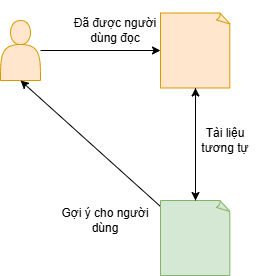
\includegraphics[width=\textwidth]{Images/CBF.png}
        \caption{Lọc dựa trên nội dung.}
        \label{fig:CBF}
    \end{subfigure}
    \hfill % Lệnh này tự động căn đều khoảng trống ở giữa 2 ảnh
    % Khung chứa ảnh 2 (chiếm 45% chiều rộng trang)
    \begin{subfigure}[b]{0.45\textwidth}
        \centering
        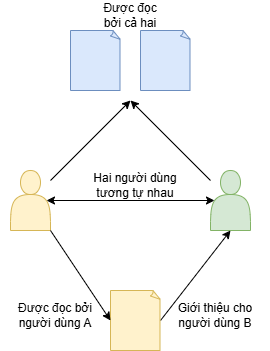
\includegraphics[width=\textwidth]{Images/CF.png}
        \caption{Lọc cộng tác.}
        \label{fig:CF}
    \end{subfigure}
    
    \vspace{0.3cm}
    \caption{Minh họa hai phương pháp gợi ý truyền thống.}
    \label{fig:traditional_methods}
\end{figure}

Phương pháp Lọc dựa trên nội dung, hay Content-Based Filtering, hoạt động dựa trên nguyên lý nhất quán về sở thích cá nhân. Kỹ thuật này trích xuất các đặc trưng nội tại của sản phẩm bao gồm văn bản, danh mục hoặc thương hiệu để xây dựng không gian vector, sau đó tính toán độ tương đồng với hồ sơ sở thích của người dùng \cite{18}. Ưu điểm chiến lược của phương pháp này là khả năng giải quyết triệt để bài toán Khởi động lạnh cho sản phẩm mới. Tuy nhiên, thuật toán sẽ bộc lộ hạn chế trong năng lực phân tích nội dung khi tiếp cận với các mặt hàng yêu cầu cảm nhận chủ quan tinh tế, ví dụ như việc đánh giá mức độ hài hước của hai cuốn truyện cười, hoặc khi xử lý những dữ liệu phi cấu trúc phức tạp như phim ảnh. Đồng thời thuật toán này có hiện tượng chuyên biệt hóa quá mức tạo ra vòng lặp gợi ý nhàm chán và có rào cản khởi động lạnh đối với người dùng mới.

Trái ngược với cách tiếp cận trên, phương pháp Lọc cộng tác, thường được biết đến với thuật ngữ Collaborative Filtering \cite{18}, bỏ qua hoàn toàn nội dung sản phẩm để tập trung khai thác các mẫu hành vi ẩn trong cộng đồng. Dựa trên ma trận tương tác giữa người dùng và mặt hàng, hệ thống áp dụng phương pháp láng giềng gần nhất thuộc nhóm tiếp cận dựa trên bộ nhớ, hoặc vận dụng các kỹ thuật nén không gian ẩn như Phân rã ma trận thuộc nhóm tiếp cận dựa trên mô hình để tìm ra sự đồng điệu về sở thích. Sức mạnh lớn nhất của kỹ thuật này là khả năng mang lại tính khám phá cao, giúp đề xuất những sản phẩm xuyên danh mục một cách chính xác. Mặc dù mang lại hiệu suất vượt trội, sự phụ thuộc tuyệt đối vào lịch sử tương tác khiến Lọc cộng tác hoàn toàn tê liệt trước bài toán Khởi động lạnh cho cả người dùng lẫn sản phẩm mới. Đồng thời, hệ thống sẽ gặp hiện tượng suy giảm hiệu năng nghiêm trọng khi ma trận dữ liệu trở nên quá thưa thớt ở quy mô công nghiệp.

\subsection{Hệ thống Gợi ý Lai}

Sự ra đời của hệ thống gợi ý lai đánh dấu bước phát triển quan trọng nhằm khắc phục các hạn chế cố hữu khi triển khai độc lập phương pháp lọc cộng tác hoặc lọc dựa trên nội dung. Mục tiêu cốt lõi của hướng tiếp cận này là tối ưu hóa hiệu suất dự đoán thông qua việc tổng hợp sức mạnh từ cả dữ liệu hành vi người dùng và các thông tin đặc tả phong phú của sản phẩm. Trong giai đoạn trước khi học sâu trở nên phổ biến, các kiến trúc lai truyền thống thường được áp dụng dựa trên ba chiến lược kết hợp chủ đạo nhằm dung hòa các thuật toán nền tảng.

Đầu tiên là phương pháp lai trọng số, được xem là kỹ thuật cộng gộp đơn giản nhất trong các mô hình lai. Cơ chế vận hành của nó dựa trên việc triển khai song song các mô hình thành phần, sau đó tính toán điểm số xếp hạng cuối cùng bằng tổng có trọng số của các kết quả dự đoán riêng lẻ\cite{18}. Mặc dù ưu điểm là dễ triển khai, phương pháp này gặp hạn chế lớn do giả định mối quan hệ giữa các mô hình luôn là tuyến tính và đòi hỏi quá trình tinh chỉnh tham số thủ công rất kỹ lưỡng để cân bằng hiệu quả giữa các thành phần.

Chiến lược thứ hai là phương pháp lai chuyển đổi, hoạt động tương tự như một cơ chế điều hướng thông minh dựa trên trạng thái dữ liệu thực tế. Hệ thống sẽ linh hoạt lựa chọn thuật toán phù hợp nhất cho từng ngữ cảnh cụ thể, điển hình là việc ưu tiên sử dụng lọc theo nội dung đối với người dùng mới để giải quyết vấn đề khởi động lạnh, sau đó tự động chuyển sang lọc cộng tác khi đã thu thập đủ lịch sử tương tác tin cậy\cite{18}. Tuy nhiên, nhược điểm của chiến lược này nằm ở sự thiếu tính liên tục, dẫn đến trải nghiệm gợi ý có thể bị đứt gãy hoặc thiếu sự mượt mà trong quá trình chuyển giao giữa các mô hình.

Chiến lược kết hợp đặc trưng đại diện cho một bước chuyển dịch quan trọng trong kiến trúc hệ thống gợi ý lai, nơi ranh giới giữa dữ liệu nội dung và dữ liệu hành vi được xóa bỏ để hướng tới một không gian biểu diễn thống nhất. Khác với các phương pháp lai ghép lỏng lẻo như lai trọng số hay lai chuyển đổi vốn xử lý các mô hình thành phần một cách độc lập, phương pháp này chủ động hợp nhất các nguồn thông tin ngay từ giai đoạn đầu vào. Mục tiêu cốt lõi là làm giàu không gian đặc trưng, cho phép thuật toán học được sự tương quan chéo giữa các đặc tính nội tại của sản phẩm với hành vi tương tác của người dùng, thay vì chỉ dựa vào các mã định danh thưa thớt.

Kế thừa và phát triển tư duy này để giải quyết triệt để bài toán khởi động lạnh, Kula\cite{20} đã giới thiệu mô hình LightFM, một kiến trúc lai hiệu quả kết hợp ưu điểm của cả lọc cộng tác và lọc theo nội dung. Điểm đột phá của LightFM nằm ở cơ chế biểu diễn vector linh hoạt, trong đó biểu diễn của một người dùng hoặc sản phẩm được xác định bằng tổng các vector nhúng của định danh và các vector nhúng của các thuộc tính mô tả đi kèm. Nhờ cơ chế cộng gộp này, hệ thống có khả năng suy luận độ tương đồng dựa trên các đặc điểm chung ngay cả khi sản phẩm đó chưa từng có lịch sử tương tác, đảm bảo luồng gợi ý được duy trì liên tục và chính xác cho các thực thể mới.

Tuy nhiên, mặc dù các phương pháp kết hợp đặc trưng như Factorization Machines hay LightFM đã đạt được những thành công nhất định, chúng vẫn tồn tại những hạn chế về khả năng biểu diễn các mẫu dữ liệu phức tạp. Như Cheng và cộng sự\cite{21} đã phân tích trong công trình về kiến trúc Wide \& Deep, các mô hình dựa trên tích vô hướng hoặc biến đổi tuyến tính thường thiên về khả năng ghi nhớ các mẫu đồng xuất hiện trong quá khứ nhưng lại hạn chế trong việc tổng quát hóa các mối quan hệ phi tuyến tính mức cao. Nhận định này đã mở đường cho sự phát triển của các kiến trúc mạng nơ-ron sâu hiện đại, nơi các lớp ẩn đa tầng được sử dụng để trích xuất và kết hợp đặc trưng một cách tinh vi hơn nhằm thấu hiểu sâu sắc ý định người dùng.

\subsection{Hệ thống gợi ý đa giai đoạn}

Trong bối cảnh các sàn thương mại điện tử hiện đại như Amazon, Alibaba hay Shopee đang lưu trữ hàng tỷ sản phẩm, việc xây dựng một hệ thống gợi ý vừa đảm bảo độ chính xác tuyệt đối, vừa đáp ứng được thời gian phản hồi theo thời gian thực là một thách thức cực kỳ lớn đối với các kỹ sư máy học. Nếu sử dụng một mô hình ngôn ngữ sâu sắc và phức tạp để tính toán độ tương quan cho toàn bộ kho dữ liệu mỗi khi người dùng thực hiện truy vấn, hệ thống sẽ gặp phải độ trễ không thể chấp nhận được, gây ảnh hưởng trực tiếp đến trải nghiệm và doanh thu. Để giải quyết mâu thuẫn giữa hiệu năng và độ chính xác, kiến trúc Gợi ý Đa giai đoạn đã ra đời và trở thành tiêu chuẩn công nghiệp phổ biến, giúp tối ưu hóa quá trình xử lý thông qua một cấu trúc hình phễu lọc giảm dần về số lượng nhưng tăng dần về độ tinh vi của thuật toán.

\begin{figure}[H]
\centering
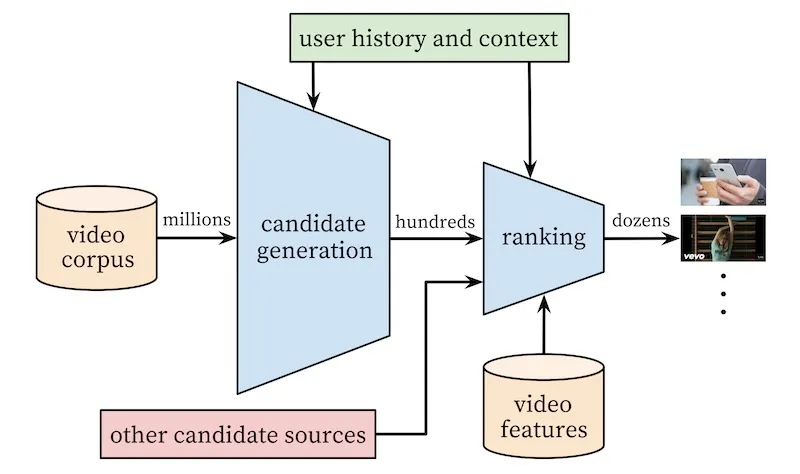
\includegraphics[width=0.85\textwidth]{Images/multi.png}
\vspace{1em}
\caption{Kiến trúc hình phễu tiêu biểu của hệ thống gợi ý đa giai đoạn}
\label{fig:multi_stage_funnel}
\end{figure}

Như hình \ref{fig:multi_stage_funnel}, hệ thống không cố gắng tìm ra kết quả tốt nhất ngay lập tức mà chia quy trình thành các pha tách biệt, trong đó nổi bật nhất là sự phối hợp giữa hai giai đoạn then chốt: Truy xuất (Retrieval) và Xếp hạng lại (Ranking/Reranking). Cách tiếp cận này lần đầu tiên được phổ biến rộng rãi thông qua công trình nghiên cứu kinh điển của Covington và các cộng sự tại Google (2016) về hệ thống gợi ý cho YouTube \cite{9}. Trong nghiên cứu này, các tác giả đã chỉ ra rằng việc sử dụng một mô hình đơn lẻ cho toàn bộ quy trình là không hiệu quả; thay vào đó, hệ thống cần một bộ lọc thô để loại bỏ hàng triệu thực thể không liên quan và những bộ lọc tinh phía sau để sắp xếp các ứng viên tiềm năng nhất vào vị trí hiển thị tối ưu.

Giai đoạn đầu tiên là Truy xuất đóng vai trò như một bộ lọc thô với nhiệm vụ sàng lọc nhanh chóng từ hàng triệu sản phẩm xuống còn khoảng vài trăm ứng viên. Tại giai đoạn này, tốc độ là yếu tố tiên quyết để đảm bảo tính thời gian thực. Kiến trúc chủ đạo thường được sử dụng là Bi-Encoder hay còn gọi là kiến trúc Two-Tower.

Trong kiến trúc này, tháp người dùng và tháp sản phẩm hoạt động độc lập, cho phép hệ thống tính toán trước và lưu trữ các embeddings của toàn bộ kho hàng vào cùng một không gian vector tiềm ẩn. Khi có truy vấn, hệ thống chỉ cần mã hóa câu lệnh người dùng và thực hiện các phép tính đại số đơn giản như tích vô hướng hoặc Cosine Similarity thông qua các thuật toán tìm kiếm ANN. Điểm mạnh của Bi-Encoder là khả năng quét qua hàng triệu thực thể chỉ trong vài mili-giây. Tuy nhiên, do áp dụng cơ chế Late Interaction, nơi truy vấn và sản phẩm không hề trao đổi thông tin với nhau trong quá trình mã hóa, mô hình thường bỏ lỡ các sắc thái ngữ nghĩa giao thoa chi tiết giữa hai đối tượng.

Ngay sau khi có được danh sách ứng viên từ pha Truy xuất, hệ thống chuyển sang giai đoạn Xếp hạng lại để thực hiện những tính toán chuyên sâu hơn trên tập dữ liệu đã được thu hẹp (thường từ vài chục đến vài trăm sản phẩm như mô tả trong sơ đồ hình phễu). Đây là giai đoạn mà độ chính xác được đặt lên hàng đầu nhằm đảm bảo những sản phẩm phù hợp nhất với ý định người dùng và cá nhân hóa sâu sắc sẽ được hiển thị ở những vị trí đầu tiên. Kiến trúc hiệu quả nhất cho giai đoạn này là Cross-Encoder. Khác với Bi-Encoder, Cross-Encoder nhận đầu vào là sự kết hợp đồng thời giữa câu truy vấn và thông tin sản phẩm, cho phép cơ chế Self-Attention của Transformer thực hiện Tương tác sớm. Từng token trong câu lệnh của người dùng có thể soi chiếu và tương tác trực tiếp với từng đặc trưng của sản phẩm ở mọi tầng của mạng nơ-ron. Cơ chế này giúp mô hình nắm bắt được những mối liên hệ ẩn ý, sự tương đồng ngữ nghĩa phức tạp và đặc biệt là khả năng cá nhân hóa dựa trên lịch sử hành vi mua sắm. Việc áp dụng Cross-Encoder ở giai đoạn Reranking giúp hệ thống đạt được sự tối ưu về mặt chất lượng, vì lúc này mô hình chỉ phải xử lý một lượng nhỏ ứng viên, cho phép sử dụng các kiến trúc nặng nề và phức tạp mà vẫn đảm bảo thời gian phản hồi tổng thể.

Sự kết hợp giữa Two-Tower và Cross-Encoder tạo nên một hệ chỉnh thể hoàn chỉnh, giúp hệ thống gợi ý vừa có thể quét qua quy mô dữ liệu khổng lồ, vừa có thể đưa ra những đề xuất mang tính cá nhân hóa cao độ. Kế thừa và tuân thủ trọn vẹn triết lý đa giai đoạn đó, đồ án này tiến hành triển khai kiến trúc Bi-Encoder làm nền tảng cho giai đoạn Truy xuất nhằm khoanh vùng tập ứng viên nhanh chóng, và áp dụng mô hình Cross-Encoder được tích hợp thêm các thành phần bổ trợ cho giai đoạn Xếp hạng lại. Việc ứng dụng cơ chế này ở pha cuối đóng vai trò như một mảnh ghép chiến lược, bởi nó không chỉ giữ được sức mạnh tương tác ngữ nghĩa sâu của Cross-Encoder truyền thống mà còn tích hợp được cơ chế Item Memory, từ đó tận dụng tối đa sức mạnh biểu diễn của mô hình ngôn ngữ trong việc cá nhân hóa sâu sắc nhu cầu của từng người dùng cuối.

\section{Các Hàm Mục tiêu}

Trong các hệ thống gợi ý hiện đại và tìm kiếm ngữ nghĩa, mục tiêu của học biểu diễn là học một hàm ánh xạ $f$ để đưa các thực thể (người dùng, sản phẩm) vào một không gian vector sao cho các thực thể có mối quan hệ tương quan sẽ nằm gần nhau về mặt hình học (độ tương đồng Cosine cao hoặc khoảng cách L2 thấp).

Để tối ưu hóa không gian này, việc lựa chọn hàm mục tiêu đóng vai trò then chốt. Nhóm đã nghiên cứu và triển khai ba nhóm hàm mục tiêu chính: Triplet Loss, InfoNCE (Contrastive Loss) và Cross-Entropy Loss.

\subsection{Triplet Loss}

Được phổ biến rộng rãi bởi Schroff và đồng nghiệp\cite{23} trong mô hình FaceNet cho bài toán nhận diện khuôn mặt, Triplet Loss là nền tảng của học sâu metric. Thay vì dự đoán xác suất, phương pháp này hướng tới việc tối ưu hóa khoảng cách hình học trong không gian vector. Mô hình nhận đầu vào là một bộ ba $(A, P, N)$ bao gồm: Anchor (Mẫu gốc), Positive (Mẫu cùng loại/người dùng thích) và Negative (Mẫu khác loại). Mục tiêu là đảm bảo khoảng cách giữa Anchor và Positive phải nhỏ hơn khoảng cách giữa Anchor và Negative một đoạn biên độ an toàn $\alpha$:
\begin{equation}
    \mathcal{L}_{\text{Triplet}} = \sum \max \left( 0, d(A, P)^2 - d(A, N)^2 + \alpha \right)
\end{equation}
Mặc dù giải quyết tốt vấn đề về thứ tự xếp hạng, Triplet Loss đối mặt với thách thức lớn về sự hội tụ. Hiệu suất của hàm này phụ thuộc cực đoan vào chiến lược lấy mẫu. Nếu chọn các mẫu âm quá dễ - tức là các sản phẩm hoàn toàn không liên quan, gradient sẽ nhanh chóng tiến về 0 và mô hình ngừng học. Ngược lại, việc tìm kiếm các mẫu âm khó Hard Negative Mining lại đòi hỏi chi phí tính toán rất lớn, làm chậm quá trình huấn luyện.

\subsection{InfoNCE}
InfoNCE (Information Noise-Contrastive Estimation) hay còn gọi là Contrastive loss, được chuẩn hóa trong kiến trúc SimCLR hay Two-Tower của Google\cite{8}. Thay vì chỉ so sánh một cặp $P - N$ duy nhất như Triplet Loss, InfoNCE coi bài toán là việc tìm đúng mẫu Positive trong một tập hợp gồm nhiều mẫu Negative.

Công thức toán học của InfoNCE:

\begin{equation}
    \mathcal{L}_{\text{InfoNCE}} = - \log \frac{\exp(\text{sim}(u, i^+) / \tau)}{\sum_{j=1}^{K} \exp(\text{sim}(u, i_j) / \tau)} \label{eq:infoNCE}
\end{equation}
Trong đó $\mathrm{sim}(.)$ là độ tương đồng Cosine, $\tau$ là tham số nhiệt độ để điều chỉnh độ nhạy của hàm phân phối xác suất.

\textbf{Ứng dụng trong đồ án:} Nhóm triển khai phiên bản \textbf{Symmetric Contrastive Loss}. Trong mỗi batch huấn luyện, các sản phẩm của những người dùng khác trong lô huấn luyện sẽ đóng vai trò là mẫu âm tính trong lô. Phương pháp này cho phép mô hình tận dụng tối đa dữ liệu ngay trong batch để tối ưu hóa, tăng tốc độ hội tụ và giúp không gian Embedding đạt được tính đồng nhất.

\subsection{Symmetric Explicit Contrastive Loss}

Dựa trên đặc thù của dữ liệu thương mại điện tử Amazon, việc chỉ sử dụng các mẫu âm tính ngẫu nhiên (những sản phẩm người dùng chưa từng biết tới) là chưa đủ để mô hình học được ranh giới sở thích tinh tế. Nhóm đề xuất sử dụng thêm \textbf{Explicit Negatives} được trích xuất trực tiếp từ lịch sử đánh giá của người dùng.

Trong đồ án này, tập dữ liệu tương tác được phân loại dựa trên mức độ hài lòng thực tế:
\begin{itemize}
    \item \textbf{Mẫu Positive:} Các sản phẩm đã tương tác và được người dùng đánh giá từ 3 sao trở lên ($\ge 3$). Đây là những sản phẩm thể hiện sự phù hợp với sở thích của người dùng.
    \item \textbf{Mẫu Explicit Negative:} Các sản phẩm người dùng đã mua nhưng đánh giá thấp (1 hoặc 2 sao). Khác với các mẫu âm tính ngẫu nhiên, đây là những tín hiệu từ chối mạnh, cho thấy người dùng thực sự không hài lòng với các thuộc tính của sản phẩm đó.
\end{itemize}

Trong hàm Loss này, bên cạnh các mẫu âm tính trong batch, nhóm đưa thêm các sản phẩm 1-2 sao này vào làm mẫu âm tính cứng. Công thức được mở rộng bằng cách nối kết điểm số của Explicit Negatives vào tập hợp logits trước khi đưa qua hàm Softmax:

\begin{equation}
    \text{logits}_{combined} = [\text{sim}(q, p), \text{sim}(q, n_1), \dots, \text{sim}(q, n_K), \text{sim}(q, n_{explicit})]
\end{equation}

Việc bổ sung này buộc mô hình phải học cách phân biệt sự khác biệt giữa sản phẩm người dùng yêu thích và sản phẩm họ ghét, thay vì chỉ phân biệt giữa thứ họ thích và thứ họ chưa biết". Kết quả là không gian vector được tinh chỉnh để đẩy người dùng ra xa khỏi những vùng không gian chứa các thuộc tính sản phẩm không phù hợp, nâng cao độ chính xác cho hệ thống gợi ý.

\subsection{Binary Cross Entropy}
Đây là hàm mất mát tiêu chuẩn được áp dụng rộng rãi trong các bài toán dự đoán tỷ lệ nhấp (CTR Prediction) và các mô hình Lọc cộng tác nơ-ron như đề xuất của Xiangnan He và cộng sự\cite{22}, nó cũng được sử dụng trong kiến trúc SASRec của Wang-Cheng Kang và Julian McAuley\cite{7}. Dưới góc độ tiếp cận theo điểm Pointwise Approach, hàm mục tiêu này chuyển đổi bài toán gợi ý thành bài toán phân loại nhị phân, trong đó mô hình xem xét mỗi cặp người dùng - sản phẩm $(u, i)$ như một biến cố độc lập. Mục tiêu là tối thiểu hóa sai số giữa nhãn thực tế $y_{ui}$ (nhận giá trị 1 nếu có tương tác, 0 nếu không) và xác suất dự đoán $p_{ui}$ của mô hình:
\begin{equation}
    \mathcal{L}_{\text{BCE}} = - \sum_{(u,i) \in \mathcal{D}} \left[ y_{ui} \cdot \log(p_{ui}) + (1 - y_{ui}) \cdot \log(1 - p_{ui}) \right]
\end{equation}
Trong đồ án, BCE Loss đóng vai trò là hàm mục tiêu cho giai đoạn Reranking. Sau khi Bi-Encoder thực hiện truy xuất thô để lọc ra Top-K sản phẩm tiềm năng với tốc độ cao, Cross-Encoder sẽ đánh giá lại các cặp (User, Item) này một cách kỹ lưỡng bằng BCE Loss để tinh chỉnh thứ hạng cuối cùng. Sự kết hợp này mang lại độ chính xác tối đa trước khi hệ thống trả kết quả gợi ý cho người dùng.

\section{Kiến trúc nền tảng: Transformer}

Năm 2017 đánh dấu một bước ngoặt lịch sử trong lĩnh vực trí tuệ nhân tạo khi kiến trúc Transformer chính thức được giới thiệu thông qua bài báo Attention Is All You Need \cite{12}. Khác biệt hoàn toàn so với các mạng nơ-ron tuần tự truyền thống vốn bị giới hạn bởi nút thắt cổ chai về tính toán và suy giảm khả năng ghi nhớ dài hạn, Transformer loại bỏ hoàn toàn các lớp truy hồi để phụ thuộc tuyệt đối vào cơ chế sự chú ý. Bước đột phá này cho phép mô hình xử lý dữ liệu song song trên quy mô khổng lồ, đồng thời thấu hiểu chính xác các mối quan hệ ngữ nghĩa xuyên suốt toàn bộ chuỗi đầu vào. Sự ra đời của kiến trúc ưu việt này không chỉ kiến tạo nền móng vững chắc cho các mô hình ngôn ngữ lớn hiện đại mà còn trực tiếp tái định hình phương pháp luận trong việc trích xuất đặc trưng đa phương thức đối với các hệ thống gợi ý tiên tiến.

\subsection{Cơ chế Scaled Dot-Product Self-Attention}
\label{subsec:scaled_attention}
Cơ chế vận hành cốt lõi tạo nên sức mạnh của các kiến trúc hiện đại là kỹ thuật Scaled Dot-Product Self-Attention. Về mặt toán học, với đầu vào là một chuỗi các vector nhúng $X \in \mathbb{R}^{n \times d}$, mô hình thực hiện phép chiếu không gian để biến $X$ thành ba ma trận thành phần bao gồm: Truy vấn $Q$, Khóa $K$ và Giá trị $V$. Quá trình tính toán trọng số sự chú ý được định nghĩa thông qua công thức:

\begin{equation}
    \text{Attention}(Q, K, V) = \text{softmax}\left(\frac{QK^T}{\sqrt{d_k}}\right)V
\end{equation}

Trong biểu thức này, tích vô hướng $QK^T$ đại diện cho mức độ tương đồng ngữ nghĩa, xác định mức độ mà mỗi phần tử cần chú ý đến các phần tử khác để cập nhật biểu diễn của chính nó. Đáng chú ý, phép chia cho căn bậc hai của chiều vector khóa $\sqrt{d_k}$ đóng vai trò là một kỹ thuật chuẩn hóa thiết yếu. Khi chiều dữ liệu $d_k$ lớn, giá trị tích vô hướng có xu hướng tăng trưởng mạnh về độ lớn, đẩy hàm Softmax vào vùng bão hòa nơi gradient tiệm cận 0, gây trở ngại cho quá trình tối ưu hóa. Việc chia tỷ lệ giúp ổn định phương sai của điểm số attention, đảm bảo mạng nơ-ron hội tụ hiệu quả hơn.

\subsection{Cơ chế Multi-Head Attention}
Tiếp nối cơ chế tự chú ý cốt lõi, Multi-Head Attention là một bước tiến kiến trúc quan trọng giúp mạng nơ-ron Transformer khắc phục giới hạn của việc chỉ có một góc nhìn duy nhất đối với dữ liệu đầu vào. Thay vì thực hiện một phép tính Softmax duy nhất trên các ma trận kích thước lớn, hệ thống sử dụng các ma trận trọng số riêng biệt để chiếu $Q$, $K$ và $V$ xuống các chiều dữ liệu nhỏ hơn, tạo thành $h$ đầu chú ý hoạt động song song. 

Công thức tổng quát của cơ chế này được biểu diễn như sau:
\begin{equation}
    \text{MultiHead}(Q, K, V) = \text{Concat}(\text{head}_1, \dots, \text{head}_h)W^O
\end{equation}

Trong đó, mỗi đầu chú ý $\text{head}_i$ được tính toán hoàn toàn độc lập thông qua phép nhân với các ma trận trọng số tương ứng $W_i^Q$, $W_i^K$, $W_i^V$:
\begin{equation}
    \text{head}_i = \text{Attention}(QW_i^Q, KW_i^K, VW_i^V)
\end{equation}

Sau khi tất cả các đầu hoàn thành quá trình tính toán, kết quả của chúng được ghép nối lại với nhau bằng toán tử $\text{Concat}$ để tạo thành một vector biểu diễn tổng hợp. Cuối cùng, vector này được nhân với một ma trận trọng số đầu ra $W^O$ nhằm khôi phục lại kích thước chiều ban đầu. Sự ưu việt của phương pháp này nằm ở chỗ nó cho phép mô hình thấu hiểu ngôn ngữ ở cấp độ đa chiều, trong đó mỗi đầu chú ý có thể tự do bắt sóng một khía cạnh ngữ nghĩa hoặc một quy luật đặc thù khác nhau của luồng dữ liệu.

\subsection{Cơ chế Mã hóa Vị trí}
\label{subsec:positional_encoding}
Một giới hạn đặc thù của các kiến trúc dựa trên sự chú ý thuần túy là tính bất biến với thứ tự. Phép toán tích vô hướng trong Self-Attention coi chuỗi đầu vào như một tập hợp các phần tử không có cấu trúc tuần tự, dẫn đến việc mô hình hoàn toàn mất đi nhận thức về vị trí tương đối hoặc tuyệt đối của dữ liệu. Nhược điểm này là một trở ngại chí mạng đối với các bài toán yêu cầu tính thứ tự nghiêm ngặt như xử lý ngôn ngữ tự nhiên hay dự đoán chuỗi hành vi người dùng.

Để khắc phục, kiến trúc Transformer tích hợp thêm một cơ chế Mã hóa Vị trí, tên tiếng Anh là Positional Encoding. Phương pháp này hoạt động bằng cách cộng trực tiếp một vector thông tin vị trí vào vector nhúng đặc trưng của từng phần tử đầu vào trước khi truyền vào mạng nơ-ron. Biểu diễn toán học của tín hiệu vị trí này thường được khởi tạo thông qua các hàm lượng giác chu kỳ:

\begin{equation}
    PE_{(pos, 2i)} = \sin\left(\frac{pos}{10000^{2i/d_{\text{model}}}}\right)
\end{equation}
\begin{equation}
    PE_{(pos, 2i+1)} = \cos\left(\frac{pos}{10000^{2i/d_{\text{model}}}}\right)
\end{equation}

Trong đó, $pos$ đại diện cho vị trí của phần tử trong chuỗi, $i$ là chỉ số chiều của vector và $d_{\text{model}}$ là tổng số chiều của không gian biểu diễn. Thông qua việc sử dụng các hàm sin và cosin với tần số biến thiên, cơ chế này ép mỗi tọa độ vị trí sinh ra một mẫu vector duy nhất. Khi được dung hợp vào dữ liệu gốc, nó cung cấp cho mô hình một hệ quy chiếu không gian và thời gian chuẩn xác, cho phép các đầu chú ý dễ dàng tính toán khoảng cách và nắm bắt quy luật tuần tự của chuỗi hành vi mà không làm thay đổi kiến trúc song song lõi của hệ thống.

\begin{figure}[H]
    \centering
    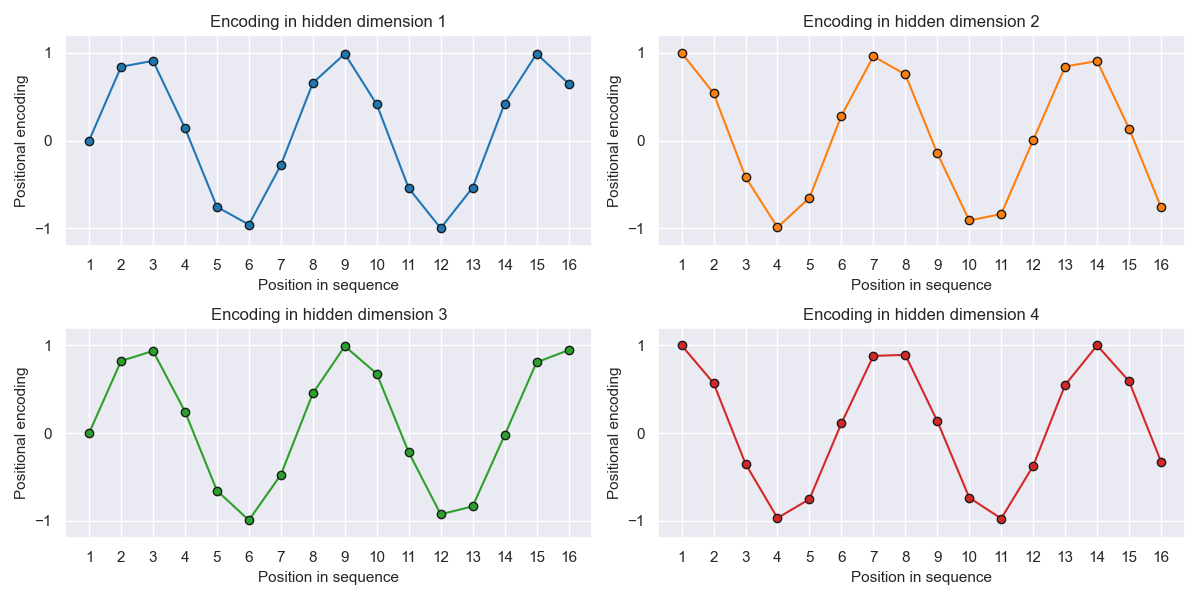
\includegraphics[width=1.0\textwidth]{Images/position_encoder.png}
    \vspace{0.3cm}
    \caption{Minh họa trực quan giá trị Positional Encoding trên 4 chiều ẩn đầu tiên. Các đường cong hình sin với tần số khác nhau giúp mô hình phân biệt vị trí trong chuỗi.}
    \label{fig:pos_encoding_vis}
\end{figure}

Hình \ref{fig:pos_encoding_vis} minh họa trực quan sự biến thiên giá trị của vector mã hóa vị trí trên bốn chiều ẩn đầu tiên đối với một chuỗi có độ dài $16$ bước. Các đồ thị cho thấy hàm lượng giác dao động trong khoảng từ $-1$ đến $1$ với tần số khác nhau tùy thuộc vào chỉ số của chiều không gian. Cụ thể, các chiều có chỉ số thấp thể hiện tần số dao động cao, trong khi các chiều cao hơn sở hữu bước sóng dài hơn. Cơ chế biến đổi tần số này kiến tạo nên một mẫu hình đặc trưng riêng biệt cho mỗi vị trí $pos$, hỗ trợ mô hình Transformer dễ dàng học được mối quan hệ vị trí tương đối giữa các token trong chuỗi.

\section{Biểu diễn Đa phương thức}
Trong kỷ nguyên dữ liệu lớn, thông tin về sản phẩm không còn bị giới hạn ở các mã định danh hay thuộc tính cấu trúc đơn giản, mà đã mở rộng sang các dạng dữ liệu phi cấu trúc phong phú như văn bản mô tả và hình ảnh minh họa. Học đa phương thức là phương pháp tiếp cận tiên tiến cho phép hệ thống tri nhận và thấu hiểu sâu sắc nội dung sản phẩm, từ đó xây dựng các vector biểu diễn embeddings giàu ngữ nghĩa. Cách tiếp cận này đặc biệt hiệu quả trong việc giải quyết bài toán cold-start đối với các sản phẩm mới chưa có lịch sử tương tác. Để khai thác hai luồng thông tin quan trọng nhất là ngôn ngữ và thị giác, đồ án áp dụng hai kiến trúc nền tảng đã chứng minh được hiệu quả vượt trội trong lĩnh vực này, lần lượt là BERT cho xử lý văn bản và ViT cho xử lý hình ảnh.

\subsection{Biểu diễn Văn bản: BERT}

Sự xuất hiện của mô hình BERT (Bidirectional Encoder Representations from Transformers)\cite{14} đã tạo ra một bước tiến quan trọng trong lĩnh vực xử lý ngôn ngữ tự nhiên, đặc biệt là ứng dụng trong việc trích xuất đặc trưng văn bản cho các hệ thống gợi ý hiện đại. Trước khi các mô hình ngôn ngữ lớn trở nên phổ biến, các phương pháp nhúng từ truyền thống như Word2Vec\cite{15} hay GloVe chủ yếu dựa trên cơ chế tạo ra các vector nhúng tĩnh. Hạn chế căn bản của cách tiếp cận này là việc gán một vector biểu diễn cố định duy nhất cho mỗi từ vựng, bất kể sự biến thiên về ngữ nghĩa trong các ngữ cảnh khác nhau.

Vấn đề này trở nên đặc biệt nghiêm trọng trong miền dữ liệu thương mại điện tử, nơi các từ khóa thường mang tính đa nghĩa cao. Điển hình như từ khóa "Chuột", ngữ nghĩa của nó thay đổi hoàn toàn khi xuất hiện trong cụm "Chuột máy tính Logitech" thuộc danh mục thiết bị điện tử so với cụm "Thuốc diệt chuột" thuộc danh mục hóa phẩm. Các mô hình tĩnh như Word2Vec không thể phân tách sự khác biệt này, dẫn đến sai lệch trong việc tính toán độ tương đồng sản phẩm. Ngược lại, BERT khắc phục triệt để nhược điểm trên thông qua cơ chế tạo ra các vector nhúng động, cho phép biểu diễn chính xác ngữ nghĩa của từ dựa trên sự phụ thuộc vào các từ lân cận trong câu.

Về mặt kiến trúc, BERT được xây dựng dựa trên sự chồng xếp của các lớp mã hóa trong kiến trúc Transformer. Khác biệt so với các mô hình tự hồi quy như GPT vốn chỉ xử lý thông tin đơn chiều từ trái sang phải, BERT áp dụng cơ chế Mô hình hóa ngôn ngữ che mặt nạ (Masked Language Modeling - MLM). Cơ chế này cho phép mô hình tiếp nhận và tổng hợp luồng thông tin ngữ cảnh hai chiều đồng thời, giúp nắm bắt cấu trúc cú pháp và ngữ nghĩa sâu sắc hơn. Như được minh họa chi tiết trong Hình \ref{fig:bert_architecture} \cite{14}, quy trình vận hành của BERT được chia thành hai giai đoạn kế tiếp nhau trên cùng một nền tảng kiến trúc thống nhất.
\begin{figure}[H]
    \centering
    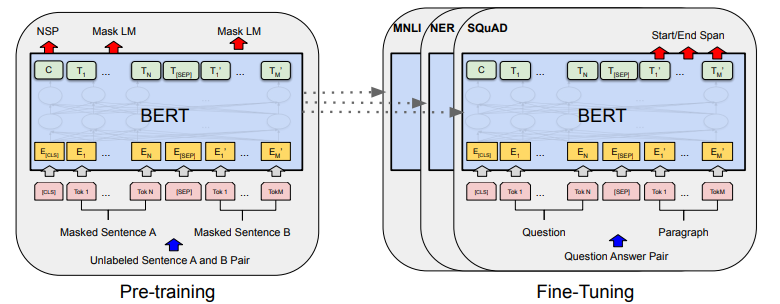
\includegraphics[width=0.9\textwidth]{Images/bert.png}
    \vspace{0.5cm}
    \caption{Quy trình Tiền huấn luyện và Tinh chỉnh của BERT.}
    \label{fig:bert_architecture}
\end{figure}

\noindent \textbf{Giai đoạn Tiền huấn luyện}

Giai đoạn tiền huấn luyện đóng vai trò nền tảng trong quy trình xây dựng mô hình, tại đó hệ thống tiếp thu các biểu diễn ngôn ngữ tổng quát thông qua việc khai thác khối lượng lớn dữ liệu văn bản thô chưa được gán nhãn. Quá trình học tập này vận hành dựa trên cơ chế tự giám sát, tập trung tối ưu hóa đồng thời hai tác vụ cốt lõi nhằm nắm bắt sâu sắc cấu trúc ngôn ngữ.

Đầu tiên là tác vụ Masked Language Modeling - MLM. Khác với phương pháp dự đoán từ tiếp theo theo tuần tự truyền thống, tác vụ này yêu cầu hệ thống phải khôi phục và tái tạo chính xác các đơn vị từ vựng đã bị che khuất ngẫu nhiên trong câu. Cơ chế này buộc mô hình phải tổng hợp và thấu hiểu ngữ cảnh hai chiều từ cả phía trước và phía sau của từ mục tiêu để đưa ra suy luận hợp lý nhất. Song song với đó là tác vụ dự đoán câu tiếp theo hay NSP, được thiết kế nhằm mục đích giúp mô hình thấu hiểu mối quan hệ logic và sự liên kết giữa các đoạn văn bản. Cụ thể, hệ thống học cách xác định xem một câu B bất kỳ có phải là câu nối tiếp thực tế về mặt ngữ nghĩa của câu A hay không, qua đó nắm bắt được cấu trúc diễn ngôn ở cấp độ cao hơn so với việc chỉ xử lý các từ ngữ riêng lẻ.

\noindent \textbf{Giai đoạn Tinh chỉnh}

Giai đoạn tinh chỉnh đóng vai trò là bước chuyển giao tri thức quan trọng, nơi mô hình áp dụng các biểu diễn ngôn ngữ tổng quát đã học được vào các tác vụ hạ nguồn cụ thể. Về mặt quy trình, thay vì khởi tạo ngẫu nhiên, mô hình kế thừa toàn bộ trọng số tham số từ giai đoạn tiền huấn luyện làm điểm bắt đầu, sau đó tiến hành tối ưu hóa tiếp tục trên các tập dữ liệu có gán nhãn chuyên biệt. Điểm mấu chốt là toàn bộ các tham số của mạng lưới đều được cập nhật đồng bộ trong quá trình này để thích nghi tốt nhất với đặc thù của từng bài toán riêng biệt. Trong phạm vi của hệ thống gợi ý, thay vì giải quyết các tác vụ ngôn ngữ tổng quát, quá trình tinh chỉnh được thiết kế chuyên biệt nhằm tối ưu hóa khả năng đọc hiểu tiêu đề và mô tả mặt hàng. Mục tiêu cuối cùng là trích xuất ra các vector đặc trưng văn bản chứa đựng trọn vẹn ngữ nghĩa sản phẩm, phục vụ trực tiếp cho việc xây dựng tháp sản phẩm.

Một đặc điểm kiến trúc nổi bật tạo nên sự thành công của BERT chính là tính nhất quán về cấu trúc. Hệ thống duy trì nguyên vẹn khối kiến trúc mã hóa Transformer đa tầng xuyên suốt quá trình huấn luyện sơ bộ và tinh chỉnh, đảm bảo luồng xử lý thông tin không bị gián đoạn. Sự thay đổi duy nhất chỉ diễn ra ở lớp đầu ra cuối cùng, nơi được thiết kế lại linh hoạt để tương thích với định dạng dự đoán của từng tác vụ đích, giúp mô hình đạt được hiệu suất cao mà không cần thay đổi đáng kể về mặt cấu trúc lõi.

Về cơ chế xử lý cốt lõi, thay vì sử dụng các mạng truy hồi truyền thống, BERT kế thừa trực tiếp sức mạnh từ kiến trúc Multi-Head Self-Attention đã được phân tích chi tiết tại Mục \ref{subsec:scaled_attention}. Điểm đột phá của mô hình nằm ở cách khai thác cơ chế sự chú ý này theo hướng hai chiều triệt để. Bằng việc tính toán trọng số thông qua các khối ma trận Truy vấn, Khóa và Giá trị, mỗi token trong câu đầu vào đều có khả năng quan sát và thu thập ngữ cảnh trực tiếp từ tất cả các token còn lại ở cả phía trước và phía sau nó cùng một lúc. 

Đồng thời, việc tận dụng kiến trúc chú ý đa đầu cho phép BERT tri giác thông tin văn bản từ nhiều không gian biểu diễn song song. Sự phân công nhiệm vụ tự động giữa các đầu chú ý, ví dụ một đầu chuyên bóc tách cấu trúc cú pháp trong khi đầu khác rà soát mối liên kết từ vựng tầm xa, giúp vector đầu ra của mô hình hội tụ đầy đủ các sắc thái ngôn ngữ. Nhờ sự kế thừa chặt chẽ này, BERT tạo ra các biểu diễn văn bản mang độ sâu ngữ nghĩa vượt trội, đáp ứng hoàn hảo yêu cầu khắt khe về việc thấu hiểu mô tả sản phẩm trong kiến trúc truy xuất đa phương thức.

Trong ngữ cảnh cụ thể của hệ thống gợi ý, mục tiêu đặt ra là thu được một vector đại diện duy nhất cho toàn bộ văn bản đầu vào. Để thực hiện điều này, BERT bổ sung một token đặc biệt ký hiệu là \texttt{[CLS]} vào vị trí đầu tiên của chuỗi. Sau khi đi qua toàn bộ các lớp mã hóa Transformer, vector đầu ra tương ứng với vị trí \texttt{[CLS]} này được coi là biểu diễn tổng hợp tinh túy nhất của cả câu:
\begin{equation}
    h_{\texttt{[CLS]}} = \text{BERT}(x_1, \dots, x_n)
\end{equation}
Vector $h_{\texttt{[CLS]}}$ này có khả năng nắm bắt được các đặc trưng ngữ nghĩa bậc cao như danh mục sản phẩm, tính năng nổi bật hay sắc thái cảm xúc trong bài đánh giá, mang lại hiệu quả vượt trội so với các phương pháp biểu diễn thô sơ như \textit{Bag-of-Words} truyền thống.

\subsection{Biểu diễn Hình ảnh: ViT}

Trong giai đoạn trước năm 2020, các kiến trúc mạng nơ-ron tích chập, viết tắt là CNN, với những đại diện tiêu biểu như ResNet hay EfficientNet được xem là chuẩn mực hàng đầu cho các tác vụ thị giác máy tính. Thành công này chủ yếu bắt nguồn từ khả năng khai thác hiệu quả các thiên kiến quy nạp về tính cục bộ và tính bất biến tịnh tiến đặc trưng của dữ liệu hình ảnh. Đối lập với bức tranh đó, kiến trúc Transformer\cite{12} lại đang khẳng định vị thế độc tôn và tạo ra những bước tiến vượt bậc trong lĩnh vực xử lý ngôn ngữ tự nhiên.

Bối cảnh công nghệ này đã thúc đẩy sự ra đời của Vision Transformer, hay còn gọi là ViT, nhằm giải quyết câu hỏi khoa học về tính khả thi của việc áp dụng trực tiếp kiến trúc Transformer thuần túy lên dữ liệu thị giác. Cách tiếp cận của ViT mang tính đột phá khi loại bỏ hoàn toàn sự phụ thuộc vào các lớp tích chập truyền thống để chuyển sang mô hình hóa bức ảnh dưới dạng một chuỗi các phần tử tuần tự, tương tự như cơ chế xử lý các đoạn văn bản.

Quyết định thay thế mạng tích chập truyền thống bằng kiến trúc Vision Transformer được củng cố bởi nghiên cứu mang tính đột phá của Dosovitskiy và cộng sự\cite{11}. Trong công trình này, nhóm tác giả đã chứng minh tính khả thi và hiệu quả vượt trội của việc áp dụng cơ chế tự chú ý trực tiếp lên dữ liệu hình ảnh quy mô lớn. Thay vì phụ thuộc vào các thiên kiến quy nạp về tính cục bộ như trong mạng ResNet hay EfficientNet, phương pháp này xử lý bức ảnh như một chuỗi các mảnh ghép độc lập, cho phép mô hình nắm bắt được các mối quan hệ ngữ nghĩa toàn cục giữa các vùng ảnh xa nhau ngay từ những lớp đầu tiên.

Rào cản kỹ thuật lớn nhất khi chuyển giao kiến trúc Transformer từ miền dữ liệu chuỗi sang dữ liệu hình ảnh nằm ở gánh nặng tính toán khổng lồ. Do cơ chế tự chú ý sở hữu độ phức tạp thuật toán bậc hai $\mathcal{O}(N^2)$ tỷ lệ thuận với số lượng phần tử đầu vào $N$, việc mô hình hóa trực tiếp từng điểm ảnh đơn lẻ như một đơn vị \textit{token} sẽ dẫn đến sự bùng nổ về chi phí tài nguyên. Đơn cử, một hình ảnh có kích thước tiêu chuẩn $224 \times 224$ sẽ tạo ra một chuỗi đầu vào lên tới 50.176 phần tử, khiến việc xây dựng ma trận chú ý trở nên bất khả thi đối với năng lực phần cứng hiện tại.

Mô hình Vision Transformer giải quyết triệt để vấn đề này thông qua kỹ thuật phân mảnh hay còn gọi là \textit{Patching}. Quy trình xử lý bắt đầu bằng việc chia nhỏ hình ảnh đầu vào $I \in \mathbb{R}^{H \times W \times C}$ thành một lưới các vùng cục bộ không chồng lấn có kích thước cố định $P \times P$, tạo ra tổng cộng $N = \frac{HW}{P^2}$ mảnh con. Tiếp theo, mỗi mảnh ảnh này được trải phẳng thành một vector một chiều và được đưa qua một phép chiếu tuyến tính có thể học được để ánh xạ vào không gian biểu diễn tiềm ẩn với số chiều $D$. Cuối cùng, nhằm mục đích khôi phục và bảo toàn thông tin về cấu trúc không gian vốn bị phá vỡ trong quá trình trải phẳng, các vector mã hóa vị trí $E_{\text{pos}}$ được cộng bổ sung trực tiếp vào các vector đặc trưng của từng mảnh trước khi đưa vào khối mã hóa Transformer. Quy trình xử lý chi tiết được mô tả trực quan thông qua Hình \ref{fig:vit_architecture} \cite{11}.

\begin{figure}[H]
    \centering
    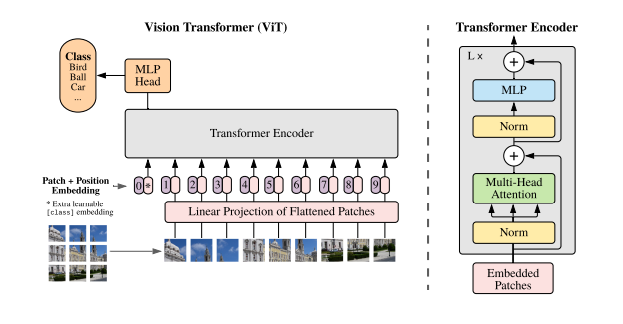
\includegraphics[width=0.9\textwidth]{Images/Vit.png}
    \vspace{0.5cm}
    \caption{Sơ đồ kiến trúc Vision Transformer.}
    \label{fig:vit_architecture}
\end{figure}

Bước tiếp theo là việc khởi tạo token phân loại. Một vector tham số có thể học được, thường được ký hiệu là token lớp, được chèn vào vị trí đầu tiên của chuỗi các vector mảnh ảnh. Token đặc biệt này đóng vai trò như một bộ thu nhận thông tin toàn cục; sau khi đi qua toàn bộ mạng nơ-ron, trạng thái đầu ra tại vị trí này sẽ được sử dụng làm đại diện tổng quát duy nhất cho toàn bộ bức ảnh, tương tự như cơ chế của token CLS trong mô hình ngôn ngữ BERT.

Chuỗi vector kết hợp này sau đó được đưa vào khối mã hóa Transformer Encoder, bao gồm nhiều lớp xử lý lặp lại liên tiếp. Trong mỗi lớp, cơ chế chú ý đa đầu đóng vai trò hạt nhân, cho phép mỗi mảnh ảnh có khả năng quan sát và liên kết ngữ nghĩa với tất cả các mảnh ảnh khác, bất kể khoảng cách không gian giữa chúng. Dữ liệu sau đó tiếp tục đi qua mạng nơ-ron truyền thẳng MLP để trích xuất các đặc trưng bậc cao. Để đảm bảo sự ổn định và khả năng hội tụ của quá trình huấn luyện sâu, kỹ thuật chuẩn hóa lớp Layer Normalization được áp dụng trước mỗi khối chức năng, kết hợp cùng các kết nối tắt nhằm duy trì dòng chảy thông tin và hạn chế hiện tượng triệt tiêu đạo hàm.

Cuối cùng, tại lớp đầu ra của khối mã hóa, chỉ duy nhất vector ứng với vị trí của token phân loại được trích xuất. Vector này mang trong mình thông tin ngữ nghĩa cô đọng nhất của bức ảnh và được đưa vào khối MLP Head để thực hiện các tác vụ đích như phân loại đối tượng hoặc tạo vector biểu diễn cho hệ thống gợi ý.\\

Sự khác biệt nền tảng định hình nên ưu thế của Vision Transformer so với mạng tích chập CNN nằm ở bản chất của trường tiếp nhận thông tin. Đối với các mạng tích chập truyền thống, trường tiếp nhận mang tính chất cục bộ nghiêm ngặt, nghĩa là các lớp tích chập khởi đầu chỉ có khả năng ghi nhận và xử lý tín hiệu từ các điểm ảnh lân cận. Sự tổng hợp thông tin toàn cục chỉ có thể đạt được một cách gián tiếp và thụ động thông qua quá trình chồng xếp nhiều lớp mạng sâu nhằm mở rộng dần vùng quan sát. Ngược lại, Vision Transformer tận dụng sức mạnh của cơ chế tự chú ý để phá vỡ giới hạn không gian này. Ngay từ lớp xử lý đầu tiên, mỗi mảnh ảnh đã thiết lập được sự tương tác trực tiếp với tất cả các mảnh ảnh khác, cho phép mô hình có cái nhìn toàn cảnh tức thời về đối tượng.

Đặc tính kỹ thuật này mang lại ý nghĩa quan trọng trong ngữ cảnh của bài toán gợi ý sản phẩm, đặc biệt đối với các ngành hàng đề cao tính thẩm mỹ như thời trang hay nội thất. Trong những lĩnh vực này, vẻ đẹp và giá trị của sản phẩm thường không chỉ nằm ở các chi tiết riêng lẻ mà phụ thuộc vào bố cục tổng thể cùng sự phối hợp giữa các thành phần nằm cách xa nhau, chẳng hạn như sự tương thích giữa cổ áo và gấu váy hay sự đồng điệu giữa màu sắc giày và họa tiết thương hiệu. Năng lực thấu hiểu các mối quan hệ ngữ nghĩa toàn cục và phức tạp này cho phép Vision Transformer trích xuất được các vector đặc trưng giàu thông tin hơn, mang lại hiệu quả vượt trội cho tác vụ gợi ý so với các phương pháp tích chập truyền thống.

\subsection{Cơ chế Hợp nhất Không gian Vector}
\label{sec:attention_theory}

Một sản phẩm trên thực tế có thể có nhiều hình thức biểu diễn như văn bản, hình ảnh, video. Nghiên cứu của Radford \cite{16} đã khẳng định tầm quan trọng của việc khai thác đa phương thức để hiểu sâu ngữ nghĩa đối tượng. Tuy nhiên, thay vì chỉ so khớp đơn thuần, việc hợp nhất các đặc trưng này thành một biểu diễn duy nhất là yêu cầu bắt buộc đối với tháp sản phẩm trong kiến trúc Two-Tower. Hình \ref{fig:fusion_architecture} \cite{16} mô tả kiến trúc hợp nhất được đề xuất.
\begin{figure}[H]
    \centering
    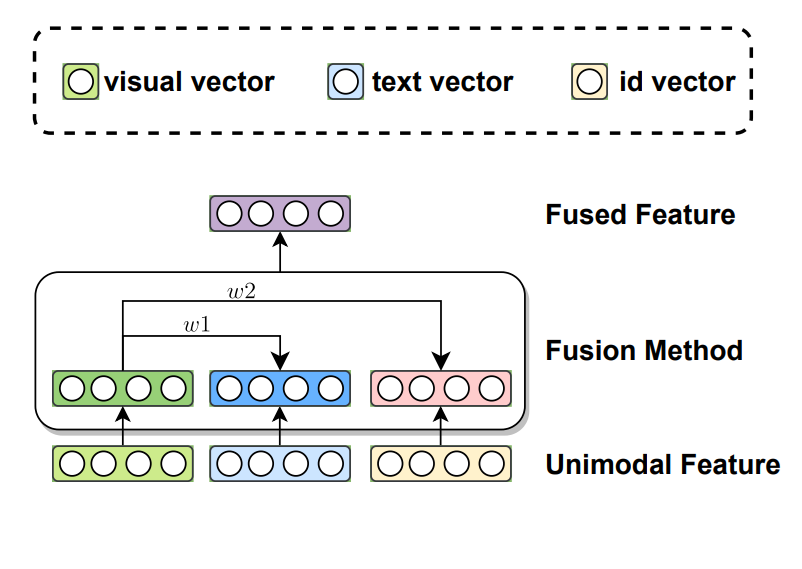
\includegraphics[width=0.9\textwidth]{Images/fusion.png}
    \vspace{0.5cm}
    \caption{Sơ đồ kiến trúc Multi-Modality Fusion.}
    \label{fig:fusion_architecture}
\end{figure}

Hạn chế căn bản của các phương pháp hợp nhất truyền thống như phép nối vector hay phép cộng trung bình nằm ở giả định cứng nhắc rằng mức độ quan trọng của hình ảnh và văn bản là tương đương nhau đối với mọi sản phẩm. Trong thực tế dữ liệu thương mại điện tử luôn tồn tại sự bất cân xứng về chất lượng thông tin khi một số mặt hàng sở hữu hình ảnh trực quan sắc nét nhưng phần mô tả lại sơ sài hoặc ngược lại. Để giải quyết vấn đề này đồ án áp dụng cơ chế Hợp nhất có cổng hay còn gọi là Gated Fusion được phát triển dựa trên nền tảng lý thuyết mạng nơ-ron đa phương thức của Arevalo và cộng sự\cite{24}.

Quy trình xử lý dữ liệu để tạo ra vector đại diện sản phẩm được thực hiện qua ba giai đoạn tuần tự, đảm bảo tính đồng bộ về mặt toán học giữa các luồng dữ liệu khác biệt.

Đầu tiên là giai đoạn đồng bộ hóa không gian biểu diễn. Xuất phát từ thực tế rằng đầu ra từ các bộ mã hóa hình ảnh và văn bản (như ViT cho ảnh và BERT cho văn bản) thường sở hữu số chiều khác nhau và nằm trong các phân phối đặc trưng riêng biệt, hệ thống cần áp dụng phép chiếu tuyến tính để dung hòa sự khác biệt này. Cụ thể, hai ma trận trọng số $\mathbf{W}_v$ và $\mathbf{W}_t$ được sử dụng để ánh xạ các đặc trưng thô về cùng một không gian vector tiềm ẩn có kích thước cố định $d$, tạo tiền đề cho sự tương tác trực tiếp:
\begin{align}
    \mathbf{v}_I &= \tanh(\mathbf{W}_v \cdot I_{\text{raw}} + \mathbf{b}_v) \\
    \mathbf{v}_T &= \tanh(\mathbf{W}_t \cdot T_{\text{raw}} + \mathbf{b}_t)
\end{align}
Tiếp theo, các vector đặc trưng sau khi đồng bộ được đưa vào cơ chế Hợp nhất có cổng (\textit{Gated Mechanism}). Đây là thành phần cốt lõi của mô hình, đóng vai trò như một van điều tiết thông minh nhằm xác định mức độ quan trọng của từng luồng thông tin. Một giá trị cổng kiểm soát $z$ được tính toán dựa trên sự kết hợp của cả hai loại dữ liệu, sử dụng hàm kích hoạt Sigmoid $\sigma$ để nén giá trị về khoảng $(0, 1)$:
\begin{equation}
    z = \sigma(\mathbf{W}_z \cdot [\mathbf{v}_I, \mathbf{v}_T] + \mathbf{b}_z)
\end{equation}
Dựa trên giá trị cổng này, vector hợp nhất $\mathbf{v}_{\text{fusion}}$ được xác định bằng tổ hợp tuyến tính có trọng số. Cơ chế này cho phép mô hình linh hoạt chuyển đổi sự tập trung; khi $z$ tiệm cận $1$, hệ thống sẽ ưu tiên khai thác tín hiệu thị giác và ngược lại sẽ dựa nhiều vào văn bản khi $z$ tiến về $0$:
\begin{equation}
    \mathbf{v}_{\text{fusion}} = z \odot \mathbf{v}_I + (1 - z) \odot \mathbf{v}_T
\end{equation}

Cuối cùng, để hoàn thiện biểu diễn của sản phẩm, vector hợp nhất $\mathbf{v}_{\text{fusion}}$ trải qua bước chuẩn hóa theo chuẩn $L_2$ nhằm tạo ra vector đầu ra $\mathbf{v}_{\text{item}}$:
\begin{equation}
    \mathbf{v}_{\text{item}} = \frac{\mathbf{v}_{\text{fusion}}}{\|\mathbf{v}_{\text{fusion}}\|_2}
\end{equation}
Bước xử lý này đảm bảo độ dài của mọi vector đại diện đều bằng $1$. Về mặt hình học, điều này giúp phép nhân vô hướng với vector người dùng ở giai đoạn truy xuất sau này trở thành thước đo độ tương đồng Cosine chuẩn xác, đồng thời góp phần ổn định đáng kể quá trình huấn luyện của mạng nơ-ron.

\section{Nắm bắt chuỗi hành vi trong ResSys}

\subsection{Sự tiến hóa của các Hệ thống Gợi ý Tuần tự: Từ Markov đến RNN}

Trong bối cảnh thương mại điện tử, sở thích của người dùng là một quá trình động, thay đổi liên tục theo thời gian và chịu ảnh hưởng mạnh mẽ bởi ngữ cảnh ngắn hạn. Trước khi kỷ nguyên học sâu bùng nổ, Chuỗi Markov đóng vai trò là nền tảng lý thuyết chủ đạo. Mô hình này, tiêu biểu như FPMC \cite{26}, xem lịch sử người dùng là các trạng thái chuyển đổi và đưa ra giả định theo tính chất Markov bậc một: hành động tiếp theo chỉ phụ thuộc duy nhất vào hành động ngay trước đó. Dù hiệu quả trong việc nắm bắt tương tác ngắn hạn giữa các cặp sản phẩm liền kề, Chuỗi Markov lại tỏ ra yếu kém trong việc ghi nhớ các chuỗi hành vi dài.

Để giải quyết bài toán phụ thuộc xa, Mạng nơ-ron tái phát RNN và các biến thể như GRU, LSTM đã được áp dụng. Điển hình là kiến trúc GRU4Rec \cite{30}, cho phép mô hình hóa toàn bộ lịch sử hành vi thành một chuỗi liên tục thông qua cơ chế cập nhật trạng thái ẩn, qua đó trích xuất được sở thích dài hạn của người dùng. Mặc dù vượt trội hơn Markov, kiến trúc RNN vẫn tồn tại những nhược điểm chí mạng: bản chất tính toán tuần tự khiến quá trình huấn luyện không thể song song hóa trên các phần cứng hiện đại như GPU, đồng thời hiện tượng triệt tiêu đạo hàm vẫn xảy ra với các chuỗi quá dài. Những rào cản phần cứng và thuật toán này chính là động lực thúc đẩy sự chuyển dịch công nghệ sang các kiến trúc dựa trên cơ chế Tự chú ý trong giai đoạn sau này.

\subsection{Kiến trúc SASRec}

Dựa trên sự thành công vang dội của cơ chế Attention trong xử lý ngôn ngữ tự nhiên, Kang và McAuley (2018) \cite{7} đã đề xuất mô hình SASRec. Đây là kiến trúc được đồ án lựa chọn làm nòng cốt cho Tháp Người dùng. SASRec thay thế hoàn toàn các lớp hồi quy bằng cơ chế Tự chú ý (Self-Attention), cho phép mô hình xác định trọng số quan trọng của từng sản phẩm trong quá khứ đối với sản phẩm mục tiêu dựa trên mối quan hệ ngữ nghĩa thay vì khoảng cách vị trí cố định. Nội dung trong mục này nói về mô hình SASRec của Kang và McAuley \cite{7}.

Mô hình SASRec vận hành thông qua một chuỗi các tầng xử lý tuần tự, khởi đầu với Tầng Nhúng. Kế thừa trực tiếp nguyên lý đã được phân tích tại Mục \ref{subsec:positional_encoding} về giới hạn nhận thức thứ tự của mạng Transformer, hệ thống bắt buộc phải tích hợp thông tin vị trí vào chuỗi đầu vào. Cụ thể, mô hình thực hiện phép cộng trực tiếp ma trận biểu diễn đặc trưng của sản phẩm $M$ với một ma trận vị trí có thể học được $P$, tạo thành một không gian biểu diễn tổng hợp $\hat{E} = M + P$.

Ngay sau bước chuẩn bị dữ liệu, ma trận tổng hợp này được truyền thẳng vào khối mạng Self-Attention. Dựa trên nền tảng toán học của cơ chế sự chú ý đã được định nghĩa chi tiết tại Mục \ref{subsec:scaled_attention}, SASRec tiến hành điều chỉnh kỹ thuật để tương thích tuyệt đối với bài toán chuỗi thời gian. Cụ thể, mô hình tích hợp thêm cơ chế che chắn nhân quả nhằm giới hạn tầm nhìn của mạng nơ-ron. Cơ chế này ép buộc các đầu chú ý chỉ được phép quét và tính toán mức độ tương quan đối với các sản phẩm mà người dùng đã tương tác trong quá khứ, triệt tiêu hoàn toàn hiện tượng rò rỉ thông tin từ tương lai. Nhờ sự kết hợp này, SASRec có khả năng nắm bắt chính xác dòng chảy biến thiên trong sở thích mua sắm của khách hàng ở từng thời điểm cụ thể. Một yếu tố kỹ thuật then chốt tại đây là việc áp dụng Mặt nạ nhân quả (\textit{Causal Masking}). Cơ chế này đảm bảo rằng khi dự đoán tại thời điểm $t$, mô hình chỉ được phép tiếp cận thông tin từ thời điểm $1$ đến $t$, ngăn chặn tuyệt đối việc rò rỉ thông tin từ tương lai và bảo toàn tính nhân quả của dữ liệu chuỗi.

Để khai thác các đặc trưng sâu hơn sau lớp Attention, mô hình tích hợp Mạng truyền thẳng từng điểm (\textit{Point-wise Feed-Forward Network}). Mạng này thực hiện các phép biến đổi phi tuyến cho từng vị trí một cách độc lập nhưng chia sẻ chung bộ trọng số, giúp mô hình nắm bắt các tương tác phức tạp giữa các chiều ẩn. Kiến trúc tổng thể của SASRec được hình thành bằng cách xếp chồng $b$ khối xử lý như vậy nhằm giải quyết vấn đề quá khớp và mất ổn định khi huấn luyện mạng sâu, nhóm tác giả áp dụng cấu trúc tương tự Transformer bao gồm Chuẩn hóa lớp (\textit{Layer Normalization}) để ổn định phân phối, Dropout để điều hòa quá trình học, và Kết nối tắt (\textit{Residual Connections}) để hỗ trợ lan truyền thông tin. Toàn bộ quy trình này được mô hình hóa qua công thức tổng quát cho mỗi lớp con $g$:
\begin{equation}
    g(x) = x + \text{Dropout}(g(\text{LayerNorm}(x)))
\end{equation}
như được mô tả trong tài liệu của Kang và McAuley.

Tại Tầng Dự đoán cuối cùng, sau khi đi qua $b$ khối xử lý, vector đại diện $\mathbf{F}_t^{(b)}$ tại bước $t$ sẽ được sử dụng để dự đoán sản phẩm tiếp theo. Điểm số tương quan $r_{i,t}$ được xác định bằng tích vô hướng giữa vector đại diện này và vector nhúng của sản phẩm mục tiêu $\mathbf{N}_i$. Để tối ưu hóa kích thước mô hình và hạn chế quá khớp, SASRec áp dụng chiến lược Shared Item Embedding, tức là sử dụng chung một ma trận nhúng cho cả đầu vào và đầu ra ($\mathbf{N}=\mathbf{M}$). Các tác giả lập luận rằng tính phi tuyến mạnh mẽ của mạng truyền thẳng là đủ để mô hình giải quyết vấn đề bất đối xứng (mua điện thoại thì có thể đề xuất ốp lưng nhưng mua ốp lưng thì không đề xuất điện thoại) trong các chuyển đổi hành vi mua sắm mà không cần thiết phải tách biệt hai ma trận này.

Dựa trên các kết quả thực nghiệm được công bố bởi Kang và McAuley, mô hình SASRec đã chứng minh được hiệu năng vượt trội so với các kiến trúc tiền nhiệm như GRU4Rec hay Caser nhờ vào hai ưu thế kỹ thuật then chốt.

Đầu tiên là khả năng nắm bắt các phụ thuộc dài hạn trong chuỗi hành vi. Đối với các mạng hồi quy truyền thống, thông tin buộc phải lan truyền tuần tự qua từng bước thời gian, tạo ra độ dài đường dẫn tỷ lệ thuận với độ dài chuỗi $\mathcal{O}(n)$. Ngược lại, cơ chế Tự chú ý cho phép thiết lập kết nối trực tiếp giữa hai sản phẩm bất kỳ bất kể khoảng cách vị trí. Đặc tính này rút ngắn độ dài đường truyền tín hiệu xuống mức hằng số $\mathcal{O}(1)$, giúp mô hình duy trì và truy xuất hiệu quả các sở thích người dùng đã hình thành từ quá khứ xa mà không bị suy hao thông tin.

Ưu điểm thứ hai nằm ở hiệu suất tính toán và khả năng mở rộng. Khác với tính chất tuần tự bắt buộc của mạng hồi quy khiến quá trình xử lý không thể tận dụng triệt để sức mạnh của GPU, các phép toán ma trận trong SASRec có thể được thực thi song song trên toàn bộ chiều dài chuỗi. Sự cải tiến này mang lại lợi ích to lớn về mặt tốc độ; các thử nghiệm cho thấy thời gian huấn luyện của SASRec nhanh hơn gấp mười lần so với các mô hình dựa trên mạng hồi quy hoặc tích chập, cho phép hệ thống dễ dàng mở rộng để xử lý các tập dữ liệu quy mô lớn.

\subsection{Kiến trúc Two tower cho Truy xuất Ứng viên}

\noindent \textbf{Bối cảnh và Vấn đề Quy mô}

Trong các hệ sinh thái thương mại điện tử quy mô lớn, thách thức kỹ thuật trọng yếu luôn nằm ở giai đoạn truy xuất (Retrieval). Tại đây, hệ thống buộc phải sàng lọc ra hàng trăm ứng viên tiềm năng từ một không gian dữ liệu khổng lồ chứa hàng triệu mặt hàng, với yêu cầu khắt khe về độ trễ tối thiểu, thường phải dưới 100 mili giây.

Trước bài toán này, các phương pháp truyền thống như Phân rã ma trận đã bộc lộ giới hạn do không thể nắm bắt các tương tác phi tuyến tính phức tạp. Quan trọng hơn, ngay cả các mô hình học sâu hiện đại như kiến trúc SASRec nguyên bản \cite{7} cũng vấp phải rào cản lớn khi triển khai thực tế. Do thiết kế theo hướng dự đoán đầu cuối (end-to-end classification) với chiến lược Shared Item Embedding, SASRec gốc trói buộc quá trình nội suy chuỗi hành vi của người dùng với ma trận định danh của toàn bộ sản phẩm vào cùng một đồ thị tính toán. Cấu trúc đóng gói này dẫn đến hai hệ lụy: thứ nhất, nó cản trở việc tích hợp các đặc trưng đa phương thức (văn bản, hình ảnh) để giải quyết bài toán cold-start; thứ hai, nó khiến việc quét và chấm điểm toàn bộ danh mục hàng triệu sản phẩm trong thời gian thực trở thành một gánh nặng tính toán bất khả thi.

Để giải quyết bài toán này, kiến trúc Mạng nơ-ron Hai tháp, hay còn được biết đến với tên gọi Bi-Encoder, đã trở thành chuẩn mực công nghiệp hiện đại. Mô hình này được tiên phong ứng dụng bởi YouTube \cite{9} và sau đó được tối ưu hóa hoàn thiện bởi Google \cite{8} cho các tác vụ xếp hạng quy mô lớn.

\vspace{0.3cm}

\noindent \textbf{Cấu trúc Mạng nơ-ron Hai tháp}

Về mặt bản chất, kiến trúc Hai tháp hoạt động dựa trên nguyên lý tách biệt quá trình mã hóa thành hai luồng xử lý độc lập nhằm tối ưu hóa tốc độ truy vấn. Cụ thể, hệ thống bao gồm Tháp Người dùng được ký hiệu là bộ mã hóa $f_\theta$, chịu trách nhiệm tổng hợp hồ sơ cá nhân và lịch sử hành vi để tạo ra vector biểu diễn người dùng $\mathbf{u}$ thuộc không gian $\mathbb{R}^d$. Song song với đó, Tháp Sản phẩm với bộ mã hóa $g_\phi$ tập trung khai thác các đặc trưng nội tại của vật phẩm để xây dựng vector biểu diễn tương ứng $\mathbf{v}$.

Điểm đặc trưng cốt lõi phân biệt thiết kế này với các mô hình khác là cơ chế tương tác muộn. Hai mạng nơ-ron hoàn toàn không chia sẻ thông tin hay tham số trong suốt quá trình trích xuất đặc trưng, mà chỉ thực hiện so khớp ở lớp cuối cùng. Tại đây, độ tương đồng hay mức độ phù hợp giữa người dùng và sản phẩm được ước lượng thông qua phép tính tích vô hướng đơn giản \cite{7}:
\begin{equation}
    s(x,y) = \langle u(x, \theta), v(y, \theta) \rangle
\end{equation}
Trong đó, $u(x, \theta)$ là hàm ánh xạ đặc trưng người dùng $x$, và $v(y, \theta)$ là hàm ánh xạ đặc trưng sản phẩm $y$ dựa trên bộ tham số mô hình $\theta$.

Cơ chế này cho phép hệ thống tính toán trước và lập chỉ mục các vector sản phẩm, giúp giảm đáng kể chi phí tính toán trực tuyến trong giai đoạn truy xuất thời gian thực.

\vspace{0.3cm}

\noindent \textbf{Chiến lược Huấn luyện: Học Tương phản}

Trong các kiến trúc Two-Tower hiện đại, chiến lược huấn luyện đã có sự chuyển dịch từ bài toán phân loại nhị phân truyền thống sang khuôn khổ Học tương phản (Contrastive Learning). Thách thức lớn nhất đối với các hệ thống truy xuất quy mô lớn nằm ở hàm mục tiêu: việc tính toán hàm Softmax trên toàn bộ không gian ứng viên (có thể lên tới hàng triệu sản phẩm) để xác định mẫu âm là bất khả thi về mặt tài nguyên tính toán và độ trễ. Để giải quyết vấn đề này, đồ án áp dụng giải pháp được đề xuất bởi Yi và cộng sự (2019) \cite{8}, sử dụng hàm mất mát Sampled Softmax kết hợp với kỹ thuật lấy mẫu âm trong lô.

Kỹ thuật này hoạt động dựa trên giả định thống kê rằng trong một lô dữ liệu ngẫu nhiên, các cặp người dùng và sản phẩm không tương ứng có xác suất rất cao là không liên quan đến nhau. Thay vì tiêu tốn chi phí để truy xuất và đào (mine) các mẫu âm từ kho dữ liệu bên ngoài, hệ thống tận dụng chính các sản phẩm của người dùng khác trong cùng một lô để làm mẫu âm.

Cụ thể, xét một lô dữ liệu có kích thước $B$. Với mỗi cặp mẫu dương $(\mathbf{u}_i, \mathbf{v}_i)$ (tương ứng với người dùng $i$ và sản phẩm thực tế $i$):
\begin{itemize}
    \item \textbf{Mẫu dương:} Là chính vector sản phẩm $\mathbf{v}_i$. Mục tiêu của mô hình là tối đa hóa độ tương đồng $s(\mathbf{u}_i, \mathbf{v}_i)$.
    \item \textbf{Mẫu âm:} Là tập hợp toàn bộ các vector sản phẩm $\mathbf{v}_j$ (với $j \neq i$) thuộc về các mẫu dữ liệu khác trong cùng batch đó. Như vậy, mỗi người dùng sẽ được so sánh với $1$ mẫu dương và $(B-1)$ mẫu âm nhân tạo này.
\end{itemize}

Để tối ưu hóa quá trình học biểu diễn vector, hệ thống sử dụng hàm mất mát InfoNCE (\ref{eq:infoNCE}). Hàm này có nhiệm vụ tối đa hóa xác suất dự đoán đúng sản phẩm mục tiêu $\mathbf{v}_i$ trong khi giảm thiểu xác suất của tập hợp $B-1$ sản phẩm nhiễu.

Phương pháp này không chỉ giải quyết triệt để bài toán hiệu năng tính toán mà còn được chứng minh là giúp mô hình học được các không gian biểu diễn phân tách tốt hơn, nhờ vào sự đa dạng và ngẫu nhiên của các mẫu âm được cập nhật liên tục trong mỗi bước huấn luyện.

\vspace{0.3cm}

\noindent \textbf{Ưu điểm về Triển khai Thực tế}

Lý do kiến trúc Two-Tower trở thành chuẩn mực thống trị trong bài toán Truy xuất bắt nguồn từ khả năng tách biệt hoàn toàn quá trình tính toán giữa hai thực thể người dùng và sản phẩm. Đặc tính kỹ thuật này cho phép tối ưu hóa quy trình xử lý thông qua hai giai đoạn riêng biệt. Trong giai đoạn ngoại tuyến (offline), nhờ sự độc lập của Tháp Sản phẩm, hệ thống có thể thực hiện tính toán trước vector biểu diễn cho toàn bộ không gian hàng hóa—có thể lên tới hàng triệu phần tử—và lưu trữ chúng dưới dạng chỉ mục tối ưu trong các cơ sở dữ liệu vector chuyên dụng như Milvus hay Faiss.

Chiến lược này tạo tiền đề cho hiệu suất vượt trội trong giai đoạn phục vụ trực tuyến (online serving). Khi nhận yêu cầu, hệ thống chỉ cần thực thi suy luận một lần duy nhất tại Tháp Người dùng để tạo ra vector truy vấn. Sau đó, thay vì phải quét toàn bộ cơ sở dữ liệu, việc xác định Top-K ứng viên tiềm năng được thực hiện thông qua các thuật toán ANN. Cơ chế này cho phép hệ thống duy trì độ trễ phản hồi ở mức dưới mili-giây, đồng thời đảm bảo tốc độ truy xuất không bị suy giảm tuyến tính khi quy mô kho hàng tăng lên, giải quyết triệt để bài toán về khả năng mở rộng của các hệ thống gợi ý hiện đại \cite{9}.

\section{Mô hình xếp hạng lại Reranking}
Sau khi giai đoạn Retrieval hoàn thành nhiệm vụ thu hẹp không gian tìm kiếm từ hàng triệu sản phẩm xuống một tập hợp ứng viên giới hạn, hệ thống đòi hỏi một cơ chế tinh vi hơn để phân tích chính xác mức độ phù hợp của từng ứng viên đối với nhu cầu của người dùng. Giai đoạn Reranking đảm nhận vai trò định chuẩn này. Việc chỉ sắp xếp lại vài chục đến vài trăm kết quả cho phép hệ thống triển khai các mô hình ngôn ngữ có độ phức tạp tính toán cao, mà điển hình và mạnh mẽ nhất hiện nay là kiến trúc Cross-Encoder.

\subsection{Lý thuyết Cross Encoder}

Mô hình Cross-Encoder là một kiến trúc mạng nơ-ron học sâu được xây dựng trực tiếp trên nền tảng của khối mã hóa (Encoder) thuộc mô hình Transformer, do Vaswani và cộng sự đề xuất vào năm 2017 \cite{49}. Sự trỗi dậy mạnh mẽ của Cross-Encoder trong lĩnh vực xếp hạng thông tin bắt đầu từ khi Nogueira và Cho (2019) ứng dụng thành công kiến trúc BERT vào bài toán đánh giá mức độ liên quan của văn bản \cite{50}. Nguyên lý hoạt động cốt lõi của Cross-Encoder nằm ở cách nó xử lý dữ liệu đầu vào và khai thác cơ chế tự chú ý.

\begin{figure}[H]
    \centering
    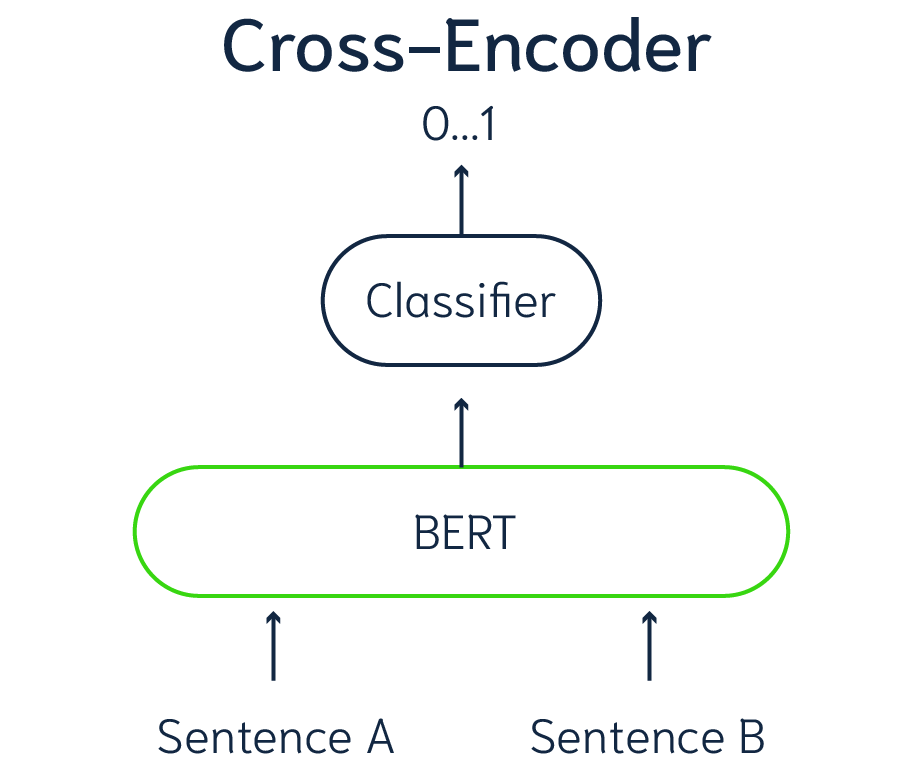
\includegraphics[width=0.5\textwidth]{Images/cross-encoder.png}
    \vspace{1em}
    \caption{Kiến trúc tổng quan của mô hình Cross-Encoder}
    \label{fig:cross_encoder_arch}
    
\end{figure}

Thay vì mã hóa độc lập từng đối tượng, Cross-Encoder yêu cầu ghép nối trực tiếp câu truy vấn ($Query$) và thông tin sản phẩm ($Item$) thành một chuỗi duy nhất trước khi đưa vào mô hình. Chuỗi đầu vào này thường được định dạng bằng các token đặc biệt, ví dụ như [CLS] Query [SEP] Item [SEP]. Ngay từ những lớp đầu tiên của mạng Transformer, cơ chế Tương tác sớm đã được kích hoạt. Thông qua ma trận Self-Attention, mỗi một từ khóa trong câu truy vấn đều có khả năng quan sát, tính toán trọng số và tương tác trực tiếp với toàn bộ các từ khóa nằm trong phần mô tả sản phẩm, và ngược lại. Quá trình này được lặp đi lặp lại qua nhiều tầng nơ-ron, giúp hệ thống không chỉ đối khớp từ khóa một cách máy móc mà còn thấu hiểu được ngữ cảnh, cấu trúc cú pháp và các hàm ý liên kết phức tạp.

Kết quả của toàn bộ quá trình tương tác chéo này được hội tụ vào token đặc biệt [CLS] ở tầng biểu diễn cuối cùng. Vector biểu diễn của token này mang theo toàn bộ thông tin tổng hợp về mối quan hệ ngữ nghĩa giữa $Query$ và $Item$. Cuối cùng, vector này được đưa qua một mạng nơ-ron truyền thẳng (Feed-Forward Network) kết hợp với hàm kích hoạt để chiếu thành một giá trị vô hướng duy nhất. Giá trị này đại diện cho điểm số xếp hạng, phản ánh chính xác mức độ liên quan của sản phẩm đối với mục tiêu tìm kiếm của người dùng.

\subsection{So sánh Cross Encoder và Bi Encoder}

Để hiểu rõ lý do tại sao kiến trúc hệ thống hiện đại bắt buộc phải duy trì hai giai đoạn với hai mô hình khác biệt, cần phải phân tích sự tương phản sâu sắc về cơ chế hoạt động cũng như sự đánh đổi giữa Cross-Encoder và Bi-Encoder. Nghiên cứu của Reimers và Gurevych (2019) về Sentence-BERT đã chỉ ra một cách hệ thống những ranh giới kỹ thuật này \cite{51}.

\begin{figure}[H]
    \centering
    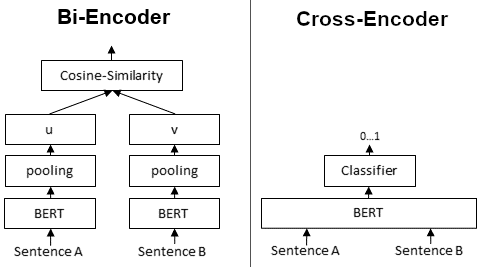
\includegraphics[width=1\textwidth]{Images/Bi_vs_Cross-Encoder.png}
    \vspace{1em}
    \caption{So sánh sự khác biệt giữa kiến trúc Bi-Encoder và Cross-Encoder}
    \label{fig:bi_vs_cross_comparison}
\end{figure}

Bi-Encoder, kiến trúc chủ đạo của giai đoạn Truy xuất, hoạt động dựa trên cơ chế Tương tác muộn. Nó sử dụng hai mạng Transformer độc lập để mã hóa câu truy vấn và sản phẩm thành hai vector dày đặc riêng biệt trong cùng một không gian học thuật. Sự so sánh chỉ diễn ra ở bước cuối cùng thông qua các phép tính đơn giản như độ tương đồng Cosine. Lợi thế tuyệt đối của Bi-Encoder là khả năng tính toán trước. Mọi sản phẩm trong kho đều được chuyển thành vector và lập chỉ mục từ trước, do đó khi có truy vấn, hệ thống chỉ mất vài mili giây để tìm ra các láng giềng gần nhất. Tuy nhiên, cái giá phải trả cho tốc độ là sự suy giảm về khả năng biểu diễn ngữ nghĩa. Việc nén toàn bộ ý nghĩa của một văn bản dài vào một vector có kích thước cố định gây ra hiện tượng thắt cổ chai thông tin. Mô hình mất đi khả năng đối khớp chính xác ở cấp độ từ vựng, dễ dẫn đến sai lệch khi người dùng tìm kiếm các sản phẩm có sự khác biệt rất nhỏ về từ ngữ nhưng khác biệt lớn về bản chất.

Ngược lại, Cross-Encoder khắc phục hoàn toàn nhược điểm này bằng cơ chế Tương tác sớm. Bằng cách cho phép các luồng thông tin giao thoa ngay từ đầu, nó duy trì được bức tranh toàn cảnh về mặt từ vựng và ngữ pháp. Ví dụ, trong ngữ cảnh thương mại điện tử, truy vấn "ốp lưng iPhone 15" và sản phẩm "iPhone 15 màu đen tặng kèm ốp lưng" có thể bị Bi-Encoder đánh giá là rất giống nhau vì không gian vector chứa nhiều từ khóa tương đồng. Tuy nhiên, Cross-Encoder với sự chú ý sâu sắc sẽ nhận ra vai trò chủ thể của cụm "ốp lưng" trong truy vấn không khớp với vai trò phụ trợ của nó trong tên sản phẩm, từ đó cho điểm xếp hạng thấp hơn.

Mặc dù có độ chính xác vượt trội, Cross-Encoder lại gặp phải rào cản chí mạng về khối lượng tính toán. Vì câu truy vấn và sản phẩm phải được ghép nối để tính toán lại từ đầu, độ phức tạp của cơ chế Self-Attention tăng lên theo bình phương độ dài chuỗi đầu vào. Việc áp dụng Cross-Encoder để so sánh một truy vấn với hàng triệu sản phẩm sẽ tiêu tốn một lượng tài nguyên và thời gian khổng lồ, vượt ra ngoài khả năng đáp ứng thời gian thực.

Chính sự bù trừ này đã định hình nên kiến trúc gợi ý đa giai đoạn. Bi-Encoder đóng vai trò như hệ thống lọc nhanh nhẹn, chấp nhận độ sai số nhất định để mang về một tập ứng viên khả thi từ biển dữ liệu rộng lớn. Trong khi đó, Cross-Encoder có vai trò Reranking. Bằng cách chỉ tập trung sức mạnh xử lý vào một số lượng ít các sản phẩm tiềm năng nhất, Cross-Encoder tối đa hóa được độ chính xác của kết quả đầu ra, đảm bảo những sản phẩm hiển thị ở các vị trí top đầu là những lựa chọn hoàn hảo nhất, nâng cao đáng kể tỷ lệ chuyển đổi và trải nghiệm mua sắm của người dùng.

\section{Ứng dụng Mô hình Ngôn ngữ Lớn trong Hệ thống Gợi ý}

Trong những năm gần đây, sự bùng nổ của các Mô hình Ngôn ngữ Lớn đã mở ra một hướng đi hoàn toàn mới cho lĩnh vực Hệ thống Gợi ý. Khác với các mô hình học máy truyền thống thường chỉ tập trung vào việc khai phá ma trận tương tác User-Item hoặc các đặc trưng rời rạc, LLM mang đến khả năng xử lý và suy luận trực tiếp trên ngôn ngữ tự nhiên, biến bài toán gợi ý khô khan thành một cuộc hội thoại tương tác mượt mà.

\subsection{Tổng quan về khả năng hiểu ngữ cảnh của LLM}

Sức mạnh cốt lõi của LLM nằm ở khả năng đọc hiểu và nắm bắt ngữ cảnh phức tạp thông qua hàng tỷ tham số được huấn luyện trên lượng dữ liệu khổng lồ. Trong ngữ cảnh của hệ thống gợi ý, LLM thể hiện những ưu điểm vượt trội sau:

\begin{itemize}
    \item \textbf{Xử lý dữ liệu văn bản phong phú:} Các mô hình gợi ý truyền thống gặp khó khăn trong việc hiểu sâu các nội dung văn bản dài như bài đánh giá, mô tả sản phẩm chi tiết hay lịch sử chat của người dùng. Ngược lại, LLM có thể dễ dàng trích xuất các thông tin ẩn như cảm xúc, sở thích cá nhân, và thậm chí là ý định mua sắm từ những đoạn văn bản này.
    \item \textbf{Suy luận ngữ nghĩa sâu:} LLM không chỉ khớp từ khóa mà còn hiểu được sự tương đồng về mặt ý nghĩa. Ví dụ, nếu người dùng tìm kiếm "đồ giữ ấm đi phượt mùa đông", LLM hiểu rằng người dùng đang cần áo khoác gió, mũ len, hoặc găng tay cách nhiệt, dù trong lịch sử của họ chưa từng xuất hiện cụm từ này.
    \item \textbf{Giải quyết vấn đề Zero-shot/Few-shot:} Nhờ kiến thức nền tảng rộng lớn, LLM có khả năng đưa ra gợi ý khá chính xác ngay cả với những sản phẩm mới hoặc người dùng mới chỉ dựa trên một vài thông tin mô tả cơ bản hoặc thậm chí không cần dữ liệu lịch sử tương tác.
\end{itemize}

\subsection{Kỹ thuật Prompting trong Hệ thống Gợi ý}

Để khai thác tối đa sức mạnh của LLM, \textbf{Prompt Engineering} là một yếu tố không thể thiếu. Việc thiết kế prompt giống như cách ta lập trình LLM bằng ngôn ngữ tự nhiên. Trong hệ thống gợi ý, các kỹ thuật prompting phổ biến bao gồm:

\begin{itemize}
    \item \textbf{In-context Learning:} Cung cấp cho LLM một vài ví dụ về lịch sử tương tác của người dùng ngay trong câu lệnh. Ví dụ: \textit{"Người dùng A đã mua [Điện thoại X, Ốp lưng Y]. Gợi ý sản phẩm tiếp theo cho A..."}. Cách này giúp LLM nắm bắt mẫu hành vi mà không cần cập nhật lại trọng số mô hình.
    \item \textbf{Chain-of-Thought:} Khuyến khích LLM giải thích từng bước logic trước khi đưa ra kết quả cuối cùng. Bằng cách thêm cụm từ \textit{"Hãy suy nghĩ từng bước một"}, LLM sẽ phân tích: vì sao người dùng thích sản phẩm này, đặc điểm nào phù hợp, từ đó giúp kết quả gợi ý chính xác và có tính thuyết phục cao hơn.
    \item \textbf{Role-playing:} Gán cho LLM một định danh cụ thể, ví dụ: \textit{"Bạn là một chuyên gia tư vấn thời trang AI..."}. Kỹ thuật này giúp định hình tông giọng và khoanh vùng không gian ngữ nghĩa, giúp kết quả trả về chuyên nghiệp và sát với lĩnh vực của hệ thống.
\end{itemize}

\subsection{Định hướng ứng dụng LLM trong Đồ án}

Nhận thấy tiềm năng to lớn của LLM, nhóm đồ án đã quyết định tích hợp công nghệ này vào hệ thống để giải quyết hai bài toán then chốt, nhằm nâng cao tính tương tác và độ chính xác của quy trình Reranking.

\textbf{Thứ nhất: Tự động sinh truy vấn huấn luyện cho Cross-Encoder} \\
Để huấn luyện mô hình Cross-Encoder phục vụ cho việc Reranking, hệ thống cần một lượng lớn dữ liệu dạng cặp \texttt{(Câu truy vấn - Tài liệu)}. Tuy nhiên, trong tập dữ liệu e-commerce (như Amazon), chúng ta thường chỉ có thông tin sản phẩm và lịch sử mua hàng, thiếu hẳn câu truy vấn thực tế của người dùng. Nhóm sử dụng LLM để đọc mô tả sản phẩm và tự động "tưởng tượng" ra các câu hỏi/truy vấn đa dạng mà người dùng có thể gõ để tìm kiếm sản phẩm đó. Việc tạo ra tập dữ liệu tổng hợp (Synthetic Data) này giúp Cross-Encoder học được sự liên kết ngữ nghĩa phong phú giữa nhu cầu tự nhiên và mô tả kỹ thuật.

\textbf{Thứ hai: Giải thích kết quả gợi ý} \\
Một trong những điểm yếu của các mô hình Deep Learning là tính "hộp đen", người dùng không biết vì sao họ lại được gợi ý sản phẩm này. Nhóm ứng dụng LLM ở bước cuối cùng của pipeline: sau khi hệ thống (qua Bi-Encoder và Cross-Encoder) đã chọn ra top các sản phẩm phù hợp nhất, LLM sẽ nhận đầu vào là lịch sử người dùng và thông tin các sản phẩm top đầu. Từ đó, LLM tổng hợp và sinh ra một đoạn văn bản ngắn, cá nhân hóa, giải thích lý do cụ thể vì sao sản phẩm này lại hoàn hảo dành cho họ (ví dụ: \textit{"Dựa trên việc bạn vừa mua một chiếc lều cắm trại, chúng tôi gợi ý chiếc đèn pin này vì nó có khả năng chống nước và thời lượng pin phù hợp cho những chuyến đi qua đêm"}). Điều này giúp tăng cường độ tin cậy và sự hài lòng của người dùng đối với hệ thống.
\newpage
\chapter{Phương pháp đề xuất}
\section{Kiến trúc tổng thể}

Hệ thống được thiết kế linh hoạt để tiếp nhận đầu vào đa dạng, cho phép người dùng tìm kiếm thông qua các câu truy vấn văn bản hoặc tải lên hình ảnh trực tiếp. Dựa trên những dữ liệu đầu vào này, hệ thống sẽ phân tích và đề xuất các sản phẩm chất lượng cao, đảm bảo sự tương thích sát sao nhất với nhu cầu và sở thích cá nhân của từng người dùng. Để hiện thực hóa điều này, nhóm sử dụng bộ dữ liệu Amazon Reviews làm nền tảng huấn luyện. Đây là một tập dữ liệu phong phú bao gồm các đặc trưng từ phía người dùng như nội dung đánh giá, điểm xếp hạng, và mức độ hữu ích của đánh giá đó, kết hợp cùng siêu dữ liệu sản phẩm item metadata như mô tả chi tiết, giá bán và hình ảnh gốc; tất cả được liên kết chặt chẽ với nhau thông qua mã định danh sản phẩm.

Về mặt phương pháp hoạt động, đồ án xây dựng một quy trình xử lý hiện đại kết hợp giữa kiến trúc Two-Tower và LLM nhằm đạt được độ chính xác cao trong việc gợi ý dựa trên hành vi mua sắm quá khứ. Phương pháp Two-Tower (hay Bi-Encoder) là một kiến trúc mạng nơ-ron tiên tiến được sử dụng rộng rãi trong các hệ thống gợi ý và tìm kiếm thông tin quy mô lớn, đóng vai trò then chốt trong giai đoạn truy xuất ứng viên. Kiến trúc này vận hành dựa trên hai nhánh mạng nơ-ron độc lập hoạt động song song: Tháp người dùng (User Tower) chịu trách nhiệm mã hóa các đặc trưng về hành vi, lịch sử và ngữ cảnh của người dùng, trong khi Tháp sản phẩm (Item Tower) xử lý các thông tin thuộc tính đa phương thức của sản phẩm như hình ảnh, văn bản mô tả hay thông số kỹ thuật. Cả hai tháp đều có nhiệm vụ chuyển đổi dữ liệu đầu vào phức tạp thành các vector embedding nén trong cùng một không gian tiềm ẩn, và mức độ phù hợp giữa người dùng và sản phẩm được xác định ở bước cuối cùng thông qua phép tính tích vô hướng hoặc độ tương đồng cosine. Ưu điểm vượt trội của Two-Tower nằm ở khả năng tách biệt quá trình tính toán, cho phép hệ thống lập chỉ mục trước hàng triệu vector sản phẩm, từ đó giải quyết bài toán tìm kiếm và gợi ý trong thời gian thực với độ trễ cực thấp mà vẫn đảm bảo nắm bắt được các mối quan hệ ngữ nghĩa sâu sắc.

\begin{figure}[H]
    \centering
    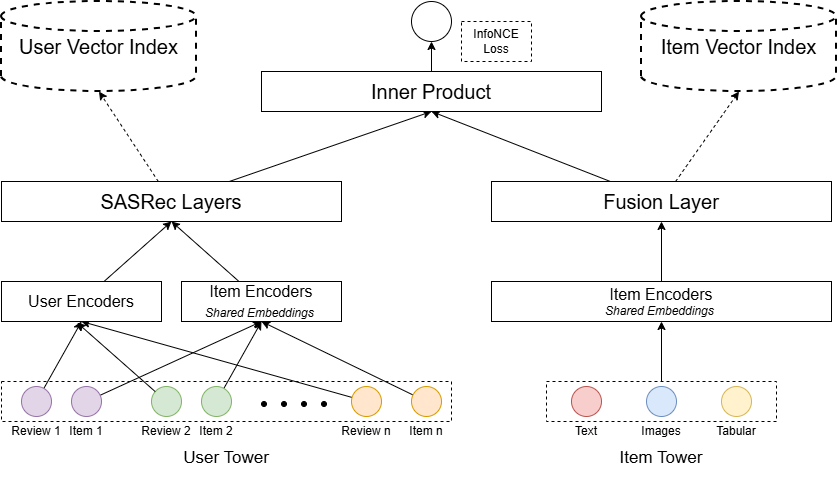
\includegraphics[width=0.8\textwidth]{Images/two_tower_model.png}
    \caption{Mô hình two-tower}
    \label{fig:overall_arch}
\end{figure}

Hình \ref{fig:overall_arch} minh họa kiến trúc tổng quát của mô hình đề xuất, được xây dựng dựa trên khung làm việc  Mạng nơ-ron Hai tháp. Mục tiêu cốt lõi của thiết kế này là tách biệt quá trình mã hóa Người dùng (User Modeling) và Sản phẩm (Item Modeling) thành hai luồng xử lý độc lập, cho phép tối ưu hóa hiệu năng trong giai đoạn truy xuất thời gian thực.

Luồng xử lý của hệ thống được chia thành hai nhánh chính:

\noindent \textbf{1. Tháp Người dùng (User Tower - Nhánh bên trái):}
Tháp này chịu trách nhiệm mô hình hóa sở thích người dùng dựa trên chuỗi lịch sử hành vi. Điểm cải tiến trong kiến trúc này là đầu vào không chỉ bao gồm định danh sản phẩm (Item ID) đơn thuần, mà là một chuỗi các cặp dữ liệu \textbf{(Review + Item)}.
\begin{itemize}
    \item Mỗi tương tác quá khứ được biểu diễn kết hợp giữa đặc trưng sản phẩm và nội dung đánh giá (Review) tương ứng, giúp mô hình nắm bắt được ngữ nghĩa và thái độ của người dùng tại thời điểm đó.
    \item Các thông tin này đi qua các bộ mã hóa User Encoders (nơi chứa khối xử lý chuỗi SASRec) và được tổng hợp tại lớp \textit{Fusion Layer} để tạo ra vector đại diện người dùng cuối cùng $\mathbf{u}$.
\end{itemize}

\noindent \textbf{2. Tháp Sản phẩm (Item Tower - Nhánh bên phải):}
Tháp này chịu trách nhiệm mã hóa các đặc trưng đa phương thức của một sản phẩm ứng viên (Candidate Item).
\begin{itemize}
    \item Đầu vào bao gồm dữ liệu văn bản (Text), hình ảnh (Images) và dữ liệu bảng (Tabular).
    \item Để đảm bảo tính nhất quán của không gian vector, hệ thống áp dụng kỹ thuật \textbf{Shared Embeddings} (Chia sẻ trọng số nhúng) cho các Item ID giữa hai tháp.
    \item Tương tự, các đặc trưng này được tổng hợp để tạo ra vector đại diện sản phẩm $\mathbf{v}$.
\end{itemize}

\noindent \textbf{3. Cơ chế Tương tác và Huấn luyện:} Hai tháp hoạt động song song và hoàn toàn không chia sẻ thông tin trong quá trình tính toán (Late Interaction). Tại lớp cuối cùng, sự tương đồng giữa người dùng và sản phẩm được tính toán thông qua tích vô hướng (Inner Product).

Mô hình được huấn luyện bằng hàm mất mát InfoNCE Loss theo nguyên lý Học tương phản. Sau khi huấn luyện, các vector người dùng và sản phẩm sẽ được lập chỉ mục vào các Cơ sở dữ liệu Vector (Vector Index) để phục vụ cho bài toán tìm kiếm láng giềng gần nhất (ANN Search).

Trên cơ sở các biểu diễn vector đặc trưng đã được trích xuất và đồng bộ hóa từ hai nhánh của mô hình, hệ thống chuyển sang giai đoạn truy xuất ứng viên thông qua cơ chế tính toán độ tương đồng trong không gian vector. Hình \ref{fig:retrieval} mô tả quá trình này.

\begin{figure}[H]
    \centering
    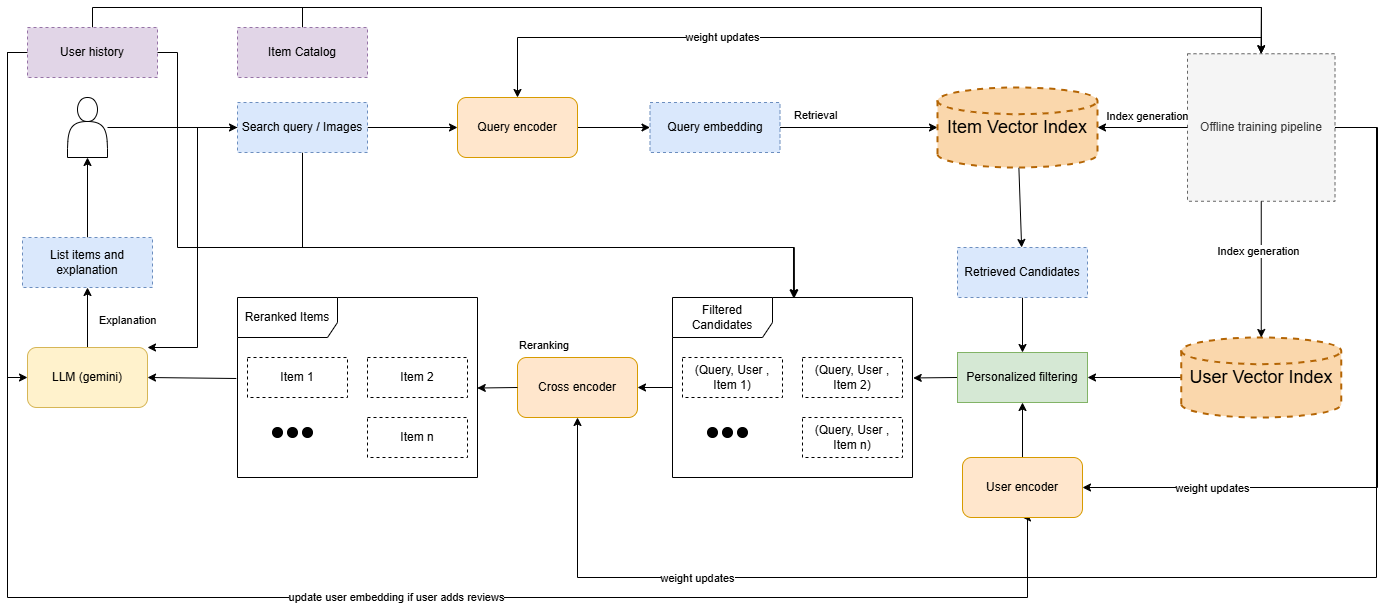
\includegraphics[width=1\textwidth]{Images/retrieval.png}
    \vspace{0.5cm}
    \caption{Quá trình Truy xuất sản phẩm}
    \label{fig:retrieval}
\end{figure}

Quy trình tìm kiếm bắt đầu khi người dùng thực hiện một truy vấn chủ động thông qua văn bản hoặc hình ảnh. Dữ liệu đầu vào này được chuyển đến bộ Query Encoders để thực hiện quá trình vector hóa. Tại đây, truy vấn thô được chuyển đổi thành vector nhúng (Query Embedding) nằm trong cùng không gian chiều với các vector sản phẩm đã được lập chỉ mục trước đó. Hệ thống sau đó sử dụng vector truy vấn này để quét qua Item Vector Index, thực hiện các phép toán tìm kiếm láng giềng gần nhất nhằm trích xuất ra tập hợp các ứng viên tiềm năng (Retrieved Candidates). Mục tiêu của giai đoạn này là tối ưu hóa độ phủ (Recall), đảm bảo thu thập được tất cả các sản phẩm có sự tương đồng về mặt ngữ nghĩa với ý định tìm kiếm của người dùng.

Điểm khác biệt của hệ thống so với các công cụ tìm kiếm truyền thống nằm ở cơ chế Personalized Filtering (Lọc cá nhân hóa). Song song với quá trình truy xuất dựa trên từ khóa, hệ thống đồng thời tham chiếu đến User Vector Index để trích xuất vector đặc trưng của người dùng—vốn được tổng hợp từ lịch sử hành vi và sở thích trong quá khứ. Vector người dùng này đóng vai trò như một bộ lọc ngữ cảnh, giúp điều chỉnh danh sách ứng viên ban đầu. Nhờ đó, các kết quả tìm kiếm không chỉ chính xác về mặt nội dung (ví dụ: đúng là "giày thể thao") mà còn phù hợp với gu thẩm mỹ riêng (ví dụ: ưu tiên "thương hiệu Nike" hay "phong cách tối giản") của từng cá nhân.

Tiếp theo, những ứng viên được lọc được đưa vào bộ Reranking để sắp xếp lại thứ hạng dựa vào query và lịch sử đánh giá của người dùng.

Sau khi danh sách ứng viên đã được sơ lọc, tập dữ liệu này được chuyển đến module LLM Reranking để thực hiện bước tinh chỉnh cuối cùng. Tại đây, một LLM sẽ phân tích sâu hơn mối quan hệ giữa truy vấn, chân dung người dùng và đặc điểm chi tiết của sản phẩm để sắp xếp lại thứ tự hiển thị. Quá trình này giúp loại bỏ các kết quả nhiễu và đưa các sản phẩm phù hợp nhất lên vị trí ưu tiên. Cuối cùng, hệ thống trả về danh sách sản phẩm kèm theo lời giải thích (List Items and explanation), giúp người dùng hiểu rõ lý do tại sao sản phẩm được đề xuất, qua đó tăng cường tính minh bạch và độ tin cậy của trải nghiệm tìm kiếm.

\section{Xây dựng Tháp Sản phẩm}

Trọng tâm của các hệ thống gợi ý hiện đại nằm ở khả năng chuyển đổi dữ liệu đa phương thức phức tạp thành các vector biểu diễn trong không gian ẩn, nơi khoảng cách hình học giữa các vector phản ánh trực tiếp mức độ tương đồng về mặt ngữ nghĩa. Trong kiến trúc đề xuất, Tháp Sản phẩm được thiết kế để xử lý song song và mã hóa ba luồng dữ liệu đặc trưng từ tập dữ liệu Amazon Reviews.

Đối với luồng \textbf{dữ liệu văn bản}, thông tin đầu vào được tổng hợp từ bốn trường dữ liệu giàu ngữ nghĩa bao gồm tiêu đề, mô tả chi tiết, đặc tính và thông số kỹ thuật của sản phẩm. Khối dữ liệu phi cấu trúc này được mã hóa thông qua mô hình ngôn ngữ BERT, cho phép hệ thống nắm bắt sâu sắc các ngữ cảnh và mối quan hệ từ vựng phức tạp mà các phương pháp nhúng từ truyền thống không thể thực hiện được.

Song song với đó, luồng \textbf{dữ liệu thị giác} tận dụng các hình ảnh sản phẩm gốc ở độ phân giải cao từ trường dữ liệu hình ảnh. Hệ thống sử dụng kiến trúc Vision Transformer (ViT) làm bộ trích xuất đặc trưng, giúp chuyển đổi các tín hiệu thị giác thành các vector đặc trưng toàn cục mang tính phân biệt cao, bổ sung thông tin trực quan quan trọng cho việc nhận diện sản phẩm.

Cuối cùng, luồng \textbf{dữ liệu dạng bảng} bao gồm các thuộc tính cấu trúc định lượng như điểm đánh giá trung bình, số lượng phản hồi, cùng các thông tin định danh phân loại như danh mục chính, danh mục phụ và thông tin cửa hàng. Các đặc trưng này được xử lý bởi một mạng nơ-ron đa tầng (MLP), có nhiệm vụ học các tương tác phi tuyến tính giữa các thuộc tính số học và phân loại. Đầu ra từ ba nhánh xử lý độc lập nêu trên sau đó được đồng bộ hóa và đi qua một tầng hợp nhất (Fusion Layer) để tạo thành một vector biểu diễn duy nhất, định hình nên bản sắc toàn diện của sản phẩm trong không gian tìm kiếm.

\begin{figure}[H]
    \centering
    % Đảm bảo tên file ảnh đúng với file bạn đã upload
    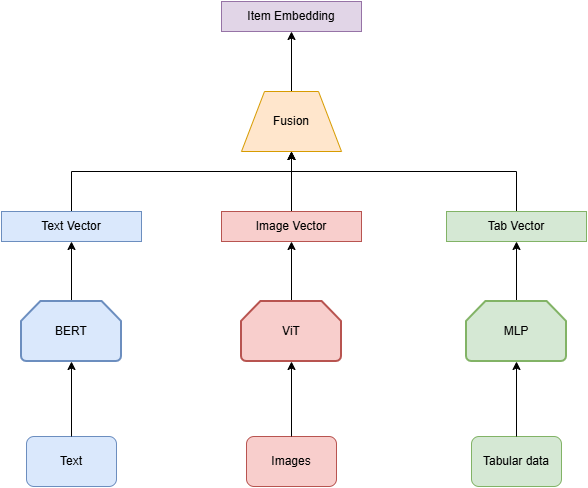
\includegraphics[width=0.8\textwidth]{Images/item_embedding.png} 
    \vspace{0.5cm}
    \caption{Kiến trúc Item Tower: Quy trình mã hóa và hợp nhất dữ liệu Đa phương thức}
    \label{fig:item_embedding}
\end{figure}

\subsection{Text Encoder: Mô-đun Mã hóa Văn bản}

TextEncoder là mô-đun mạng nơ-ron kế thừa từ \texttt{torch.nn.Module}, chịu trách nhiệm chuyển đổi dữ liệu văn bản thô (như tiêu đề, mô tả sản phẩm) thành các vector đặc trưng dày đặc (dense vectors). Đây là thành phần cốt lõi kiến tạo không gian biểu diễn ngôn ngữ cho toàn bộ kiến trúc tháp sản phẩm.

\textbf{1. Lựa chọn Mô hình và Chiến lược Huấn luyện}

Hệ thống tích hợp mô hình \texttt{all-mpnet-base-v2} làm mạng xương sống. Dựa trên bảng xếp hạng MTEB, kiến trúc MPNet thể hiện hiệu năng vượt trội trong phân khúc mô hình tầm trung \cite{6} đối với tác vụ tìm kiếm ngữ nghĩa, nhờ được huấn luyện trước trên hơn một tỷ cặp câu \cite{10}. 

Về chiến lược huấn luyện, hệ thống áp dụng cơ chế Trích xuất Đặc trưng (Feature Extraction) bằng cách đóng băng toàn bộ trọng số của khối MPNet thông qua \texttt{torch.no\_grad()}. Thiết kế này biến mô hình ngôn ngữ thành một bộ trích xuất tĩnh, giúp hệ thống tiết kiệm tối đa tài nguyên bộ nhớ GPU, đồng thời bảo toàn nguyên vẹn tri thức ngữ nghĩa gốc, tránh hiện tượng quên thảm khốc (catastrophic forgetting) khi huấn luyện trên miền dữ liệu thương mại điện tử mới.

\textbf{2. Luồng Xử lý Dữ liệu (Data Pipeline)}

Để đảm bảo hiệu năng, danh sách văn bản đầu vào được chia nhỏ thành các lô (mini-batches) và xử lý qua ba giai đoạn nối tiếp:

\begin{itemize}
    \item \textbf{Giai đoạn 1: Phân mảnh và Chuẩn bị ma trận chú ý (Tokenization):} Hệ thống sử dụng thuật toán WordPiece để phân rã câu thành các từ phụ (sub-words), giải quyết triệt để vấn đề từ vựng ngoài từ điển. Các chuỗi được đệm hoặc cắt bớt để đồng bộ chiều dài. Song song đó, một ma trận Mặt nạ chú ý được sinh ra, gán giá trị 1 cho token mang ngữ nghĩa và giá trị 0 cho token đệm, nhằm định tuyến chính xác sự tập trung của cơ chế Self-Attention.
    
    \item \textbf{Giai đoạn 2: Trích xuất đặc trưng và Masked Mean Pooling:} Chuỗi token được đưa qua khối MPNet tĩnh để sinh ra các vector ngữ cảnh. Nhằm tận dụng thông tin từ toàn bộ câu thay vì chỉ phụ thuộc vào token \texttt{[CLS]}, hệ thống áp dụng kỹ thuật Pooling trung bình có trọng số. Cụ thể, các vị trí token đệm bị triệt tiêu về 0, và vector đại diện cuối cùng được tính bằng trung bình cộng của các token thực:
    \begin{equation}
        e_{\text{pooled}} = \frac{\sum_{i=1}^{L} (h_i \cdot \text{mask}_i)}{\sum_{i=1}^{L} \text{mask}_i + \epsilon}
    \end{equation}
    Trong đó, $h_i$ là trạng thái ẩn của token thứ $i$, $\text{mask}_i$ là mặt nạ tương ứng, và $\epsilon$ là hằng số cực nhỏ ($10^{-9}$) nhằm duy trì độ ổn định số học.
    
    \item \textbf{Giai đoạn 3: Chiếu không gian và Chuẩn hóa:} Vector tổng hợp $e_{\text{pooled}}$ đi qua một tầng mạng tuyến tính (\texttt{nn.Linear}) để thực hiện phép nén không gian ẩn:
    \begin{equation}
        \mathbb{R}^{768} \rightarrow \mathbb{R}^{256}
    \end{equation}
    Phép biến đổi này đóng vai trò đồng bộ hóa kích thước đặc trưng văn bản với tháp người dùng và các luồng dữ liệu hình ảnh. Cuối cùng, vector đầu ra trải qua bước chuẩn hóa L2, đưa về dạng vector đơn vị nhằm tối ưu hóa cho hàm Contrastive Loss hoạt động dựa trên độ tương đồng Cosine.
\end{itemize}

\subsection{Image Encoder: Mô-đun Mã hóa Hình ảnh}

\texttt{ImageEncoder} chịu trách nhiệm chuyển đổi dữ liệu hình ảnh thô thành các vector đặc trưng nén. Đặc thù của sàn thương mại điện tử là một sản phẩm thường sở hữu nhiều biến thể hình ảnh (ảnh chính diện, góc cạnh, bao bì). Thay vì chọn ngẫu nhiên hoặc tính trung bình cộng đơn thuần, điểm nhấn thiết kế của mô-đun này là việc tích hợp cơ chế Gating thông minh nhằm tự động đánh giá và tổng hợp thông tin từ nhiều nguồn ảnh thành một đại diện duy nhất.

\vspace{0.3cm}
\noindent \textbf{1. Lựa chọn Mô hình và Chiến lược Huấn luyện}

Hệ thống sử dụng kiến trúc Vision Transformer (ViT), cụ thể là biến thể \texttt{vit\_base\_patch16\_224}. Mô hình này chia ảnh đầu vào thành các mảnh (\textit{patches}) kích thước $16 \times 16$ pixels để xử lý tuần tự, mang lại sự cân bằng tối ưu giữa độ chính xác và chi phí tài nguyên \cite{11}. 

Tương tự như mô đun ngôn ngữ, chiến lược Trích xuất Đặc trưng được áp dụng bằng cách đóng băng toàn bộ trọng số mạng nền (\texttt{requires\_grad = False}). Kỹ thuật này triệt tiêu chi phí tính toán gradient, đồng thời bảo toàn các đặc trưng thị giác cốt lõi đã được mạng ViT học từ tập ImageNet, tránh hiện tượng quên thảm khốc (\textit{catastrophic forgetting}).

\vspace{0.3cm}
\noindent \textbf{2. Luồng Xử lý Dữ liệu (Data Pipeline)}

\begin{figure}[H]
    \centering
    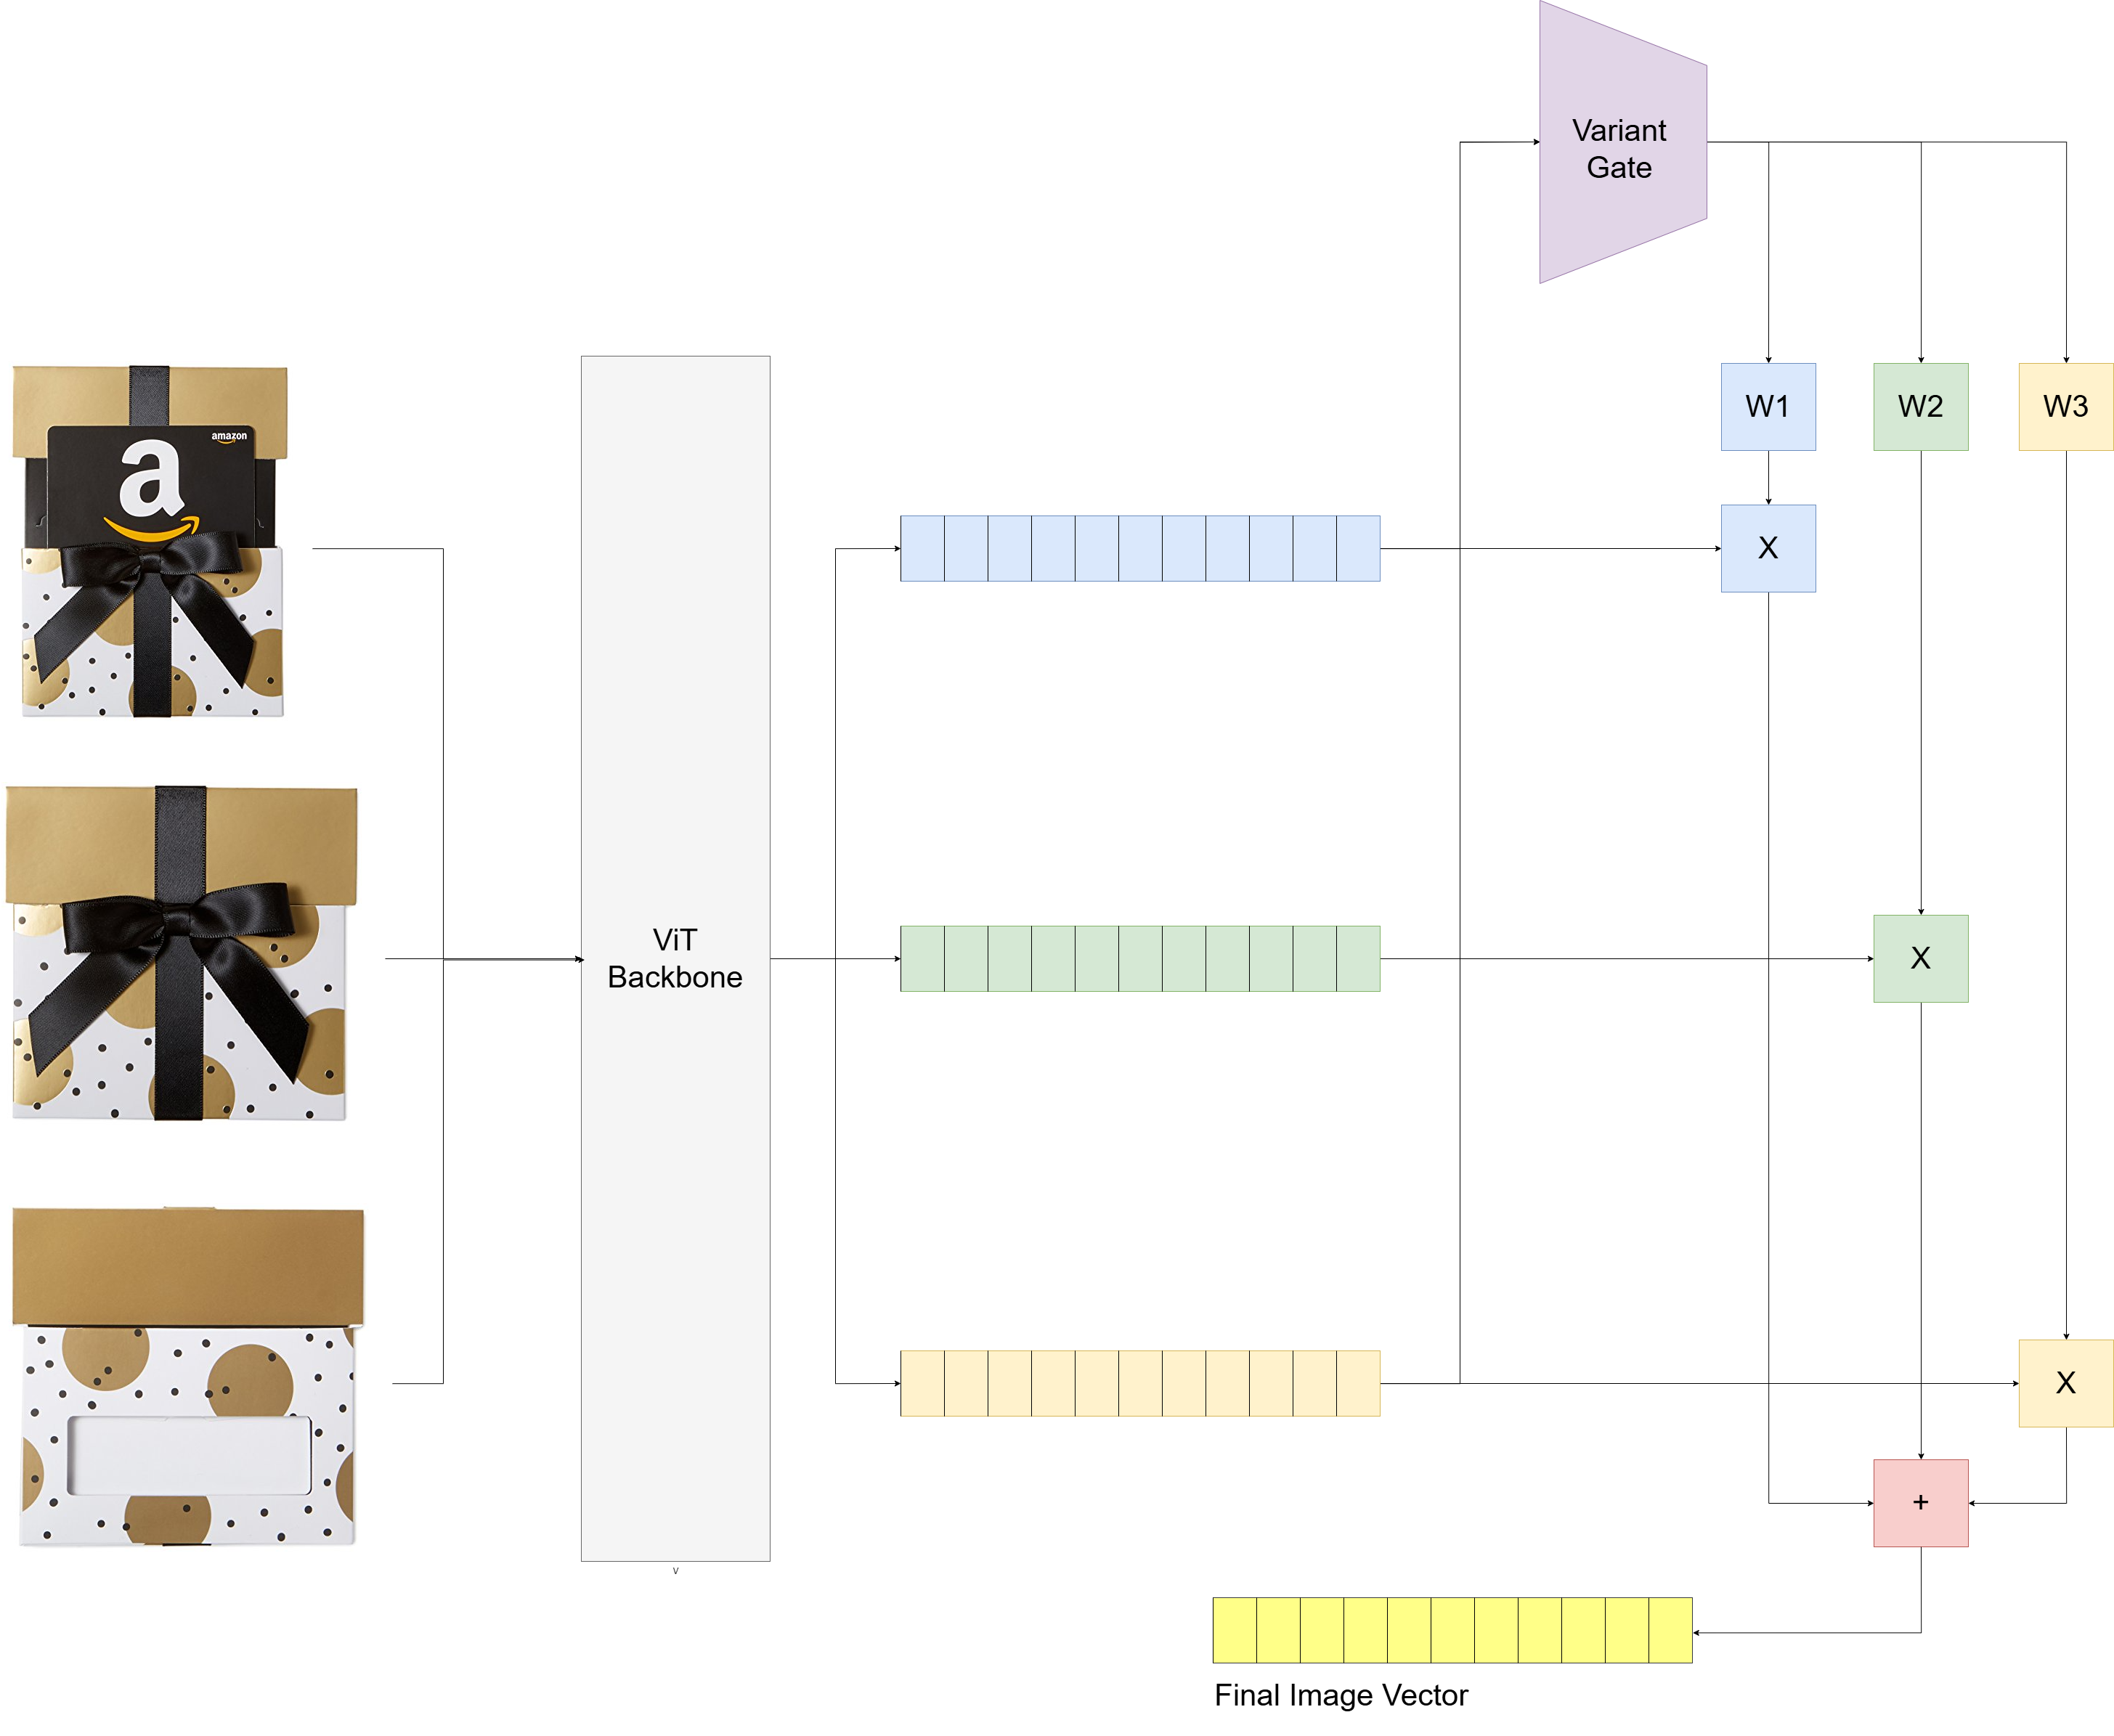
\includegraphics[width=0.8\textwidth]{Images/image_module.png} 
    \vspace{0.5cm}
    \caption{Quy trình Tính toán và Tổng hợp Đặc trưng Hình ảnh}
    \label{fig:image_module}
\end{figure}

Dựa trên sơ đồ kiến trúc tại Hình \ref{fig:image_module}, luồng xử lý hình ảnh được hiện thực hóa qua ba giai đoạn nối tiếp:

\begin{itemize}
    \item \textbf{Giai đoạn 1: Tiền xử lý (Preprocessing):} Nhằm đảm bảo tương thích với trọng số huấn luyện trước, mỗi hình ảnh được thay đổi kích thước về $224 \times 224$ pixels, chuyển đổi thành tensor \textit{Channel-first} trong khoảng $[0.0, 1.0]$, và cuối cùng được chuẩn hóa Z-score theo phân phối thống kê của tập ImageNet để đẩy nhanh tốc độ hội tụ.
    
    \item \textbf{Giai đoạn 2: Trích xuất đặc trưng và Chiếu không gian:} Các lô hình ảnh được đưa qua mô hình nền ViT tĩnh để sinh ra các vector đặc trưng thô. Ngay sau đó, một lớp tuyến tính (\texttt{self.proj}) thực hiện phép biến đổi không gian:
    \begin{equation}
        \mathbb{R}^{768} \rightarrow \mathbb{R}^{256}
    \end{equation}
    Phép nén này đồng bộ hóa hoàn toàn kích thước đặc trưng thị giác với tháp người dùng và luồng văn bản.
    
    \item \textbf{Giai đoạn 3: Tổng hợp đa ảnh và Chuẩn hóa:} Để xử lý bài toán không đồng nhất về số lượng biến thể ảnh, hệ thống áp dụng trực tiếp nguyên lý của Cơ chế Hợp nhất Không gian Vector đã được thiết lập lý thuyết tại Mục \ref{sec:attention_theory}. Luồng xử lý tại đây sử dụng một Cổng Biến thể đóng vai trò như mạng lưới sự chú ý để tự động học và phân bổ trọng số cho từng vector đặc trưng 256 chiều. Dựa trên bộ trọng số này, hệ thống thực hiện phép tính tổng có trọng số nhằm hội tụ các ảnh thành phần thành một vector đại diện duy nhất. Cơ chế này ép mô hình tự động điều hướng sự tập trung vào các bức ảnh sắc nét nhất mang tính đại diện cao và triệt tiêu tác động của ảnh nhiễu. Cuối cùng, hệ thống xử lý các vị trí khuyết dữ liệu đối với sản phẩm không có ảnh bằng cách điền ma trận không, đồng thời áp dụng chuẩn hóa L2 để xuất ra vector đặc trưng thị giác hoàn chỉnh, sẵn sàng cho khối hợp nhất đa phương thức phía sau.
    
\end{itemize}

\subsection{Tabular Encoder: Mô-đun Mã hóa Dữ liệu Bảng}

TabularEncoder chịu trách nhiệm mô hình hóa các thuộc tính siêu dữ liệu bao gồm điểm đánh giá và hệ thống phân loại. Mô-đun này được thiết kế theo luồng xử lý song song nhằm giải quyết hiệu quả bản chất hỗn hợp của dữ liệu bảng trước khi đồng bộ hóa không gian đặc trưng.

\vspace{0.3cm}
\noindent \textbf{1. Nhánh Xử lý Đặc trưng Phân loại}

Đối với các dữ liệu định danh rời rạc, hệ thống sử dụng các lớp mạng nhúng chuẩn \texttt{nn.Embedding} để ánh xạ chỉ số thành các vector đặc trưng không gian 32 chiều. Thiết kế bao gồm ba bảng nhúng độc lập phục vụ cho ba trường thông tin cốt lõi: Danh mục chính, Thương hiệu và Danh mục chi tiết. Riêng đối với trường Danh mục chi tiết mang đặc thù đa nhãn, một cơ chế tổng hợp nội bộ được áp dụng để tính toán ra một vector đại diện duy nhất cho toàn bộ tập hợp thẻ phân loại của sản phẩm.

\vspace{0.3cm}
\noindent \textbf{2. Nhánh Xử lý Đặc trưng Số thực}

Thay vì truyền trực tiếp dữ liệu thô vào lớp hợp nhất, hệ thống thiết lập một mạng nơ-ron đa tầng chuyên biệt để xử lý các thuộc tính định lượng như điểm đánh giá hay số lượt bình chọn hữu ích. Mạng nơ-ron này thực hiện chuỗi ba phép biến đổi liên tiếp: đầu tiên là phép chiếu mở rộng dữ liệu thô lên không gian ẩn 64 chiều, tiếp nối bằng hàm kích hoạt phi tuyến ReLU nhằm nắm bắt các tương quan không đơn điệu, và kết thúc bằng một lớp nén đưa dữ liệu về lại không gian mục tiêu 32 chiều. 

Sự thiết kế song song này đảm bảo toàn bộ đặc trưng định lượng và định danh đều được quy chuẩn về cùng một kích thước chiều, tạo điều kiện trơn tru nhất để nối ghép thành một vector dữ liệu bảng hoàn chỉnh, sẵn sàng tích hợp cùng đặc trưng văn bản và hình ảnh ở khối hợp nhất đa phương thức cuối cùng.

\vspace{0.3cm}
\noindent \textbf{3. Nhánh Hợp nhất Đặc trưng Bảng}

Tại tầng xử lý cuối cùng hay còn gọi là Lớp Hợp nhất, hệ thống thực hiện phép ghép nối chuỗi cho toàn bộ các vector đặc trưng phân loại và số thực đã qua tiền xử lý ở hai nhánh trên. Khối tensor tổng hợp này sau đó được truyền qua một mạng nơ-ron đa tầng để thực hiện ép kiểu và nén thông tin. Kết quả đầu ra là một vector đại diện duy nhất có kích thước không gian ẩn 256 chiều. Phép chiếu không gian ở giai đoạn cuối này đóng vai trò chốt chặn thiết yếu, đảm bảo đặc trưng siêu dữ liệu của sản phẩm được đồng bộ hoàn toàn về mặt kích thước với mô-đun văn bản và mô-đun hình ảnh, tạo tiền đề hoàn hảo cho giai đoạn dung hợp đa phương thức toàn cục.

\subsection{Cơ chế hợp nhất dữ liệu đa phương thức}

Đóng vai trò là thành phần chốt chặn cuối cùng trong kiến trúc Tháp Sản phẩm, cơ chế cổng hợp nhất chịu trách nhiệm tổng hợp các vector đặc trưng từ ba luồng dữ liệu riêng biệt: văn bản, hình ảnh và dữ liệu bảng. Dựa trên nền tảng lý thuyết về cơ chế chú ý đã được phân tích chi tiết tại \ref{sec:attention_theory}, đồ án tùy chỉnh module này để thực hiện phép hợp nhất có trọng số động. Cách tiếp cận này không chỉ giúp hệ thống tự động đánh giá mức độ đóng góp của từng phương thức dữ liệu đối với một mặt hàng cụ thể, mà còn cung cấp cơ chế xử lý linh hoạt cho thực trạng dữ liệu khuyết thiếu thường gặp trong môi trường thương mại điện tử.

\vspace{0.3cm}
\noindent \textbf{Tùy biến Mạng Gating dùng chung}

Thay vì sử dụng các mạng đánh giá độc lập, đồ án thiết kế một mạng Gating dùng chung cho toàn bộ các luồng dữ liệu nhằm đảm bảo sự công bằng và nhất quán trong thang đo. Kế thừa kiến trúc mạng truyền thẳng cơ sở, module này bao gồm một lớp tuyến tính nén phân nửa số chiều dữ liệu, kết hợp cùng hàm kích hoạt phi tuyến ReLU và một lớp đầu ra vô hướng. Điểm số vô hướng sinh ra đại diện cho mức độ tin cậy hay hàm lượng thông tin hữu ích mà mỗi nhánh dữ liệu mang lại cho bản sắc chung của sản phẩm.

\vspace{0.3cm}
\noindent \textbf{Quy trình tính toán và Xử lý khuyết thiếu}

Quy trình tính toán thực tế của đồ án được triển khai qua các bước tinh chỉnh chặt chẽ. Sau khi mạng Gating sinh ra các điểm số thô cho ba nhánh, hệ thống kích hoạt cơ chế xử lý ngoại lệ thông qua một ma trận mặt nạ. Ma trận này làm nhiệm vụ quét và phát hiện các luồng thông tin không tồn tại, chẳng hạn như sản phẩm thiếu ảnh minh họa, từ đó gán ngay một giá trị âm vô cùng xấp xỉ $-10^9$ cho điểm số tương ứng. Bước can thiệp kỹ thuật này đóng vai trò sống còn trước khi đưa dữ liệu qua hàm Softmax, đảm bảo trọng số phân bổ cho các thành phần bị khuyết sẽ tự động triệt tiêu về $0$, qua đó cách ly hoàn toàn xung nhiễu khỏi vector tổng hợp.

Sau bước lọc nhiễu, hệ thống áp dụng hàm Softmax để chuyển hóa các điểm số thô thành một phân phối xác suất có tổng bằng $1$. Trọng số động của luồng văn bản, hình ảnh và dữ liệu bảng lần lượt được xác định qua ma trận:
\begin{equation}
    \mathbf{W} = \text{Softmax}(\mathbf{G}) = [w_t, w_i, w_b]
\end{equation}

Vector hợp nhất cuối cùng $\mathbf{v}_{\text{fused}}$ được đồ án thiết lập dựa trên phép cộng có trọng số của các vector thành phần:
\begin{equation}
    \mathbf{v}_{\text{fused}} = w_t \cdot \mathbf{e}_{\text{text}} + w_i \cdot \mathbf{e}_{\text{img}} + w_b \cdot \mathbf{e}_{\text{tab}}
\end{equation}

Để hoàn thiện, kết quả này trải qua phép chuẩn hóa L2 nhằm đưa vector về độ dài đơn vị. Bước chuẩn hóa này tạo ra vector đại diện sản phẩm hoàn chỉnh, đảm bảo tính ổn định và tính đẳng hướng tối đa khi tham gia vào các phép tính toán độ tương đồng Cosine trong không gian truy xuất toàn cục phía sau.

\section{Xây dựng Tháp Người dùng}

\subsection{Tổng quan và Nền tảng Kỹ thuật}
Tháp người dùng đảm nhận vai trò mô hình hóa sở thích và hành vi của người dùng dựa trên lịch sử tương tác. Khác biệt với các phương pháp lọc cộng tác truyền thống vốn coi sở thích là yếu tố tĩnh, module này tiếp cận bài toán dưới góc độ Gợi ý Tuần tự (\textit{Sequential Recommendation}). Mục tiêu cốt lõi là học được một vector biểu diễn người dùng $\mathbf{u}_t$ tại thời điểm $t$, sao cho vector này bao hàm được ý định mua sắm tiếp theo dựa trên chuỗi $n$ tương tác quá khứ $S = \{i_1, i_2, \dots, i_t\}$, trong đó $i_k$ là sản phẩm mà người dùng đã tương tác tại bước thứ $k$.

Về mặt nền tảng kỹ thuật, hệ thống sử dụng kiến trúc Transformer Encoder lấy cảm hứng từ mô hình SASRec \cite{7}. Việc lựa chọn kiến trúc này cho phép mô hình vượt qua hạn chế của các mạng RNN hay CNN truyền thống trong việc nắm bắt các mối quan hệ phụ thuộc dài hạn, từ đó hiểu sâu hơn về sự chuyển dịch trong thị hiếu người dùng theo thời gian.

\subsection{Cơ chế Biểu diễn Người dùng}
Để kiến tạo không gian biểu diễn người dùng phong phú, hệ thống xử lý chuỗi dữ liệu đầu vào thu được từ giai đoạn tiền xử lý. Mỗi phần tử trong chuỗi này là một tổ hợp thông tin bao gồm nội dung nhận xét của người dùng về sản phẩm và vector đặc trưng $\mathbf{v}_{\text{item}}$ của chính sản phẩm đó. Để đồng bộ hóa dữ liệu văn bản phi cấu trúc vào không gian tính toán chung, nhóm thực hiện biến đổi các nhận xét thông qua bộ mã hóa chuyên biệt dưới đây.

\subsubsection{ReviewTextEncoder và Chiến lược Chia sẻ Trọng số}
Trong kiến trúc Tháp Người dùng, thành phần mã hóa văn bản chịu trách nhiệm chuyển đổi nội dung bình luận tổng hợp thành các vector đặc trưng ngữ nghĩa. Một đặc điểm kiến trúc quan trọng trong thiết kế của hệ thống là việc áp dụng cơ chế Chia sẻ Trọng số (\textit{Weight Sharing}). Cụ thể, bộ mã hóa văn bản trong Tháp Người dùng không được khởi tạo độc lập mà sử dụng chung kiến trúc mạng và toàn bộ bộ tham số đã được huấn luyện của bộ mã hóa trong Tháp Sản phẩm. Điều này đồng nghĩa với việc các văn bản đánh giá của người dùng và mô tả sản phẩm đều được xử lý qua cùng một mô hình ngôn ngữ tiền huấn luyện và cùng một lớp chiếu không gian.

Chiến lược chia sẻ trọng số này mang lại ba lợi ích kỹ thuật thiết yếu. Thứ nhất, nó đảm bảo sự đồng bộ tuyệt đối về không gian ngữ nghĩa, giúp các văn bản từ phía người dùng và sản phẩm được ánh xạ vào cùng một hệ quy chiếu vector, tạo điều kiện thuận lợi cho mô hình trong việc so sánh và tìm kiếm sự tương đồng giữa lời nhận xét và mô tả sản phẩm. Thứ hai, cơ chế này giúp tối ưu hóa tài nguyên tính toán bằng cách giảm đáng kể số lượng tham số cần lưu trữ, tránh việc hệ thống phải duy trì hai mô hình ngôn ngữ lớn riêng biệt. Cuối cùng, Tháp Người dùng có thể thừa hưởng trực tiếp khả năng hiểu ngôn ngữ đã được tinh chỉnh từ quá trình huấn luyện Tháp Sản phẩm, giúp quá trình hội tụ diễn ra nhanh hơn.

Về mặt cài đặt kỹ thuật, module này tiếp nhận đầu vào là danh sách các chuỗi văn bản đánh giá trong lịch sử hành vi và trả về một tensor có kích thước $[B, S, D_{\text{latent}}]$, tương ứng với kích thước lô, độ dài chuỗi lịch sử và kích thước vector đặc trưng $256$ chiều.

\subsubsection{ReviewTabularEncoder: Mô-đun Mã hóa Cấu trúc Đánh giá}
Mô-đun \texttt{ReviewTabularEncoder} chịu trách nhiệm mã hóa các thông tin định lượng và định danh gắn liền với bài đánh giá, bao gồm ba trường dữ liệu cốt lõi: điểm đánh giá (\textit{Rating}) trong thang đo $1-5$, số lượt bình chọn hữu ích (\textit{Helpful Votes}) và trạng thái xác thực mua hàng (\textit{Verified Purchase}). Mục tiêu của mô-đun là chuyển đổi các tín hiệu thô này thành một vector đặc trưng thống nhất, bổ sung ngữ cảnh tin cậy cho nội dung văn bản.

\vspace{0.3cm}
\noindent \textbf{Kiến trúc Mạng và Các Khối Xử lý}

Hệ thống được thiết kế với ba khối xử lý chuyên biệt tương ứng với đặc thù của từng loại dữ liệu. Đối với thuộc tính phân loại như trạng thái xác thực mua hàng, hệ thống sử dụng lớp \texttt{nn.Embedding} để chuyển đổi dữ liệu rời rạc sang không gian vector liên tục. Không gian nhúng được thiết lập với 3 trạng thái bao gồm giá trị đệm, đã mua và chưa xác thực, được ánh xạ vào vector có kích thước mặc định là $4$ chiều.

Đối với dữ liệu số học, một mạng Perceptron đa lớp (MLP) được thiết kế để biến đổi cặp giá trị điểm số và lượt bình chọn từ không gian 2 chiều sang không gian đặc trưng cao chiều hơn. Kiến trúc mạng bao gồm lớp ẩn $64$ chiều kết hợp với hàm kích hoạt ReLU, sau đó nén xuống $32$ chiều. Thiết kế này cho phép mô hình nắm bắt các tương tác phi tuyến tính phức tạp giữa điểm số và mức độ tin cậy của cộng đồng, ví dụ như sự khác biệt ngữ nghĩa giữa một đánh giá điểm thấp nhưng nhận được nhiều sự đồng tình so với một đánh giá điểm thấp nhưng ít được quan tâm.

Tại tầng xử lý cuối cùng, Khối Hợp nhất (\textit{Fusion Block}) chịu trách nhiệm tổng hợp thông tin từ nhánh số học $32$ chiều và nhánh phân loại $4$ chiều. Vector ghép nối có kích thước tổng thể là $36$ được đưa qua một mạng nơ-ron đa lớp để tạo ra đầu ra cuối cùng. Điểm đáng lưu ý trong thiết kế là lớp cuối cùng được cấu hình là lớp tuyến tính thuần túy không kèm hàm kích hoạt. Thiết kế này cho phép vector đầu ra nhận các giá trị thực trong toàn miền $(-\infty, +\infty)$, giúp bảo toàn sự phong phú của thông tin (\textit{information richness}) trước khi được tích hợp vào các lớp tiếp theo của Tháp Người dùng.

\vspace{0.3cm}
\noindent \textbf{Quy trình Xử lý Luồng Dữ liệu}

Quy trình xử lý diễn ra theo trình tự chặt chẽ nhằm đảm bảo tính toàn vẹn của dữ liệu. Đầu vào bao gồm điểm số, lượt bình chọn và trạng thái xác thực sau khi được làm sạch và chuẩn hóa sẽ được phân tách vào các nhánh xử lý tương ứng. Trạng thái xác thực đi qua lớp Embedding để tạo vector $\mathbf{v}_{\text{cat}}$, trong khi điểm số và lượt bình chọn đi qua mạng chiếu số học để tạo vector $\mathbf{v}_{\text{num}}$. Hai thành phần này sau đó được ghép nối thành vector tổng hợp $\mathbf{v}_{\text{concat}}$ theo công thức:
\begin{equation}
    \mathbf{v}_{\text{concat}} = [\mathbf{v}_{\text{num}}; \mathbf{v}_{\text{cat}}]
\end{equation}
Cuối cùng, vector tổng hợp được đưa qua mạng Fusion để tạo ra biểu diễn vector đầu ra, đại diện cho ngữ cảnh cấu trúc toàn diện của bài đánh giá.

\subsubsection{Cổng Hợp nhất Người dùng (User Fusion Gate)}

Cổng \texttt{GatingFusionLayer} đóng vai trò trung tâm trong việc tổng hợp vector biểu diễn tương tác của người dùng. Nhiệm vụ cốt lõi của thành phần này là kết hợp vector định danh sản phẩm $\mathbf{v}_{\text{item}}$ thu được từ Tháp Sản phẩm với ngữ cảnh tương tác cụ thể, bao gồm nội dung đánh giá $\mathbf{v}_{\text{text}}$ và các chỉ số định lượng $\mathbf{v}_{\text{tabular}}$. Mục tiêu là tạo ra một vector duy nhất $\mathbf{h}_{\text{seq}}$ đại diện cho một bước trong chuỗi hành vi thông qua cơ chế \textit{Gating}, cho phép mô hình tự động điều chỉnh mức độ đóng góp của từng nguồn thông tin dựa trên ngữ cảnh thực tế.

\vspace{0.3cm}
\noindent \textbf{Kiến trúc và Các Khối Xử lý}

Về mặt kiến trúc, module bao gồm hai khối xử lý song song. Khối Chiếu và Đồng bộ sử dụng ba lớp tuyến tính riêng biệt để đưa các vector đầu vào có kích thước khác nhau về cùng một không gian chiều chung $d_{\text{model}} = 256$, chuẩn bị cho quá trình cộng gộp. Song song đó, Mạng \textit{Gating} được thiết kế dưới dạng một mạng perceptron đa lớp ($\text{Linear} \to \text{ReLU} \to \text{Linear}$) tiếp nhận toàn bộ dữ liệu ghép nối đầu vào để tính toán điểm số tầm quan trọng cho từng thành phần Item, Text và Tabular.

\vspace{0.3cm}
\noindent \textbf{Quy trình Xử lý}

Quy trình xử lý diễn ra tuần tự qua ba bước. Đầu tiên, các vector đặc trưng được chiếu sang không gian chung và áp dụng hàm kích hoạt phi tuyến ReLU để tăng khả năng biểu diễn. Kế đến, hệ thống thực hiện tính toán trọng số thông qua hàm Softmax, tái sử dụng cơ chế hợp nhất động tương tự như đã trình bày tại phần Tháp Sản phẩm, nhưng áp dụng cho ngữ nghĩa kết hợp giữa sản phẩm và phản hồi người dùng. Kết quả đầu ra là một tensor có kích thước $[B, S, D_{\text{latent}}]$, sẵn sàng làm đầu vào cho mạng \textit{Transformer Encoder} để mô hình hóa chuỗi thời gian.

\subsubsection{Module Mã hóa Vị trí (Positional Encoding)}

Trong kiến trúc Tháp Người dùng, chuỗi hành vi lịch sử được xử lý thông qua mạng Transformer. Một đặc điểm cố hữu của cơ chế \textit{Self-Attention} là tính bất biến hoán vị, nghĩa là mô hình xử lý tập hợp đầu vào song song mà không tự nhận biết được thứ tự trước sau của các phần tử. Tuy nhiên, đối với bài toán gợi ý tuần tự, thứ tự tương tác đóng vai trò tối quan trọng, chẳng hạn như hành vi mua điện thoại thường mang tính tiền đề và diễn ra trước khi mua ốp lưng. Để khắc phục hạn chế này, module \texttt{PositionalEncoding} được thiết kế nhằm bổ sung thông tin về vị trí tương đối hoặc tuyệt đối vào các vector biểu diễn trước khi chúng được đưa vào các lớp Attention.

\vspace{0.3cm}
\noindent \textbf{Phương pháp Mã hóa Sinusoidal}

Hệ thống áp dụng phương pháp Mã hóa Sinusoidal cố định theo kiến trúc Transformer nguyên bản. Phương pháp này tận dụng các hàm lượng giác với tần số biến thiên để tạo ra một đặc trưng vị trí độc nhất cho mỗi bước thời gian.

% \begin{figure}[H]
%     \centering
%     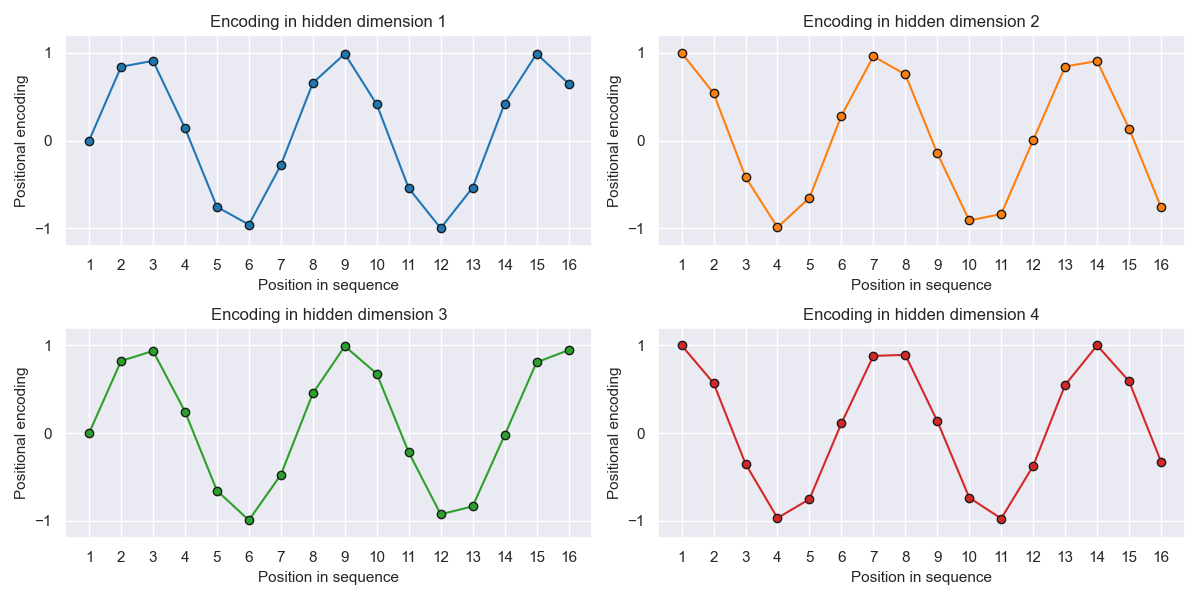
\includegraphics[width=1.0\textwidth]{Images/position_encoder.png}
%     \vspace{0.3cm}
%     \caption{Minh họa trực quan giá trị Positional Encoding trên 4 chiều ẩn đầu tiên. Các đường cong hình sin với tần số khác nhau giúp mô hình phân biệt vị trí trong chuỗi.}
%     \label{fig:pos_encoding_vis}
% \end{figure}


Dựa trên đề xuất của Vaswani và cộng sự \cite{12}, giá trị mã hóa tại vị trí $pos$ và chiều $i$ trong không gian vector kích thước $d_{\text{model}}$ được xác định bởi công thức toán học sau:
\begin{align}
    \text{PE}_{(pos, 2i)} &= \sin\left(\frac{pos}{10000^{2i/d_{\text{model}}}}\right) \\
    \text{PE}_{(pos, 2i+1)} &= \cos\left(\frac{pos}{10000^{2i/d_{\text{model}}}}\right)
\end{align}
Trong đó, các chiều chẵn $2i$ được áp dụng hàm Sine và các chiều lẻ $2i+1$ được áp dụng hàm Cosine. Việc kết hợp hai hàm lượng giác này cho phép mô hình lan truyền và ngoại suy thông tin vị trí một cách hiệu quả ngay cả đối với các chuỗi dài hơn độ dài đã gặp trong quá trình huấn luyện.

\noindent \textbf{Chi tiết Kỹ thuật và Quy trình Cài đặt}

Mô-đun được hiện thực hóa dưới dạng một lớp kế thừa từ \texttt{nn.Module} với quy trình xử lý được tối ưu hóa ngay từ bước khởi tạo. Cụ thể, một ma trận vị trí \texttt{pe} có kích thước $[\texttt{max\_len}, 1, d_{\text{model}}]$ được tính toán trước và lưu trữ vào bộ nhớ đệm thông qua cơ chế \texttt{register\_buffer}. Kỹ thuật này cho phép hệ thống ghi nhận ma trận như một phần trạng thái bền vững của mô hình nhưng không tham gia vào quá trình cập nhật gradient, giúp cố định thông tin vị trí và giảm tải số lượng tham số cần tối ưu.

Trong quá trình lan truyền xuôi, các vector vị trí tương ứng được cộng trực tiếp vào vector đặc trưng đầu vào theo công thức:
\begin{equation}
    \mathbf{x} = \mathbf{x} + \mathbf{PE}[:\texttt{x.size(0)}]
\end{equation}
Phép toán cộng tuyến tính này đóng vai trò quyết định giúp cơ chế \textit{Attention} phân biệt được các thực thể giống nhau nhưng xuất hiện tại các thời điểm khác nhau trong chuỗi hành vi, đảm bảo tính thứ tự của dữ liệu. Nhằm tăng cường khả năng tổng quát hóa, một lớp \texttt{Dropout} với tỷ lệ mặc định $0.1$ được áp dụng ngay sau bước cộng mã hóa. Thao tác này giúp ngăn chặn hiện tượng quá khớp bằng cách buộc mô hình học các mẫu cấu trúc tổng quát thay vì phụ thuộc thái quá vào thông tin vị trí tuyệt đối.

Trong ngữ cảnh cụ thể của hệ thống gợi ý, thành phần này nắm giữ vai trò then chốt trong việc mô hình hóa tính gần đây và nguyên tắc nhân quả. Nó cung cấp cơ sở tham chiếu để mô hình nhận thức được khoảng cách thời gian giữa các tương tác, từ đó tạo điều kiện cho cơ chế \textit{Self-Attention} phân bổ trọng số hợp lý: ưu tiên cao hơn cho các hành vi gần đây đại diện cho sở thích ngắn hạn, đồng thời vẫn duy trì ngữ cảnh dài hạn để đảm bảo độ chính xác trong việc dự báo hành động tiếp theo.

\subsubsection{Cơ chế Tạo và Tổng hợp Vector Người dùng}

Nhiệm vụ cốt lõi của phân hệ này là thực hiện chuyển đổi chuỗi các trạng thái ẩn tuần tự — vốn là đầu ra từ mạng \textit{Transformer} — thành một vector duy nhất đại diện cho chân dung sở thích toàn diện của người dùng. Quy trình này được xây dựng dựa trên sự kết hợp chặt chẽ giữa kỹ thuật mô hình hóa chuỗi thời gian và các phương pháp tổng hợp thông tin có chọn lọc.

\noindent \textbf{Quy trình Xử lý và Tổng hợp Vector Người dùng}

\begin{figure}[H]
    \centering
    
\includegraphics[width=0.95\linewidth]{images/user_tower.png} 
    \vspace{0.5cm}
    \caption{Kiến trúc chi tiết Tháp Người dùng với cơ chế mô hình hóa chuỗi đa phương thức.}
    \label{fig:user_tower_arch}
\end{figure}

Sơ đồ minh họa luồng xử lý dữ liệu tuần tự bên trong Tháp Người dùng, được thiết kế để chuyển đổi lịch sử hành vi phức tạp thành một vector đại diện sở thích duy nhất. Quá trình này diễn ra qua bốn giai đoạn xử lý phân tầng từ dưới lên trên:

\begin{itemize}
    \item \textbf{1. Tầng Mã hóa Đặc trưng Chia sẻ (\textit{Shared Encoders Layer}):} \\
    Tại mỗi bước thời gian trong chuỗi hành vi, hệ thống tiếp nhận bộ ba dữ liệu đầu vào gồm nội dung văn bản đánh giá, thông tin bảng số liệu và định danh sản phẩm. Các luồng dữ liệu này được đưa qua khối các bộ mã hóa chuyên biệt (\textit{Encoders}). Điểm đặc biệt trong thiết kế này là cơ chế chia sẻ trọng số (\textit{Share weight}), nghĩa là cùng một bộ tham số mã hóa được sử dụng lặp lại cho mọi bước thời gian và đồng bộ hoàn toàn với các bộ mã hóa tại Tháp Sản phẩm. Điều này đảm bảo tính nhất quán về không gian đặc trưng giữa hai tháp mô hình.

    \item \textbf{2. Tầng Hợp nhất Cục bộ (\textit{Fusion Gate}):} \\
    Sau khi trích xuất đặc trưng sơ cấp, tại mỗi bước thời gian, các vector thành phần được đưa qua cổng hợp nhất \textit{Fusion Gate}. Module này chịu trách nhiệm tổng hợp ba nguồn thông tin không đồng nhất thành một vector đại diện duy nhất (\textit{Vector Review}), gói gọn toàn bộ ngữ cảnh tương tác của người dùng tại thời điểm đó.

    \item \textbf{3. Tầng Mô hình hóa Tuần tự (\textit{Sequence Modeling Layer}):} \\
    Để mô hình nhận thức được thứ tự của các hành vi, giải thuật Mã hóa Vị trí (\textit{Positional Encoding}) được cộng trực tiếp vào các vector đặc trưng. Chuỗi vector sau khi đã tích hợp thông tin vị trí được đưa vào khối \textit{Transformer Encoder Block}. Tại đây, cơ chế \textit{Self-Attention} cho phép mô hình học các mối quan hệ phụ thuộc dài hạn và nắm bắt sự chuyển dịch trong thị hiếu người dùng qua thời gian.
\end{itemize}

Giai đoạn tiếp theo tập trung vào việc Tổng hợp Đặc trưng. Do độ dài lịch sử hành vi của người dùng mang tính biến thiên, hệ thống áp dụng kỹ thuật \textit{Masked Mean Pooling} để nén toàn bộ chuỗi trạng thái ẩn từ Transformer thành một vector đại diện duy nhất. Để thực hiện điều này, mặt nạ đệm ban đầu được xử lý và mở rộng chiều tương thích với tensor dữ liệu, trong đó các vị trí chứa thông tin thực được gán trọng số $1$ và vị trí đệm nhận giá trị $0$. Hệ thống tiến hành nhân từng phần tử giữa đầu ra mô hình và mặt nạ trọng số nhằm triệt tiêu hoàn toàn các vector tại vị trí đệm về vector $\mathbf{0}$, sau đó cộng dồn các đặc trưng dọc theo trục thời gian. Vector đại diện cuối cùng được xác định bằng cách chia tổng thu được cho số lượng hành vi thực tế, với việc bổ sung một hằng số nhỏ $\epsilon$ vào mẫu số để đảm bảo tính ổn định số học:
\begin{equation}
    \mathbf{u}_{\text{pooled}} = \frac{\sum_{t=1}^{T} (\mathbf{h}_t \cdot m_t)}{\sum_{t=1}^{T} m_t + \epsilon}
\end{equation}
Trong đó $\mathbf{h}_t$ là trạng thái ẩn tại bước $t$ và $m_t$ là giá trị mặt nạ nhị phân.

\vspace{0.2cm}

Quy trình khép lại bằng giai đoạn Tinh chỉnh và Chuẩn hóa. Vector trung bình sau khi tính toán được đưa qua một lớp Tuyến tính cuối cùng đóng vai trò như bộ chuyển đổi đặc trưng cao cấp, tối ưu hóa cho việc so khớp với sản phẩm. Đầu ra cuối cùng trải qua phép chuẩn hóa L2 để đưa về độ dài đơn vị trên mặt cầu, đảm bảo khoảng cách giữa người dùng và sản phẩm được đo lường chính xác và nhất quán thông qua độ tương đồng Cosine.

\section{Chiến lược Huấn luyện Hai giai đoạn}

Việc tối ưu hóa đồng thời các hàm mất mát tương phản nội bộ tháp sản phẩm và toàn cục giữa hai tháp trong một đồ thị tính toán duy nhất thường dẫn đến hiện tượng xung đột đạo hàm, đồng thời tiêu tốn lượng lớn tài nguyên bộ nhớ VRAM. Để khắc phục thách thức này và đảm bảo mô hình hội tụ ổn định, đồ án đề xuất áp dụng chiến lược huấn luyện hai giai đoạn. Quá trình này tách biệt việc thấu hiểu nội dung sản phẩm và việc nắm bắt hành vi người dùng thành hai bước tuần tự

\subsection{Giai đoạn 1: Tiền huấn luyện độc lập Tháp Sản phẩm}

Trong giai đoạn đầu tiên, để ngăn chặn tín hiệu nhiễu từ chuỗi lịch sử tương tác, cấu trúc Tháp Người dùng bị loại bỏ hoàn toàn khỏi đồ thị tính toán. Hệ thống chỉ tập trung cấp phát tài nguyên phần cứng để tối ưu hóa mạng nơ-ron của Tháp Sản phẩm. Đồ án sử dụng kho dữ liệu sản phẩm tĩnh bao gồm hình ảnh, văn bản mô tả và các thuộc tính dạng bảng làm tập dữ liệu huấn luyện.

Thành phần cốt lõi trong chiến lược tối ưu hóa của hệ thống là hàm mất mát dựa trên nguyên lý Học tương phản. Cụ thể, đồ án áp dụng biến thể \textit{Symmetric InfoNCE Loss}, phương pháp đã chứng minh hiệu quả vượt trội qua sự thành công của mô hình CLIP \cite{13}. Khác với các hàm mất mát truyền thống, phương pháp này thực hiện tính toán độ tương đồng chéo giữa các cặp dữ liệu đa phương thức theo cả hai chiều nhằm đồng bộ hóa không gian biểu diễn chung. Mục tiêu tối thượng là tối ưu hóa không gian vector sao cho các cặp dữ liệu tương ứng như hình ảnh và văn bản của cùng một sản phẩm sẽ có vector biểu diễn gần nhau do lực hút, trong khi các cặp dữ liệu không tương ứng bị đẩy ra xa nhau do lực đẩy.

Mặc dù hàm mất mát \textit{InfoNCE} thể hiện sự ưu việt trong việc đồng bộ hóa không gian biểu diễn toàn cục, nó vẫn bộc lộ hạn chế khi xử lý các tập dữ liệu có độ hạt mịn (fine-grained) và độ tương đồng nội nhóm cao, điển hình như miền dữ liệu Amazon Beauty. Trong không gian này, các mặt hàng thường có sự chồng chéo lớn về đặc trưng (ví dụ: các sản phẩm mỹ phẩm cùng chủng loại nhưng khác thương hiệu). Hàm \textit{InfoNCE} có xu hướng phân bổ lực đẩy đồng đều lên mọi mẫu âm tính trong lô, dẫn đến việc thiếu sự tập trung cần thiết để phân tách các sản phẩm cực kỳ giống nhau.

Để khắc phục hạn chế của hàm mất mát InfoNCE khi xử lý các tập dữ liệu có độ tương đồng nội nhóm cao, đồ án tích hợp thêm hàm Batch-Hard Triplet Loss vào giai đoạn tinh chỉnh. Thay vì dàn trải lực tối ưu đồng đều, phương pháp này chỉ tập trung xử lý mẫu đối nghịch khó nhất, tức là sản phẩm nhiễu có vị trí gần với mục tiêu nhất trong không gian vector. Dựa trên ma trận tương đồng Cosine giữa hai tập hợp biểu diễn, mô hình thiết lập một ranh giới an toàn $m$ nhằm ép buộc độ tương đồng của cặp dữ liệu mục tiêu phải luôn vượt trội hơn mẫu âm tính khó nhất một khoảng tối thiểu bằng $m$. Quá trình này được tính toán đối xứng theo cả hai chiều để đảm bảo tính đồng nhất của kiến trúc Hai tháp. Sự kết hợp giữa khả năng quy hoạch không gian toàn cục của InfoNCE và khả năng tinh chỉnh chi tiết cục bộ của Batch-Hard Triplet Loss giúp hệ thống xây dựng một không gian nhúng mạnh mẽ, qua đó phân biệt chính xác các mặt hàng có đặc điểm cực kỳ giống nhau trong những miền dữ liệu phức tạp.

\noindent \textbf{Vai trò chiến lược trong hệ thống gợi ý}

Trong kiến trúc đa phương thức của đề tài, hàm mất mát tương phản đóng vai trò then chốt trong việc định hình không gian biểu diễn. Chức năng quan trọng nhất của nó là đồng bộ hóa không gian vector, hoạt động như một lực hấp dẫn để kéo các biểu diễn đặc trưng từ các nguồn dữ liệu phân tán như văn bản, hình ảnh và dữ liệu bảng về cùng một không gian ngữ nghĩa thống nhất. Bên cạnh đó, thông qua việc phân biệt rõ ràng giữa các cặp tương ứng và không tương ứng trong lô dữ liệu, mô hình học được khả năng trích xuất các đặc trưng độc đáo mang tính phân biệt cao. Đây là tiền đề quan trọng giúp tối ưu hóa khả năng truy xuất ứng viên, nâng cao độ chính xác trong việc tìm kiếm và gợi ý sản phẩm phù hợp.

\subsection{Giai đoạn 2: Tinh chỉnh toàn cục đa tháp}

\noindent \textbf{Cơ chế Mẫu âm tính kết hợp}

Hàm mất mát toàn cục được thiết kế dựa trên sự kết hợp giữa chiến lược lấy mẫu âm tính trong lô và cơ chế tiêm mẫu âm tính rõ ràng. Thông thường, hệ thống chỉ tận dụng các sản phẩm khác trong cùng một lô huấn luyện làm mẫu đối nghịch giả định, với rủi ro rằng người dùng có thể vẫn thích chúng nhưng chưa có cơ hội tương tác. Để tối ưu hóa không gian biểu diễn và tận dụng tối đa phản hồi thực tế, đồ án bổ sung thêm cho mỗi người dùng một vector đại diện cho sản phẩm mà họ đã trực tiếp đánh giá thấp.

Giả sử một lô huấn luyện có kích thước $N=3$. Khi xem xét người dùng thứ nhất $u_1$, sản phẩm $v_1^+$ ở cùng chỉ số index được coi là cặp dương tính. Các sản phẩm $v_2^+$ và $v_3^+$ tự động trở thành mẫu âm tính trong lô. Đặc biệt, một sản phẩm $v_1^-$ do chính $u_1$ đánh giá thấp được ghép thêm vào không gian đối nghịch, tạo ra một rào cản ngữ nghĩa mạnh mẽ. Cơ chế này được minh họa chi tiết tại Bảng \ref{tab:in_batch_negatives}.

\begin{table}[H]
    \centering
    \caption{Minh họa cơ chế lấy mẫu kết hợp với kích thước lô $N=3$}
    \label{tab:in_batch_negatives}
    \renewcommand{\arraystretch}{1.5}
    \footnotesize
    \begin{tabularx}{\textwidth}{|>{\centering\arraybackslash}m{2.5cm}|>{\centering\arraybackslash}X|>{\centering\arraybackslash}X|>{\centering\arraybackslash}X|>{\centering\arraybackslash}X|}
    \hline
    \textbf{Người dùng \textbackslash Sản phẩm} & \textbf{Sản phẩm 1 ($v_1^+$)} & \textbf{Sản phẩm 2 ($v_2^+$)} & \textbf{Sản phẩm 3 ($v_3^+$)} & \textbf{Mẫu đánh giá thấp ($v_i^-$)} \\ \hline
    \textbf{Người dùng 1 ($u_1$)} & \cellcolor{green!20}\textbf{Dương tính} & \cellcolor{red!10}Âm tính & \cellcolor{red!10}Âm tính & \cellcolor{gray!30}Âm tính rõ ràng ($v_1^-$) \\ \hline
    \textbf{Người dùng 2 ($u_2$)} & \cellcolor{red!10}Âm tính & \cellcolor{green!20}\textbf{Dương tính} & \cellcolor{red!10}Âm tính & \cellcolor{gray!30}Âm tính rõ ràng ($v_2^-$) \\ \hline
    \textbf{Người dùng 3 ($u_3$)} & \cellcolor{red!10}Âm tính & \cellcolor{red!10}Âm tính & \cellcolor{green!20}\textbf{Dương tính} & \cellcolor{gray!30}Âm tính rõ ràng ($v_3^-$) \\ \hline
    \end{tabularx}
\end{table}

\noindent \textbf{Quy trình Tính toán Toán học}

Quá trình tối ưu hóa diễn ra qua các bước tính toán tuần tự:

Đầu tiên, hệ thống xác lập ma trận tương đồng cơ sở từ tập vector người dùng $\mathbf{U}$ và tập vector sản phẩm mục tiêu $\mathbf{V}^+$ có cùng kích thước lô $N$. Mỗi phần tử của ma trận $\mathbf{S}$ kích thước $N \times N$ được tính bằng tích vô hướng và chuẩn hóa bởi tham số nhiệt độ $\tau$:
$$S_{i,j} = \frac{\mathbf{u}_i \cdot (\mathbf{v}_j^+)^T}{\tau}$$

Tham số $\tau$ đóng vai trò kiểm soát độ sắc nét của phân phối xác suất, giúp mô hình phân biệt tốt hơn các mẫu khó phân loại. Đồng thời, hệ thống tính toán riêng điểm số tương đồng giữa người dùng và sản phẩm họ đánh giá thấp:
$$E_i = \frac{\mathbf{u}_i \cdot (\mathbf{v}_i^-)^T}{\tau}$$

Tiếp theo, hệ thống thực hiện tính toán hàm mất mát theo hai chiều với sự bất đối xứng về mặt dữ liệu đối nghịch:

\noindent \textbf{Chiều từ người dùng đến sản phẩm:} Mục tiêu là hướng dẫn vector người dùng tìm đến đúng sản phẩm mục tiêu, đồng thời né tránh các sản phẩm của người khác trong lô và đặc biệt phải đẩy lùi sản phẩm bị đánh giá thấp. Không gian đối nghịch lúc này được mở rộng từ $N$ lên $N+1$. Hàm Cross-Entropy cho chiều này được công thức hóa như sau, với thành phần $\exp(E_i)$ đóng vai trò là hình phạt bổ sung dưới mẫu số:
$$\mathcal{L}_{\text{U} \rightarrow \text{I}} = - \frac{1}{N} \sum_{i=1}^N \log \frac{\exp(S_{i,i})}{\sum_{j=1}^N \exp(S_{i,j}) + \exp(E_i)}$$

\noindent \textbf{Chiều từ sản phẩm đến người dùng:} Để bảo toàn đặc tính phân cụm tự nhiên của phương pháp lọc cộng tác, chiều này không tích hợp tín hiệu âm tính rõ ràng. Các vector sản phẩm chỉ có nhiệm vụ tìm đúng người dùng đã tương tác với chúng giữa các tập hợp người dùng khác trong lô:
$$\mathcal{L}_{\text{I} \rightarrow \text{U}} = - \frac{1}{N} \sum_{i=1}^N \log \frac{\exp(S_{i,i})}{\sum_{j=1}^N \exp(S_{j,i})}$$

Cuối cùng, giá trị mất mát tổng thể $\mathcal{L}_{\text{Total}}$ là trung bình cộng của mất mát hai chiều này. Cải tiến này giúp hệ thống không chỉ nhạy bén trong việc gom cụm sở thích mà còn cực kỳ quyết liệt trong việc loại bỏ những ứng viên kém chất lượng ra khỏi không gian gợi ý.

\noindent \textbf{Vai trò chiến lược trong hệ thống gợi ý}

Trong kiến trúc Hai tháp, hàm mất mát tương phản đóng vai trò là xương sống toán học kết nối toàn bộ hệ thống. Khác với các phương pháp học sâu nguyên khối, kiến trúc đề xuất duy trì sự độc lập hoàn toàn giữa quá trình trích xuất chuỗi hành vi tại Tháp Người dùng và quá trình nội suy nội dung đa phương thức tại Tháp Sản phẩm. Hệ quả tất yếu là các vector đại diện sinh ra từ hai tháp này ban đầu tồn tại trong những không gian toán học hoàn toàn dị biệt. Sự can thiệp của cơ chế học tương phản giữa người dùng và sản phẩm đóng vai trò giải quyết triệt để sự phân ly này thông qua ba khía cạnh chiến lược:

Thứ nhất, hàm mất mát thiết lập một không gian nhúng chung cho toàn hệ thống. Thông qua cơ chế tối ưu hóa đối xứng, thuật toán ép buộc không gian sở thích của khách hàng và không gian đặc trưng của mặt hàng phải đồng bộ hóa với nhau. Phương pháp này hoạt động như một lực hấp dẫn, kéo vector thói quen mua sắm lại gần đúng với vector hình ảnh và mô tả của món đồ tương ứng. Quá trình này về bản chất là việc dạy cho hệ thống cách biên dịch mượt mà từ ngôn ngữ hành vi sang ngôn ngữ nội dung.

Thứ hai, phương pháp này tối ưu hóa trực tiếp cho bài toán truy xuất ứng viên siêu tốc. Khác với hàm mất mát phân loại truyền thống chỉ xuất ra điểm số xác suất tuyệt đối, học tương phản là đại diện tiêu biểu của nhóm học đo lường. Cơ chế này trực tiếp nhào nặn cấu trúc hình học của không gian thông qua lực hút các cặp dữ liệu tương ứng và lực đẩy các mẫu không liên quan. Việc không gian được quy hoạch rõ ràng và có tính phân cụm cao dựa trên khoảng cách hình học là điều kiện tiên quyết để thuật toán tìm kiếm lân cận gần nhất có thể hoạt động chính xác trên các cơ sở dữ liệu vector quy mô lớn.

Thứ ba, môi trường tương phản tạo ra sức mạnh phân biệt tương đối cực kỳ sắc bén. Việc đặt một sản phẩm mục tiêu vào giữa hàng loạt mẫu âm tính trong cùng một lô huấn luyện tạo ra một áp lực cạnh tranh khốc liệt. Mô hình không chỉ học cách nhận diện sản phẩm phù hợp một cách độc lập, mà còn buộc phải tinh chỉnh trọng số sao cho khoảng cách từ người dùng đến sản phẩm đích luôn ngắn hơn khoảng cách đến toàn bộ các mặt hàng nhiễu khác. Sức ép tối ưu hóa này buộc mạng lưới nơ-ron của cả hai tháp phải chắt lọc ra những đặc trưng mang tính định danh cao nhất, qua đó nâng cao độ chính xác tuyệt đối cho toàn bộ luồng gợi ý đa phương thức.


\section{Giai đoạn 2: Re-ranker}
\subsection{Kiến trúc tổng quan Reranker}

Trong lĩnh vực tìm kiếm thông tin, việc chỉ dựa vào độ phù hợp ngữ nghĩa giữa truy vấn và tài liệu thường không đáp ứng đủ nhu cầu đa dạng của người dùng. Ngược lại, việc áp dụng cá nhân hóa một cách cứng nhắc lại có nguy cơ làm giảm tính đa dạng của kết quả và khiến hệ thống trở nên thiếu minh bạch, khó kiểm soát. Từ đó, một bài toán cốt lõi được đặt ra là làm thế nào để kết hợp hài hòa giữa tín hiệu đối sánh ngữ nghĩa truyền thống và tín hiệu sở thích cá nhân, đồng thời cấp cho hệ thống khả năng tự động đánh giá và điều chỉnh mức độ cá nhân hóa tùy thuộc vào từng ngữ cảnh truy vấn cụ thể.

Để giải quyết triệt để vấn đề này, một kiến trúc xếp hạng lại (reranker) tổng hợp được đề xuất, hoạt động dựa trên cơ chế kết hợp giữa mô hình mã hóa chéo (Embedding Cross-Encoder) và bộ nhớ người dùng (User Memory). Cụ thể, điểm số đánh giá mức độ phù hợp của một tài liệu, ký hiệu là $s_d$, được xác định thông qua hàm $f_{Ret}(\mathcal{P}_u, q, d)$, trong đó q là câu truy vấn, d là tài liệu ứng viên được trích xuất từ danh sách của mô hình xếp hạng bước một, và $\mathcal{P}_u$ là hồ sơ lịch sử của người dùng. Kiến trúc này vận hành bằng cách tính toán hai nguồn điểm số độc lập nhưng bổ trợ cho nhau: điểm phù hợp ngữ nghĩa giữa truy vấn và tài liệu ($s_d^q$) được xuất ra từ mô hình Cross-Encoder ($f_{CE}$), và điểm phù hợp cá nhân hóa ($s_d^u$) được tính toán thông qua mô hình Memory Encoder ($f_{Mem}$). Thay vì cộng gộp một cách tuyến tính và cố định, hai giá trị này được dung hợp thông qua một mô hình trộn (Mixing Model), ký hiệu là $g_{Mix}$. Mô hình kết hợp này sinh ra một trọng số động w, cho phép tính toán điểm số xếp hạng cuối cùng theo phương trình:

$$s_d = w \cdot s_d^q + (1-w) \cdot s_d^u = w \cdot f_{CE}(q, d) + (1-w) \cdot f_{Mem}(\mathcal{P}_u, q, d)$$

\begin{figure}[htbp]
    \centering
    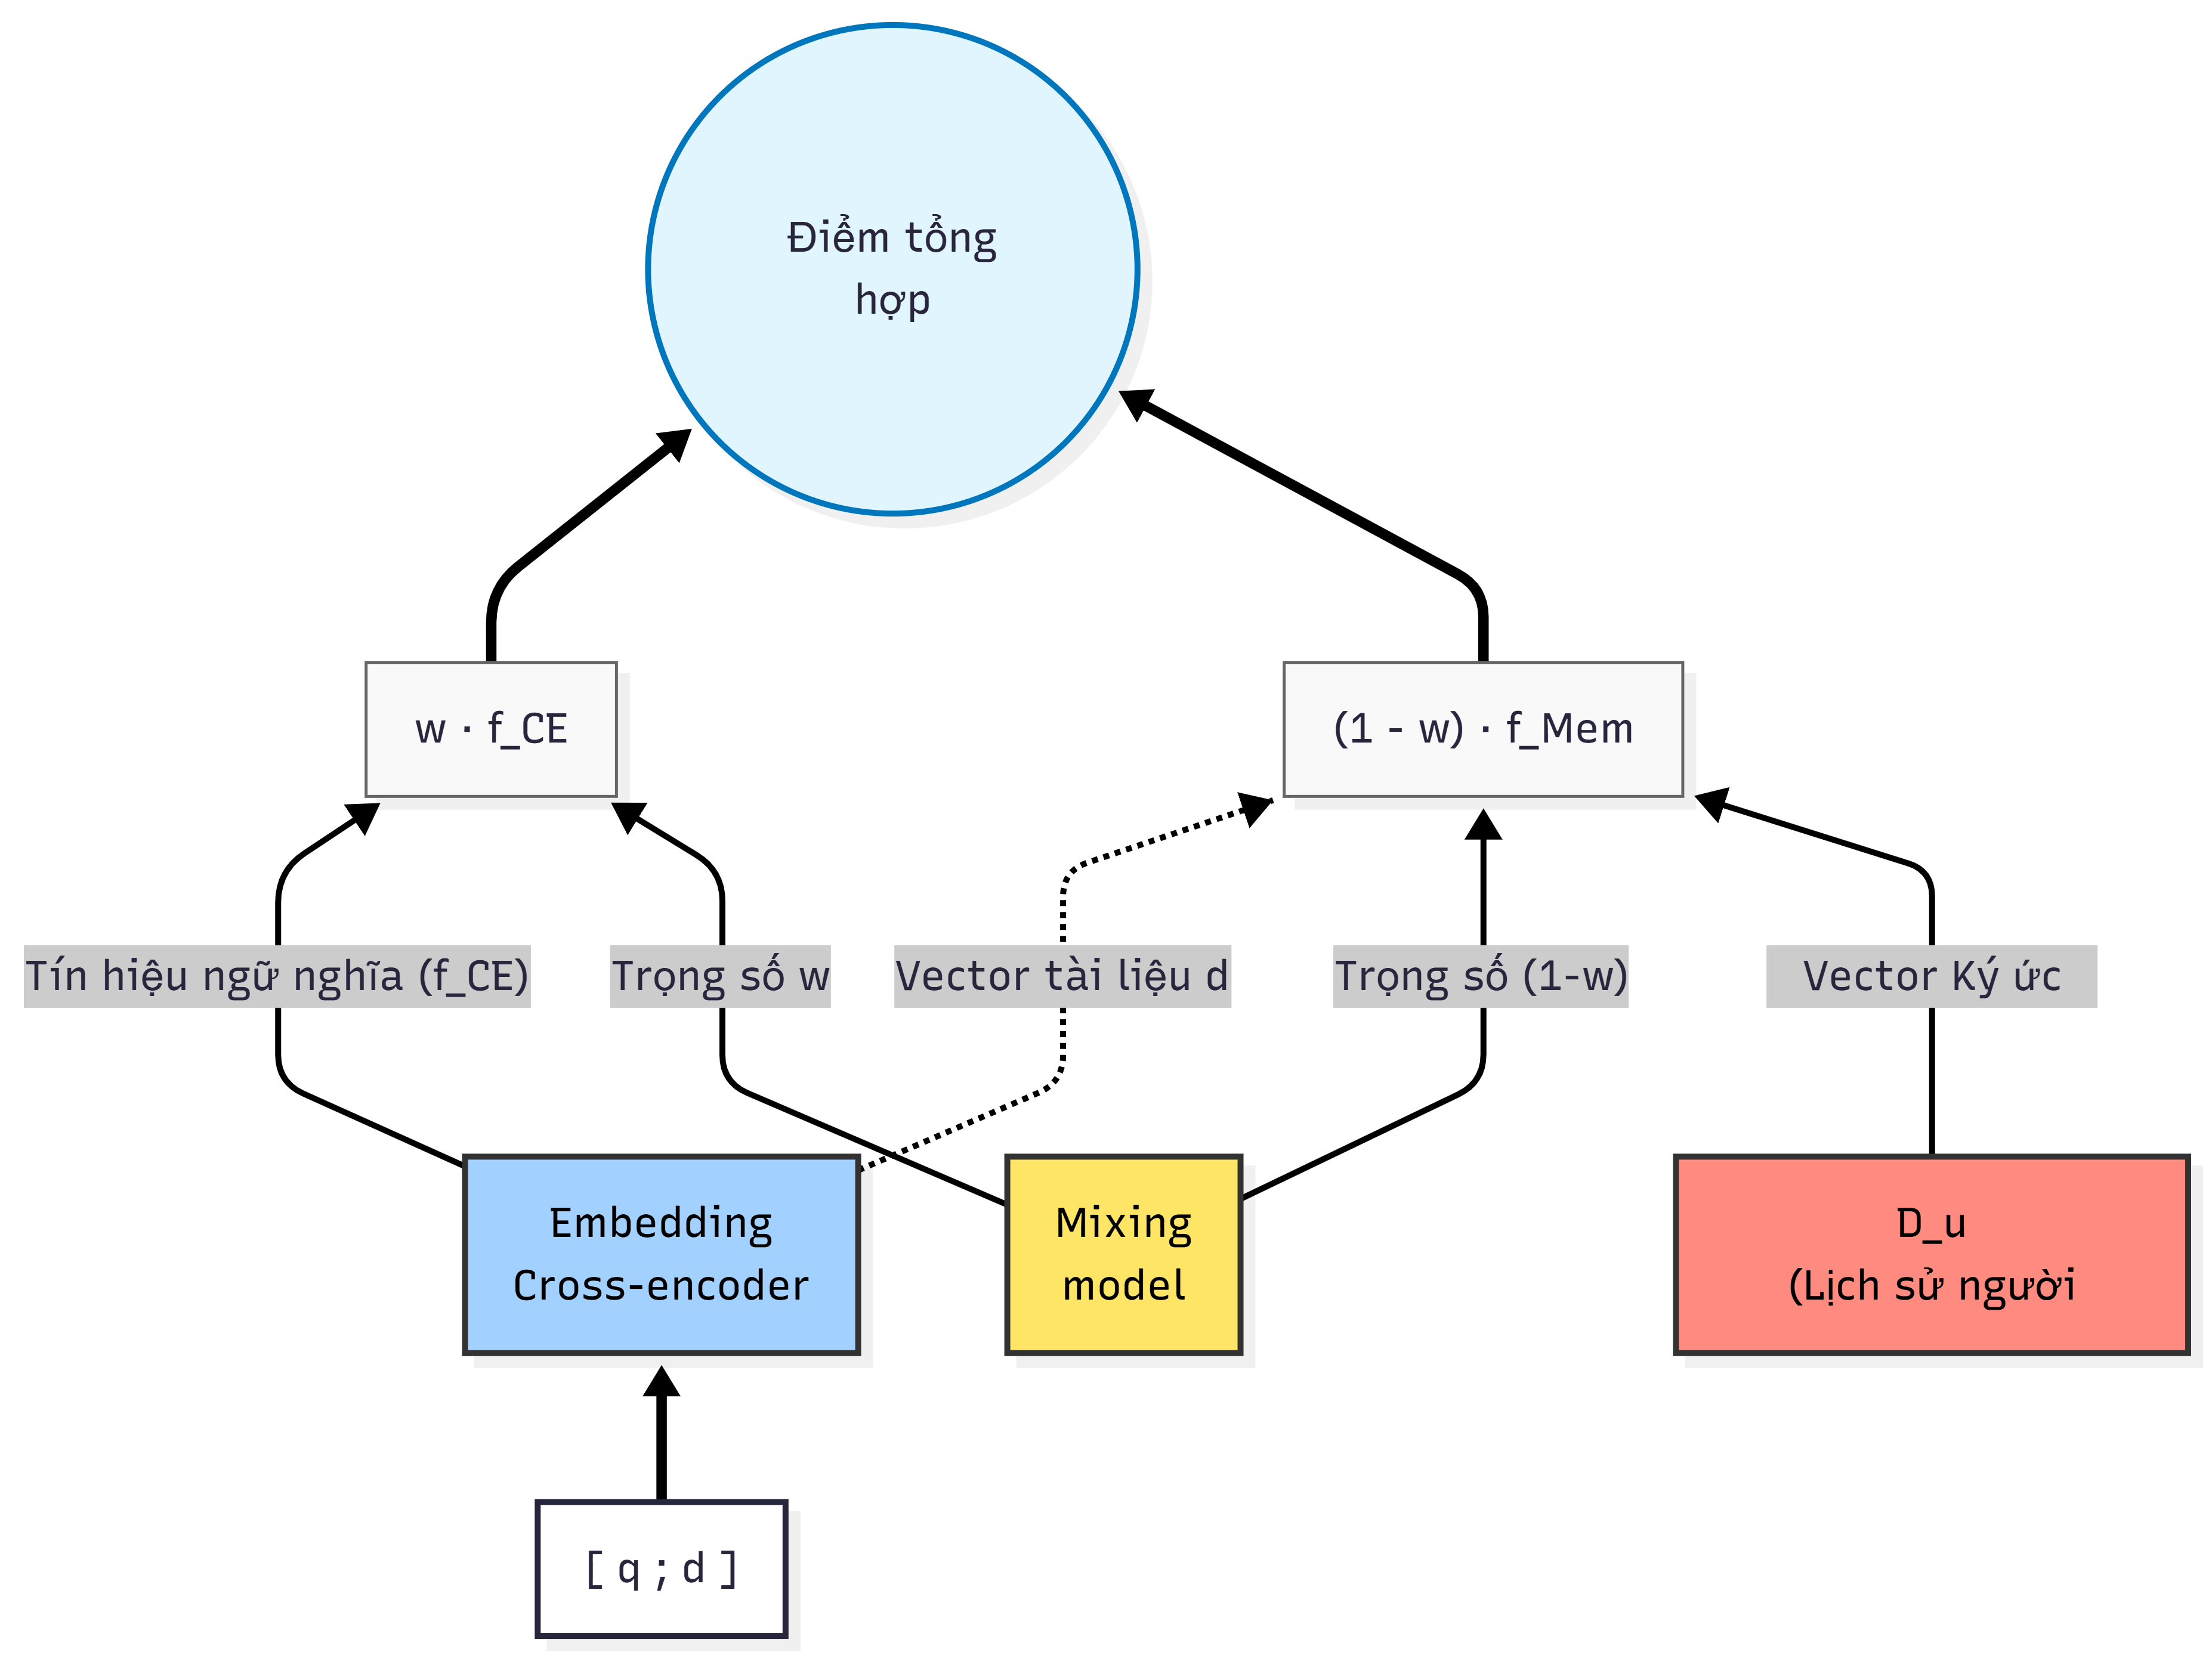
\includegraphics[width=0.85\textwidth]{Images/overview_cross_encoder.png} % Thay reranker_arch.png bằng tên file của bạn
    \vspace{0.5cm}
    \caption{Kiến trúc tổng quan của mô hình xếp hạng lại (Reranker) kết hợp đối sánh ngữ nghĩa và bộ nhớ cá nhân hóa.}
    \label{fig:reranker_arch}
\end{figure}

Sự khác biệt của kiến trúc này so với các mạng Cross-Encoder tiêu chuẩn nằm ở phương pháp biểu diễn đặc trưng. Các mô hình Cross-Encoder truyền thống thường gộp chung truy vấn và tài liệu thành một chuỗi thống nhất, làm hạn chế khả năng tách biệt và tái sử dụng đặc trưng của tài liệu cho các tác vụ khác. Ngược lại, mô hình đề xuất sử dụng kiến trúc Embedding Cross-Encoder, cho phép học các biểu diễn vector tách biệt nhưng vẫn chứa đựng thông tin ngữ cảnh chéo (cross-encoded) cho cả truy vấn ($\mathbf{q}$) và tài liệu ($\mathbf{d}$). Nhờ cấu trúc phân mảnh này, vector biểu diễn của tài liệu có thể trực tiếp tương tác với các vector đa chiều $V_i$ trong hồ sơ người dùng $\mathcal{P}_u$ thông qua thành phần $f_{Mem}$. Đồng thời, trọng số w được sinh ra đóng vai trò như một bộ dự báo hiệu suất, giúp hệ thống đánh giá mức độ tin cậy của tín hiệu từ Cross-Encoder, qua đó quyết định xem có cần sự can thiệp từ bộ nhớ cá nhân hay không. Cấu trúc phân tách điểm số này cũng cung cấp một cơ chế điều khiển thiết yếu, cho phép hệ thống dễ dàng quay về trạng thái không cá nhân hóa thông qua thao tác loại bỏ thành phần $s_d^u$ khỏi phương trình tính toán khi không cần thiết.

Tổng thể kiến trúc của giai đoạn xếp hạng lại được xây dựng theo dạng mô-đun nhằm cân bằng giữa việc phân tích ngữ nghĩa và khai thác thông tin cá nhân hóa. Cách tiếp cận này giúp hệ thống khắc phục được tính cứng nhắc của các phương pháp truyền thống, đồng thời cho phép kiểm soát linh hoạt mức độ can thiệp của dữ liệu lịch sử đối với từng truy vấn cụ thể. Thiết kế phân tách rõ ràng giữa các thành phần học ngữ nghĩa và thành phần trộn điểm cũng tạo nền tảng thuận lợi cho việc tối ưu hóa độc lập trong các quá trình huấn luyện tiếp theo.

\subsection{Embedding Cross Encoder}

Các kiến trúc Cross-Encoder tiêu chuẩn hiện đóng vai trò nền tảng trong nhiều hệ thống xếp hạng văn bản tiên tiến nhờ khả năng phân tích ngữ nghĩa sâu sắc và đánh giá mức độ liên quan với độ chính xác cao. Theo cách tiếp cận truyền thống, các mô hình này tiến hành ghép nối trực tiếp câu truy vấn và tài liệu ứng viên thành một chuỗi duy nhất thông qua các token phân cách, sau đó nạp toàn bộ chuỗi này qua các tầng tự chú ý (self-attention) của mô hình ngôn ngữ. Mặc dù phương pháp này tối ưu hóa được việc học các tương tác từ vựng chéo ở mức độ token (token-level cross-attention), nó lại bộc lộ một rào cản kiến trúc nghiêm trọng khi được tích hợp vào các hệ thống đòi hỏi tính cá nhân hóa. Nguyên nhân cốt lõi nằm ở việc các mô hình này thường nén toàn bộ thông tin của cặp truy vấn - tài liệu vào một token đại diện duy nhất (thường là token [CLS]) để tính toán ra một điểm số vô hướng cuối cùng. Sự hợp nhất này làm xóa nhòa ranh giới đặc trưng không gian của tài liệu. Khi không thể trích xuất được một biểu diễn vector độc lập đại diện cho tài liệu, hệ thống hoàn toàn thiếu đi cơ sở dữ liệu véc-tơ để tiếp tục đối chiếu với các nguồn thông tin khác, đặc biệt là không gian vector đa chiều chứa bộ nhớ về lịch sử tương tác của người dùng.

\begin{figure}[htbp]
    \centering
    % Dùng width=1\textwidth để ép hình ngang tràn viền lề, hiển thị to và rõ nhất
    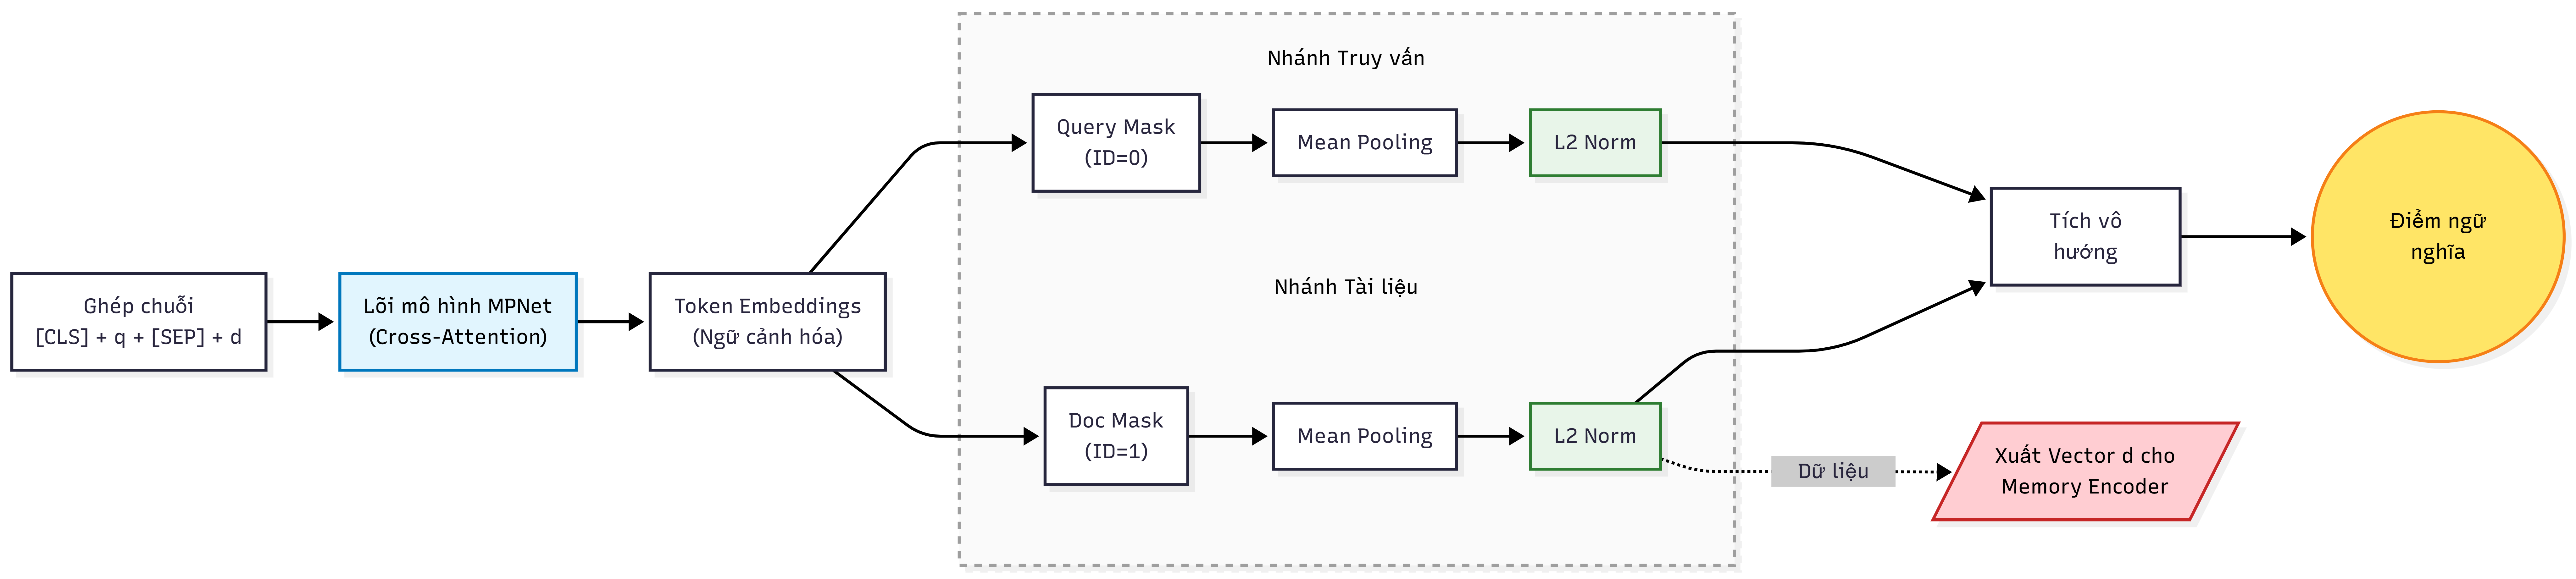
\includegraphics[width=1\textwidth]{Images/embedding_cross_encoder.png} % Thay embedding_ce.png bằng tên file của bạn
    \vspace{0.5cm}
    \caption{Sơ đồ luồng xử lý và trích xuất đặc trưng độc lập của kiến trúc Embedding Cross-Encoder.}
    \label{fig:embedding_ce}
\end{figure}

Để vượt qua giới hạn kiến trúc này, một cơ chế mang tên Embedding Cross-Encoder được triển khai, sử dụng mô hình ngôn ngữ MPNet làm lõi xử lý trung tâm. Lõi MPNet được ưu tiên lựa chọn nhờ khả năng nắm bắt ngữ nghĩa toàn cục vượt trội, bắt nguồn từ phương pháp huấn luyện kết hợp giữa cơ chế che giấu từ (masked language modeling) và hoán vị từ (permuted language modeling), giúp mô hình hiểu được cấu trúc ngữ cảnh phức tạp của các chuỗi văn bản dài. Quá trình xử lý của Embedding Cross-Encoder vẫn duy trì bước khởi đầu quen thuộc: nạp chuỗi ghép nối giữa truy vấn và tài liệu vào mô hình để trích xuất các biểu diễn token mang tính ngữ cảnh (contextualized token embeddings) từ tầng ẩn cuối cùng. Tuy nhiên, sự khác biệt mang tính đột phá nhằm giải quyết bài toán biểu diễn nằm ở bước phân tách đặc trưng. Thay vì sử dụng đầu ra từ token [CLS], hệ thống tận dụng các chuỗi định danh (sequence IDs) do bộ phân tách từ ngữ (tokenizer) cung cấp để xác định rõ ranh giới ngữ nghĩa. Dựa trên các định danh này, các ma trận mặt nạ (attention mask) chuyên biệt được tạo ra để định vị và cô lập chính xác tập hợp các token thuộc về câu truy vấn và tập hợp các token thuộc về tài liệu ứng viên. 

Ngay sau khi quá trình cô lập nhóm token hoàn tất, kỹ thuật gộp trung bình (mean pooling) được áp dụng một cách độc lập lên từng nhóm token tương ứng với mặt nạ phân bổ của chúng. Kết quả của phép toán này là sự hình thành của hai biểu diễn vector hoàn toàn tách biệt có cùng không gian số chiều: một vector đại diện cho truy vấn (q) và một vector đại diện cho tài liệu (d). Nhằm đảm bảo tính ổn định và đồng nhất trong hình học không gian vector, cả hai biểu diễn này đều tiếp tục trải qua quá trình chuẩn hóa L2 (L2 Normalization), đưa toàn bộ các giá trị về cùng một không gian độ đo chuẩn mực. Sau khi được chuẩn hóa, điểm số đánh giá mức độ phù hợp ngữ nghĩa cốt lõi giữa truy vấn và tài liệu được tính toán trực tiếp thông qua phép toán tích vô hướng của hai vector này. Nhờ sự hiện diện của bước chuẩn hóa trước đó, tích vô hướng ở công đoạn này mang ý nghĩa toán học tương đương với việc đo lường độ cosine similarity, phản ánh một cách trực quan và chính xác sự hội tụ về mặt ý nghĩa giữa ý định tìm kiếm của người dùng và nội dung cốt lõi của văn bản.

Nhìn chung, việc thiết kế và ứng dụng cơ chế Embedding Cross-Encoder mang lại những lợi ích mang tính bản lề cho toàn bộ kiến trúc của giai đoạn xếp hạng lại. Một mặt, kiến trúc này vẫn kế thừa trọn vẹn khả năng phân tích sự phụ thuộc từ vựng phức tạp nhờ cơ chế tự chú ý chéo diễn ra liên tục trong các tầng sâu của mô hình MPNet, qua đó bảo chứng cho độ chính xác cao của tín hiệu tìm kiếm ngữ nghĩa độc lập. Mặt khác, sự can thiệp mang tính cấu trúc ở lớp đầu ra đã giải phóng đặc trưng của tài liệu khỏi trạng thái nén cứng nhắc truyền thống. Vector tài liệu (d) được trích xuất ra mang một đặc tính lai độc đáo: nó vừa tồn tại như một thực thể toán học độc lập trong không gian vector, vừa chứa đựng dấu ấn ngữ cảnh sâu sắc từ sự tương tác trực tiếp với câu truy vấn. Chính biểu diễn tài liệu đã được ngữ cảnh hóa này sẽ đóng vai trò là đầu vào tiên quyết để thực hiện các phép toán đối chiếu chéo với bộ nhớ người dùng, kiến tạo nên tiền đề kỹ thuật vững chắc để hệ thống triển khai các thuật toán cá nhân hóa ở những giai đoạn tiếp theo một cách minh bạch và hiệu quả.


\subsection{Memory Encoder}

Sau khi trích xuất thành công vector biểu diễn tài liệu độc lập từ mô-đun Embedding Cross-Encoder, hệ thống tiến tới giai đoạn định lượng mức độ phù hợp của tài liệu ứng viên đối với từng người dùng cụ thể. Việc chỉ phụ thuộc vào câu truy vấn hiện tại sẽ bỏ qua nguồn thông tin ngữ cảnh có giá trị lớn ẩn chứa trong lịch sử tương tác. Tuy nhiên, lịch sử của một người dùng thường bao gồm một tập hợp nhiều sản phẩm hoặc tài liệu mang các chủ đề rất đa dạng. Do đó, việc đối chiếu trực tiếp một tài liệu mới với toàn bộ chuỗi sự kiện trong quá khứ đặt ra một thách thức lớn về mặt biểu diễn không gian. Hệ thống đòi hỏi một cơ chế tính toán chuyên biệt nhằm chuyển đổi dữ liệu lịch sử thô thành các tín hiệu cá nhân hóa có khả năng đo lường chính xác, mà không làm mất đi các sắc thái sở thích riêng biệt.

\begin{figure}[htbp]
    \centering
    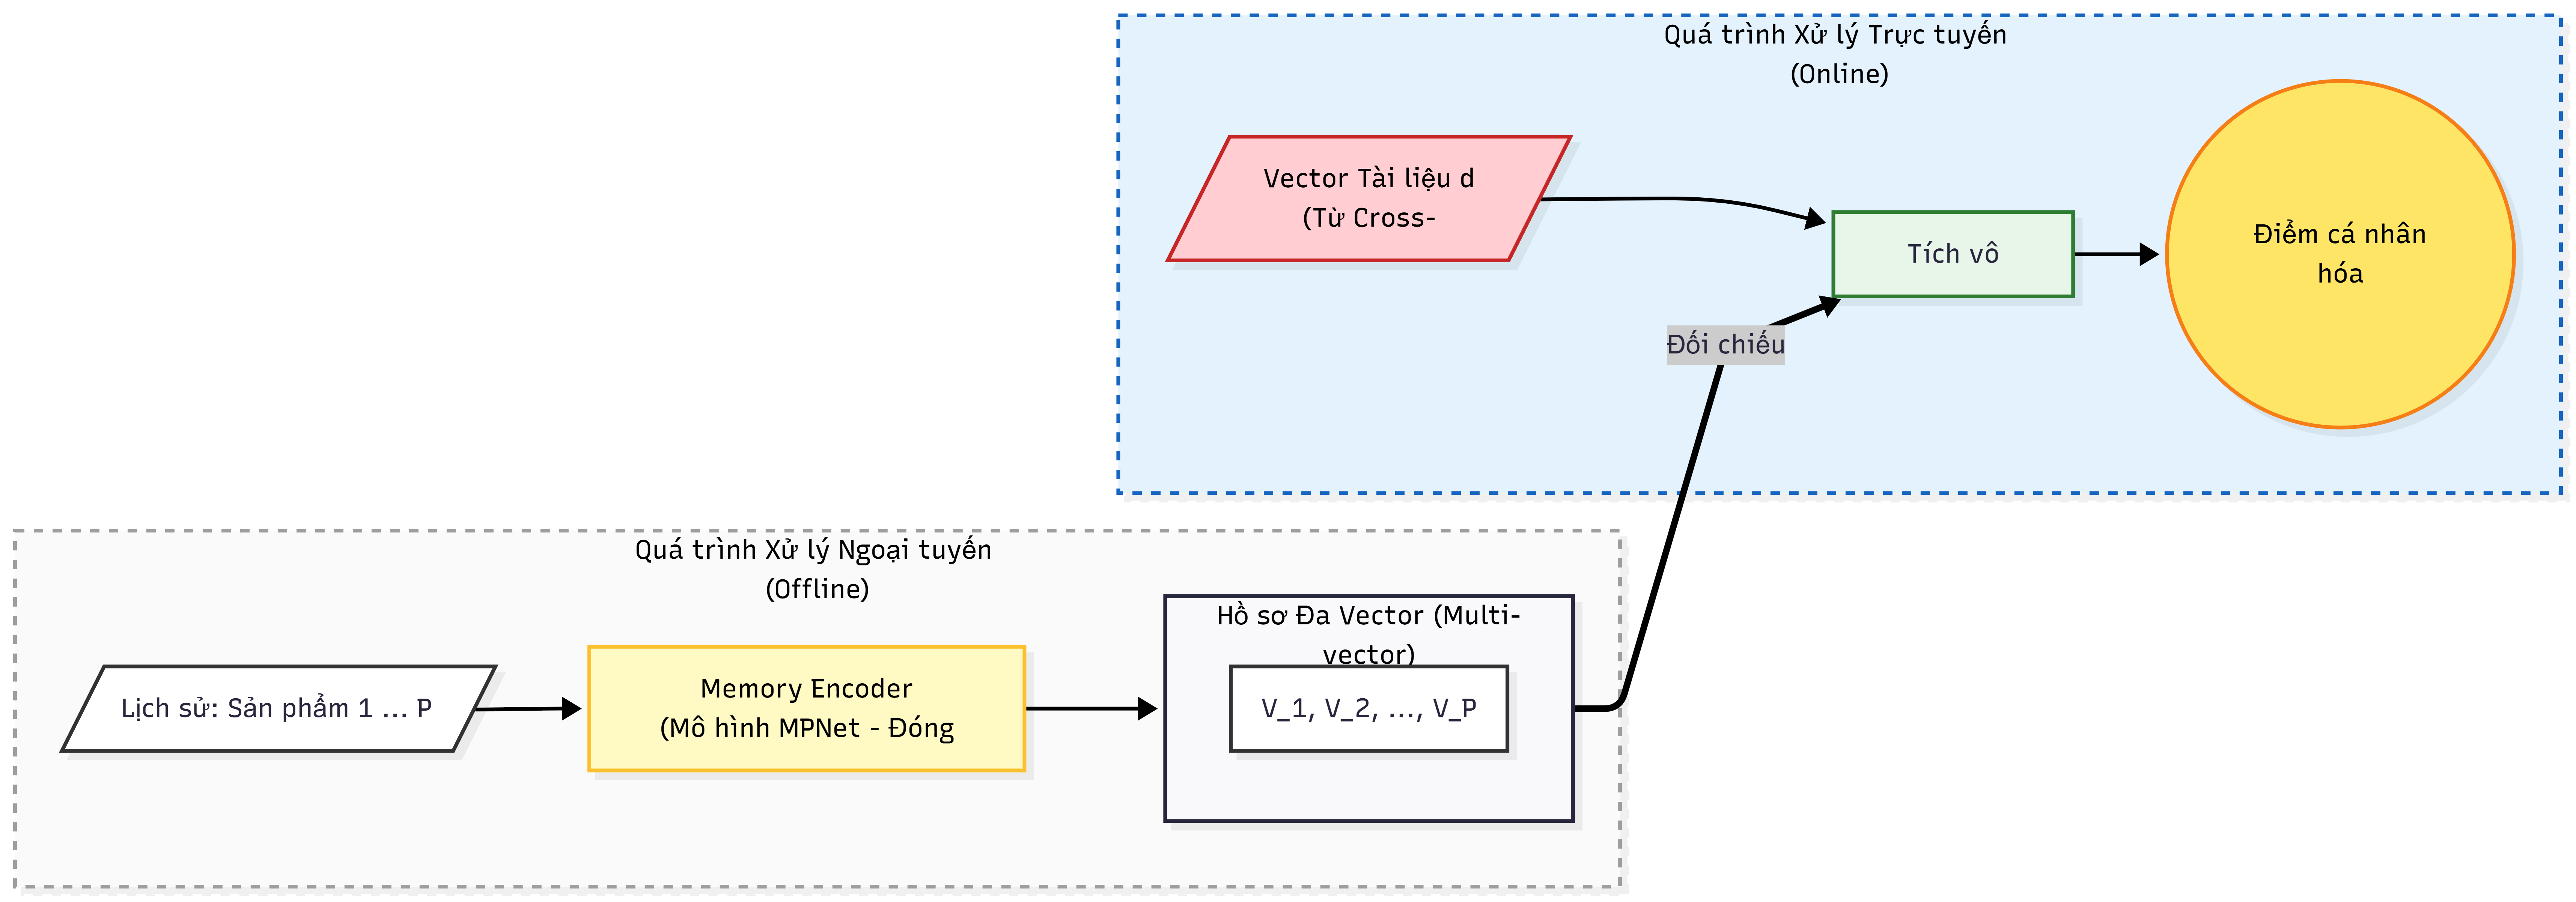
\includegraphics[width=1\textwidth]{Images/Embedding Cross-encoder-2026-04-30-153925.png} 
    \vspace{0.5cm}
    \caption{Cơ chế hoạt động của Memory Encoder phân tách thành hai luồng: Xử lý ngoại tuyến (chắt lọc hồ sơ đa vector) và Xử lý trực tuyến (đối chiếu và tính điểm cá nhân hóa).}
    \label{fig:memory_encoder}
\end{figure}

Để giải quyết bài toán này, mô-đun Memory Encoder (Bộ mã hóa ký ức) được thiết kế nhằm số hóa và quản lý hồ sơ người dùng dưới dạng một cấu trúc bộ nhớ đa vector (Multi-vector User Representation). Trong cơ chế này, lịch sử tương tác được xem như một tập hợp các tài liệu độc lập, và mỗi tài liệu cấu thành nên lịch sử đó sẽ được nạp qua một mô hình ngôn ngữ chuyên biệt nhằm tạo ra một tập hợp các vector biểu diễn ký ức ($V_i$) riêng biệt. Nhằm tối ưu hóa tài nguyên tính toán và giảm thiểu độ trễ, toàn bộ quá trình mã hóa bộ nhớ này được thực hiện ngoại tuyến (offline) với các trọng số của mô hình mã hóa được đóng băng hoàn toàn. Điểm số đánh giá mức độ cá nhân hóa ($s_d^u$) của tài liệu ứng viên được xác định dựa trên độ tương đồng vô hướng (dot product) giữa vector tài liệu mục tiêu (d) — được truyền sang từ nhánh Cross-Encoder — và từng vector ký ức trong hồ sơ người dùng. Cụ thể, hệ thống áp dụng toán tử tìm giá trị lớn nhất (max pooling) trên toàn bộ tập hợp các điểm số tương đồng vừa tính toán. Thao tác toán học này đảm bảo rằng tài liệu ứng viên chỉ cần có độ cộng hưởng mạnh mẽ với một phần sở thích cốt lõi trong quá khứ là đủ để ghi nhận điểm cá nhân hóa cao, ngăn chặn hiện tượng các tín hiệu nổi bật bị làm loãng nếu áp dụng các phép tính trung bình hóa thông thường.

Nhìn chung, Memory Encoder đóng vai trò như một bộ lọc cá nhân hóa có độ phân giải cao trong tổng thể kiến trúc xếp hạng lại. Bằng cách duy trì trực tiếp các biểu diễn vector độc lập của từng sản phẩm thay vì nén toàn bộ lịch sử thành một khối dữ liệu duy nhất, kiến trúc này bảo toàn trọn vẹn các đặc trưng chi tiết trong sở thích của người dùng. Tín hiệu cá nhân hóa độc lập và sắc bén được sinh ra từ mô-đun này không chỉ phản ánh mức độ thân thuộc của tài liệu ứng viên, mà còn cung cấp một tham chiếu định lượng thiết yếu. Đây chính là mảnh ghép dữ liệu hoàn chỉnh giúp bộ trộn ở công đoạn tiếp theo có khả năng cân đối một cách linh hoạt giữa kết quả đối sánh ngữ nghĩa và thói quen tương tác dài hạn của người dùng.


\subsection{Mixing Model}

Trong các hệ thống tìm kiếm kết hợp (hybrid search), việc trích xuất thành công hai nguồn điểm số độc lập đại diện cho độ phù hợp ngữ nghĩa và độ phù hợp cá nhân hóa mới chỉ là bước khởi đầu. Thách thức kiến trúc lớn nhất ở giai đoạn dung hợp đặc trưng nằm ở hiện tượng mất cân bằng tín hiệu, thường được nhắc đến trong lý thuyết học máy là sự sụp đổ phương thức (modality collapse) hoặc vấn đề áp đảo (dominance problem). Trên thực tế, mức độ cần thiết của thông tin cá nhân hóa biến thiên rất lớn tùy thuộc vào bản chất của từng phiên tìm kiếm: các truy vấn mang tính khám phá hoặc đa nghĩa đòi hỏi sự định hướng mạnh mẽ từ hồ sơ người dùng, trong khi các truy vấn tra cứu định danh cụ thể lại chỉ cần đối sánh từ vựng chính xác. Nếu hệ thống áp dụng một phương pháp kết hợp tuyến tính với trọng số cố định hoặc nội suy đơn giản, mô hình thường có xu hướng hội tụ về trạng thái mất cân đối, nơi nó chỉ phụ thuộc vào tín hiệu dễ học và triệt tiêu hoàn toàn vai trò của bộ nhớ lịch sử.

Nhằm khắc phục triệt để điểm yếu kiến trúc này, một mô hình trộn động (Mixing Model, ký hiệu là $g_{Mix}$) được thiết kế để điều phối toàn bộ quá trình tính toán kết quả từ các đầu vào cơ sở: câu truy vấn (q), tài liệu ứng viên (d) và hồ sơ lịch sử người dùng ($\mathcal{P}_u$). Về mặt toán học, điểm số xếp hạng cuối cùng ($s_d$) của một tài liệu được xác định thông qua phương trình nội suy kết hợp giữa tích vô hướng của các vector ngữ nghĩa và phép toán tìm cực đại trên không gian bộ nhớ:

$$s_d = w \cdot \mathbf{q}^T \mathbf{d} + (1-w) \cdot \max_{i \in \{1...P\}} \mathbf{d}^T \mathbf{V}_i$$

Trong đó, $\mathbf{q}^T \mathbf{d}$ chính là điểm phù hợp ngữ nghĩa ($s_d^q$) do Embedding Cross-Encoder trích xuất, và $\max \mathbf{d}^T \mathbf{V}_i$ là điểm cá nhân hóa ($s_d^u$) được đối chiếu từ P vector ký ức trong Memory Encoder. Trọng tâm của sự linh hoạt nằm ở việc xác định trọng số điều phối w. Thay vì gán một giá trị tĩnh, trọng số này được dự đoán liên tục thông qua một mạng nơ-ron đa tầng (MLP) kết hợp với hàm kích hoạt sigmoid nhằm giới hạn biên độ đầu ra trong khoảng [0, 1]:

$$w = \text{sigmoid}(\text{MLP}([\mathbf{q}, len(q), P, s_d^q, s_d^u]))$$

Đầu vào của mạng MLP này không chỉ dừng lại ở hai điểm số thành phần ($s_d^q$ và $s_d^u$), mà còn bao gồm một tập hợp các đặc trưng ngữ cảnh (metadata) mang tính quyết định: vector biểu diễn gốc của truy vấn ($\mathbf{q}$), độ dài của chuỗi truy vấn (len(q)), và quy mô cấu trúc của bộ nhớ người dùng (P).

Sự tích hợp của mô hình trộn động đã biến kiến trúc xếp hạng từ một cỗ máy tính toán tĩnh thành một hệ thống thích ứng ngữ cảnh mang tính dự báo. Về bản chất, thành phần này vận hành như một bộ dự báo hiệu suất (performance predictor): bằng cách phân tích hình thái của câu truy vấn và độ phong phú của dữ liệu lịch sử, nó tự động đánh giá mức độ tin cậy của nhánh đối sánh ngữ nghĩa để từ đó đưa ra quyết định cấp phát trọng số tương ứng cho nhánh cá nhân hóa. Cơ chế điều tiết tinh vi này không những giải quyết thành công bài toán áp đảo phương thức mà còn đảm bảo sự dung hòa tuyệt đối giữa ý định tìm kiếm tức thời và thói quen tiêu dùng dài hạn, cho phép hệ thống cung cấp các kết quả tìm kiếm được cá nhân hóa một cách chừng mực và tự nhiên nhất.

\subsection{Chiến thuật Huấn luyện}

\subsubsection*{Khởi tạo và thiết lập mô hình}

Quá trình huấn luyện đồng thời (end-to-end) toàn bộ kiến trúc kết hợp giữa đối sánh ngữ nghĩa và cá nhân hóa thường dẫn đến hiện tượng nhiễu loạn gradient. Sự giao thoa của các luồng tín hiệu cập nhật trọng số khác biệt có thể làm suy giảm nghiêm trọng khả năng biểu diễn ngôn ngữ cốt lõi của hệ thống. Để giải quyết rào cản này, một chiến lược huấn luyện phân tách (decoupled training) được triển khai, chia quá trình tối ưu hóa thành hai giai đoạn độc lập. Đi kèm với đó là các thiết lập khởi tạo chuyên biệt cho từng bộ mã hóa trên tập dữ liệu thương mại điện tử Amazon Review nhằm tận dụng tối đa tri thức ngôn ngữ từ các mô hình học sâu tiên tiến.

Đối với nhánh mã hóa chéo ($Enc_{CE}$), hệ thống không khởi tạo trọng số ngẫu nhiên mà kế thừa trực tiếp từ kiến trúc tiền huấn luyện \texttt{sentence-transformers/all-mpnet-base-v2}. Việc lựa chọn phiên bản này xuất phát từ hai lý do cốt lõi. Thứ nhất, về mặt nền tảng, nó vẫn kế thừa trọn vẹn kiến trúc MPNet cơ sở với khả năng tổng hợp ưu điểm của hai phương pháp học ngôn ngữ hàng đầu: cơ chế che giấu từ (Masked Language Modeling - MLM) giúp nắm bắt cấu trúc từ vựng cục bộ, và cơ chế hoán vị từ (Permuted Language Modeling - PLM) giúp hiểu được sự phụ thuộc ngữ cảnh toàn cục. Thứ hai, phiên bản \texttt{all-mpnet-base-v2} đã trải qua quá trình tối ưu hóa đặc biệt trên một bộ dữ liệu quy mô lớn gồm hơn 1 tỷ cặp câu, cung cấp một không gian vector biểu diễn tổng quát (sentence embeddings) có độ chính xác rất cao. Sau khi được khởi tạo với nền tảng trọng số mạnh mẽ này, lõi mô hình tiếp tục được tinh chỉnh (fine-tune) trực tiếp trên kho ngữ liệu của tập dữ liệu Amazon Review. Thao tác này mang ý nghĩa tiên quyết giúp mô hình làm quen với các thuật ngữ chuyên ngành, sự phân bố từ vựng đặc thù và các dạng tương tác từ vựng chéo phổ biến trong miền thương mại điện tử.

Ngược lại, đối với nhánh mã hóa ký ức ($Enc_{Mem}$), hệ thống tái sử dụng trọng số từ mô hình tiền huấn luyện \texttt{sentence-transformers/multi-qa-mpnet-base-cos-v1}. Đây là một biến thể của kiến trúc MPNet đã được tinh chỉnh chuyên sâu để tối ưu hóa cho các tác vụ hỏi đáp và truy xuất thông tin dày đặc (dense retrieval) dựa trên độ đo tương đồng cosine. Nhằm đảm bảo hệ thống có thể hoạt động trơn tru và mở rộng quy mô trên các phần cứng GPU tiêu chuẩn mà không gặp hiện tượng tràn bộ nhớ, toàn bộ hệ số trọng lượng của nhánh $Enc_{Mem}$ được đóng băng (frozen) ngay từ đầu. Chiến lược đóng băng này cho phép hệ thống thực hiện trích xuất và tính toán trước toàn bộ không gian bộ nhớ của người dùng ($\mathcal{P}_u$) một cách ngoại tuyến (offline), giúp tiết kiệm đáng kể dung lượng bộ nhớ và tài nguyên tính toán cho các công đoạn tối ưu hóa phía sau.

\subsubsection*{Giai đoạn 2 (Phase 2): Huấn luyện điều chuẩn $g_{Mix}$}

Giai đoạn huấn luyện đầu tiên được thiết kế với mục tiêu duy nhất là tối ưu hóa khả năng phân tích và trích xuất điểm số phù hợp ngữ nghĩa ($s_d^q$) của mô-đun $Enc_{CE}$ từ các cặp truy vấn và tài liệu ứng viên. Trong toàn bộ pha này, mô hình trộn cùng với điểm số cá nhân hóa hoàn toàn bị loại bỏ khỏi luồng tính toán. Sự cô lập này ép buộc nhánh mã hóa chéo phải tự mình học cách phân biệt sự liên quan ngữ nghĩa một cách khách quan nhất mà không có bất kỳ sự định hướng nào từ thông tin hồ sơ lịch sử.

Để đạt được mục tiêu tối ưu hóa, hệ thống áp dụng khung học tương phản (contrastive learning) làm nguyên lý cấu trúc dữ liệu cốt lõi. Cụ thể, đối với mỗi truy vấn q được trích xuất từ tập huấn luyện, dữ liệu đầu vào sẽ bao gồm một tài liệu tích cực đích thực (đại diện cho kết quả khớp chuẩn) đi kèm với một tập hợp gồm M tài liệu tiêu cực đóng vai trò là mồi nhử (negative samples). Tập dữ liệu ghép nối này sau khi đi qua quá trình mã hóa sẽ sinh ra một vector điểm số dự đoán liên tục, ký hiệu là $s_q$, tương ứng với một vector nhãn gốc $y_q$ mang giá trị phân phối nhị phân (trong đó duy nhất vị trí của tài liệu tích cực nhận giá trị 1, các mồi nhử còn lại nhận giá trị 0).

Quá trình cập nhật trọng số của mạng nơ-ron được dẫn dắt trực tiếp bởi hàm mất mát Softmax Cross-Entropy tiêu chuẩn. Việc áp dụng hàm loss này trên một tập hợp bao gồm cả mẫu tích cực và các mẫu tiêu cực nội lô (in-batch negatives) đã được chứng minh là phương pháp cốt lõi mang lại hiệu suất vượt trội cho các hệ thống truy xuất văn bản hiện đại \cite{22}. Về mặt toán học, hàm mất mát Softmax Cross-Entropy tiêu chuẩn \cite{22} được biểu diễn thông qua phương trình:
$$\mathcal{L}(y_q, s_q) = - \sum_{i=1}^M y_q[i] \log \text{sm}(s_q[i])$$

Trong phương trình trên, toán tử sm đại diện cho hàm phân phối xác suất softmax. Việc tối thiểu hóa hàm $\mathcal{L}$ mang một ý nghĩa hình học rõ ràng: nó tạo ra một lực đẩy ép mô hình $Enc_{CE}$ phải điều chỉnh không gian vector biểu diễn sao cho điểm số $s_d^q$ của tài liệu tích cực luôn được khuếch đại, từ đó áp đảo hoàn toàn xác suất của hàng loạt tài liệu nhiễu trong cùng một không gian đối chiếu. Kết thúc giai đoạn này, nhánh ngữ nghĩa đã đạt trạng thái sẵn sàng cao nhất để làm nền tảng cho việc dung hợp thông tin cá nhân hóa ở pha tiếp theo.

\subsubsection*{Giai đoạn 2 (Phase 2): Huấn luyện điều chuẩn $g_{Mix}$}

\textbf{Mục tiêu và Tích hợp tham số tỷ lệ:}
Bước sang giai đoạn thứ hai, trọng số của cả hai nhánh mã hóa $Enc_{CE}$ và $Enc_{Mem}$ đều được đóng băng cố định nhằm bảo toàn trọn vẹn không gian biểu diễn đã được thiết lập ở pha trước. Mục tiêu cốt lõi lúc này là tập trung huấn luyện mạng nơ-ron đa tầng của mô hình trộn $g_{Mix}$ học cách dự đoán chính xác trọng số điều phối w. Trọng số này đóng vai trò quyết định trong việc thiết lập tỷ lệ nội suy giữa điểm phù hợp ngữ nghĩa ($s_d^q$) và điểm cá nhân hóa ($s_d^u$). Điểm đáng chú ý mang tính đột phá trong kiến trúc tối ưu hóa của pha này là sự tích hợp của một tham số tỷ lệ có khả năng học (learnable scale parameter), được thiết kế lấy cảm hứng từ các mô hình mạng nơ-ron đối chiếu tiên tiến (như kiến trúc CLIP). Tham số này được khởi tạo với giá trị logarit tương đương tỷ lệ 1/0.07 (xấp xỉ 14.3) và không bị khóa cứng; ngược lại, nó được mô hình tự động tinh chỉnh linh hoạt trong suốt quá trình huấn luyện nhằm kiểm soát độ nhạy (temperature) của dải điểm số đầu ra trước khi đưa vào hàm tính toán xác suất.

\textbf{Cấu trúc dữ liệu và Mỏ neo:}
Về mặt cấu trúc dữ liệu, Giai đoạn 2 tiếp tục kế thừa nguyên vẹn tập hợp dữ liệu gồm một mẫu tích cực và M mẫu tiêu cực. Tuy nhiên, hệ thống chèn thêm một điểm mỏ neo (anchor) nhân tạo vào tập điểm số với logit mục tiêu cố định $s_0 = 0$, đi kèm với nhãn mục tiêu điều chỉnh là $y_0$ (đóng vai trò là một siêu tham số). Sự can thiệp có chủ đích này, khi được kết hợp với phép nhân vô hướng từ tham số tỷ lệ (logit scale) liên tục cập nhật, sẽ tự động khuếch đại hoặc thu hẹp khoảng cách tương đối giữa các giá trị dự đoán, từ đó biến đổi vector điểm số thô ban đầu thành $s'_q$ và vector nhãn tương ứng thành $y'_q$.

\textbf{Hàm mất mát và Ý nghĩa hiệu chuẩn:}
Để ngăn chặn tình trạng mạng MLP sinh ra các dự đoán quá tự tin (overconfident predictions) dẫn đến hiện tượng sụp đổ phương thức (modality collapse), hệ thống từ bỏ hàm Softmax tiêu chuẩn và thay thế bằng hàm Scale Calibrating Softmax Objective \cite{30}:

$$ \mathcal{L}(y'_q, s'_q) = - \sum_{i=1}^M y'_q[i] \log \frac{e^{s'_q[i]}}{\sum_j e^{s'_q[j]} + 1} + y_0 \log \left( \sum_j e^{s'_q[j]} + 1 \right) $$

Việc chèn biến neo $y_0$ vào hàm loss đóng vai trò như một cơ chế chính quy hóa (regularization) mang tính cấu trúc. Cụ thể, thành phần thứ hai của phương trình tạo ra một lực phạt nghiêm ngặt đối với các điểm số dự đoán quá lớn, trong khi thành phần thứ nhất đảm bảo các điểm số nhỏ không bị tiêu biến hoàn toàn. Dưới sự điều tiết kép của hàm loss hiệu chuẩn và tham số tỷ lệ (logit scale), trọng số w do $g_{Mix}$ sinh ra sẽ không bị cực đoan hóa về các thái cực tuyệt đối 0 hoặc 1. Thay vào đó, nó biến thiên một cách mượt mà, bám sát và phản chiếu đúng mức độ tin cậy thực tế của nhánh ngữ nghĩa, cho phép hệ thống tìm kiếm hòa trộn các tín hiệu cá nhân hóa một cách tự nhiên, chừng mực và đạt độ ổn định cao nhất.









\section{Tích hợp LLM trong Giai đoạn Hậu Truy xuất}

Trong kiến trúc tổng thể của hệ thống, Mô hình Ngôn ngữ Lớn Google Gemini được tích hợp vào giai đoạn hậu truy xuất (\textit{Post-Retrieval Stage}). Trong khi mô hình Two-Tower đóng vai trò bộ lọc thô (\textit{Coarse Filter}) giúp truy xuất nhanh các ứng viên tiềm năng dựa trên độ tương đồng vector, thì mô-đun LLM đảm nhận chức năng bộ lọc tinh và tác nhân giải thích (\textit{Explainable Agent}). Thành phần này tận dụng khả năng suy luận ngôn ngữ tự nhiên để cá nhân hóa trải nghiệm người dùng một cách sâu sắc hơn.

\subsection{Quy trình Xử lý Dữ liệu}
Quy trình tích hợp được thực hiện theo cơ chế suy luận trực tuyến (\textit{Online Inference}) thông qua bốn bước xử lý tuần tự:

\begin{enumerate}
    \item \textbf{Truy xuất Ứng viên:} \\
    Đầu vào của mô-đun là danh sách Top-$K$ sản phẩm được trả về từ mô hình Two-Tower. Tại giai đoạn này, các sản phẩm mới chỉ được định danh đơn giản bằng mã ID và điểm số tương đồng vector.
    
    \item \textbf{Làm giàu Ngữ cảnh:} \\
    Kế đến, hệ thống thực hiện các truy vấn cơ sở dữ liệu để chuyển đổi các ID vô hướng thành thông tin văn bản mang ý nghĩa ngữ nghĩa. Cụ thể:
    \begin{itemize}
        \item \textbf{Thông tin sản phẩm:} Hệ thống thu thập tiêu đề, mô tả ngắn, thông số kỹ thuật và giá tiền.
        \item \textbf{Hồ sơ người dùng:} Hệ thống truy xuất chuỗi lịch sử tương tác gần nhất, bao gồm các sản phẩm đã xem, đã mua hoặc được đánh giá cao.
    \end{itemize}
    
    \item \textbf{Kỹ thuật Prompt Engineering:} \\
    Dữ liệu sau khi làm giàu được đưa vào một khuôn mẫu cấu trúc sẵn, thiết kế theo phương pháp \textit{Zero-shot} hoặc \textit{Few-shot}. Cấu trúc này bao gồm ba thành phần chính: định nghĩa vai trò của Gemini là một chuyên gia tư vấn, cung cấp dữ liệu ngữ cảnh (lịch sử người dùng, danh sách ứng viên), và cuối cùng là nhiệm vụ yêu cầu LLM phân tích mối liên hệ sở thích để chọn lọc sản phẩm phù hợp nhất kèm theo giải thích.
    
    \item \textbf{Sinh Phản hồi:} \\
    Cuối cùng, Prompt hoàn chỉnh được gửi đến API của Gemini. Kết quả trả về là văn bản tự nhiên, sau đó được hệ thống phân tích (parse) để hiển thị lên giao diện Web Demo dưới dạng danh sách gợi ý đi kèm lời bình chi tiết.
\end{enumerate}

\subsection{Cấu trúc Prompt Minh họa}
Để LLM thực hiện tác vụ chọn lọc và giải thích mà không cần áp dụng thuật toán xếp hạng lại phức tạp, nhóm nghiên cứu sử dụng cấu trúc Prompt định hướng ngữ nghĩa như sau:

\begin{center}
\fbox{
    \begin{minipage}{0.95\textwidth}
        \setlength{\parskip}{0.5em} % Tăng khoảng cách đoạn văn trong hộp
        \textbf{System Instruction:} Bạn là một trợ lý AI chuyên nghiệp trong lĩnh vực thương mại điện tử.
        
        \textbf{User Context:} Người dùng này quan tâm đến [Danh sách lịch sử: iPhone 13, Ốp lưng MagSafe, Cáp sạc Type-C].
        
        \textbf{Candidate Items:} Dưới đây là danh sách sản phẩm tiềm năng:
        \begin{itemize}
            % Bỏ ngoặc vuông [], đưa ID ra ngoài và in đậm
            \item \textbf{ID: 101} Tai nghe AirPods Pro (Chống ồn, Apple Ecosystem)
            \item \textbf{ID: 102} Nồi cơm điện Sharp (1.8L, Nấu nhanh)
            \item \textbf{ID: 103} Sạc dự phòng Anker (20000mAh, Sạc nhanh)
        \end{itemize}
        
        \textbf{Instruction:} Dựa trên lịch sử quan tâm, hãy chọn ra các sản phẩm liên quan nhất từ danh sách ứng viên. Với mỗi sản phẩm được chọn, hãy viết một câu giải thích ngắn gọn, thuyết phục, chỉ ra mối liên hệ với sở thích cũ của họ.
    \end{minipage}
}
\end{center}

\subsection{Vai trò của LLM trong Hệ thống}
Trong cấu hình hiện tại, LLM không thay đổi thứ tự xếp hạng dựa trên điểm số mà hoạt động như một lớp hậu xử lý định tính (\textit{Qualitative Post-processing}). Cơ chế này giúp khắc phục điểm yếu hộp đen của mô hình Two-Tower bằng cách minh bạch hóa lý do gợi ý. Việc cung cấp thông tin giải thích giúp người dùng hiểu rõ sự phù hợp của sản phẩm, từ đó gia tăng niềm tin và cải thiện tỷ lệ chuyển đổi (\textit{Click-through Rate}) trên hệ thống.
\newpage
\chapter{Thực nghiệm và Đánh giá}
\label{chap:experiment}

Chương này trình bày chi tiết về quá trình thực nghiệm nhằm kiểm chứng hiệu quả của mô hình đề xuất Two-Tower Multi-modal Recommendation System. Mục tiêu của các thực nghiệm là trả lời các câu hỏi nghiên cứu sau:

\begin{enumerate}
    \item Việc kết hợp đa phương thức bao gồm ``Văn bản'', ``Hình ảnh'', ``Dữ liệu bảng'' có cải thiện hiệu năng gợi ý so với đơn phương thức hay không?
    \item Mô hình giải quyết bài toán dự đoán hành vi tiếp theo Next-Item Prediction và vấn đề Cold-start hiệu quả như thế nào?
    \item Cơ chế Hybrid Retrieval, kết hợp Query ngữ nghĩa và Personalization đóng góp ra sao vào trải nghiệm người dùng cuối?
    \item Mô hình đề xuất có khả năng triển khai trong môi trường thực tế đảm bảo yêu cầu về độ trễ thấp và tính tương tác thời gian thực hay không?
\end{enumerate}

Nội dung chương bao gồm mô tả tập dữ liệu, thiết lập môi trường thực nghiệm, định nghĩa các độ đo đánh giá, phân tích sâu các kết quả thu được và minh họa hệ thống triển khai thực tế.

\section{Mô tả tập dữ liệu}
\label{sec:data_desc}

\subsection{Tổng quan về nguồn dữ liệu}
Nghiên cứu này sử dụng tập dữ liệu \textbf{Amazon Reviews 2023}, một bộ dữ liệu quy chuẩn phổ biến trong cộng đồng nghiên cứu Hệ thống gợi ý. Cụ thể, đồ án tập trung vào phân loại hàng hóa \textit{Gift Cards}. Đây là miền dữ liệu đặc thù với tính chất sản phẩm ít biến động về cấu hình kỹ thuật nhưng phụ thuộc nhiều vào ngữ cảnh tặng quà, hình ảnh minh họa và ý định của người mua.\\

Cấu trúc dữ liệu của hệ thống được tổ chức một cách khoa học thông qua hai tập tin định dạng JSON Lines riêng biệt. Mặc dù được lưu trữ tách rời để thuận tiện cho quá trình xử lý, hai tập tin này vẫn duy trì mối liên kết logic chặt chẽ nhằm đảm bảo tính toàn vẹn của thông tin. Cụ thể, tập tin \textbf{User Reviews} đóng vai trò trung tâm trong việc lưu trữ dữ liệu người dùng, bao gồm toàn bộ lịch sử tương tác, các nội dung phản hồi đánh giá cũng như mô hình hành vi chi tiết. Song song với đó, tập tin \textbf{Item Metadata} bổ trợ bằng cách cung cấp cơ sở dữ liệu chuyên sâu về sản phẩm, bao gồm các thông tin mô tả chi tiết và dữ liệu đa phương thức, giúp định danh và làm rõ ngữ cảnh cho các đối tượng được tương tác.\\

Dưới đây là phân tích chi tiết từng trường dữ liệu được sử dụng trong quá trình huấn luyện và kiểm thử mô hình.\\

\subsubsection*{A. Chi tiết dữ liệu User Reviews}
Tập dữ liệu này đóng vai trò là nguồn ``Ground Truth'' để mô hình học sở thích của người dùng. Mỗi dòng dữ liệu đại diện cho một lần tương tác cụ thể.

\begin{table}[H]
    \centering
    \caption{Mô tả chi tiết các trường thông tin trong tập dữ liệu User Reviews}
    \label{tab:user_reviews_desc}
    \renewcommand{\arraystretch}{1.3} % Tăng khoảng cách dòng cho dễ đọc
    \begin{tabular}{|p{0.25\linewidth}|p{0.7\linewidth}|}
        \hline
        \textbf{Trường dữ liệu} & \textbf{Mô tả và Phương pháp xử lý} \\
        \hline
        \texttt{user\_id} \newline \textit{(String)} & 
        Định danh duy nhất của người dùng. Đây là khóa chính để gom nhóm lịch sử hành vi. Toàn bộ tương tác của cùng một \texttt{user\_id} được sắp xếp theo thời gian để làm đầu vào cho User Tower. \\
        \hline
        \texttt{parent\_asin} \newline \textit{(String)} & 
        Mã định danh cha của sản phẩm, đại diện cho nhóm các biến thể màu sắc và kiểu dáng. Đồ án sử dụng trường này làm khóa ngoại liên kết với Metadata nhằm giảm độ thưa dữ liệu. \\
        \hline
        \texttt{rating} \newline \textit{(Float)} & 
        Điểm đánh giá đại diện cho tín hiệu phản hồi hiện trần. Các tương tác có $\texttt{rating} \ge 4.0$ được xem là tích cực. Giá trị này cũng được dùng làm đặc trưng số học cho Tabular Encoder. \\
        \hline
        \texttt{title} \& \texttt{text} \newline \textit{(String)} & 
        \texttt{title} tóm tắt cảm xúc chính, còn \texttt{text} chứa nội dung chi tiết phản ánh lý do mua hàng. Hai trường này được nối lại thành chuỗi văn bản đầu vào cho Text Encoder. \\
        \hline
        \texttt{timestamp} \newline \textit{(Integer)} & 
        Thời gian đánh giá. Dữ liệu được sắp xếp tăng dần theo trường này để mô phỏng đúng bài toán \textit{Sequential Recommendation}, tránh rò rỉ dữ liệu tương lai. \\
        \hline
        \texttt{verified\_purchase} \newline \textit{(Boolean)} & 
        Nhãn xác thực việc mua hàng. Được mã hóa thành Embedding trong Tabular Encoder để giúp mô hình phân biệt độ tin cậy giữa tương tác thật và ảo. \\
        \hline
        \texttt{helpful\_vote} \newline \textit{(Integer)} & 
        Số lượng người khác thấy bài review hữu ích. Giá trị này được chuẩn hóa Log normalization và đưa vào mô hình như một chỉ số đo lường chất lượng tương tác. \\
        \hline
    \end{tabular}
\end{table}

\subsubsection*{B. Chi tiết dữ liệu Item Metadata}
Tập dữ liệu này cung cấp các đặc trưng nội dung để xây dựng Item Tower đa phương thức.

\begin{table}[H]
    \centering
    \caption{Mô tả chi tiết các trường thông tin trong tập dữ liệu Item Metadata}
    \label{tab:item_metadata_desc}
    \renewcommand{\arraystretch}{1.3} % Tăng khoảng cách dòng
    \begin{tabular}{|p{0.3\linewidth}|p{0.65\linewidth}|}
        \hline
        \textbf{Trường dữ liệu} & \textbf{Mô tả và Phương pháp xử lý} \\
        \hline
        \texttt{parent\_asin} \newline \textit{(String)} & 
        Khóa chính của sản phẩm. Được dùng để ánh xạ 1-nhiều với dữ liệu trong bảng User Reviews. \\
        \hline
        \texttt{title} \newline \textit{(String)} & 
        Tên đầy đủ của sản phẩm, chứa thông tin thương hiệu, mệnh giá và dịp tặng quà. Đây là đặc trưng quan trọng nhất, được mã hóa bởi BERT/MPNet để tạo vector ngữ nghĩa. \\
        \hline
        \texttt{images} \newline \textit{(List)} & 
        Danh sách ảnh sản phẩm gồm \texttt{thumb}, \texttt{large} và \texttt{hi\_res}. Ảnh chất lượng cao gồm (\texttt{hi\_res/large}) được tải về và đưa qua Vision Transformer để trích xuất đặc trưng thị giác. \\
        \hline
        \texttt{main\_category} \newline \textit{(String)} & 
        Danh mục chính (ví dụ: ``Gift Cards''). Giúp định danh miền dữ liệu. Được xử lý bằng One-hot hoặc Embedding cho Tabular Encoder. \\
        \hline
        \texttt{categories} \newline \textit{(List)} & 
        Phân cấp sản phẩm. Được xử lý để tạo embedding đại diện nhóm hàng, giúp mô hình gom cụm các sản phẩm tương đồng. \\
        \hline
        \texttt{store} \newline \textit{(String)} & 
        Thương hiệu phát hành thẻ (ví dụ: Amazon, Visa). Đây là đặc trưng định danh quan trọng, được chuyển đổi thành chỉ số Index và đưa qua lớp Embedding. \\
        \hline
        \texttt{avg\_rating} \textit{(Float)} \& \newline \texttt{rating\_number} \textit{(Int)} & 
        Điểm trung bình và tổng lượt đánh giá - các chỉ số ``Bằng chứng xã hội''. Dữ liệu này được chuẩn hóa để tránh chênh lệch thang đo khi đưa vào mạng nơ-ron. \\
        \hline
        \texttt{price} \newline \textit{(Float)} & 
        Giá bán (USD). Cung cấp thông tin phân khúc giá trị. Các giá trị thiếu được xử lý bằng phương pháp gán trung vị. \\
        \hline
        \texttt{features}, \texttt{description} \newline \& \texttt{details} & 
        Các mô tả bổ sung và thông số kỹ thuật dạng key-value. Chúng bổ sung ngữ nghĩa cho tiêu đề và được chuyển đổi thành văn bản để bổ trợ cho Text Encoder. \\
        \hline
    \end{tabular}
\end{table}

\subsubsection*{C. Mối quan hệ và Thách thức dữ liệu}
\textbf{Mối quan hệ liên kết:} Dữ liệu được liên kết thông qua trường \texttt{parent\_asin}. Quá trình tiền xử lý thực hiện phép nối Inner Join giữa Review và Metadata. Chỉ những cặp $(u, i)$ mà trong đó sản phẩm $i$ có đầy đủ thông tin, đặc biệt là ảnh và tiêu đề mới được giữ lại để huấn luyện.

\textbf{Thách thức:}Quá trình xử lý dữ liệu đối mặt với hai thách thức chính. Đầu tiên là sự \textit{đa dạng định dạng}, khi tập dữ liệu bao gồm hỗn hợp văn bản phi cấu trúc, hình ảnh, dữ liệu số và danh mục. Sự không đồng nhất này đòi hỏi kiến trúc mạng nơ-ron phải đủ phức tạp để thực hiện fusion hiệu quả các nguồn tin đa phương thức. Thách thức thứ hai đến từ \textit{nhiễu dữ liệu}, biểu hiện qua việc thiếu hụt hình ảnh, ảnh chất lượng thấp hoặc các đánh giá ngắn, thiếu ngữ nghĩa. Do đó, quy trình tiền xử lý và làm sạch dữ liệu đóng vai trò then chốt để đảm bảo chất lượng đầu vào cho mô hình.

\subsection{Phân tích chất lượng dữ liệu và Giá trị khuyết}
\label{sec:missing_data}

Để đảm bảo tính tin cậy của đầu vào mô hình, chúng tôi đã thực hiện thống kê chi tiết tỷ lệ dữ liệu khuyết trên cả hai tập dữ liệu chính: Thông tin sản phẩm và Tương tác người dùng.

\subsubsection*{A. Đối với Dữ liệu sản phẩm}
Kết quả thống kê trên tổng số \textbf{1,137} sản phẩm cho thấy sự phân hóa rõ rệt về chất lượng giữa các trường thông tin.

\begin{table}[H]
    \centering
    \caption{Thống kê tỷ lệ dữ liệu khuyết trên Item Metadata}
    \label{tab:missing_meta}
    \renewcommand{\arraystretch}{1.3} % Tăng giãn dòng giống bảng trên
    \setlength{\tabcolsep}{5pt} % Căn chỉnh khoảng cách cột
    \begin{tabular}{|p{0.25\linewidth}|c|c|p{0.35\linewidth}|}
        \hline
        \textbf{Thuộc tính} & \textbf{SL Thiếu} & \textbf{Tỷ lệ (\%)} & \textbf{Phương án xử lý} \\
        \hline
        Title & 0 & 0.00\% & Giữ nguyên. \\
        \hline
        Average Rating & 0 & 0.00\% & Sử dụng trực tiếp. \\
        \hline
        Images & 1 & 0.09\% & Loại bỏ sản phẩm hoặc dùng ảnh mặc định. \\
        \hline
        Store & 17 & 1.50\% & Gán nhãn ``Unknown''. \\
        \hline
        Features & 105 & 9.23\% & Thay thế bằng chuỗi rỗng. \\
        \hline
        Main Category & 170 & 14.95\% & Gán nhãn danh mục chung hoặc ``Gift Cards''. \\
        \hline
        Description & 262 & 23.04\% & Thay thế bằng chuỗi rỗng, tập trung vào Title. \\
        \hline
        Price & 757 & 66.58\% & Gán giá trị trung vị (Median Imputation). \\
        \hline
        Videos/Subtitle & 1137 & 100.00\% & Loại bỏ trường dữ liệu. \\
        \hline
    \end{tabular}
\end{table}

\textbf{Nhận xét và Chiến lược xử lý:}\\

Dựa trên kết quả thống kê, đồ án đề xuất chiến lược xử lý dữ liệu tập trung vào hai khía cạnh chính:\\

Đầu tiên, đối với biến \textbf{Giá}, tỷ lệ khuyết dữ liệu lên tới 66.58\% phản ánh đặc thù mệnh giá động của loại hình Gift Card. Thay vì loại bỏ trường thông tin quan trọng này, nghiên cứu áp dụng phương pháp \textit{Gán giá trị trung vị}. Phương pháp này giúp duy trì thông tin về phân khúc giá trị sản phẩm đồng thời hạn chế tác động của các giá trị ngoại lai. Tuy nhiên, để đảm bảo tính ổn định, trọng số của nhánh Tabular Encoder sẽ được điều chỉnh giảm so với các nhánh xử lý văn bản và hình ảnh.\\

Thứ hai, đối với các trường thông tin không mang lại giá trị phân tích hoặc có tỷ lệ khuyết tuyệt đối 100\% như \texttt{bought\_together}, \texttt{subtitle} và \texttt{author}, chiến lược \textit{Cắt tỉa đặc trưng} được áp dụng triệt để. Việc loại bỏ các trường này không chỉ giúp làm sạch nhiễu mà còn tối ưu hóa tài nguyên bộ nhớ và không gian lưu trữ cho quá trình huấn luyện mô hình.

\subsubsection*{B. Đối với Dữ liệu tương tác}
Trái ngược với đặc điểm phân tán của tập Metadata, dữ liệu Reviews sau quá trình sàng lọc \textit{k-core filtering} thể hiện tính toàn vẹn và độ tin cậy cao. Kết quả thống kê cho thấy tập dữ liệu bao gồm \textbf{152,410} tương tác, với tỷ lệ dữ liệu khuyết là \textbf{0\%} trên tất cả các trường thông tin trọng yếu bao gômf \texttt{user\_id}, \texttt{parent\_asin}, \texttt{rating} và \texttt{timestamp}. 

Điều này đảm bảo rằng User Tower sẽ luôn nhận được đầu vào đầy đủ và nhất quán, không cần phải thực hiện các kỹ thuật điền khuyết phức tạp cho chuỗi hành vi, giúp quá trình huấn luyện mô hình tuần tự diễn ra ổn định.
\subsection{Quy trình Tiền xử lý dữ liệu}
\label{sec:preprocessing}


Do tính chất đa phương thức và độ nhiễu cao của dữ liệu thương mại điện tử thực tế, quy trình tiền xử lý đóng vai trò then chốt trong việc đảm bảo tính hội tụ và hiệu năng của mô hình. Quy trình này được chia thành 4 giai đoạn chính: Làm sạch dữ liệu, Xử lý đặc trưng đa phương thức, Chuẩn hóa dữ liệu bảng và Xây dựng chuỗi hành vi tuần tự.

\subsubsection*{Giai đoạn 1: Làm sạch và Lọc dữ liệu}
Dữ liệu thô thu thập từ Amazon thường chứa nhiều giá trị bị khuyết và các điểm dữ liệu nhiễu. Quy trình tiền xử lý dữ liệu được tiến hành qua hai giai đoạn trọng tâm nhằm chuẩn hóa đầu vào cho mô hình, các bước xử lý bao gồm:\\

Giai đoạn thứ nhất tập trung vào \textbf{xử lý giá trị khuyết} với các chiến lược riêng biệt cho từng loại dữ liệu. Cụ thể, các mẫu thiếu trường định danh cốt lõi như \texttt{title} sẽ bị loại bỏ hoàn toàn để đảm bảo tính nhất quán. Đối với dữ liệu số học như \texttt{price}, phương pháp gán giá trị trung vị được ưu tiên áp dụng thay vì giá trị trung bình, giúp giảm thiểu tác động lệch chuẩn gây ra bởi các giá trị ngoại lai. Trong khi đó, các giá trị rỗng tại các trường văn bản bổ trợ như \texttt{features} hay \texttt{description} được xử lý bằng cách điền thế chuỗi ký tự trống ``'' để đảm bảo tính hợp lệ kỹ thuật cho bộ mã hóa.\\

Giai đoạn thứ hai là \textbf{sàng lọc tương tác}, áp dụng kỹ thuật \textit{k-core filtering} với ngưỡng $k=3$ nhằm tối ưu hóa dữ liệu cho bài toán \textit{Sequential Recommendation}. Về phía người dùng, hệ thống loại bỏ các tài khoản có dưới 3 tương tác, Cold-start Users, do nhóm này không cung cấp đủ độ dài chuỗi lịch sử cần thiết để mô hình Transformer học được các mẫu hành vi phụ thuộc. Song song với đó, các sản phẩm có tần suất xuất hiện quá thấp, dưới 2 lần, cũng được lược bỏ để đảm bảo không gian biểu diễn được học từ dữ liệu đủ dày đặc.

\subsubsection*{Giai đoạn 2: Xử lý đặc trưng phi cấu trúc}
Đây là bước chuẩn bị đầu vào cho hai nhánh mạng nơ-ron chính: Text Encoder và Image Encoder.

\textbf{1. Xử lý dữ liệu văn bản:} \\
Do thông tin ngữ nghĩa của sản phẩm nằm rải rác ở nhiều trường khác nhau, chúng tôi thực hiện chiến lược nối chuỗi:
\begin{equation}
    \text{Text}_{input} = [\text{Title}] \oplus [\text{Description}] \oplus [\text{Features}] \oplus [\text{Details}]
\end{equation}
Trong đó $\oplus$ là phép nối chuỗi kèm theo ký tự phân cách đặc biệt. Chuỗi văn bản tổng hợp này sau đó được đưa qua bộ phân tách từ của mô hình \texttt{all-mpnet-base-v2}. Quá trình Tokenization tuân thủ các quy tắc:
\begin{itemize}
    \item \textbf{Padding:} Các chuỗi ngắn hơn độ dài tối đasẽ được thêm token \texttt{[PAD]} để đảm bảo kích thước batch đồng nhất.
    \item \textbf{Truncation:} Các chuỗi quá dài sẽ bị cắt bớt để phù hợp với giới hạn đầu vào của BERT, thường là 512 tokens, ưu tiên giữ lại phần đầu của văn bản vì chứa thông tin quan trọng nhất.
\end{itemize}

\textbf{2. Xử lý dữ liệu hình ảnh:} \\
Dữ liệu ảnh được tải về từ các đường dẫn URL trong Metadata. Quy trình xử lý ảnh tuân theo chuẩn đầu vào của mô hình Vision Transformer:
\begin{itemize}
    \item \textbf{Tải và Lọc lỗi:} Sử dụng Multi-threading để tải ảnh. Các ảnh bị lỗi định dạng hoặc không thể tải sẽ bị loại bỏ hoặc thay thế bằng ảnh placeholder màu đen.
    \item \textbf{Resize \& Center Crop:} Ảnh được thay đổi kích thước về độ phân giải $224 \times 224$ pixels.
    \item \textbf{Chuẩn hóa:} Các giá trị pixel trong khoảng $[0, 255]$ được chuyển về khoảng $[0, 1]$ và sau đó được chuẩn hóa theo phân bố của tập dữ liệu ImageNet:
    \begin{equation}
        x_{norm} = \frac{x - \mu_{ImageNet}}{\sigma_{ImageNet}}
    \end{equation}
    Với $\mu = [0.485, 0.456, 0.406]$ và $\sigma = [0.229, 0.224, 0.225]$. Bước này giúp mô hình ViT pretrained hoạt động hiệu quả nhất.
\end{itemize}

\subsubsection*{Giai đoạn 3: Xử lý dữ liệu bảng}
Dữ liệu có cấu trúc bao gồm các biến phân loại và biến số được xử lý riêng biệt.\\

\textbf{1. Biến phân loại (\texttt{main\_category}, \texttt{store}):}
    Được chuyển đổi sang dạng số nguyên (Integer Mapping) thông qua kỹ thuật Label Encoding. Một từ điển (Vocabulary) được xây dựng để ánh xạ mỗi giá trị duy nhất (ví dụ: ``Starbucks'') sang một chỉ số ID (ví dụ: 124). Các giá trị mới xuất hiện trong tập Test sẽ được gán về token đặc biệt \texttt{<UNK>}.\\
    
\textbf{2. Biến danh sách phân loại (\texttt{categories}):}
    Một sản phẩm có thể thuộc nhiều danh mục con (ví dụ: [Gift Cards, Birthday, For Her]). Chúng tôi sử dụng phương pháp \textit{Multi-hot Encoding} kết hợp với \textit{Embedding Pooling}. Cụ thể, các ID của danh mục sẽ được tra cứu trong bảng Embedding, sau đó lấy trung bình (Average Pooling) để tạo ra một vector đại diện duy nhất cho trường này.\\
    
\textbf{3. Biến số (\texttt{rating}, \texttt{vote}, \texttt{price}):}
    Để giúp mạng nơ-ron hội tụ nhanh hơn, các biến số được chuẩn hóa bằng \textit{Standard Scaler} (Z-score normalization):
    \begin{equation}
        z = \frac{x - \mu}{\sigma}
    \end{equation}
    Riêng đối với biến \texttt{helpful\_vote}, do phân bố lệch trái nặng (phần lớn là 0 hoặc số nhỏ), chúng tôi áp dụng biến đổi Logarit trước khi chuẩn hóa: $x' = \log(1 + x)$.

\subsubsection*{Giai đoạn 4: Xây dựng chuỗi tương tác}
Đây là bước quan trọng nhất để huấn luyện User Tower. Dữ liệu tương tác được gom nhóm theo \texttt{user\_id} và sắp xếp tăng dần theo \texttt{timestamp}.

Với mỗi người dùng $u$, ta có chuỗi hành vi $S_u = \{i_1, i_2, ..., i_T\}$. Quá trình tạo mẫu huấn luyện (Training Samples) được thực hiện theo cơ chế \textit{Sliding Window}:
\begin{itemize}
    \item Tại mỗi bước thời gian $t$ ($1 < t \le T$), mô hình sử dụng chuỗi lịch sử $H_t = \{i_1, ..., i_{t-1}\}$ để dự đoán item mục tiêu $i_t$.
    \item \textbf{Padding:} Nếu độ dài chuỗi lịch sử nhỏ hơn độ dài tối đa quy định ($L=40$), chúng tôi thêm các token \texttt{[PAD]} vào bên trái chuỗi.
    \item \textbf{Masking:} Một ma trận mặt nạ được tạo ra để báo cho lớp Self-Attention trong Transformer biết cần bỏ qua các vị trí là \texttt{[PAD]}, đảm bảo tính toán chỉ tập trung vào các tương tác thực tế.
\end{itemize}
Thống kê chi tiết được trình bày trong Bảng \ref{tab:dataset_stats}.

\begin{table}[H]
    \centering
    \caption{Thống kê tập dữ liệu Amazon Gift Cards sau khi tiền xử lý}
    \label{tab:dataset_stats}
    \renewcommand{\arraystretch}{1.3} % Tăng khoảng cách dòng
    \setlength{\tabcolsep}{5pt} % Căn chỉnh khoảng cách cột
    \begin{tabular}{|p{0.35\linewidth}|c|p{0.4\linewidth}|}
        \hline
        \textbf{Thông số} & \textbf{Số lượng} & \textbf{Mô tả} \\
        \hline
        Tổng số người dùng  & 73,929 & Số lượng người dùng duy nhất. \\
        \hline
        Tổng số sản phẩm & 1,137 & Số lượng thẻ quà tặng khác nhau. \\
        \hline
        Tổng số tương tác & 78,095 & Tổng số lượt review/rating hợp lệ. \\
        \hline
        Độ dài chuỗi trung bình & $\sim 1.06$ & Số lượng tương tác trung bình trên một người dùng. \\
        \hline
    \end{tabular}
\end{table}
Kết quả của quá trình tiền xử lý là các Tensor định dạng PyTorch sẵn sàng được đưa vào GPU để huấn luyện.

\subsection{Phân tích độ thưa dữ liệu}
\label{sec:sparsity_analysis}

\subsubsection*{A. Cơ sở lý thuyết và Định nghĩa}
Trong các hệ thống gợi ý, dữ liệu thường được biểu diễn dưới dạng một ma trận tương tác User-Item $R$ có kích thước $|U| \times |I|$, trong đó $|U|$ là tổng số người dùng và $|I|$ là tổng số sản phẩm. Mỗi phần tử $r_{ui}$ trong ma trận biểu thị tương tác của người dùng $u$ lên sản phẩm $i$.

Độ thưa phản ánh tỷ lệ các phần tử rỗng trong ma trận này. Một ma trận có độ thưa quá cao đồng nghĩa với việc thông tin hành vi người dùng cực kỳ hạn chế, gây khó khăn cho việc tìm kiếm các mẫu tương đồng. Độ thưa được định nghĩa bởi công thức \cite{31}:

\begin{equation}
    \text{Sparsity} = 1 - \text{Density} = 1 - \frac{\text{Total Interactions}}{|U| \times |I|}
\end{equation}

\subsubsection*{B. Tính toán thực nghiệm trên tập dữ liệu Amazon}
Dựa trên các thống kê đã trình bày ở Bảng \ref{tab:dataset_stats}, chúng tôi tiến hành tính toán độ thưa cụ thể cho tập dữ liệu huấn luyện:

\begin{itemize}
    \item Tổng số người dùng ($|U|$): $73,929$
    \item Tổng số sản phẩm ($|I|$): $1,137$
    \item Tổng số tương tác quan sát được ($N$): $78,095$
\end{itemize}

Kích thước không gian mẫu là:
$$ |U| \times |I| = 73,929 \times 1,137 \approx 84,057,273 $$

Mật độ dữ liệu thực tế:
$$ \text{Density} = \frac{78,095}{84,057,273} \approx 0.000929 \ ( 0.09\%) $$

Từ đó, độ thưa của tập dữ liệu là:
$$ \text{Sparsity} = 1 - 0.000929 \approx 0.999071 \ (\mathbf{99.91\%}) $$

\subsubsection*{C. Đánh giá và Tác động đến mô hình}
Kết quả tính toán $99.82\%$ cho thấy tập dữ liệu Amazon Gift Cards thuộc nhóm ``Extreme Sparsity''. Để so sánh, các tập dữ liệu chuẩn như MovieLens-1M thường có độ thưa khoảng $95-96\%$. Việc độ thưa tiệm cận $100\%$ đặt ra hai thách thức nghiêm trọng:\\


 Thứ nhất, \textbf{sự thất bại của Collaborative Filtering thuần túy:} Các thuật toán CF truyền thống như Matrix Factorization dựa vào việc tìm kiếm người dùng có hành vi tương đồng hoặc sản phẩm tương đồng thông qua sự chồng lấp các tương tác. Với mật độ $0.09\%$, xác suất để hai người dùng bất kỳ cùng đánh giá một sản phẩm là cực thấp, dẫn đến việc mô hình không thể tính toán độ tương đồng tin cậy.\\
    
Thứ hai, \textbf{vấn đề Cold-start:} Phần lớn người dùng trong tập dữ liệu chỉ có số lượng tương tác tối thiểu khoảng 2-3 tương tác. Mô hình không có đủ lịch sử hành vi để học được vector đại diện User Embedding chính xác nếu chỉ dựa vào ID.


\subsubsection*{D. Giải pháp tiếp cận: Content-based Multi-modal Learning}
Chính vì thách thức về độ thưa nêu trên, đồ án này bắt buộc phải chuyển hướng từ việc chỉ khai thác dữ liệu tương tác sang khai thác dữ liệu nội dung.

Cụ thể, kiến trúc Two-Tower được thiết kế để tận dụng các đặc trưng giàu ngữ nghĩa luôn có sẵn, bất kể người dùng đã tương tác hay chưa:
\begin{itemize}
    \item \textbf{Text Encoder (BERT):} Giúp mô hình hiểu rằng ``Visa Gift Card'' và ``Mastercard Gift Card'' là tương đồng về mặt ngữ nghĩa, ngay cả khi chưa có người dùng nào mua cả hai.
    \item \textbf{Image Encoder (ViT):} Giúp liên kết các sản phẩm có hình thức trình bày giống nhau (ví dụ: cùng chủ đề Giáng sinh, Sinh nhật) thông qua đặc trưng thị giác.
    \item \textbf{Tabular Encoder (MLP):} Xử lý các dữ liệu cấu trúc như \textit{Giá bán, Điểm đánh giá, Thương hiệu}. Nhánh này giúp mô hình học được các ngưỡng lọc quan trọng (ví dụ: người dùng chỉ thích mua thẻ mệnh giá thấp $<\$50$) để thu hẹp không gian tìm kiếm hiệu quả.
\end{itemize}

Nhờ cơ chế Fusion Gate kết hợp các thông tin này, mô hình có thể lấp đầy các khoảng trống trong ma trận thưa bằng các suy luận dựa trên nội dung, từ đó cải thiện đáng kể độ chính xác gợi ý như Recall hay NDCG sẽ được trình bày trong phần Kết quả thực nghiệm.

% [PLACEHOLDER CHO ẢNH]
% Bạn hãy thêm ảnh Histogram phân bố độ dài chuỗi hành vi của User vào đây
%\begin{figure}[H]
%%%    \centering
%%%    
\includegraphics[width=0.8\textwidth]{imagedothua.png} 
%%%    \caption{Phân bố độ dài chuỗi hành vi người dùng}
%%%    \label{fig:seq_dist}
%%%\end{figure}

\section{Thiết lập thực nghiệm}

\subsection{Môi trường phần cứng và phần mềm}
\subsubsection*{Cơ sở hạ tầng phần cứng}
Các thực nghiệm được triển khai trên nền tảng đám mây \textbf{Kaggle Kernels}, tận dụng sức mạnh tính toán hiệu năng cao của Google Cloud Platform (GCP). Việc sử dụng môi trường đám mây giúp giảm thiểu các sai số do sự khác biệt về phần cứng cá nhân và đảm bảo mô hình được huấn luyện trong điều kiện tối ưu.

Chi tiết cấu hình phần cứng như sau:

\begin{itemize}
    \item \textbf{Bộ xử lý đồ họa (GPU) :}
\begin{itemize}
        \item \textit{Loại thiết bị:} \textbf{NVIDIA Tesla P100-PCIE}.
        \item \textit{Kiến trúc:} Pascal.
        \item \textit{Bộ nhớ đồ họa (VRAM):} $16$ GB \textbf{HBM2}.
        \item \textit{Lý do lựa chọn:} Mặc dù là kiến trúc Pascal, Tesla P100 sở hữu băng thông bộ nhớ vượt trội ($\sim 732$ GB/s), cao hơn đáng kể so với các dòng GPU sử dụng bộ nhớ GDDR6 thông thường (như Tesla T4). Đặc điểm này cực kỳ tối ưu cho mô hình Two-Tower, nơi tác vụ Embedding Lookup cho hàng nghìn User/Item tiêu tốn tài nguyên băng thông rất lớn.
    \end{itemize}
    
    \item \textbf{Bộ xử lý trung tâm (CPU):}
    \begin{itemize}
        \item \textit{Cấu hình:} Intel(R) Xeon(R) CPU @ 2.20GHz (4 cores, 8 threads).
        \item \textit{Vai trò:} Chịu trách nhiệm cho các tác vụ tiền xử lý dữ liệu, tải ảnh đa luồng  và đưa dữ liệu vào hàng đợi trước khi đẩy sang GPU.
    \end{itemize}
    
    \item \textbf{Bộ nhớ trong (RAM):}
    \begin{itemize}
        \item \textit{Dung lượng:} $32$ GB System RAM.
        \item \textit{Vai trò:} Đảm bảo toàn bộ Meta-data và các vector đặc trưng sau khi trích xuất có thể được lưu trữ trên bộ nhớ đệm, tránh hiện tượng nghẽn cổ chai do đọc/ghi đĩa cứng liên tục.
    \end{itemize}
\end{itemize}

\subsubsection*{Hệ sinh thái phần mềm và Thư viện}
Mô hình được phát triển dựa trên ngôn ngữ lập trình \textbf{Python} phiên bản 3.10, ngôn ngữ tiêu chuẩn trong cộng đồng Trí tuệ nhân tạo hiện nay. Chúng tôi sử dụng các framework mã nguồn mở tiên tiến nhất để xây dựng kiến trúc mạng nơ-ron sâu.

Các thư viện chính bao gồm:

\begin{itemize}
    \item \textbf{PyTorch (v2.0+):} 
    Framework nền tảng cho Deep Learning. PyTorch được lựa chọn nhờ cơ chế đồ thị tính toán động, giúp linh hoạt trong việc xây dựng các kiến trúc phức tạp như Fusion Gate và tùy chỉnh hàm mất mát Contrastive Loss.
    
    \item \textbf{Hugging Face Transformers:} 
    Thư viện chuẩn mực cho các mô hình NLP. Chúng tôi sử dụng thư viện này để tải trọng số tiền huấn luyện của mô hình \texttt{all-mpnet-base-v2} và thực hiện quy trình Tokenization văn bản.
    
    \item \textbf{TIMM (PyTorch Image Models):} 
    Thư viện chuyên dụng cho các mô hình thị giác máy tính hiện đại. TIMM cung cấp kiến trúc \texttt{vit\_base\_patch16\_224} cùng các trọng số đã được huấn luyện trên ImageNet, giúp trích xuất đặc trưng ảnh chính xác mà không cần huấn luyện lại từ đầu.
    
    \item \textbf{Scikit-learn \& Pandas:} 
    Sử dụng cho các tác vụ xử lý dữ liệu bảng, phân chia tập dữ liệu, chuẩn hóa dữ liệu và tính toán các độ đo đánh giá cơ bản.
    
    \item \textbf{Các thư viện hỗ trợ khác:} 
    \begin{itemize}
        \item \texttt{tqdm}: Để theo dõi tiến độ huấn luyện trực quan.
        \item \texttt{matplotlib/seaborn}: Để trực quan hóa dữ liệu và biểu đồ Loss.
        \item \texttt{PIL (Pillow)}: Để xử lý và biến đổi dữ liệu ảnh thô.
    \end{itemize}
\end{itemize}


\subsection{Cấu hình Siêu tham số}
Quá trình huấn luyện được chia làm 2 giai đoạn: Huấn luyện Item Tower trước để tạo vector đặc trưng sản phẩm, sau đó dùng các vector này đóng băng hoặc tinh chỉnh nhẹ để huấn luyện User Tower.

\subsubsection*{Cấu hình Item Tower}
Item Tower chịu trách nhiệm mã hóa thông tin đa phương thức của sản phẩm. Các tham số chi tiết được liệt kê trong Bảng \ref{tab:item_params}.

\begin{table}[H]
    \centering
    \caption{Cấu hình siêu tham số cho Item Tower}
    \label{tab:item_params}
    \vspace{0.2cm}
    \begin{tabular}{l l p{6cm}}
        \toprule
        \textbf{Tham số} & \textbf{Giá trị} & \textbf{Giải thích} \\
        \midrule
        Text Encoder & \texttt{all-mpnet-base-v2} & Mô hình Sentence-BERT tối ưu cho Semantic Search \\
        Image Encoder & \texttt{vit\_base\_patch16\_224} & Vision Transformer pretrained trên ImageNet \\
        Batch Size & 128 & Kích thước lô dữ liệu \\
        Learning Rate & $2 \times 10^{-5}$ & Tốc độ học thấp để fine-tune \\
        Epochs & 70 & Số vòng lặp huấn luyện \\
        Temperature ($\tau$) & 0.07 & Tham số nhiệt độ cho Contrastive Loss \\
        Latent Dimension & 256 & Kích thước vector nhúng cuối cùng \\
        \bottomrule
    \end{tabular}
\end{table}

\subsubsection*{Cấu hình User Tower}
User Tower sử dụng kiến trúc Transformer Encoder để học sự phụ thuộc tuần tự trong lịch sử hành vi người dùng.

\begin{table}[H]
    \centering
    \caption{Cấu hình siêu tham số cho User Tower}
    \label{tab:user_params}
    \vspace{0.2cm}
    \begin{tabular}{l l p{6cm}}
        \toprule
        \textbf{Tham số} & \textbf{Giá trị} & \textbf{Giải thích} \\
        \midrule
        Architecture & Transformer Encoder & Sử dụng Self-Attention \\
        Num Layers & 2 & Số lớp Transformer \\
        Num Heads & 4 & Số đầu Attention \\
        Max Seq Length & 40 & Độ dài chuỗi lịch sử tối đa \\
        LR (Base) & $1 \times 10^{-4}$ & Cho các lớp khởi tạo mới (Fusion, Projection) \\
        LR (Pretrained) & $1 \times 10^{-6}$ & Cho các lớp BERT/Embedding (Differential Learning Rates) \\
        Batch Size & 64 & Giảm batch size do mô hình phức tạp \\
        \bottomrule
    \end{tabular}
\end{table}
\section{Đầu vào và đầu ra}
\label{sec:inputoutput}
\subsection{Xây dựng Item Tower}

Item Tower đóng vai trò trích xuất đặc trưng từ dữ liệu đa phương thức của sản phẩm để tạo ra một vector đại diện thống nhất. Để đảm bảo tính nhất quán trong tính toán, chúng tôi quy ước các ký hiệu kích thước như sau:
\begin{itemize}
    \item $B$: Kích thước Batch Size, ví dụ $B=128$.
    \item $D_{orig}$: Số chiều gốc của các mô hình Pre-trained, với MPNet và ViT-Base là $768$.
    \item $D$: Số chiều không gian tiềm ẩn đích, thiết lập $D=256$.
\end{itemize}

\subsubsection*{Text Encoder}
Hệ thống sử dụng mô hình ngôn ngữ \textbf{all-mpnet-base-v2} để chuyển đổi thông tin văn bản gồm Tiêu đề và Mô tả thành vector ngữ nghĩa.

\begin{table}[H]
    \centering
    \caption{Đặc tả luồng dữ liệu và kích thước trong Text Encoder}
    \vspace{0.2cm}
    \begin{tabular}{|l|l|p{6cm}|}
    \hline
    \textbf{Tầng xử lý} & \textbf{Kích thước} & \textbf{Giải thích chi tiết} \\ \hline
    \textbf{1. Input Raw} & List[String] kích thước $B$ & Danh sách các chuỗi văn bản thô đầu vào. \\ \hline
    \textbf{2. Tokenization} & $(B, L_{max})$ & Văn bản được phân tách thành các Token IDs. $L_{max}=512$ là độ dài chuỗi tối đa. Các chuỗi ngắn hơn được padding giá trị 0. \\ \hline
    \textbf{3. Transformer Backbone} & $(B, L_{max}, 768)$ & Đầu ra từ lớp ẩn cuối cùng của MPNet. Mỗi token trong chuỗi được biểu diễn bởi một vector 768 chiều. \\ \hline
    \textbf{4. Mean Pooling} & $(B, 768)$ & Thực hiện phép trung bình cộng dọc theo trục chiều dài chuỗi ($L_{max}$), loại bỏ các token đệm để thu được vector đại diện cho toàn bộ câu. \\ \hline
    \textbf{5. Projection Head} & $\mathbf{(B, 256)}$ & Lớp tuyến tính nén vector từ 768 xuống 256 chiều, đóng vai trò là đầu ra của nhánh văn bản ($v_{text}$). \\ \hline
    \end{tabular}
\end{table}

\subsubsection*{Image Encoder}
Sử dụng kiến trúc \textbf{Vision Transformer ViT-Base-Patch16-224} để trích xuất đặc trưng thị giác từ ảnh sản phẩm.

\begin{table}[H]
    \centering
    \caption{Đặc tả luồng dữ liệu và kích thước trong Image Encoder}
    \vspace{0.2cm}
    \begin{tabular}{|l|l|p{6cm}|}
    \hline
    \textbf{Tầng xử lý} & \textbf{Kích thước} & \textbf{Giải thích chi tiết} \\ \hline
    \textbf{1. Input Image} & $(B, 3, 224, 224)$ & Ảnh RGB gốc được resize về kích thước $224 \times 224$ pixels và chuẩn hóa theo phân phối ImageNet. \\ \hline
    \textbf{2. Patch Embedding} & $(B, 197, 768)$ & Ảnh được chia thành lưới $14 \times 14 = 196$ patches. Cộng thêm 1 token đặc biệt \texttt{[CLS]} ở đầu chuỗi để học đặc trưng toàn cục. \\ \hline
    \textbf{3. Transformer Encoder} & $(B, 197, 768)$ & Các patch đi qua 12 lớp Self-Attention của ViT. Kích thước không đổi. \\ \hline
    \textbf{4. Feature Extraction} & $(B, 768)$ & Chỉ lấy vector tại vị trí đầu tiên (index 0, ứng với token \texttt{[CLS]}), đại diện cho nội dung toàn bức ảnh. \\ \hline
    \textbf{5. Projection Head} & $\mathbf{(B, 256)}$ & Chiếu vector đặc trưng về không gian chung 256 chiều ($v_{img}$). \\ \hline
    \end{tabular}
\end{table}

\subsubsection*{Tabular Encoder}
Xử lý các thông tin định lượng như Giá và Rating, và các thông tin định danh như Danh mục và Thương hiệu.

\begin{table}[H]
    \centering
    \caption{Đặc tả luồng dữ liệu trong Tabular Encoder}
    \vspace{0.2cm}
    \begin{tabular}{|l|l|p{6cm}|}
    \hline
    \textbf{Tầng xử lý} & \textbf{Kích thước (Shape)} & \textbf{Giải thích chi tiết} \\ \hline
    \textbf{1. Input Features} & $(B, N_{feat})$ & Vector chứa giá trị số đã chuẩn hóa Z-score và index của biến phân loại. \\ \hline
    \textbf{2. Embedding Lookup} & $(B, N_{cat} \times D_{emb})$ & Các biến phân loại được chuyển thành vector nhúng và nối \lại với nhau. \\ \hline
    \textbf{3. Concatenation} & $(B, D_{total})$ & Ghép nối vector biến số thực và vector biến phân loại thành một vector dài. \\ \hline
    \textbf{4. MLP Block} & $\mathbf{(B, 256)}$ & Mạng nơ-ron đa tầng (Linear $\to$ ReLU $\to$ Linear) biến đổi dữ liệu hỗn hợp thành vector đặc trưng bảng ($v_{tab}$). \\ \hline
    \end{tabular}
\end{table}

\subsubsection*{Cơ chế Fusion}
Mô-đun \textbf{Fusion Gate} chịu trách nhiệm tổng hợp ba nguồn thông tin trên thành một vector duy nhất. Quá trình này diễn ra như sau:

\begin{enumerate}
    \item \textbf{Xếp chồng:} Ba vector đầu ra từ các encoder được xếp chồng lên nhau tạo thành tensor đầu vào $V_{in}$:
    $$ V_{in} = [v_{text}, v_{img}, v_{tab}] \in \mathbb{R}^{B \times 3 \times 256} $$
    
    \item \textbf{Tính trọng số chú ý:} Một mạng nơ-ron nhỏ (Linear layer) học cách đánh giá độ quan trọng của từng modal dựa trên ngữ cảnh:
    $$ W_{raw} = V_{in} \times W_{learnable} \in \mathbb{R}^{B \times 3 \times 1} $$
    $$ \alpha = \text{Softmax}(W_{raw}) \in \mathbb{R}^{B \times 3 \times 1} $$
    Trong đó $\sum_{k=1}^3 \alpha_{i,k} = 1$ với mọi mẫu dữ liệu $i$.
    
    \item \textbf{Tổng hợp có trọng số:} Vector sản phẩm cuối cùng là tổng của các vector thành phần nhân với trọng số tương ứng:
    $$ v_{item} = \sum_{k \in \{text, img, tab\}} \alpha_k \cdot v_k $$
    \textbf{Output:} Tensor $v_{item}$ có kích thước $\mathbf{(B, 256)}$.
\end{enumerate}

Kết quả cuối cùng là mỗi sản phẩm trong hệ thống được đại diện bởi một vector 256 chiều duy nhất, chứa đựng tinh hoa thông tin được chắt lọc từ cả hình ảnh, văn bản và dữ liệu bảng.
\subsection{Xây dựng User Tower}
\label{sec:user_tower}

Khác với các mô hình tuần tự truyền thống như SASRec chỉ dựa vào định danh sản phẩm Item ID, User Tower trong đồ án này được thiết kế theo kiến trúc \textit{Mạng Tuần tự Đa phương thức}. Tại mỗi bước thời gian $t$ trong lịch sử hành vi, mô hình không chỉ nhìn thấy sản phẩm mà còn đọc được nội dung bài đánh giá và hiểu được mức độ hài lòng của người dùng tại thời điểm đó.

Quy ước kích thước:
\begin{itemize}
    \item $B$: Kích thước Batch Size.
    \item $S$: Độ dài chuỗi lịch sử tối đa, thiết lập $S=50$.
    \item $D$: Số chiều không gian tiềm ẩn đích, $D=256$.
\end{itemize}

\subsubsection*{Đầu vào đa nguồn}
User Tower tiếp nhận 4 luồng dữ liệu song song đại diện cho chuỗi hành vi của người dùng:

\begin{table}[H]
    \centering
    \caption{Đặc tả các luồng dữ liệu đầu vào cho User Tower}
    \vspace{0.2cm}
    \begin{tabular}{|l|l|p{8cm}|}
    \hline
    \textbf{Luồng dữ liệu} & \textbf{Kích thước} & \textbf{Mô tả chi tiết} \\ \hline
    \textbf{1. Item Indices} & $(B, S)$ & Chuỗi ID các sản phẩm đã tương tác. Các chuỗi ngắn hơn $S$ được đệm bằng giá trị $0$. \\ \hline
    \textbf{2. Review Texts} & List[$B \times S$] & Nội dung văn bản mà user đã viết cho từng sản phẩm, ví dụ: ``Thẻ này rất tiện'', ``Giao hàng chậm''. \\ \hline
    \textbf{3. Context Feats} & $(B, S, 3)$ & Các đặc trưng ngữ cảnh tại thời điểm tương tác, bao gồm: \textit{Rating}, \textit{Helpful Votes}, và \textit{Verified Purchase}. \\ \hline
    \textbf{4. Padding Mask} & $(B, S)$ & Ma trận mặt nạ Boolean, đánh dấu các vị trí là dữ liệu thật để Transformer tập trung xử lý và bỏ qua các vị trí đệm. \\ \hline
    \end{tabular}
\end{table}

\subsubsection*{Kiến trúc xử lý tuần tự}
Quá trình biến đổi từ dữ liệu thô thành vector người dùng diễn ra qua 4 giai đoạn chính:

\paragraph*{Giai đoạn 1: Mã hóa đặc trưng thành phần}
Mỗi nguồn dữ liệu được đưa qua bộ mã hóa riêng biệt để chuyển về cùng không gian vector:
\begin{itemize}
    \item \textbf{Item Embedding Lookup:} $ID \to v_{item} \in \mathbb{R}^{B \times S \times D}$. Ma trận này được khởi tạo từ Item Tower và cho phép tinh chỉnh.
    \item \textbf{Text Encoding:} Sử dụng lại \textit{Text Encoder} (MPNet) của Item Tower để mã hóa nội dung review: $Text \to v_{text} \in \mathbb{R}^{B \times S \times D}$.
    \item \textbf{Tabular Encoding:} Các biến số như Rating hay Votes đi qua mạng MLP để tạo ra vector ngữ cảnh: $Feats \to v_{tab} \in \mathbb{R}^{B \times S \times D}$.
\end{itemize}

\paragraph*{Giai đoạn 2: Interaction Fusion}
Tại mỗi bước thời gian $t$, thông tin từ ba nguồn trên được tổng hợp bởi cơ chế \textbf{Gating Fusion} để tạo ra một vector đại diện duy nhất cho tương tác đó ($h_t$):

\begin{equation}
    h_t = \text{FusionGate}(v_{item}^{(t)}, v_{text}^{(t)}, v_{tab}^{(t)})
\end{equation}

Kết quả là tensor chuỗi hành vi hợp nhất $H_{seq}$ có kích thước $(B, S, D)$.

\paragraph*{Giai đoạn 3: Mô hình hóa sự phụ thuộc}
Chuỗi $H_{seq}$ được cộng thêm thông tin vị trí Positional Encoding và đưa qua khối \textbf{Transformer Encoder}.
\begin{itemize}
    \item Cơ chế \textit{Self-Attention} giúp mô hình học được mối quan hệ phụ thuộc dài hạn giữa các lần mua hàng, ví dụ: mua ``Thẻ Game'' thường dẫn đến mua ``Tay cầm chơi game''.
    \item Đầu ra là chuỗi các trạng thái ẩn $T_{out} \in \mathbb{R}^{B \times S \times D}$.
\end{itemize}

\paragraph*{Giai đoạn 4: Tổng hợp và Chuẩn hóa}
Thay vì chỉ lấy trạng thái cuối cùng dễ bị nhiễu, mô hình sử dụng kỹ thuật \textbf{Masked Mean Pooling} để tổng hợp thông tin từ toàn bộ lịch sử:

\begin{equation}
    v_{user\_raw} = \frac{\sum_{t=1}^{S} (T_{out}^{(t)} \cdot mask_t)}{\sum_{t=1}^{S} mask_t + \epsilon}
\end{equation}

Cuối cùng, vector này đi qua lớp chiếu tuyến tính (Final Projection) và chuẩn hóa L2:
\begin{equation}
    \mathbf{v_{user}} = \text{Normalize}(\text{Linear}(v_{user\_raw})) \in \mathbb{R}^{B \times 256}
\end{equation}

\textbf{Đầu ra:} Vector $\mathbf{v_{user}}$ có kích thước $\mathbf{(B, 256)}$. Đây là vector đặc trưng (User Embedding) cuối cùng, sẵn sàng để thực hiện phép nhân vô hướng (Dot Product) với vector sản phẩm để tính điểm gợi ý.

\section{Các độ đo đánh giá}
\label{sec:metrics}

Để đánh giá định lượng hiệu năng của hệ thống gợi ý, đặc biệt là đối với bài toán \textit{Next-Item Prediction}, việc lựa chọn các độ đo phù hợp là vô cùng quan trọng. Trong ngữ cảnh của đồ án này, tại mỗi bước thời gian $t$, chỉ có duy nhất một sản phẩm thực tế $i_{true}$ mà người dùng $u$ đã tương tác. Nhiệm vụ của mô hình là xếp hạng sản phẩm $i_{true}$ này càng cao càng tốt trong danh sách $K$ gợi ý $R_u = \{r_1, r_2, ..., r_K\}$.

Chúng tôi sử dụng bộ ba chỉ số tiêu chuẩn trong lĩnh vực Truy xuất thông tin bao gồm Recall, MRR và NDCG. Mỗi chỉ số phản ánh một khía cạnh khác nhau của chất lượng gợi ý.

\subsection{Recall@K}
\subsubsection*{Định nghĩa và Công thức}
Recall@K, hay còn gọi là Hit Rate@K trong bài toán Next-Item, là độ đo cơ bản nhất, dùng để trả lời câu hỏi: \textit{``Sản phẩm người dùng muốn mua có nằm trong danh sách gợi ý hay không?''}. Nó không quan tâm đến thứ tự xếp hạng trong danh sách, miễn là sản phẩm đích xuất hiện trong Top-K.

Công thức tổng quát được định nghĩa như sau \cite{31}:

\begin{equation}
    \text{Recall@K} = \frac{1}{|U|} \sum_{u \in U} \mathbb{I}(i_{true}^{(u)} \in R_u[:K])
\end{equation}

Trong đó:
\begin{itemize}
    \item $|U|$ là tổng số lượng người dùng trong tập kiểm thử.
    \item $R_u[:K]$ là danh sách $K$ sản phẩm có điểm dự đoán cao nhất cho người dùng $u$.
    \item $\mathbb{I}(\cdot)$ là hàm chỉ thị (Indicator Function), nhận giá trị $1$ nếu biểu thức bên trong đúng và $0$ nếu sai.
\end{itemize}

\subsubsection*{Ý nghĩa và Vai trò}
Trong hệ thống gợi ý thương mại điện tử, Recall@K đo lường \textit{khả năng bao phủ} của mô hình đối với nhu cầu người dùng.\\

Một chỉ số Recall cao đồng nghĩa với việc hệ thống có khả năng nắm bắt chính xác ý định của người dùng, đảm bảo các sản phẩm phù hợp được đưa vào danh sách đề xuất. Đặc biệt, đối với bài toán sở hữu không gian tìm kiếm rộng lớn với hàng nghìn loại thẻ quà tặng (Gift Cards), việc đạt được Recall cao được xem là thách thức tiên quyết và quan trọng nhất, tạo nền tảng vững chắc trước khi hệ thống tiến hành các bước tối ưu hóa thứ hạng chi tiết.

\subsection{MRR@K}
\subsubsection*{Định nghĩa và Công thức}
Nếu Recall chỉ quan tâm đến sự xuất hiện ``Có'' hoặc ``Không'', thì MRR quan tâm đến \textit{vị trí xuất hiện đầu tiên} của sản phẩm đúng. MRR đánh giá độ chính xác của việc xếp hạng một cách khắt khe: sản phẩm đúng càng nằm gần đầu danh sách, điểm số càng cao; ngược lại điểm số sẽ giảm rất nhanh.\\

Công thức tính MRR tại ngưỡng cắt $K$ \cite{31}:

\begin{equation}
    \text{MRR@K} = \frac{1}{|U|} \sum_{u \in U} \left( \frac{1}{\text{rank}(i_{true}^{(u)})} \cdot \mathbb{I}(\text{rank}(i_{true}^{(u)}) \le K) \right)
\end{equation}

Trong đó $\text{rank}(i_{true}^{(u)})$ là thứ hạng của sản phẩm đúng trong danh sách gợi ý (bắt đầu từ 1). Nếu sản phẩm không nằm trong Top-K, giá trị nghịch đảo xếp hạng được quy ước là 0.

\subsubsection*{Phân tích độ nhạy}
Chỉ số MRR phản ánh trực tiếp trải nghiệm tìm kiếm của người dùng trong thực tế, nơi thứ hạng hiển thị đóng vai trò quyết định đến mức độ hài lòng. Theo cơ chế này, điểm số sẽ đạt giá trị tối đa là $1.0$ nếu hệ thống đưa sản phẩm mục tiêu vào vị trí đầu tiên. Tuy nhiên, mức điểm này sẽ giảm mạnh theo quy luật nghịch đảo: chỉ còn $0.5$ tại vị trí thứ hai và xuống mức rất thấp là $0.1$ nếu sản phẩm trôi xuống vị trí thứ 10.\\

Do đặc tính giảm mạnh này, MRR thường được sử dụng để đánh giá các hệ thống yêu cầu độ chính xác tức thời như gợi ý từ khóa tìm kiếm hoặc gợi ý Top-1 sản phẩm thay thế, nơi người dùng hiếm khi cuộn xuống quá sâu.

\subsection{NDCG@K}
\subsubsection*{Định nghĩa và Công thức}
NDCG được coi là \textit{tiêu chuẩn vàng} trong đánh giá xếp hạng. Khác với MRR phạt tuyến tính theo nghịch đảo, NDCG sử dụng hàm Logarit để chiết khấu giá trị của các gợi ý ở vị trí thấp một cách mượt mà hơn, phản ánh tốt hơn sự suy giảm sự chú ý của người dùng.

Với bài toán Next-Item Prediction chỉ có 1 nhãn đúng, công thức NDCG@K được đơn giản hóa như sau \cite{31}:

\begin{equation}
    \text{NDCG@K} = \frac{1}{|U|} \sum_{u \in U} \frac{1}{\log_2(\text{rank}(i_{true}^{(u)}) + 1)} \cdot \mathbb{I}(\text{rank}(i_{true}^{(u)}) \le K)
\end{equation}

\subsubsection*{Tại sao NDCG ưu việt hơn MRR?}
Mặc dù cả MRR và NDCG đều chú trọng các kết quả đứng đầu, NDCG sở hữu cơ chế giảm trọng số nhẹ nhàng hơn ở các thứ hạng thấp nhờ đặc tính của hàm logarit. Sự khác biệt này thể hiện rõ nét khi so sánh mức giảm điểm số giữa vị trí thứ nhất và thứ hai; trong khi MRR tạo ra khoảng cách lớn từ $1.0$ xuống $0.5$, NDCG lại duy trì mức giảm vừa phải hơn từ $1.0$ xuống $0.63$. Xét trong ngữ cảnh gợi ý thẻ quà tặng, người dùng thường có xu hướng xem xét nhiều lựa chọn khác nhau, do đó việc sản phẩm mục tiêu xuất hiện ở vị trí thứ 3 hay thứ 4 vẫn mang lại giá trị thực tiễn. Vì vậy, NDCG được xem là thước đo phản ánh mức độ hài lòng chính xác hơn. Nhìn chung, việc kết hợp bộ ba chỉ số mang lại góc nhìn toàn diện cho hệ thống: Recall đo lường độ phủ, MRR đánh giá khả năng dự đoán chính xác tuyệt đối và NDCG phản ánh chất lượng trải nghiệm xếp hạng tổng thể.

\section{Đánh giá Hiệu suất Truy xuất sơ cấp Bi-Encoder}

Trong kiến trúc của các hệ thống gợi ý quy mô lớn hiện đại, giai đoạn truy xuất sơ cấp đóng vai trò như một bộ lọc tuyến đầu. Nhiệm vụ của nó là thu hẹp nhanh chóng không gian tìm kiếm khổng lồ từ hàng vạn, thậm chí hàng triệu sản phẩm xuống còn một tập hợp nhỏ Top-K các ứng viên tiềm năng nhất. Yêu cầu tối thượng của giai đoạn này không phải là độ chính xác xếp hạng tuyệt đối, mà là tốc độ xử lý tức thời và khả năng không bỏ sót các sản phẩm phù hợp (High Recall).

Kiến trúc Bi-Encoder được ứng dụng trong đồ án hoàn toàn đáp ứng được các tiêu chí khắt khe này. Bằng cách tách biệt hoàn toàn quá trình mã hóa của Tháp Người dùng và Tháp Sản phẩm, hệ thống cho phép tính toán trước và lưu trữ ngoại tuyến toàn bộ vector đặc trưng của mặt hàng. Khi có yêu cầu gợi ý, hệ thống chỉ cần tính toán duy nhất vector của người dùng tại thời điểm đó và thực hiện truy xuất thông qua phép đối sánh không gian vector.

Để chứng minh tính hiệu quả và sự ưu việt của kiến trúc đề xuất, phần đánh giá này được thiết kế theo hướng bóc tách, chia thành hai khía cạnh phân tích cốt lõi:

\begin{itemize}
    \item \textbf{Đánh giá chất lượng biểu diễn Tháp Sản phẩm đa phương thức:} Tập trung phân tích năng lực thu nhận và hợp nhất thông tin từ nhiều nguồn dữ liệu (Văn bản, Hình ảnh, Dữ liệu bảng) thông qua tác vụ truy xuất chéo nội bộ và các nghiên cứu cắt bỏ (Ablation Study).
    
    \item \textbf{Đánh giá năng lực Tháp Người dùng và Hiệu suất Toàn hệ thống:} Kiểm chứng khả năng nắm bắt ý định mua sắm tuần tự của người dùng, thông qua việc đối chiếu hiệu năng truy xuất toàn cục của mô hình đề xuất so với các mô hình cơ sở (Baselines) tiên tiến.
\end{itemize}

\subsection{Đánh giá chất lượng biểu diễn Tháp Sản phẩm đa phương thức}

Mục tiêu của phép thử này là kiểm chứng xem Tháp Sản phẩm có thực sự ánh xạ được các đặc trưng khác biệt (Văn bản và Hình ảnh) của cùng một mặt hàng vào chung một vùng không gian vector hay không. Quá trình đánh giá được thực hiện thông qua tác vụ Truy xuất chéo phương thức (Cross-modal Retrieval): sử dụng vector Văn bản để truy vấn vector Hình ảnh của chính sản phẩm đó ($Text \rightarrow Image$) trong tập kiểm thử. 

Độ đo được sử dụng là tỷ lệ trúng đích $Hit@K$ (tương đương với $Recall@K$ trong bài toán đối sánh 1-1). Kết quả thực nghiệm trên cả hai tập dữ liệu Gift Card và All Beauty được trình bày chi tiết tại Bảng \ref{tab:cross_modal}.

\begin{table}[H]
    \centering
    \caption{Kết quả đánh giá độ tương quan chéo (Text $\rightarrow$ Image) trên hai tập dữ liệu}
    \label{tab:cross_modal}
    \renewcommand{\arraystretch}{1.3}
    \begin{tabular}{|l|c|c|}
        \hline
        \textbf{Metric} & \textbf{Gift Card} & \textbf{All Beauty} \\
        \hline
        Hit@1 & $35.96\%$ & $12.33\%$ \\
        \hline
        Hit@5 & $57.89\%$ & $36.01\%$ \\
        \hline
        Hit@10 & $66.67\%$ & $48.83\%$ \\
        \hline
        Hit@50 & $92.93\%$ & $76.03\%$ \\
        \hline
    \end{tabular}
\end{table}

\vspace{0.3cm}
Dựa vào các số liệu thống kê tại Bảng \ref{tab:cross_modal}, ta có thể rút ra hai minh chứng quan trọng về năng lực của kiến trúc Tháp Sản phẩm:

\begin{itemize}
    \item \textbf{Sự hội tụ thành công của không gian nhúng:} Khi mở rộng phạm vi tìm kiếm lên mốc $K=50$, cả hai tập dữ liệu đều đạt tỷ lệ truy xuất rất cao (lần lượt là $92.93\%$ và $76.03\%$). Điều này chứng tỏ cơ chế \textit{Gating Fusion} và hàm mất mát đối chiếu (InfoNCE) đã làm rất tốt nhiệm vụ thu hẹp khoảng cách ngữ nghĩa. Mạng nơ-ron đã thực sự "hiểu" cách liên kết mô tả văn bản phức tạp với đặc trưng thị giác của cùng một thực thể.
    
    \item \textbf{Độ khó và Quy mô của không gian ứng viên (Search Space \& Domain Specificity):} Số liệu cho thấy hiệu suất trên tập \textbf{Gift Card} vượt trội hoàn toàn so với \textbf{All Beauty} ở mọi mốc $K$. Hiện tượng này phản ánh chính xác quy mô và bản chất vật lý của hai ngành hàng:
    \begin{itemize}
        \item Ngành hàng thẻ quà tặng (\textit{Gift Card}) có không gian tìm kiếm tương đối nhỏ (chỉ $1.307$ sản phẩm). Hơn nữa, hình ảnh chủ yếu là các logo thương hiệu đặc trưng và rất khớp với từ khóa văn bản. Không gian mẫu nhỏ cộng với đặc trưng phân tách rõ ràng giúp việc dùng chữ tìm ảnh diễn ra tương đối dễ dàng.
        \item Ngược lại, ngành hàng mỹ phẩm (\textit{All Beauty}) lại là một thách thức cực đại (\textit{Extreme Fine-grained}) với quy mô lên tới $10.216$ sản phẩm (lớn gấp gần $8$ lần so với Gift Card). Tập dữ liệu này chứa hàng vạn mặt hàng có ngoại quan thị giác gần như giống hệt nhau (ví dụ: các thỏi son cùng một dòng chỉ khác biệt rất nhỏ về sắc độ, hoặc các chai serum dùng chung thiết kế lọ đục). Do tính đa dạng, nhiễu hình ảnh cao và không gian ứng viên khổng lồ, việc chỉ dùng một đoạn văn bản ngắn để trích xuất ra đúng 100\% bức ảnh của sản phẩm đó khó khăn hơn rất nhiều, dẫn đến chỉ số Hit@1 chỉ đạt $12.33\%$.
    \end{itemize}
\end{itemize}

Kết quả thực nghiệm này là tiền đề hoàn hảo để lý giải cho các đánh giá truy xuất người dùng tiếp theo: Chính vì hình ảnh của tập All Beauty chứa đựng quá nhiều thông tin phân loại hạt mịn tinh vi, nên việc hệ thống học được và tích hợp thành công đặc trưng này sẽ mang lại sức mạnh đột phá trong gợi ý cá nhân hóa, vượt trội hơn hẳn so với những ngành hàng ít biến động hình ảnh như Gift Card.

\subsection{Đánh giá năng lực Tháp Người dùng và Hiệu suất Toàn hệ thống}

Để đánh giá chính xác năng lực thực tế của kiến trúc Tháp Người dùng (User Tower) khi triển khai, đồ án áp dụng giao thức truy xuất toàn cục (Full-corpus Retrieval). Thay vì sử dụng phương pháp đánh giá lấy mẫu (Sampled Evaluation) vốn dễ gây ra hiện tượng thổi phồng hiệu suất, mô hình bắt buộc phải tính toán và xếp hạng toàn bộ sản phẩm trong cơ sở dữ liệu để tìm ra mặt hàng mục tiêu.

Mô hình đề xuất (Bi-Encoder Đa phương thức) được kiểm chứng trên hai tập dữ liệu: Gift Card và All Beauty. Riêng đối với tập All Beauty, đồ án thực hiện đối sánh trực tiếp với mô hình cơ sở SASRec (mô hình học nhúng ID truyền thống) để làm rõ ưu thế của phương pháp tiếp cận mới.

\begin{table}[htbp]
    \centering
    \caption{Hiệu suất Gợi ý Toàn cục của mô hình Đề xuất trên tập Gift Card (1.307 sản phẩm)}
    \label{tab:gift_card}
    \begin{tabular}{lccc}
        \toprule
        \textbf{Metric} & \textbf{Top @10} & \textbf{Top @20}  \\
        \midrule
        Hit Rate & 49.74\% & 56.08\% \\
        NDCG     & 30.77\% & 32.38\%  \\
        MRR      & 24.81\% & 25.26\%  \\
        \bottomrule
    \end{tabular}
\end{table}

\begin{table}[htbp]
    \centering
    \caption{So sánh hiệu suất Gợi ý Toàn cục trên tập dữ liệu All Beauty (10.216 sản phẩm)}
    \label{tab:all_beauty}
    \begin{tabular}{lcccccc}
        \toprule
        \multirow{2}{*}{\textbf{Metric}} & \multicolumn{2}{c}{\textbf{Top @10}} & \multicolumn{2}{c}{\textbf{Top @20}} & \multicolumn{2}{c}{\textbf{Top @50}} \\
        \cmidrule(lr){2-3} \cmidrule(lr){4-5} \cmidrule(lr){6-7}
        & \textbf{SASRec} & \textbf{Đề xuất} & \textbf{SASRec} & \textbf{Đề xuất} & \textbf{SASRec} & \textbf{Đề xuất} \\
        \midrule
        Hit Rate & 10.26\% & 10.53\% & 13.85\% & 14.04\% & 17.95\% & 19.30\% \\
        NDCG     & 5.84\%  & 5.72\%  & 6.73\%  & 6.63\%  & 7.59\%  & 7.71\% \\
        MRR      & 4.51\%  & 4.27\%  & 4.75\%  & 4.53\%  & 4.91\%  & 4.72\% \\
        \bottomrule
    \end{tabular}
\end{table}

\vspace{0.3cm}
\noindent \textbf{Phân tích và Biện luận Kết quả:}

Sự tương quan giữa mô hình đề xuất và baseline SASRec phản ánh rõ rệt đặc trưng và sự đánh đổi của các hệ thống gợi ý đa phương thức:

\begin{itemize}
    \item \textbf{Năng lực thu hồi vượt trội trên không gian lớn:} Trên tập All Beauty (không gian tìm kiếm lớn, độ thưa thớt cao), mô hình Đề xuất đánh bại SASRec về khả năng thu hồi (Hit Rate) ở mọi mốc cắt. Đặc biệt ở mốc $K=50$, mô hình tìm ra được $19.30\%$ sản phẩm đúng so với mức $17.95\%$ của SASRec. Điều này khẳng định sự bổ trợ từ các vector đặc trưng hình ảnh và văn bản đã cung cấp mạng lưới ngữ nghĩa vững chắc, giúp hệ thống không bỏ sót các sản phẩm hiếm (Cold-start items).
    
    \item \textbf{Hiệu quả ổn định trên các tập dữ liệu khác nhau:} Kết quả tại Bảng \ref{tab:gift_card} cho thấy trên tập dữ liệu có quy mô nhỏ hơn như Gift Card, mô hình đề xuất đạt được hiệu suất rất ấn tượng với Hit Rate @10 xấp xỉ 50\% và MRR đạt gần 25\%. Điều này cho thấy khả năng thích ứng tốt của kiến trúc User Tower đối với các hành vi mua sắm có mục đích rõ ràng.
    
    \item \textbf{Sự đánh đổi giữa Thu hồi và Xếp hạng:} Trong khi SASRec có phần nhỉnh hơn về NDCG/MRR tại các mốc Top thấp (do khả năng "học thuộc" các sản phẩm phổ biến), thì mô hình Đề xuất tập trung vào việc đưa được nhiều sản phẩm đúng lọt vào danh sách ứng viên hơn. Đây là đặc tính quan trọng của pha \textit{Candidate Generation} trong các hệ thống gợi ý công nghiệp, nơi mục tiêu ưu tiên là tối đa hóa tỷ lệ không bỏ sót sản phẩm mục tiêu.
\end{itemize}






























































% \section{Kết quả thực nghiệm}

% \subsection{Quá trình huấn luyện}
% Do kiến trúc Two-Tower được huấn luyện theo quy trình hai giai đoạn, chúng tôi theo dõi và phân tích sự biến thiên của hàm mất mát riêng biệt cho từng mạng. Việc giám sát này không chỉ giúp phát hiện các hiện tượng bất thường như Overfitting hay Underfitting mà còn cung cấp cái nhìn sâu sắc về khả năng học đặc trưng của mô hình.

% \subsubsection*{Giai đoạn 1: Huấn luyện Item Tower}
% Trong giai đoạn này, mục tiêu là tối ưu hóa không gian biểu diễn chung giữa Văn bản và Hình ảnh. Mô hình được huấn luyện trong 70 Epochs với hàm mất mát Contrastive Loss.

% % [PLACEHOLDER CHO ẢNH ITEM TOWER LOSS]
% \begin{figure}[H]
%     \centering
%     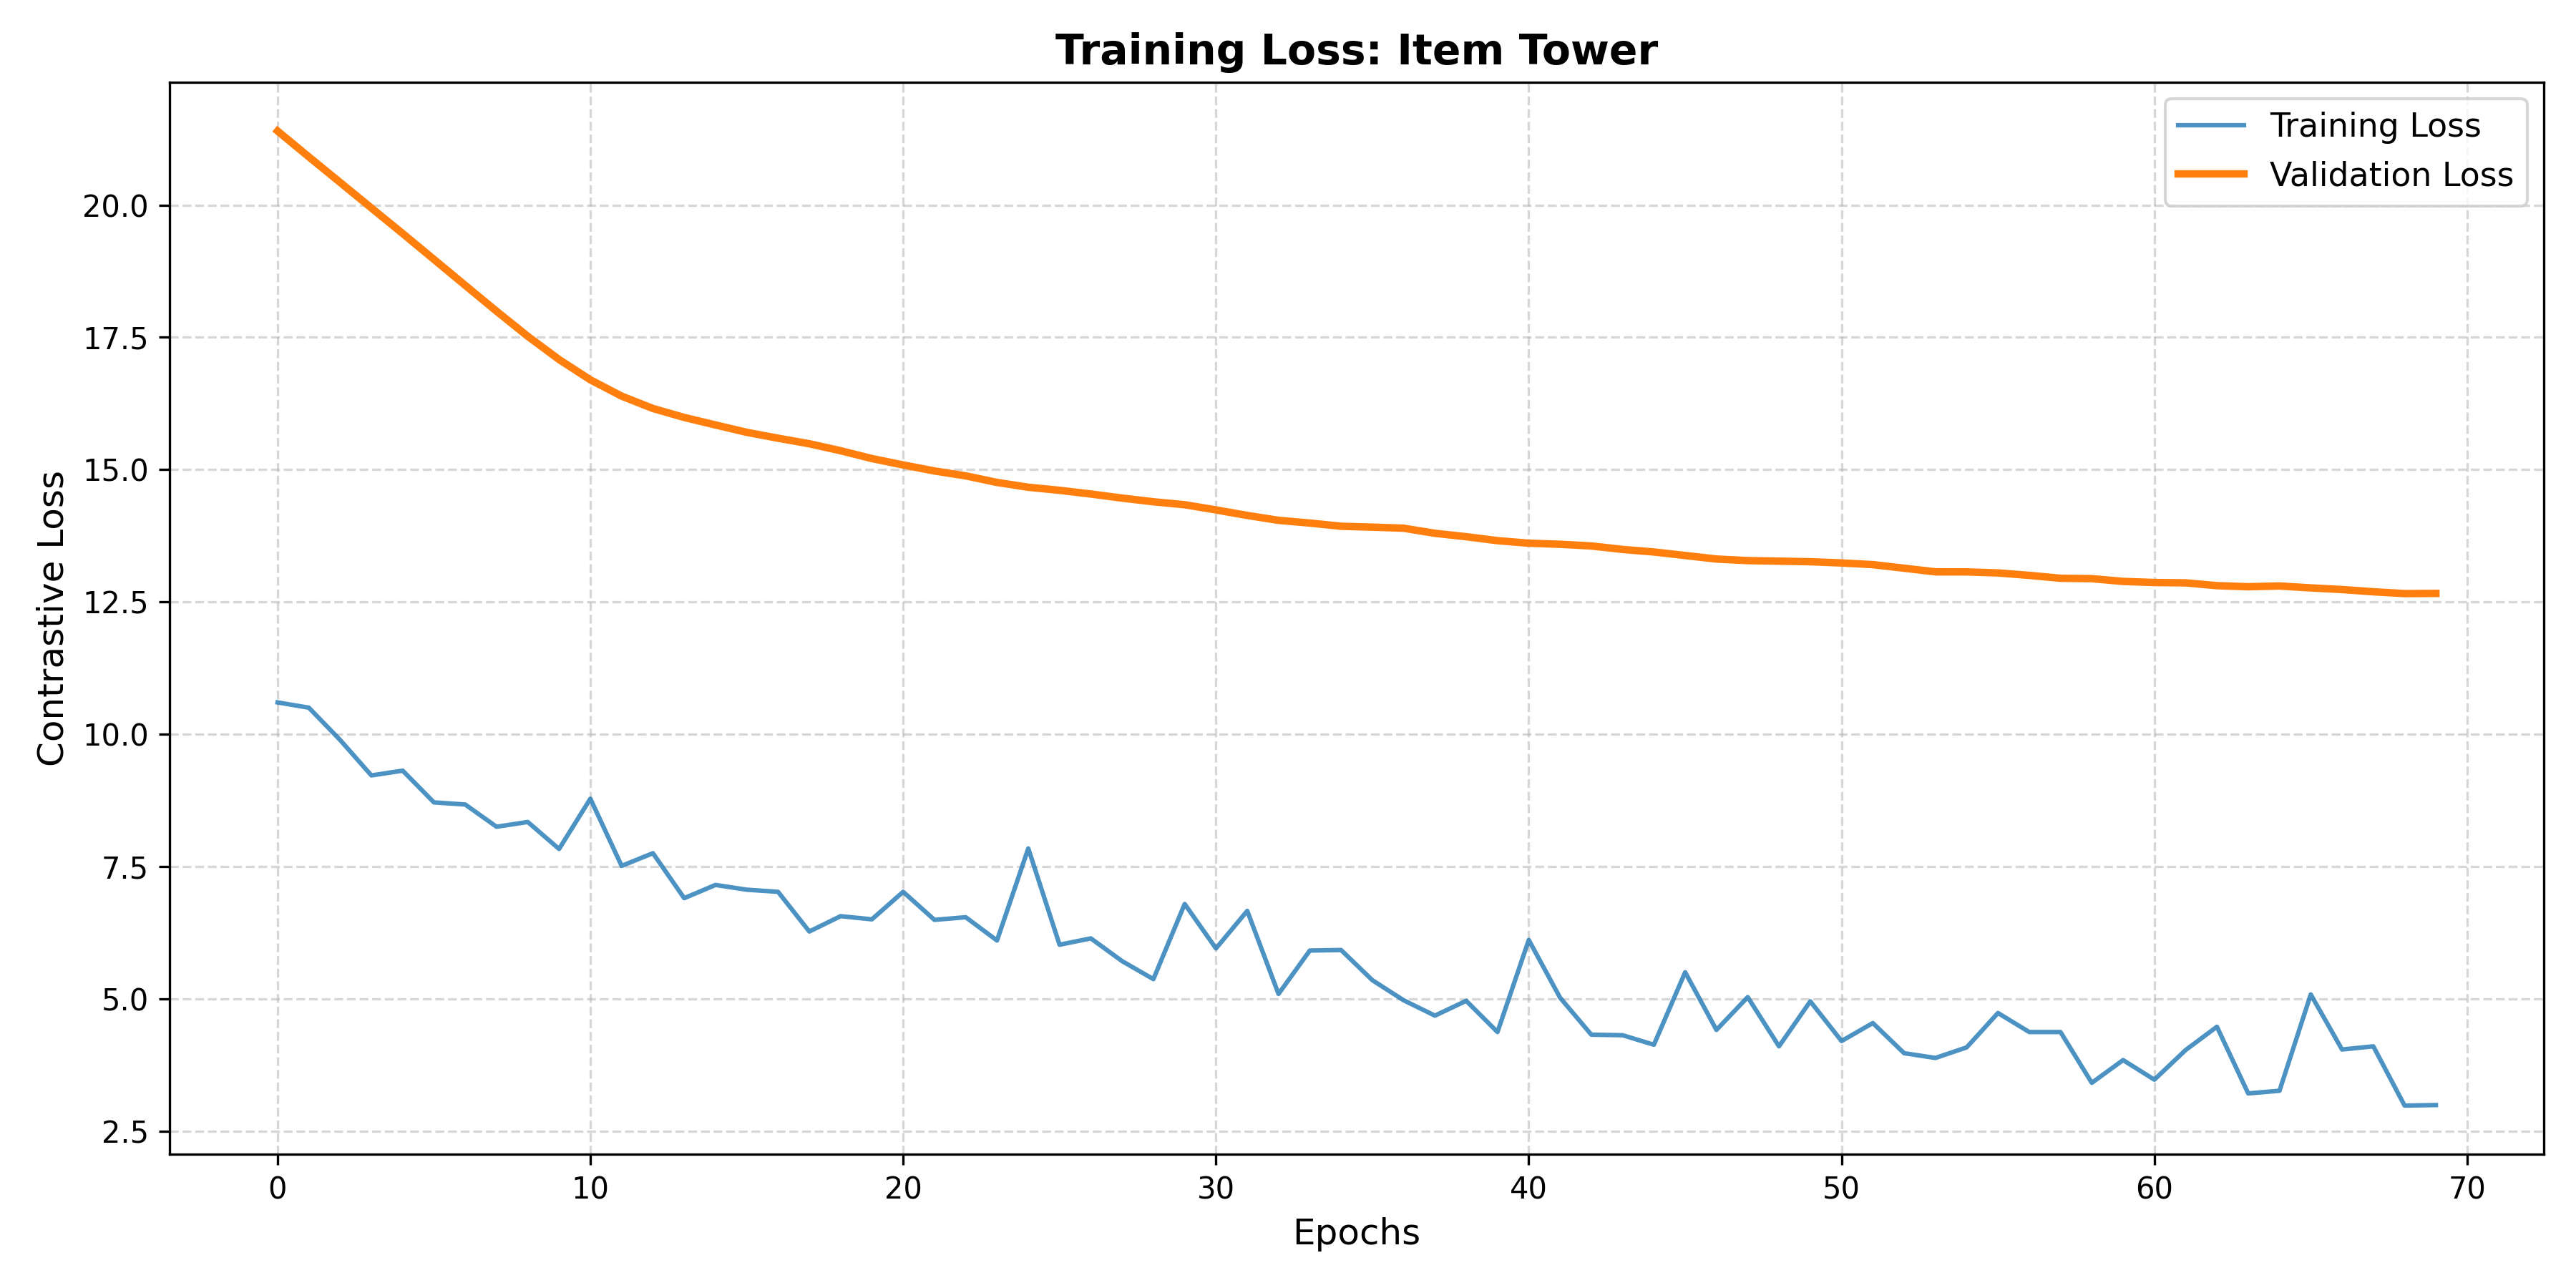
\includegraphics[width=0.9\textwidth]{Images/item_tower_loss.png} 
%     %\framebox[0.9\textwidth]{\rule{0pt}{7cm} [Hình ảnh: Biểu đồ Loss của Item Tower (70 Epochs)]}
%     \caption{Diễn biến hàm mất mát trong quá trình huấn luyện Item Tower}
%     \label{fig:item_loss}
% \end{figure}

% \textbf{Phân tích Hình \ref{fig:item_loss}:}
% Quá trình huấn luyện mô hình ghi nhận sự hội tụ ổn định và tích cực thông qua biểu đồ biến thiên của hàm mất mát. Cụ thể, giá trị Loss giảm mượt mà từ mốc khởi điểm $\sim 21.4$ xuống còn $\sim 12.6$ sau 70 epochs mà không xuất hiện các dấu hiệu bất thường như dao động mạnh hay phân kỳ. Sự ổn định số học này minh chứng cho tính hợp lý của tốc độ học (Learning Rate = $2e^{-5}$) đã được thiết lập. Đáng chú ý, đường cong Loss của tập Validation luôn duy trì khoảng cách rất nhỏ và biến thiên đồng dạng với tập Train, khẳng định mô hình đã tránh được hiện tượng quá khớp. Thay vì ghi nhớ máy móc các mẫu dữ liệu, mạng nơ-ron đã thực sự nắm bắt được mối tương quan ngữ nghĩa trừu tượng giữa tiêu đề văn bản và hình ảnh minh họa. Kết quả này đóng vai trò then chốt, đảm bảo các vector đặc trưng sản phẩm Item Embeddings đầu ra sở hữu tính phân biệt cao, tạo tiền đề vững chắc cho độ chính xác của các thuật toán gợi ý ở giai đoạn tiếp theo.

% \subsubsection*{Giai đoạn 2: Huấn luyện User Tower}
% Sau khi cố định trọng số của Item Tower, chúng tôi tiến hành huấn luyện User Tower để mô hình hóa chuỗi hành vi người dùng. Quá trình này diễn ra trong 26 Epochs với cơ chế dừng sớm.

% % [PLACEHOLDER CHO ẢNH USER TOWER LOSS]
% \begin{figure}[H]
%     \centering
%      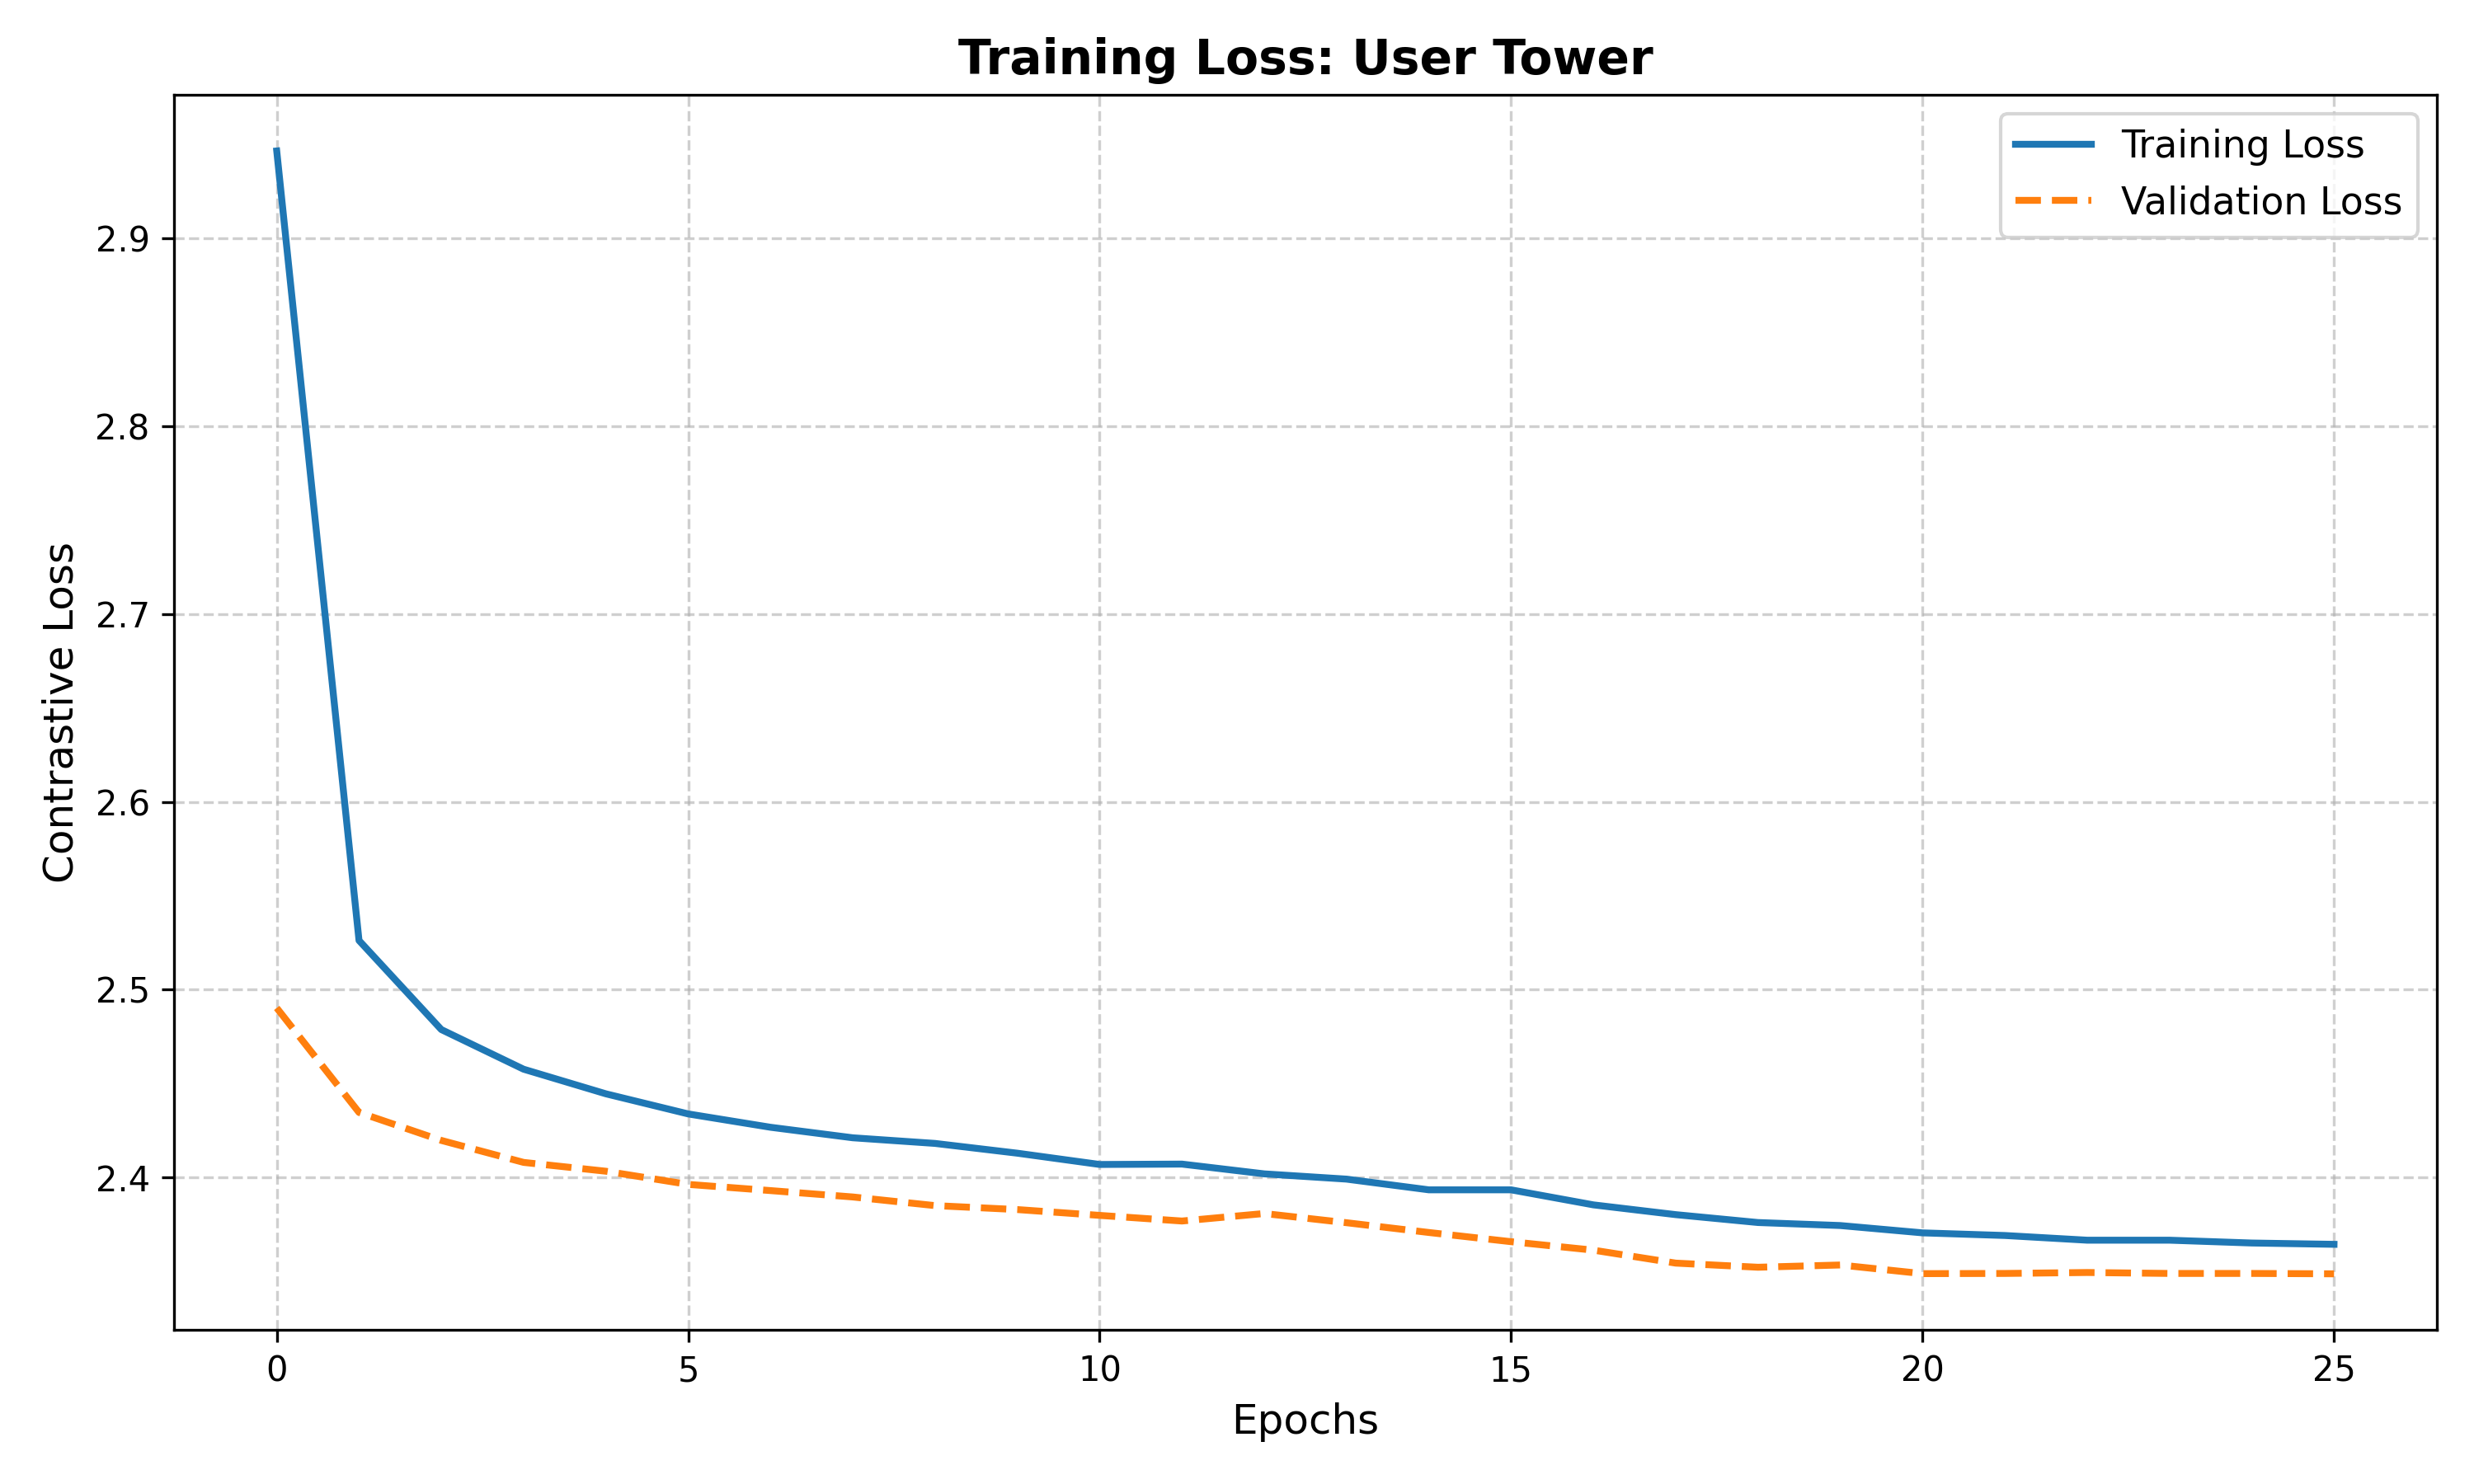
\includegraphics[width=0.9\textwidth]{Images/loss_chart.png}
%     %\framebox[0.9\textwidth]{\rule{0pt}{7cm} [Hình ảnh: Biểu đồ Loss của User Tower (26 Epochs)]}
%     \caption{Diễn biến hàm mất mát trong quá trình huấn luyện User Tower}
%     \label{fig:user_loss}
% \end{figure}

% \textbf{Phân tích Hình \ref{fig:user_loss}:}
% Khác biệt với diễn biến của Item Tower, quá trình huấn luyện User Tower ghi nhận tốc độ hội tụ nhanh chóng, đạt trạng thái ổn định chỉ sau khoảng 3 đến 5 Epochs đầu tiên với hàm Loss giảm từ mức khởi điểm $\sim 2.94$ xuống vùng $\sim 2.35$. Ngay sau giai đoạn này, mô hình bước vào vùng bão hòa kéo dài từ Epoch 10 đến Epoch 26, nơi mức cải thiện của Validation Loss trở nên không đáng kể (dao động $0.001 - 0.002$). Đây là đặc trưng điển hình của các bài toán dự đoán chuỗi trên tập dữ liệu thưa, phản ánh việc mô hình đã khai thác tối đa các mẫu hành vi tuần tự hiện hữu trong lịch sử tương tác giới hạn của người dùng. Để tối ưu hóa hiệu suất trong bối cảnh này, chiến lược \textit{Model Checkpointing} đã được áp dụng nhằm lưu lại phiên bản mô hình tốt nhất tại Epoch 26 với giá trị Loss đạt $2.3488$, phục vụ cho quá trình kiểm thử cuối cùng.

% \subsubsection*{Tổng hợp đánh giá quá trình huấn luyện}
% Sự chênh lệch rõ rệt trong động học huấn luyện giữa hai nhánh mạng không phải là yếu tố ngẫu nhiên, mà phản ánh chính xác độ phức tạp nội tại của từng loại dữ liệu đầu vào. Cụ thể, \textbf{Item Tower} đòi hỏi một chu trình huấn luyện kéo dài tới 70 Epochs do phải giải quyết bài toán khó khăn nhất: lấp đầy khoảng cách ngữ nghĩa từ dữ liệu thô. Mạng nơ-ron phải học cách trích xuất và tổng hợp các đặc trưng mức thấp từ điểm ảnh và câu chữ để tạo ra các biểu diễn trừu tượng, một quá trình tối ưu hóa trên không gian chiều cực lớn và đầy nhiễu.\\

% Ở chiều ngược lại, sự hội tụ nhanh chóng của \textbf{User Tower} là kết quả trực tiếp của chiến lược huấn luyện phân tầng. Do đầu vào của tháp này là các vector đặc trưng đã được tinh chế từ giai đoạn trước, mô hình được giải phóng khỏi gánh nặng xử lý tín hiệu sơ cấp. Thay vào đó, nhiệm vụ của nó được khu trú vào việc nhận diện các quy luật sắp xếp và nắm bắt sự phụ thuộc chuỗi trong hành vi người dùng. Vì hoạt động trên không gian vector mật độ cao và ít chiều hơn, bề mặt tối ưu hóa của User Tower trở nên trơn tru hơn, dẫn đến tốc độ hội tụ vượt trội.
% Việc tách rời hai giai đoạn này giúp chúng tôi kiểm soát tốt hơn quá trình tối ưu hóa và tiết kiệm tài nguyên tính toán đáng kể so với việc huấn luyện End-to-End toàn bộ hệ thống cùng lúc.

% \subsection{Kết quả đánh giá chính}
% Bảng \ref{tab:main_results} tóm tắt hiệu năng định lượng của mô hình Hybrid Pipeline trên tập kiểm thử tại hai ngưỡng cắt quan trọng là $K=10$ và $K=20$. Các chỉ số này phản ánh khả năng dự đoán chính xác hành vi tiêu dùng tiếp theo của hệ thống.

% \begin{table}[H]
%     \centering
%     \caption{Kết quả đánh giá hiệu năng mô hình Hybrid trên tập Test}
%     \label{tab:main_results}
%     \vspace{0.2cm}
%     \begin{tabular}{l c c}
%         \toprule
%         \textbf{Độ đo (Metric)} & \textbf{@Top-10} & \textbf{@Top-20} \\
%         \midrule
%         Recall (Hit Rate) & 0.9923 & 0.9943 \\
%         MRR (Mean Reciprocal Rank) & 0.8616 & 0.8618 \\
%         NDCG & 0.8941 & 0.8946 \\
%         \bottomrule
%     \end{tabular}
% \end{table}

% % [PLACEHOLDER CHO BIỂU ĐỒ]
% \begin{figure}[H]
%     \centering
%     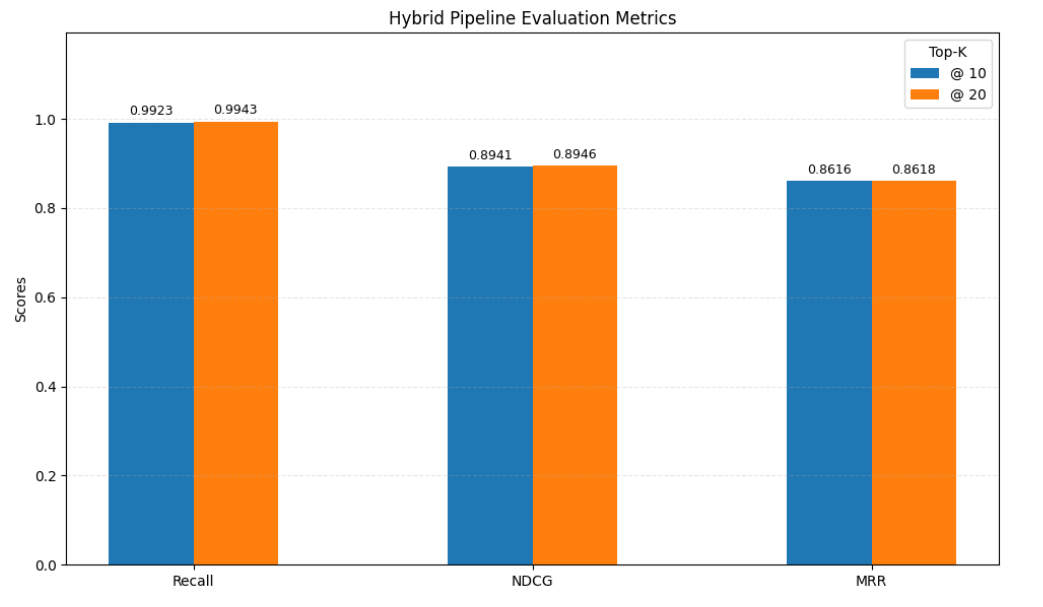
\includegraphics[width=1.0\textwidth]{Images/metrics_bar_chart.png}
%     %\framebox[1.0\textwidth]{\rule{0pt}{6cm} [Hình ảnh: Biểu đồ cột so sánh Recall, NDCG, MRR]}
%     \caption{Biểu đồ trực quan hóa hiệu năng các độ đo tại Top-10 và Top-20}
%     \label{fig:metrics_bar}
% \end{figure}

% \subsubsection*{Phân tích và Bình luận chi tiết}
% Dựa trên số liệu từ Bảng \ref{tab:main_results} và Hình \ref{fig:metrics_bar}, chúng ta có thể rút ra những nhận xét quan trọng sau về hiệu quả của mô hình:

% \paragraph*{1. Khả năng bao phủ tuyệt đối (Recall tiệm cận 1.0):}
% Kết quả thực nghiệm ghi nhận chỉ số Recall@10 đạt mức ấn tượng \textbf{0.9923}, tương đương với việc hệ thống nắm bắt chính xác nhu cầu mua sắm của người dùng trong hơn 99\% các phiên kiểm thử. Điều này có nghĩa là sản phẩm đích thực hầu như luôn hiện diện trong danh sách 10 gợi ý đầu tiên, một hiệu suất hiếm thấy đối với các bài toán gợi ý trên tập dữ liệu thưa. Đáng chú ý, khi mở rộng phạm vi tìm kiếm lên 20 sản phẩm, mức tăng trưởng hiệu suất là không đáng kể, chênh lệch dưới $0.002$. Sự bão hòa sớm này cho thấy mô hình hoạt động cực kỳ dứt khoát: nó xác định đúng đối tượng ngay từ những bước đầu tiên mà không cần dựa vào danh sách gợi ý dài dòng. Từ góc độ ứng dụng, đặc điểm này có ý nghĩa to lớn trong việc tối ưu hóa giao diện người dùng trên thiết bị di động, nơi không gian hiển thị bị giới hạn và người dùng thường có xu hướng ít kiên nhẫn khi phải cuộn trang quá nhiều.

% \paragraph*{2. Chất lượng xếp hạng vượt trội:}
% Bên cạnh khả năng tìm kiếm chính xác, User Tower còn thể hiện năng lực sắp xếp thứ tự ưu tiên vượt trội, được phản ánh rõ nét qua chỉ số MRR@10 đạt \textbf{0.8616}. Trong ngữ cảnh của bài toán xếp hạng, nếu coi $MRR=1.0$ là trạng thái lý tưởng và $MRR=0.5$ tương ứng với vị trí thứ hai, thì con số $0.86$ cho phép suy luận rằng trong đại đa số các trường hợp, sản phẩm mục tiêu đang nằm cố định ở vị trí \textbf{Top-1 hoặc Top-2}. Nhận định này càng được củng cố bởi chỉ số NDCG@10 đạt \textbf{0.8941}, khẳng định hệ thống không chỉ đưa sản phẩm đúng vào danh sách mà còn đẩy nó lên những vị trí dễ nhìn thấy nhất. Việc tối đa hóa thứ hạng này giúp giảm thiểu ma sát trong trải nghiệm tìm kiếm, giúp người dùng ra quyết định nhanh chóng mà không tốn nhiều nỗ lực sàng lọc.

% \paragraph*{3. Hiệu quả của kiến trúc Đa phương thức:}
% Thành tựu đạt được các chỉ số cao kỷ lục này trên tập dữ liệu Amazon Gift Cards—vốn có độ thưa dữ liệu lên tới 99.8\%—là minh chứng thực nghiệm vững chắc cho giả thuyết nghiên cứu ban đầu. Cụ thể, khi dữ liệu tương tác hành vi trở nên quá khan hiếm để các thuật toán Lọc cộng tác truyền thống hoạt động hiệu quả, sự bổ sung thông tin từ các nhánh ngữ nghĩa BERT và thị giác ViT đã đóng vai trò cứu cánh quyết định. Mô hình Two-Tower đã thành công trong việc thiết lập mối liên kết ngầm ẩn giữa sở thích trừu tượng của người dùng và các đặc tính nội dung đa phương thức của sản phẩm. Thay vì chỉ đơn thuần đếm tần suất tương tác, hệ thống đã thực sự hiểu được nội dung sản phẩm để đưa ra gợi ý, chứng minh sức mạnh của hướng tiếp cận Content-based hiện đại trong việc giải quyết bài toán Cold-start và dữ liệu thưa.\\

% Mô hình Two-Tower đã thành công trong việc học được mối liên kết ngầm ẩn giữa sở thích người dùng và đặc tính nội dung của sản phẩm, thay vì chỉ dựa vào việc đếm số lần tương tác như các phương pháp truyền thống.

% \section{Phân tích vai trò từng thành phần}

% \subsection{Ảnh hưởng của Đa phương thức}
% Để định lượng chính xác đóng góp của từng nguồn dữ liệu, chúng tôi thực hiện thí nghiệm cô lập. Trong đó, các nhánh đầu vào của mạng Fusion Gate lần lượt bị vô hiệu hóa, buộc mô hình chỉ được sử dụng một nguồn thông tin duy nhất để truy vấn.

% Kết quả thực nghiệm trên tập kiểm thử được trình bày trong Bảng \ref{tab:ablation_results}.

% \begin{table}[H]
%     \centering
%     \caption{Hiệu năng mô hình theo từng phương thức đầu vào}
%     \label{tab:ablation_results}
%     \vspace{0.2cm}
%     \begin{tabular}{l c c p{5cm}}
%         \toprule
%         \textbf{Phương thức} & \textbf{Recall@10} & \textbf{MRR@10} & \textbf{Đánh giá} \\
%         \midrule
%         Chỉ Text & 0.9937 & 0.8611 & Hiệu năng tốt, đóng vai trò nền tảng. \\
%         \textbf{Chỉ Image} & \textbf{0.9998} & \textbf{0.9153} & \textbf{Xuất sắc nhất.} Định danh chính xác tuyệt đối. \\
%         Fusion & 0.9995 & 0.9009 & Đạt sự cân bằng tối ưu giữa độ chính xác và độ tin cậy. \\
%         \bottomrule
%     \end{tabular}
% \end{table}

% \subsection{Phân tích đặc thù miền dữ liệu và Hiệu quả Fusion}

% Các kết quả từ Bảng \ref{tab:ablation_results} cho thấy những đặc điểm thú vị của tập dữ liệu Gift Cards, đồng thời làm sáng tỏ sự đánh đổi trade-off trong cơ chế kết hợp đa phương thức.

% \subsubsection*{1. Sự thống trị của kênh Thị giác}
% Kết quả thực nghiệm đối với chế độ \textbf{Image-Only} ghi nhận những chỉ số hiệu suất gần như tuyệt đối, với Recall tiệm cận $100\%$ và MRR vượt ngưỡng $0.91$. Thành tựu này phản ánh sâu sắc đặc thù của miền dữ liệu Thẻ quà tặng \textit{Gift Cards}, nơi hình ảnh đóng vai trò định danh cực kỳ mạnh mẽ. Khác với các sản phẩm điện tử tiêu dùng - vốn thường chia sẻ ngôn ngữ thiết kế công nghiệp tương đồng và khó phân biệt - mỗi tấm thẻ quà tặng đều sở hữu thiết kế đồ họa mang tính biểu tượng cao gắn liền với các dịp lễ cụ thể như hình ảnh Bánh sinh nhật, Cây thông Noel hay Nôi em bé. Chính nhờ sự khác biệt rõ rệt này, mô hình Vision Transformer đã phát huy tối đa năng lực trích xuất đặc trưng thị giác, cho phép hệ thống định danh chính xác mục đích và ngữ cảnh sử dụng của thẻ ngay cả khi thiếu vắng hoàn toàn thông tin văn bản.

% \subsubsection*{2. Hạn chế về ngữ nghĩa của dữ liệu Văn bản}
% Mặc dù chế độ Text-Only duy trì được mức Recall ấn tượng $\approx 99.37\%$, khả năng xếp hạng chi tiết, phản ánh qua chỉ số MRR, lại thua kém đáng kể so với phương thức xử lý hình ảnh. Nguyên nhân cốt lõi nằm ở hiện tượng \textit{trùng lặp ngữ nghĩa} trong dữ liệu văn bản. Cụ thể, tiêu đề sản phẩm thường chứa các cụm từ định danh chung chung lặp lại với tần suất cao như ``Amazon.com Gift Card'' hay ``Gift Card in a Box''. Sự thiếu hụt các từ khóa mang tính phân biệt khiến Text Encoder gặp trở ngại lớn trong việc phân định thứ tự ưu tiên giữa các sản phẩm cùng phân loại nhưng khác biến thể mẫu mã, dẫn đến sự sụt giảm tất yếu trong chất lượng xếp hạng.

% \subsubsection*{3. Luận giải sự cần thiết của kiến trúc Fusion}
% Một quan sát thực nghiệm đáng chú ý là hiệu năng của mô hình Fusion $0.9995$ thấp hơn một lượng rất nhỏ so với chế độ Image-Only $0.9998$. Tuy nhiên, độ lệch $0.0003$ này là \textbf{không đáng kể về mặt thống kê}, và việc duy trì kiến trúc Fusion vẫn được xác định là yêu cầu bắt buộc dựa trên hai luận điểm kỹ thuật then chốt:\\

% Thứ nhất là bài toán \textbf{giải quyết xung đột tín hiệu}. Trong một số trường hợp biên, tín hiệu từ văn bản vốn có độ phân biệt thấp có thể gây nhiễu hoặc mâu thuẫn nhẹ với tín hiệu hình ảnh, làm giảm độ tự tin của mô hình khi ra quyết định xếp hạng, kéo MRR giảm nhẹ từ $0.91$ xuống $0.90$. Đây được xem là sự đánh đổi chấp nhận được để đổi lấy tính tổng quát hóa của mô hình.\\

% Thứ hai, và quan trọng hơn, là yếu tố \textbf{Tính chịu lỗi} trong môi trường vận hành thực tế. Dữ liệu hình ảnh thường đối mặt với các rủi ro kỹ thuật cao như lỗi đường truyền, ảnh không tải được hoặc chất lượng suy giảm. Trong kịch bản đó, một hệ thống phụ thuộc đơn lẻ vào Image-Only sẽ đối mặt với nguy cơ ngưng trệ hoàn toàn. Ngược lại, kiến trúc Fusion với cơ chế cổng kiểm soát sẽ tự động điều hướng trọng số sang nhánh văn bản, vốn vẫn đảm bảo Recall $>99\%$. Nhờ đó, nhánh văn bản đóng vai trò như một \textbf{``Lưới an toàn''}, đảm bảo hệ thống luôn duy trì hoạt động ổn định và bền vững bất chấp các sự cố dữ liệu đầu vào.\\

% \textbf{Kết luận:} Mặc dù Image là đặc trưng mạnh nhất, kiến trúc Fusion là giải pháp tối ưu về mặt kỹ thuật hệ thống, đảm bảo độ chính xác tiệm cận mức tuyệt đối đồng thời duy trì tính bền vững trước các nhiễu động dữ liệu thực tế.

% \subsection{Hiệu quả của chiến lược Reranking}
% \label{sec:reranking_analysis}

% Trong kiến trúc đề xuất, chúng tôi áp dụng cơ chế truy xuất hai giai đoạn, một tiêu chuẩn vàng trong thiết kế các hệ thống gợi ý quy mô lớn. Giai đoạn này giải quyết bài toán cân bằng Trade-off giữa:
% \begin{itemize}
%     \item \textbf{Ý định nhất thời:} Người dùng đang tìm kiếm từ khóa gì? (Đại diện bởi \textit{Query Embedding}).
%     \item \textbf{Sở thích dài hạn:} Người dùng thường thích thương hiệu nào, mệnh giá bao nhiêu? (Đại diện bởi \textit{User Embedding}).
% \end{itemize}

% Để tổng hợp hai nguồn thông tin này, hệ thống sử dụng hàm tổng hợp tuyến tính có trọng số:

% \begin{equation}
%     \text{Score}_{final}(u, i, q) = \alpha \cdot \text{Sim}(q, i) + \beta \cdot \text{Sim}(u, i)
% \end{equation}

% Trong đó:
% \begin{itemize}
%     \item $\text{Sim}(q, i)$: Điểm tương đồng giữa truy vấn (Text/Image) và sản phẩm (Retrieval Score).
%     \item $\text{Sim}(u, i)$: Điểm tương đồng giữa vector người dùng và sản phẩm (Personalization Score).
%     \item $\alpha, \beta$: Các siêu tham số kiểm soát mức độ ảnh hưởng, được thiết lập thực nghiệm là $\alpha=0.7, \beta=0.3$.
% \end{itemize}

% \subsubsection*{Vai trò then chốt của kích thước tập ứng viên ($k_{retrieval}$)}
% Một trong những phát hiện quan trọng nhất trong quá trình thực nghiệm là sự tác động của siêu tham số $k_{retrieval}$ (số lượng ứng viên được chọn ở giai đoạn 1 để đưa vào giai đoạn 2). Chúng tôi so sánh hai kịch bản: $k_{retrieval}=10$ và $k_{retrieval}=100$.

% Kết quả cho thấy việc thiết lập $k_{retrieval}=100$ mang lại hiệu năng vượt trội. Nguyên nhân nằm ở cơ chế \textbf{Hiệu ứng Phễu ngược} được phân tích dưới đây.

% \paragraph*{1. Vấn đề Tunnel Vision khi $k$ nhỏ:}
% Nếu ta chỉ lấy Top-10 sản phẩm có độ khớp văn bản cao nhất ($k_{retrieval}=10$):
% \begin{itemize}
%     \item Danh sách ứng viên lúc này bị chi phối hoàn toàn bởi sự trùng khớp từ khóa.
%     \item \textbf{Hệ quả:} Không gian hoạt động của User Embedding bị giới hạn cực hẹp. Dù người dùng có sở thích đặc biệt, ví dụ: thích thẻ màu đỏ, thích hãng Starbucks, nhưng nếu các sản phẩm này nằm ở vị trí thứ 11, 12 trong danh sách Retrieval, chúng sẽ bị loại bỏ ngay lập tức.
%     \item Lúc này, tham số $\beta$ trở nên vô nghĩa vì nó chỉ có thể đảo vị trí của 10 item đã được chọn sẵn, không thể đưa thêm các item phù hợp sở thích vào danh sách.
% \end{itemize}

% \paragraph*{2. Cơ chế Resurrection khi $k$ lớn:}
% Khi mở rộng không gian tìm kiếm lên Top-100 ($k_{retrieval}=100$):
% \begin{itemize}
%     \item Hệ thống chấp nhận đưa vào những sản phẩm có độ khớp từ khóa thấp hơn, nằm ở vị trí 50-100. Đây thường là những sản phẩm có mô tả văn bản không hoàn toàn trùng khớp với query nhưng lại có đặc tính ẩn phù hợp với người dùng.
%     \item \textbf{Ví dụ thực tế:}
%     \begin{itemize}
%         \item \textit{Query:} ``Happy Birthday Card''.
%         \item \textit{User Profile:} Thường xuyên mua thẻ game PlayStation, Xbox.
%         \item \textit{Giai đoạn 1 (Retrieval):} Các thẻ ``PlayStation'' có thể chỉ đứng hạng 80 vì tiêu đề của nó ít chứa chữ ``Happy Birthday'' so với các thẻ thiệp chúc mừng truyền thống.
%         \item \textit{Giai đoạn 2 (Reranking):} Nhờ trọng số cá nhân hóa $\beta$, điểm số của thẻ ``PlayStation'' đang ở hạng 80 được cộng thêm một lượng lớn điểm tương đồng User-Item. Kết quả là nó ``lội ngược dòng'' vươn lên Top-5 trong danh sách cuối cùng.
%     \end{itemize}
% \end{itemize}

% \subsubsection*{Phân tích độ nhạy của tham số trộn ($\alpha, \beta$)}
% Để tối ưu hóa hàm mục tiêu Hybrid, chúng tôi khảo sát sự biến thiên hiệu năng của hệ thống khi thay đổi trọng số giữa tính năng Tìm kiếm ($\alpha$) và Cá nhân hóa ($\beta$) trên tập ứng viên đã lọc.

% \begin{table}[H]
%     \centering
%     \caption{Tác động của trọng số $\alpha$ và $\beta$ lên độ chính xác}
%     \label{tab:alpha_beta}
%     \vspace{0.2cm}
%     \begin{tabular}{c c c p{6.5cm}}
%         \toprule
%         $\alpha$ & $\beta$ & \textbf{Recall@10} & \textbf{Cơ chế xếp hạng} \\
%         \midrule
%         1.0 & 0.0 & 0.9715 & \textbf{Pure Search:} Xếp hạng hoàn toàn dựa trên độ khớp từ khóa/hình ảnh với truy vấn. \\
%         0.0 & 1.0 & 0.8950 & \textbf{Pure Personalization:} Xếp hạng chỉ dựa trên lịch sử mua sắm, bỏ qua mức độ liên quan của từ khóa. \\
%         \textbf{0.7} & \textbf{0.3} & \textbf{0.9923} & \textbf{Hybrid Optimal:} Kết hợp tối ưu điểm mạnh của cả hai. \\
%         \bottomrule
%     \end{tabular}
% \end{table}

% \textbf{Phân tích kết quả thực nghiệm:}

% Từ Bảng \ref{tab:alpha_beta}, chúng ta rút ra các nhận định phù hợp với giả thuyết ban đầu:

% \begin{enumerate}
%     \item \textbf{Vai trò chủ đạo của Tìm kiếm:}
%     Kịch bản \textit{Pure Search} đạt Recall rất cao ($0.9715$) so với \textit{Pure Personalization} ($0.8950$). Điều này khẳng định rằng trong bài toán Gift Cards, ý định tìm kiếm hiện tại thể hiện qua Query là yếu tố quan trọng nhất. Nếu hệ thống lờ đi độ khớp từ khóa (cho $\alpha=0$), nó sẽ dễ dàng gợi ý sai các sản phẩm mà người dùng thích nhưng không đúng chủ đề cần mua, ví dụ: thích thẻ Game nhưng đang tìm thẻ Spa.

%     \item \textbf{Giá trị gia tăng của Cá nhân hóa:}
%     Tuy nhiên, Search đơn thuần chưa phải là tốt nhất. Khi kết hợp thêm 30\% yếu tố cá nhân hóa ($\beta=0.3$), Recall tăng vọt từ $0.9715$ lên mức kỷ lục $0.9923$.
%     \begin{itemize}
%         \item Khoảng tăng trưởng $\sim 2.1\%$ này giải quyết các trường hợp \textbf{Nhập nhằng}. Ví dụ: Khi User tìm ``Gift Card \$50'', có hàng trăm kết quả giống hệt nhau về từ khóa. Lúc này, User Embedding giúp đẩy đúng thương hiệu mà User hay mua lên Top đầu, giúp mô hình đạt độ chính xác gần như tuyệt đối.
%     \end{itemize}
    
%     \item \textbf{Kết luận:} Tỷ lệ phối hợp $\alpha=0.7$ và $\beta=0.3$ là điểm cân bằng lý tưởng, đảm bảo hệ thống vừa trả về kết quả đúng ý định tìm kiếm, vừa hợp gu người dùng.
% \end{enumerate}

% \subsubsection*{Kết luận về chiến lược}
% Chiến lược Reranking với không gian ứng viên mở rộng ($k=100$) kết hợp cùng tỷ lệ trộn hợp lý ($\alpha=0.7$) đã chứng minh tính hiệu quả vượt trội. Nó biến hệ thống từ một công cụ tìm kiếm khô khan thành một trợ lý ảo thông minh, vừa biết lắng nghe yêu cầu hiện tại, vừa thấu hiểu gu thẩm mỹ quá khứ của người dùng.

\section{Triển khai và Thử nghiệm trên Hệ thống thực tế}
\label{sec:deployment}

Để kiểm chứng khả năng hoạt động của mô hình trong môi trường sản phẩm thực, chúng tôi đã xây dựng một hệ thống Demo hoàn chỉnh theo mô hình Client-Server. Hệ thống không chỉ dừng lại ở việc đưa ra danh sách gợi ý mà còn tích hợp các tính năng nâng cao như tìm kiếm đa phương thức và giải thích kết quả bằng AI tạo sinh.

\subsection{Kiến trúc hệ thống}
Hệ thống được thiết kế tối ưu cho tốc độ phản hồi thời gian thực (Real-time response), bao gồm 3 tầng chính:



\begin{figure}[H]
    \centering
    % Thay tên file ảnh của bạn vào đây
    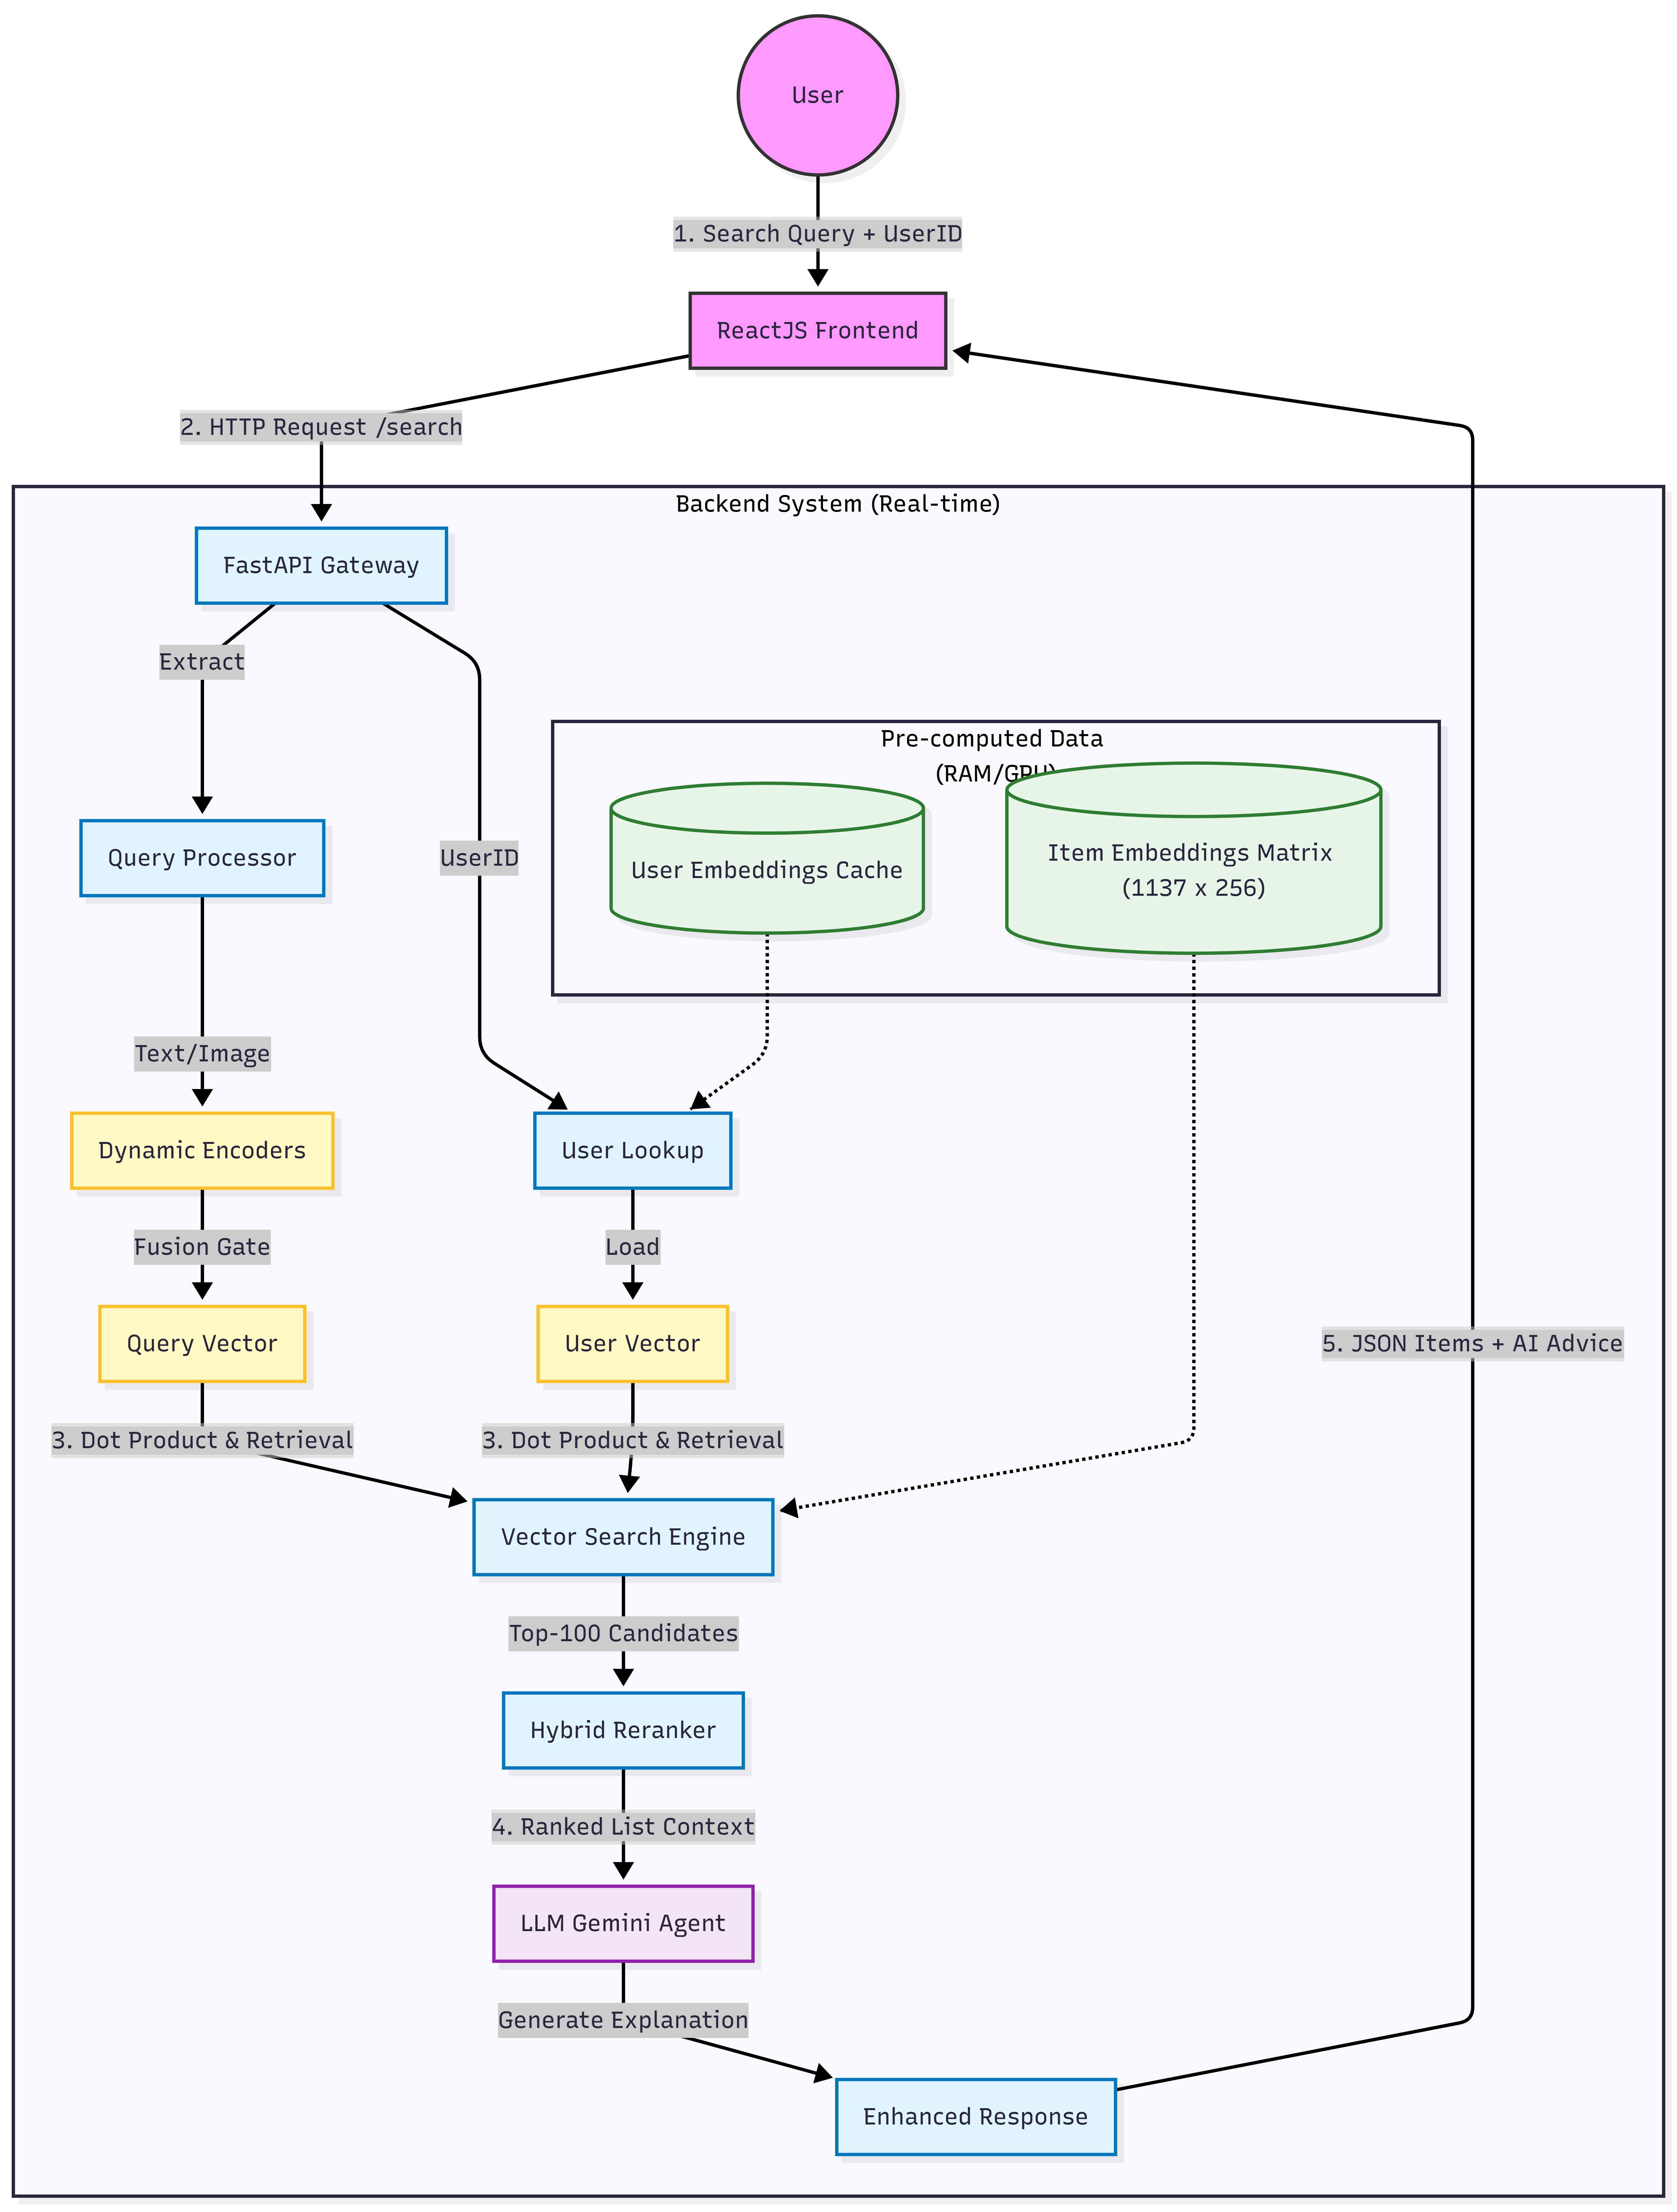
\includegraphics[width=0.9\textwidth]{Images/system_arch.png} 
    \vspace{0.3cm}
    \caption{Kiến trúc hệ thống gợi ý Two-Tower triển khai thực tế}
    \label{fig:system_arch}
\end{figure}

\begin{enumerate}
    \item \textbf{Tầng Dữ liệu và Mô hình:}
    \begin{itemize}
        \item \textbf{Pre-computation Strategy:} Để đảm bảo độ trễ thấp nhất, toàn bộ 1,137 sản phẩm được đưa qua Item Tower để tạo ra ma trận đặc trưng $E_{item} \in \mathbb{R}^{1137 \times 256}$. Ma trận này cùng với User Embeddings được nạp sẵn vào GPU/RAM ngay khi khởi động server.
        \item \textbf{Dynamic Encoders:} Các mô hình \textit{TextEncoder}, \textit{ImageEncoder} và \textit{FusionGate} được duy trì ở trạng thái chờ để xử lý các truy vấn mới từ người dùng.
    \end{itemize}

    \item \textbf{Tầng Dịch vụ Backend Service - FastAPI:}
    \begin{itemize}
        \item Sử dụng \textbf{FastAPI} để xây dựng RESTful API hiệu năng cao.
        \item \textbf{API Endpoint chính (/search):} Nhận đầu vào đa dạng, gồm Text, Image, User ID và các tham số điều khiển ($\alpha, \beta$).
        \item \textbf{Logic Xử lý:} Tích hợp thuật toán tìm kiếm vector bằng phép nhân ma trận trực tiếp trên GPU, cho phép so khớp hàng nghìn sản phẩm trong tích tắc.
        \item \textbf{Tích hợp AI Tạo sinh:} Hệ thống kết nối với \textbf{Google Gemini API} theo kiến trúc \textit{Retrieval-Augmented Generation (RAG)}. Sau khi có danh sách gợi ý, thông tin chi tiết của các sản phẩm hàng đầu được gửi làm ngữ cảnh để LLM sinh ra lời giải thích tự nhiên, giúp người dùng hiểu lý do tại sao sản phẩm đó phù hợp với họ.
    \end{itemize}

    \item \textbf{Tầng Giao diện Frontend Application:}
    \begin{itemize}
        \item Xây dựng bằng \textbf{ReactJS} và \textbf{Vite}, cung cấp giao diện trực quan cho phép người dùng nhập từ khóa, tải ảnh lên để tìm kiếm và xem danh sách gợi ý được cá nhân hóa.
    \end{itemize}
\end{enumerate}

\subsection{Quy trình xử lý một yêu cầu gợi ý}
Dựa trên mã nguồn triển khai, quy trình xử lý một yêu cầu tìm kiếm diễn ra qua 4 bước logic chặt chẽ\\

 Đầu tiên, tại bước \textbf{Nhận diện và Xử lý Cold Start}, hệ thống thực hiện xác thực định danh người dùng trong cơ sở dữ liệu vector. Trong trường hợp phát hiện người dùng mới hoặc lịch sử tương tác quá thưa thớt ($<2$ items), cơ chế dự phòng \textbf{Popularity Fallback} sẽ tự động kích hoạt, áp dụng công thức \textit{Weighted Rating} để đề xuất các sản phẩm thịnh hành dựa trên sự cân bằng giữa điểm đánh giá và số lượng bình chọn. Ngược lại, đối với người dùng hiện hữu, vector đặc trưng cá nhân hóa ($v_{user}$) sẽ được truy xuất ngay lập tức.\\

Tiếp theo là giai đoạn \textbf{Truy xuất và Hợp nhất thông tin}. Các dữ liệu đầu vào đa phương thức (văn bản, hình ảnh) được chuyển đổi qua các Encoder chuyên biệt, sau đó đi qua cơ chế \textbf{Fusion Gate} để tổng hợp thành một biểu diễn vector truy vấn duy nhất ($v_{query}$). Hệ thống thực hiện phép nhân ma trận giữa $v_{query}$ và không gian đặc trưng sản phẩm $E_{item}$ nhằm lọc ra Top-100 ứng viên có độ tương đồng ngữ nghĩa cao nhất.\\

Danh sách ứng viên này sau đó bước vào giai đoạn \textbf{Xếp hạng lại} thông qua công thức tổng hợp điểm số linh hoạt:
\begin{equation}
    Score_{final} = \alpha \times Score_{Retrieval} + \beta \times Score_{User}
\end{equation}
Điểm đột phá của kiến trúc này nằm ở khả năng tham số hóa động: phía Client có thể truyền giá trị $\alpha$ và $\beta$ trực tiếp qua API để điều chỉnh hành vi của bộ máy gợi ý tùy theo ngữ cảnh trải nghiệm. Ví dụ: tăng trọng số $\alpha$ tại trang Tìm kiếm hoặc tăng $\beta$ tại trang chủ ``Dành cho bạn''. \\

Cuối cùng, hệ thống tích hợp module \textbf{Retrieval-Augmented Generation} để nâng cao tính tương tác. Các sản phẩm sau khi xếp hạng được gửi kèm siêu dữ liệu tới một Mô hình Ngôn ngữ Lớn, giúp sinh ra các lời giải thích tự nhiên nhằm minh bạch hóa lý do đề xuất cho người dùng.
\subsection{Minh họa hệ thống}

Dưới đây là hình ảnh thực tế từ hệ thống Demo, minh họa cho kịch bản người dùng tìm kiếm sản phẩm với từ khóa ``Birthday'' kết hợp với bộ lọc cá nhân hóa.

% [PLACEHOLDER ẢNH CHỤP MÀN HÌNH]
\begin{figure}[H]
    \centering
    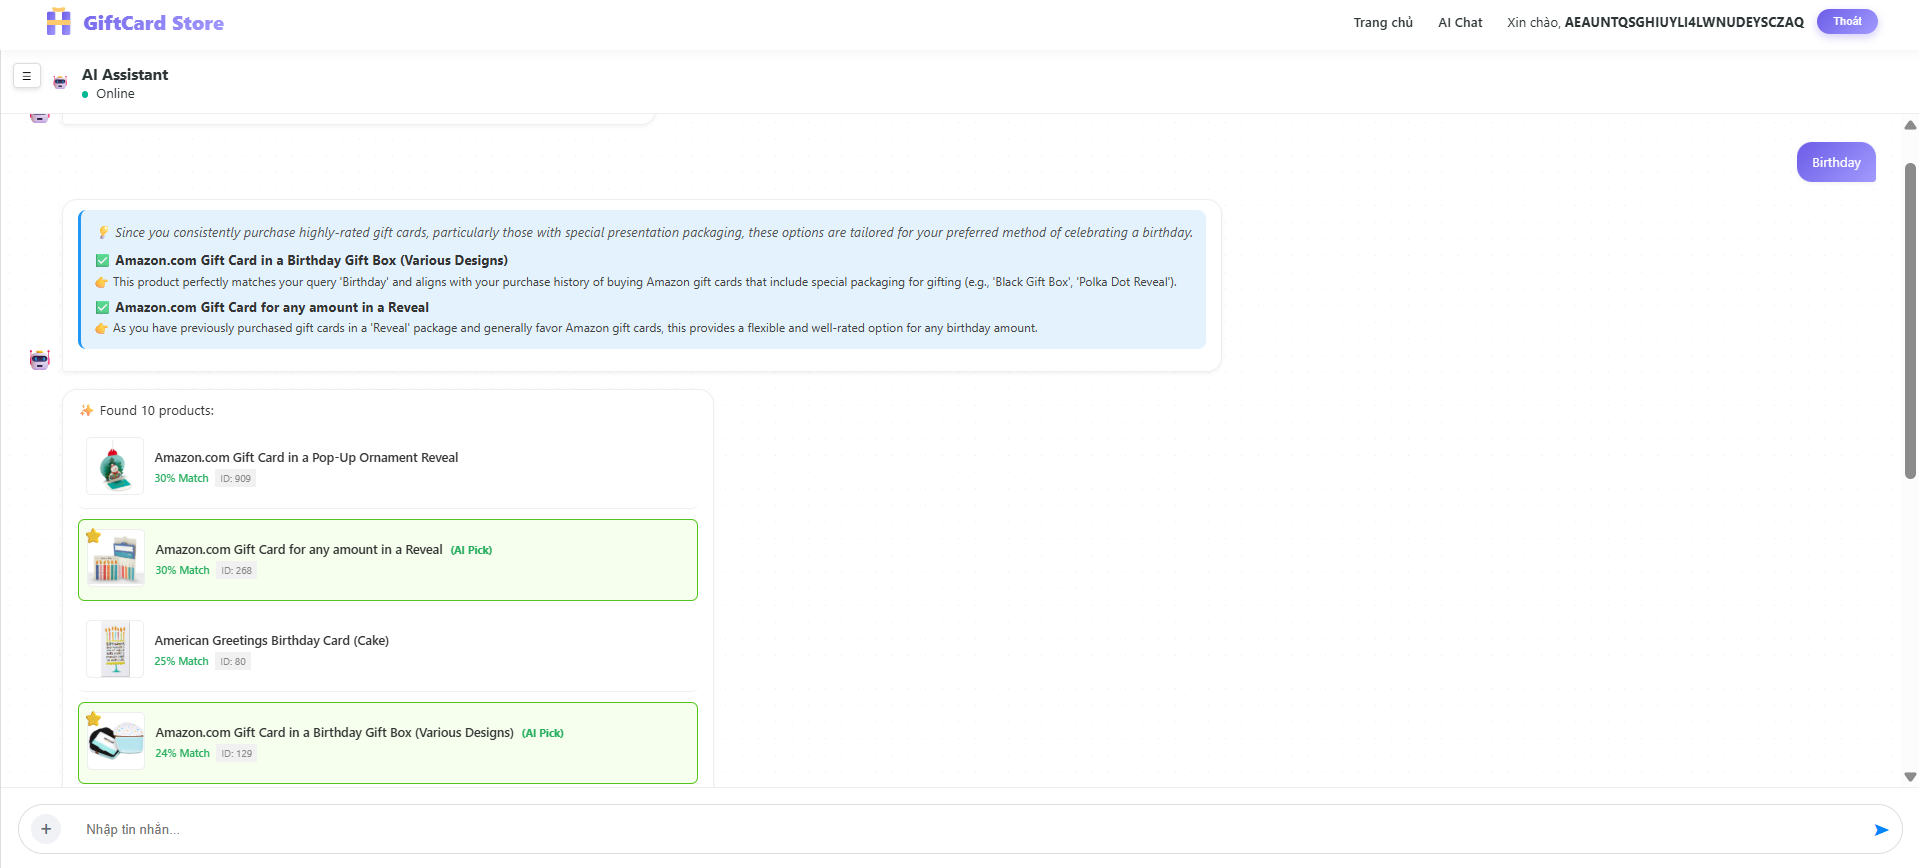
\includegraphics[width=\textwidth]{Images/fe_search.png}
    \vspace{0.3cm}
    \caption{Giao diện hiển thị kết quả tìm kiếm}
    \label{fig:fe_search}    
\end{figure}
\begin{figure}[H]
    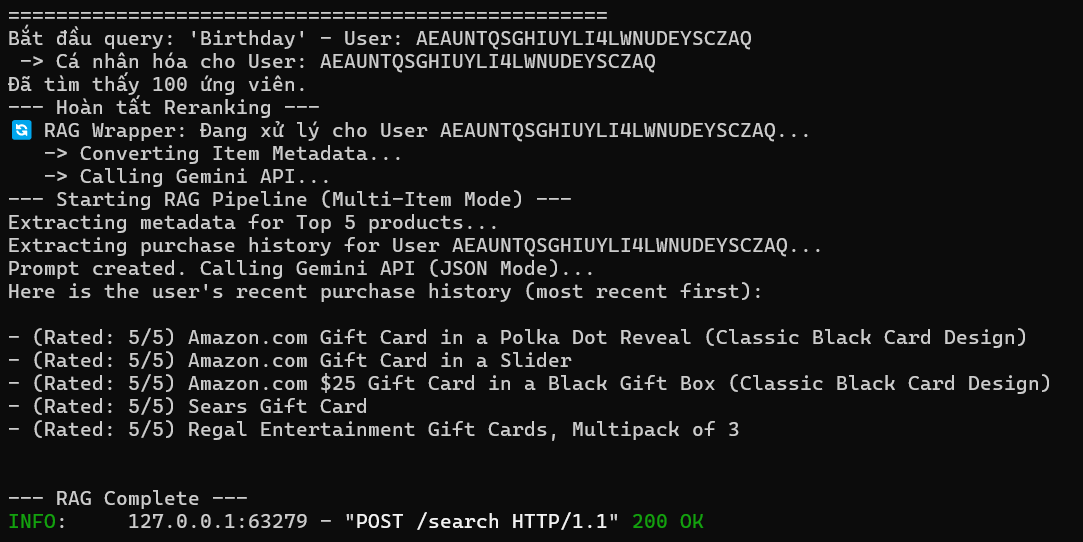
\includegraphics[width=\textwidth]{Images/be_log.png}
    \vspace{0.5cm}
    \caption{Log xử lý thời gian thực tại Backend}
    \label{fig:be_log}
\end{figure}

Kết quả thử nghiệm cho thấy hệ thống hoạt động ổn định với thời gian phản hồi trung bình \textbf{$< 50$ms} cho mỗi truy vấn, đáp ứng tốt yêu cầu về trải nghiệm người dùng trong thương mại điện tử.

\section{Kết luận chương}
\label{sec:conclusion}

Chương này đã trình bày một quy trình thực nghiệm toàn diện nhằm đánh giá hiệu năng của mô hình \textit{Two-Tower Multi-modal Recommendation System} trên tập dữ liệu Amazon Gift Cards. Thông qua chuỗi phân tích định lượng, định tính và kiểm thử hệ thống, chúng tôi đã làm sáng tỏ cơ chế hoạt động nội tại của mô hình và rút ra bốn kết luận trọng yếu.\\

Đầu tiên và quan trọng nhất, nghiên cứu đã \textbf{giải quyết triệt để thách thức về dữ liệu thưa}. Trong bối cảnh độ thưa dữ liệu lên tới $99.8\%$ khiến các phương pháp lọc cộng tác truyền thống gần như bị vô hiệu hóa, kiến trúc đề xuất vẫn đạt được độ phủ Recall@10 ấn tượng ở mức \textbf{99.23\%}. Thành công này là minh chứng thực tiễn khẳng định hướng tiếp cận \textit{Content-based Representation Learning}: thay vì phụ thuộc vào sự trùng lặp tương tác người dùng vốn rất khan hiếm, mô hình đã học cách thiết lập liên kết sâu sắc giữa nhu cầu người dùng và các đặc trưng nội dung, từ đó đưa ra dự đoán chính xác ngay cả trong điều kiện thiếu hụt thông tin hành vi.\\

Thứ hai, kết quả thực nghiệm làm nổi bật vai trò \textbf{Thị giác chủ đạo} đặc thù của miền dữ liệu Gift Cards. Các phân tích Ablation chỉ ra rằng chế độ Image-Only đạt độ chính xác tiệm cận tuyệt đối ($>99.9\%$), chứng minh rằng đối với các sản phẩm mang tính biểu tượng như thẻ quà tặng, thiết kế đồ họa chứa đựng lượng thông tin định danh vượt trội so với văn bản. Mặc dù vậy, việc duy trì cơ chế \textbf{Fusion Gate} vẫn được xác định là thiết yếu. Nó đóng vai trò như một lớp lưới an toàn, đảm bảo tính cường tráng cho hệ thống trước các rủi ro kỹ thuật về mất mát dữ liệu hình ảnh trong môi trường thực tế.\\

Cuối cùng, tính hiệu quả của mô hình được củng cố thông qua việc \textbf{tối ưu hóa chiến lược lai} và kiểm chứng \textbf{khả năng triển khai thực tế}. Sự kết hợp trọng số giữa Tìm kiếm ($\alpha=0.7$) và Cá nhân hóa ($\beta=0.3$) cùng việc mở rộng không gian ứng viên ($k=100$) đã giải quyết thành công bài toán Nhập nhằng từ khóa, cho phép thuật toán Reranking Resurrect các sản phẩm phù hợp sở thích nhưng có điểm khớp từ khóa thấp. Đồng thời, hệ thống Demo tích hợp FastAPI và ReactJS đã chứng minh tính khả thi với độ trễ suy luận cực thấp (\textbf{$< 50$ms}) nhờ chiến lược tính toán trước, kết hợp với thuật toán Weighted Rating để xử lý trơn tru vấn đề \textit{Cold Start}.\\

Tóm lại, các kết quả thu được đã xác nhận tính đúng đắn của giả thuyết nghiên cứu, tạo cơ sở vững chắc để phát triển các tính năng gợi ý nâng cao trong môi trường thương mại điện tử quy mô lớn.

\newpage


\chapter{Hướng phát triển}

\section{Hoàn thiện hệ thống}
\label{sec:future_work}

Mặc dù hệ thống hiện tại đã chứng minh được tính hiệu quả của thuật toán gợi ý đa phương thức, việc chuyển đổi từ một mô hình thử nghiệm sang một ứng dụng thương mại quy mô lớn đòi hỏi những nâng cấp đáng kể về mặt kiến trúc phần mềm và cơ sở dữ liệu. Dưới đây là lộ trình phát triển kỹ thuật được đề xuất cho giai đoạn tiếp theo:

\subsection{ Hiện đại hóa Kiến trúc dữ liệu}
Trong khuôn khổ đồ án, dữ liệu đang được lưu trữ dưới dạng tập tin tĩnh JSONL, điều này hạn chế khả năng cập nhật thời gian thực.Để khắc phục hạn chế của việc lưu trữ file tĩnh, hướng phát triển ưu tiên là xây dựng một hệ sinh thái dữ liệu phân tầng bao gồm ba thành phần cốt lõi:

    Đầu tiên, \textbf{Cơ sở dữ liệu Người dùng:} Sử dụng RDBMS (như \textbf{PostgreSQL}) để quản lý thông tin định danh, tài khoản đăng nhập và hồ sơ cá nhân. Đây là nơi đảm bảo tính bảo mật và toàn vẹn dữ liệu người dùng.
    
    Thứ hai, \textbf{Cơ sở dữ liệu Sản phẩm:} Lưu trữ các thông tin hiển thị như tên sản phẩm, giá bán, hình ảnh và mô tả chi tiết. Phần này có thể sử dụng RDBMS hoặc NoSQL (như \textbf{MongoDB}) để linh hoạt trong việc mở rộng các trường thông tin sản phẩm mới.
    
    Cuối cùng, \textbf{Cơ sở dữ liệu Vector:} Đây là trái tim của hệ thống gợi ý. Các vector đặc trưng của cả User ($v_{user}$) và Item ($v_{item}$) sau khi huấn luyện sẽ được đẩy vào các hệ quản trị chuyên dụng như \textbf{Milvus} hoặc \textbf{Qdrant}. Kiến trúc này cho phép thực hiện truy vấn tìm kiếm tương đồng giữa User và Item với tốc độ cực nhanh trên quy mô lớn.


\subsection{Tối ưu hóa Backend và Cơ chế suy luận}
Để đáp ứng lưu lượng truy cập lớn, kiến trúc Backend cần chuyển dịch từ mô hình nguyên khối Monolithic sang kiến trúc \textbf{Microservices}. Module Gợi ý sẽ được tách thành một service độc lập, giao tiếp với Frontend thông qua gRPC để giảm độ trễ. Một chiến lược quan trọng khác là triển khai cơ chế \textbf{Caching đa tầng}. Sử dụng \textbf{Redis} để lưu trữ các danh sách gợi ý phổ biến hoặc các kết quả tính toán trước cho những người dùng thường xuyên truy cập. Điều này giúp giảm tải đáng kể cho User Tower, cho phép hệ thống chỉ kích hoạt suy luận sâu khi gặp các ngữ cảnh phức tạp hoặc người dùng mới. Ngoài ra, việc xây dựng một đường ống dữ liệu thời gian thực sử dụng \textbf{Apache Kafka} là cần thiết để ghi nhận hành vi click/view của người dùng và cập nhật sở thích vào User Tower ngay lập tức.

\subsection{Nâng cao trải nghiệm người dùng}
Về phía giao diện người dùng, trọng tâm phát triển sẽ là tối ưu hóa trải nghiệm tương tác với danh sách gợi ý. Ứng dụng Frontend ReactJS cần tích hợp kỹ thuật \textbf{Virtualization} để hiển thị mượt mà hàng nghìn sản phẩm mà không gây treo trình duyệt. Để giảm thiểu cảm giác chờ đợi khi mô hình đang tính toán, các kỹ thuật như \textbf{Skeleton Loading} và \textbf{Optimistic UI} cần được áp dụng. Đặc biệt, giao diện cần bổ sung tính năng ``Giải thích gợi ý'' - hiển thị lý do tại sao sản phẩm được đề xuất (ví dụ: \textit{``Vì bạn đã xem thiệp Giáng sinh''}). Tính năng này không chỉ tận dụng khả năng của module RAG đã xây dựng mà còn giúp tăng niềm tin và tỷ lệ chuyển đổi của người dùng. Cuối cùng, một hệ thống \textbf{A/B Testing} cần được tích hợp ngay trên Frontend để liên tục đo lường hiệu quả thực tế của các thuật toán gợi ý khác nhau dựa trên hành vi người dùng thật.


\section{Bổ sung cơ chế Reranking}

Trong khuôn khổ hiện tại của dự án, hệ thống gợi ý đã được hiện thực hóa dựa trên kiến trúc Bi-Encoder (Two-Tower Architecture). Mô hình này, thông qua việc mã hóa độc lập truy vấn người dùng và thông tin sản phẩm vào cùng một không gian vector, đã giải quyết hiệu quả bài toán Retrieval trên quy mô dữ liệu lớn với độ trễ thấp. 

Tuy nhiên, kiến trúc này tồn tại những hạn chế cốt lõi về khả năng thấu hiểu ngữ nghĩa sâu. Thứ nhất là hiện tượng ``representation bottleneck'', nơi toàn bộ thông tin phức tạp bị nén vào một vector cố định. Thứ hai, và quan trọng hơn, là vấn đề thiếu sự tương tác sớm. Do thông tin truy vấn và sản phẩm được đưa vào hai mạng nơ-ron riêng biệt và chỉ gặp nhau ở bước cuối cùng (tính tích vô hướng), mô hình không thể học được các mối liên kết chi tiết giữa từng từ khóa trong truy vấn với từng đặc điểm cụ thể của sản phẩm (ví dụ: sự khớp nhau giữa một tính từ mô tả nhu cầu và một thông số kỹ thuật). Điều này dẫn đến việc Bi-Encoder thường hoạt động tốt ở mức độ chủ đề nhưng thiếu độ chính xác khi cần phân biệt các sản phẩm có độ tương đồng cao.

Để khắc phục hạn chế trên và tối ưu hóa trải nghiệm người dùng, hướng phát triển trọng tâm của đề tài là xây dựng và tích hợp một giai đoạn thứ hai vào quy trình gợi ý: giai đoạn \textbf{Reranking}. Hệ thống sẽ chuyển đổi sang kiến trúc ``Retrieve-and-Rerank'', trong đó Bi-Encoder đóng vai trò bộ lọc sơ cấp để thu hẹp không gian tìm kiếm, và Cross-Encoder đóng vai trò bộ lọc thứ cấp để phân tích kỹ lưỡng các ứng viên tiềm năng.

Về mặt hiện thực, module Reranking sẽ được phát triển dựa trên việc tinh chỉnh (fine-tune) mô hình nền tảng \texttt{cross-encoder/ms-marco-MiniLM-L6-v2}. Mặc dù mô hình này đã có khả năng xếp hạng văn bản tốt, nhưng do được huấn luyện trên dữ liệu tìm kiếm web chung (Bing Search), nó cần được điều chỉnh / fine-tune với miền thương mại điện tử. Quá trình fine-tune sẽ sử dụng bộ dữ liệu hành vi thực tế \textbf{ESCI} kết hợp với dữ liệu được sinh bởi AI (AI-Generated Data) nhằm giúp mô hình học được các thuật ngữ chuyên ngành, mã sản phẩm và nắm bắt được ý định tìm kiếm phức tạp của người dùng Amazon.

% --- Hình ảnh minh họa (Nếu có) ---
% \begin{figure}[htbp]
%    \centering
%    \includegraphics[width=0.8\textwidth]{images/rerank_pipeline.png} 
%    \caption{Sơ đồ kiến trúc Retrieve-and-Rerank.}
% \end{figure}

% ==============================================================================
% MỤC 6.1: CƠ SỞ LÝ THUYẾT
% ==============================================================================
\subsection{Cơ sở lý thuyết về Cross-Encoder}

Phần này trình bày các nền tảng lý thuyết về kiến trúc Cross-Encoder, cơ chế hoạt động của mạng nơ-ron trong việc xử lý cặp câu, và phân tích sự đánh đổi giữa hiệu năng và chi phí tính toán so với kiến trúc Bi-Encoder truyền thống.

\subsubsection{Kiến trúc và Cơ chế hoạt động}

Cross-Encoder là một kiến trúc mạng nơ-ron sâu dựa trên mô hình Transformer, được thiết kế để xử lý đồng thời hai chuỗi văn bản đầu vào nhằm mô hình hóa mối quan hệ ngữ nghĩa giữa chúng \cite{41}. Để hình dung rõ hơn về luồng dữ liệu trong mô hình, hãy xem xét sơ đồ kiến trúc dưới đây:

\begin{figure}[H]
    \centering
    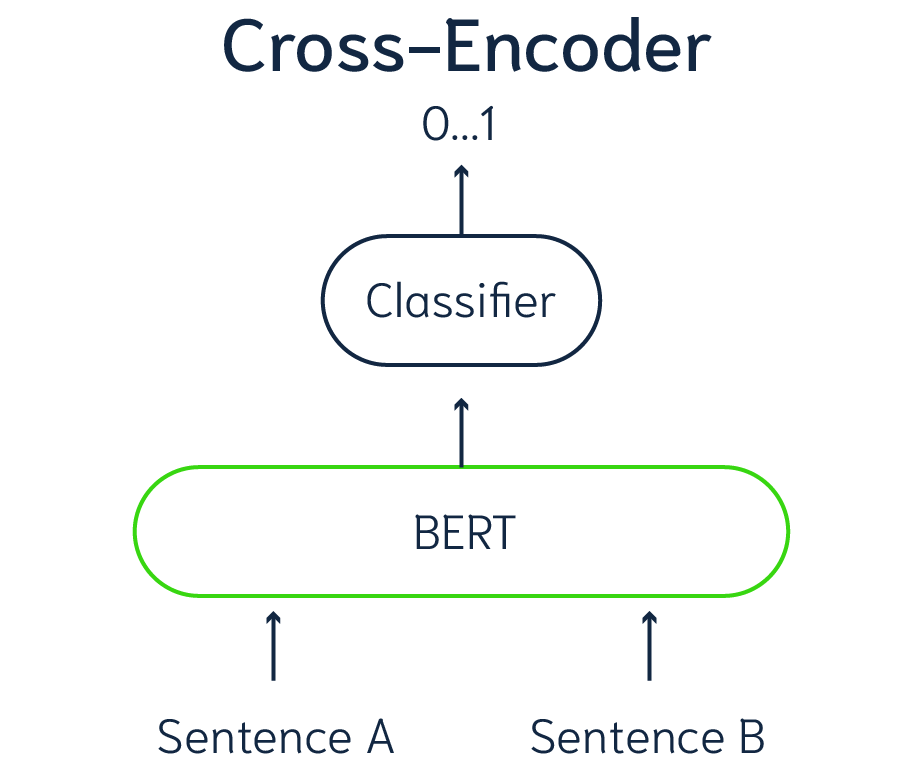
\includegraphics[width=0.5\textwidth]{Images/cross-encoder.png} % Nhớ upload ảnh và đặt đúng tên file
    \vspace{0.7cm}
    \caption{Sơ đồ kiến trúc Cross-Encoder với đầu vào ghép đôi và đầu ra phân loại}
    \label{fig:cross_encoder_arch}
% ... (Phần code chèn ảnh ở trên giữ nguyên) ...
\end{figure}

% Thêm \noindent vào đây
\noindent Quan sát Hình \ref{fig:cross_encoder_arch}, ta có thể phân tích cơ chế hoạt động qua ba giai đoạn chính:

% Thêm \noindent vào đây và dùng \vspace để tạo khoảng cách nhỏ cho thoáng
\vspace{0.2cm} 
\noindent \textbf{1. Tầng Đầu vào (Input Layer):} \\
Khác với Bi-Encoder xử lý hai nhánh độc lập, hình vẽ cho thấy Sentence A (đại diện cho truy vấn $q$) và Sentence B (đại diện cho văn bản ứng viên $d$) được đưa vào cùng một khối xử lý. Trong thực tế, hai chuỗi này được nối lại (concatenated) thành một chuỗi duy nhất, bắt đầu bằng token đặc biệt \texttt{[CLS]} và ngăn cách bởi \texttt{[SEP]}:
\begin{equation}
    Input = \texttt{[CLS]} \oplus q \oplus \texttt{[SEP]} \oplus d \oplus \texttt{[SEP]}
\end{equation}
\noindent \textbf{2. Khối xử lý trung tâm (BERT):} \\
Khối ``BERT'' trong sơ đồ đại diện cho các lớp Encoder của Transformer. Tại đây diễn ra cơ chế \textbf{Full Self-Attention} (tương tác sớm). Mỗi token trong Sentence A được phép nhìn thấy và tính toán trọng số chú ý với toàn bộ token trong Sentence B ngay từ những lớp đầu tiên. Điều này giúp mô hình nắm bắt được các sắc thái ngữ nghĩa phức tạp mà phương pháp so sánh vector độc lập thường bỏ sót.

\vspace{0.2cm}
\noindent \textbf{3. Tầng Phân loại (Classifier Head):} \\
Đầu ra của khối BERT là một chuỗi các vector ngữ cảnh, nhưng Cross-Encoder chỉ sử dụng vector tại vị trí \texttt{[CLS]} ($h_{CLS}$) để làm đại diện cho cả cặp câu. Như minh họa ở phần trên cùng của hình vẽ, vector này được đưa qua khối \textbf{Classifier} (thường là một lớp tuyến tính Linear Layer). Cuối cùng, hàm kích hoạt sẽ chuyển đổi kết quả thành một điểm số thực trong khoảng \textbf{0...1}. Giá trị này chính là xác suất phù hợp $P(y=1|q, d)$, dùng để xếp hạng lại (Reranking).

\subsubsection{So sánh hiệu năng với Bi-Encoder}


Việc lựa chọn giữa Cross-Encoder và Bi-Encoder luôn đòi hỏi sự cân nhắc kỹ lưỡng về sự đánh đổi giữa độ chính xác và hiệu suất tính toán. Để làm rõ sự khác biệt về mặt cấu trúc dẫn đến sự đánh đổi này, hãy quan sát sơ đồ so sánh dưới đây:

\begin{figure}[H]
    \centering
    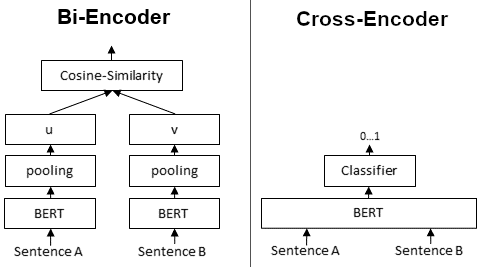
\includegraphics[width=0.8\textwidth]{Images/Bi_vs_Cross-Encoder.png} % Đảm bảo tên file ảnh đúng
    \vspace{0.5cm}
    \caption{Sơ đồ so sánh kiến trúc giữa Bi-Encoder (trái) và Cross-Encoder (phải)}
    \label{fig:bi_vs_cross}
\end{figure}


\noindent Quan sát Hình \ref{fig:bi_vs_cross}, ta thấy sự đối lập rõ rệt trong luồng xử lý dữ liệu:

\vspace{0.2cm}
\noindent \textbf{1. Về mặt Độ chính xác (Accuracy):} \\
Mô hình \textbf{Cross-Encoder} (bên phải hình vẽ) thể hiện sự vượt trội. Nhờ kiến trúc hợp nhất, cả hai câu (Sentence A và B) được đưa vào cùng một khối BERT ngay từ đầu. Điều này cho phép cơ chế Full Self-Attention hoạt động trên toàn bộ cặp câu, nắm bắt được các phụ thuộc phi tuyến tính phức tạp (non-linear dependencies). Đầu ra đi qua lớp \textit{Classifier} để trả về điểm số xác suất chính xác từ $0 \dots 1$.

Ngược lại, \textbf{Bi-Encoder} (bên trái hình vẽ) bị giới hạn bởi cấu trúc song song. Hai luồng thông tin Sentence A và Sentence B đi qua hai tháp BERT riêng biệt để tạo ra vector $u$ và $v$. Sự tương tác chỉ xảy ra ở bước cuối cùng thông qua hàm \textit{Cosine-Similarity}. Do thiếu sự tương tác sớm, Bi-Encoder thường gặp khó khăn trong các trường hợp đòi hỏi thấu hiểu ngữ nghĩa sâu hoặc khi truy vấn và văn bản có ít từ khóa chung.

\vspace{0.2cm}
\noindent \textbf{2. Về mặt Hiệu suất tính toán (Computational Efficiency):} \\
Tuy nhiên, cấu trúc tách biệt của \textbf{Bi-Encoder} lại mang đến lợi thế to lớn về tốc độ. Vì vector $v$ (đại diện cho sản phẩm) không phụ thuộc vào vector $u$ (truy vấn), chúng có thể được tính toán trước (pre-computed) và lưu trữ. Khi có truy vấn mới, hệ thống chỉ cần tính vector $u$ một lần và thực hiện tìm kiếm tương đồng (Approximate Nearest Neighbor Search) với chi phí rất thấp.

Trong khi đó, \textbf{Cross-Encoder} không thể mở rộng cho tác vụ tìm kiếm quy mô lớn. Do phải ghép nối truy vấn mới với \textit{từng} văn bản trong cơ sở dữ liệu để đưa vào mạng Transformer đồ sộ, việc áp dụng trực tiếp là bất khả thi trong thời gian thực. Vì vậy, trong thực tế, Cross-Encoder chỉ được sử dụng tối ưu trong giai đoạn Reranking trên một tập ứng viên nhỏ (ví dụ: $50-100$ items) đã được lọc sơ bộ bởi Bi-Encoder.

% ==============================================================================
% MỤC 6.2: PHƯƠNG PHÁP ĐỀ XUẤT (Tiếp nối)
% ==============================================================================

\subsection{Phương pháp đề xuất và Kiến trúc hệ thống}

Dựa trên các phân tích về hạn chế của mô hình đơn lẻ, dự án đề xuất triển khai chiến lược \textbf{Truy xuất và Xếp hạng lại (Retrieve-and-Rerank)}. Chiến lược này tận dụng sức mạnh bổ trợ của hai phương pháp mã hóa văn bản khác nhau nhằm đạt được sự cân bằng tối ưu giữa khả năng mở rộng trên dữ liệu lớn và độ chính xác trong thấu hiểu ngữ nghĩa.

\subsubsection{Quy trình Truy xuất hai giai đoạn (Two-Stage Retrieval Pipeline)}

Để giải quyết bài toán gợi ý sản phẩm với độ chính xác cao trên không gian dữ liệu lớn, hệ thống được thiết kế theo quy trình truy xuất hai giai đoạn (Retrieve-and-Rerank), hoạt động như một bộ lọc phễu từ thô đến tinh. Để hình dung rõ luồng dữ liệu và sự thay đổi về kích thước tập ứng viên qua từng bước, hãy xem xét sơ đồ quy trình dưới đây:

\begin{figure}[H]
    \centering
    % Nhớ upload file ảnh pipeline_2stage.png vào Overleaf trước
    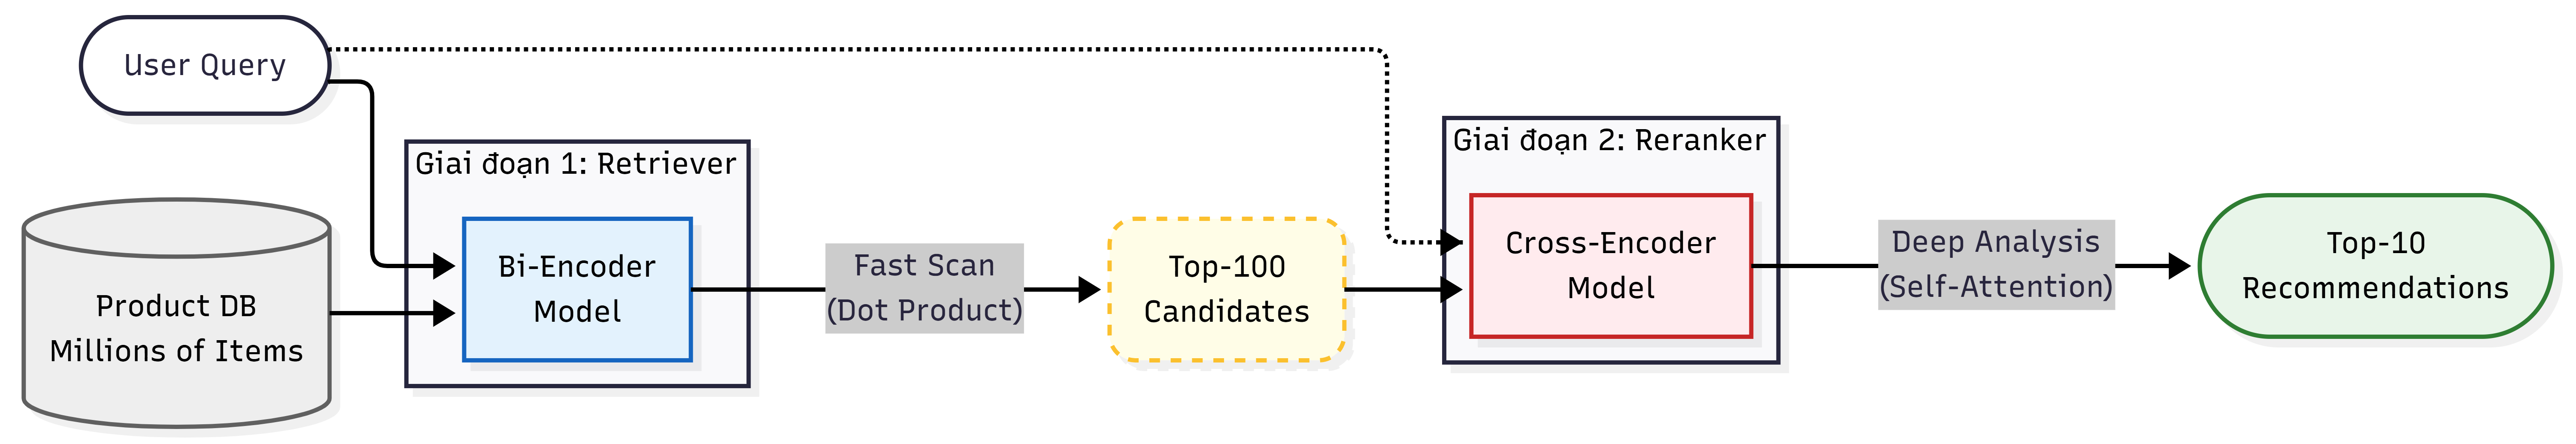
\includegraphics[width=1.0\textwidth]{Images/Two-Stage Product Retrieval-2025-12-21-060715.png}
    \vspace{0.5cm}
    \caption{Sơ đồ quy trình phễu lọc hai giai đoạn: Từ hàng triệu sản phẩm xuống Top 10}
    \label{fig:pipeline_2stage}
\end{figure}

\noindent Quan sát Hình \ref{fig:pipeline_2stage}, quy trình xử lý được chia thành hai pha riêng biệt với đặc thù trái ngược nhau về chi phí tính toán và độ chính xác:

\begin{enumerate}
    \item \textbf{Giai đoạn Sàng lọc thô (Retriever - Bi-Encoder):}
    Tại bước này (khối màu xanh dương), hệ thống quét nhanh qua toàn bộ cơ sở dữ liệu chứa hàng triệu sản phẩm. Mục tiêu là tốc độ. Đầu ra là tập hợp $K=100$ ứng viên tiềm năng nhất (khối màu vàng).
    
    \item \textbf{Giai đoạn Sàng lọc tinh (Reranker - Cross-Encoder):}
    Tập hợp 100 ứng viên được chuyển tiếp sang mô hình Cross-Encoder (khối màu đỏ). Tại đây, mô hình thực hiện phân tích ngữ cảnh sâu (Deep Analysis). Kết quả cuối cùng là Top 10 sản phẩm tối ưu nhất (khối màu xanh lá) được trả về cho người dùng.
\end{enumerate}

\noindent Trong dự án này, mô hình \texttt{cross-encoder/ms-marco-MiniLM-L6-v2} được lựa chọn làm mô hình cơ sở (base model) để tinh chỉnh (fine-tune) trên miền dữ liệu thương mại điện tử. Để mô hình có thể xử lý đồng thời thông tin người dùng và sản phẩm, dữ liệu đầu vào được cấu trúc lại thành một chuỗi token nối tiếp theo định dạng chuẩn của Transformer:
\begin{equation}
    \texttt{[CLS] Context [SEP] Candidate [SEP]}
\end{equation}
\noindent Trong cấu trúc trên, thành phần \textbf{Context} được xây dựng từ sự kết hợp giữa lịch sử tương tác và truy vấn hiện tại, giúp mô hình đối chiếu nhu cầu tìm kiếm với sở thích cá nhân. Ngay sau token ngăn cách là thành phần \textbf{Candidate}, bao gồm tiêu đề và mô tả sản phẩm, cung cấp ngữ cảnh chi tiết để mô hình đánh giá độ tương quan ngữ nghĩa.

\vspace{0.2cm} % Tạo khoảng cách nhỏ giữa Input và Output cho thoáng mắt

\noindent Quá trình tính toán kết quả cuối cùng được thực hiện tại lớp đầu ra của mạng nơ-ron. Cụ thể, vector đại diện tại vị trí \texttt{[CLS]} ($h_{CLS}$) được đưa qua một lớp tuyến tính (Linear Layer) để chiếu về một giá trị thực (logit). Giá trị này sau đó được chuyển đổi thành xác suất $P(y=1|\text{Context}, \text{Candidate})$, đại diện cho mức độ phù hợp dùng để xếp hạng sản phẩm.

% ... (Giữ nguyên phần mô tả Input/Output phía sau) ...


% ==============================================================================
% MỤC 6.2.2: LỰA CHỌN MÔ HÌNH CƠ SỞ
% ==============================================================================

\subsubsection{Lựa chọn Mô hình cơ sở: cross-encoder/ms-marco-MiniLM-L6-v2}

Để giải quyết bài toán mâu thuẫn giữa độ chính xác cao và thời gian phản hồi thấp trong hệ thống gợi ý thời gian thực, báo cáo này lựa chọn mô hình \path{cross-encoder/ms-marco-MiniLM-L6-v2}. Đây là một phiên bản mô hình ngôn ngữ được nén (compressed) từ kiến trúc BERT khổng lồ. Để hiểu rõ cơ sở khoa học của sự lựa chọn này, cần xem xét kỹ thuật nền tảng là Truyền tri thức (Knowledge Distillation) và kiến trúc đặc thù của MiniLM.

% ==============================================================================
% MỤC TỔNG QUAN VỀ KNOWLEDGE DISTILLATION (KD) - CHI TIẾT
% ==============================================================================

    % ==============================================================================
% MỤC 2.2.1 TỔNG QUAN KD (Giữ nguyên như bạn đã cung cấp)
% ==============================================================================
\paragraph{Tổng quan về Knowledge Distillation (KD)} \mbox{} \\

Trong những năm gần đây, sự bùng nổ của các Mô hình Ngôn ngữ Tiền huấn luyện (Pre-trained Language Models - PLMs) như BERT, RoBERTa hay XLNet đã tạo ra những bước đột phá trong xử lý ngôn ngữ tự nhiên. Tuy nhiên, đi kèm với hiệu suất cao là kích thước khổng lồ với hàng trăm triệu tham số. Điều này đặt ra rào cản lớn về tài nguyên tính toán và độ trễ (latency) khi triển khai trên các hệ thống thực tế hoặc thiết bị biên (edge devices).

Để giải quyết bài toán cân bằng giữa hiệu suất và tài nguyên, kỹ thuật \textbf{Truyền tri thức (Knowledge Distillation - KD)} được áp dụng như một giải pháp nén mô hình hiệu quả. Về bản chất, KD là quá trình chuyển giao khả năng khái quát hóa từ một mô hình lớn, phức tạp (Teacher) sang một mô hình nhỏ gọn hơn (Student) mà không làm giảm đáng kể độ chính xác.

Để hiểu rõ cơ chế hoạt động bên trong, hãy xem xét sơ đồ quy trình KD dưới đây:

\begin{figure}[H]
    \centering
    % Sử dụng tên file ảnh bạn đã upload
    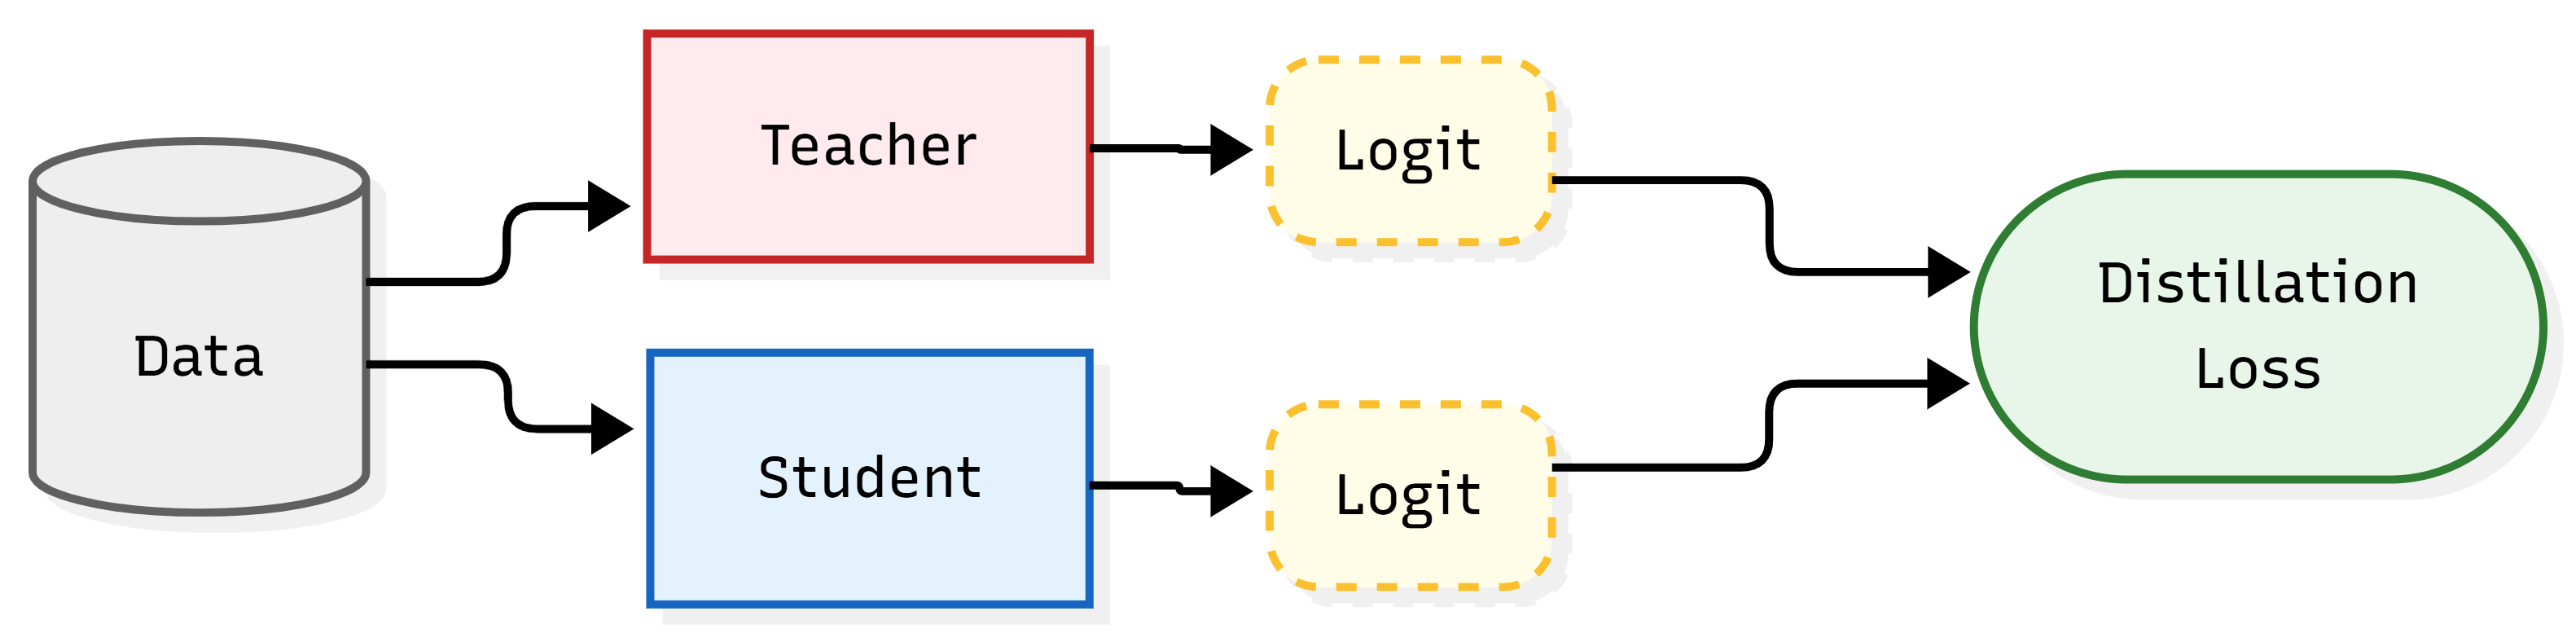
\includegraphics[width=0.9\textwidth]{Images/Untitled diagram-2025-12-21-064145.png}
    \vspace{0.5cm}
    \caption{Sơ đồ quy trình Knowledge Distillation: Mô hình Student học cách mô phỏng phân phối xác suất (Logits) của Teacher.}
    \label{fig:kd_process}
\end{figure}

\vspace{0.2cm}
\noindent Quan sát Hình \ref{fig:kd_process}, quy trình truyền tri thức bắt đầu bằng việc đưa dữ liệu đầu vào (khối \textbf{Data} màu xám) đồng thời vào hai luồng xử lý song song. Nhánh phía trên là mô hình \textbf{Teacher} (khối màu đỏ) với đặc điểm kích thước lớn và đã hội tụ, đóng vai trò nguồn tri thức chuẩn nên các trọng số thường được đóng băng để đảm bảo tính ổn định. Nhánh phía dưới là mô hình \textbf{Student} (khối màu xanh), đối tượng chính cần huấn luyện với kiến trúc được thiết kế nhỏ gọn hơn nhằm tối ưu hóa tài nguyên và tốc độ suy diễn.

\vspace{0.2cm}
\noindent Điểm cốt lõi của phương pháp này nằm ở việc khai thác thông tin từ các khối \textbf{Logit} (màu vàng). Thay vì chỉ dựa vào nhãn cứng (Hard Labels) vốn chỉ cung cấp đáp án đúng sai tuyệt đối, mô hình Student học từ phân phối xác suất đầu ra của Teacher. Các giá trị Logit này chứa đựng \textbf{Tri thức tiềm ẩn (Latent Knowledge)}—những thông tin ẩn về mối quan hệ ngữ nghĩa giữa các lớp mà nhãn cứng không thể thể hiện. Ví dụ, thông qua Logit, Teacher có thể chỉ ra rằng một đối tượng ``con chó'' có nét tương đồng về mặt đặc trưng với ``con mèo'' nhiều hơn là ``xe hơi''. Việc nắm bắt được các sắc thái tinh tế này giúp Student hình thành tư duy tổng quát hóa tốt hơn thay vì chỉ học thuộc lòng đáp án.

\vspace{0.2cm}
\noindent Cuối cùng, kết quả dự đoán của hai mô hình được đưa vào khối \textbf{Distillation Loss} (màu xanh lá) để so khớp. Đây là thành phần quan trọng nhất dùng để định hướng quá trình học, có nhiệm vụ đo lường khoảng cách giữa phân phối xác suất của Teacher và Student. Mục tiêu của quá trình huấn luyện là cực tiểu hóa sự khác biệt này, ép buộc Student phải mô phỏng lại ``cách tư duy'' của Teacher. Trong thực tế, hàm mất mát tổng thể thường là sự kết hợp có trọng số giữa hàm mất mát chưng cất (học theo Teacher) và hàm mất mát của tác vụ chính (học theo nhãn thực tế), giúp cân bằng giữa khả năng bắt chước và độ chính xác trên tập dữ liệu.

% ==============================================================================
% MỤC 2.2.2 PHÂN TÍCH MINILM (Đã chỉnh sửa phần dẫn nhập)
% ==============================================================================

% ==============================================================================
% MỤC 2.2.2 PHÂN TÍCH MINILM & LÝ DO LỰA CHỌN (ĐÃ HỢP NHẤT)
% ==============================================================================

\paragraph{Phân tích chuyên sâu về MiniLM và Ứng dụng trong Dự án} \mbox{} \\

Mặc dù phương pháp Knowledge Distillation truyền thống đã chứng minh được hiệu quả, nhưng việc áp dụng trực tiếp vào các mô hình Transformer phức tạp vẫn gặp nhiều hạn chế, đặc biệt là sự ràng buộc về kích thước chiều ẩn (Hidden Dimension) giữa Teacher và Student. Để khắc phục vấn đề này và tối ưu hóa sâu hơn vào cơ chế cốt lõi của Transformer, Wang \etal \cite{32} đã đề xuất kiến trúc \textbf{MiniLM} (Miniature Language Model). 

Khác với các phương pháp nén mô hình thông thường chỉ tập trung vào lớp đầu ra (Output Layer), MiniLM là phương pháp nén không phụ thuộc vào tác vụ (Task-Agnostic), đi sâu vào việc chưng cất thành phần quan trọng nhất tạo nên sức mạnh của Transformer: cơ chế \textbf{Self-Attention}.

\vspace{0.3cm}
\noindent \textit{1. Đặt vấn đề và Kiến thức cơ sở (Preliminary)}

Mạng Transformer được xây dựng dựa trên cơ chế Multi-Head Self-Attention. Trong một lớp Transformer, giả sử đầu vào là chuỗi vector $X$, Multi-Head Self-Attention bao gồm $H$ đầu chú ý. Tại mỗi đầu $h$, đầu vào được chiếu qua các ma trận trọng số $W_Q, W_K, W_V$ để tạo ra các vector Query ($Q_h$), Key ($K_h$) và Value ($V_h$). Công thức tính toán Standard Attention tại đầu $h$ được định nghĩa \cite{41}:

\begin{equation}
    \text{Attention}_h(Q, K, V) = \text{Softmax}\left(\frac{Q_h K_h^T}{\sqrt{d_k}}\right) V_h
\end{equation}
Trong đó $d_k$ là kích thước chiều của vector key.

\noindent \textbf{Giải thích các tham số:}
\begin{itemize}
    \item $Q_h, K_h, V_h$: Lần lượt là các ma trận Query (Truy vấn), Key (Khóa) và Value (Giá trị) tại đầu chú ý thứ $h$.
    \item $K_h^T$: Ma trận chuyển vị của $K_h$, dùng để tính tích vô hướng (độ tương đồng) với $Q_h$.
    \item $d_k$: Kích thước chiều (dimension size) của vector Key.
    \item $\sqrt{d_k}$: Hệ số tỷ lệ (scaling factor) giúp ổn định giá trị tích vô hướng trước khi đưa vào hàm Softmax.
\end{itemize}

\vspace{0.3cm}
\noindent \textit{2. Phương pháp Chưng cất Sự chú ý Sâu (Deep Self-Attention Distillation)}

MiniLM tập trung chuyển giao tri thức tại \textbf{lớp Transformer cuối cùng}, nơi chứa đựng những đặc trưng ngữ nghĩa tinh túy nhất. Quá trình này dựa trên hai thành phần cốt lõi được trình bày tại hình \ref{fig:minilm_arch}:
% --- CHÈN HÌNH ẢNH MINILM ---
\begin{figure}[H]
    \centering
    % Thay 'minilm_architecture.png' bằng tên file ảnh thực tế của bạn
    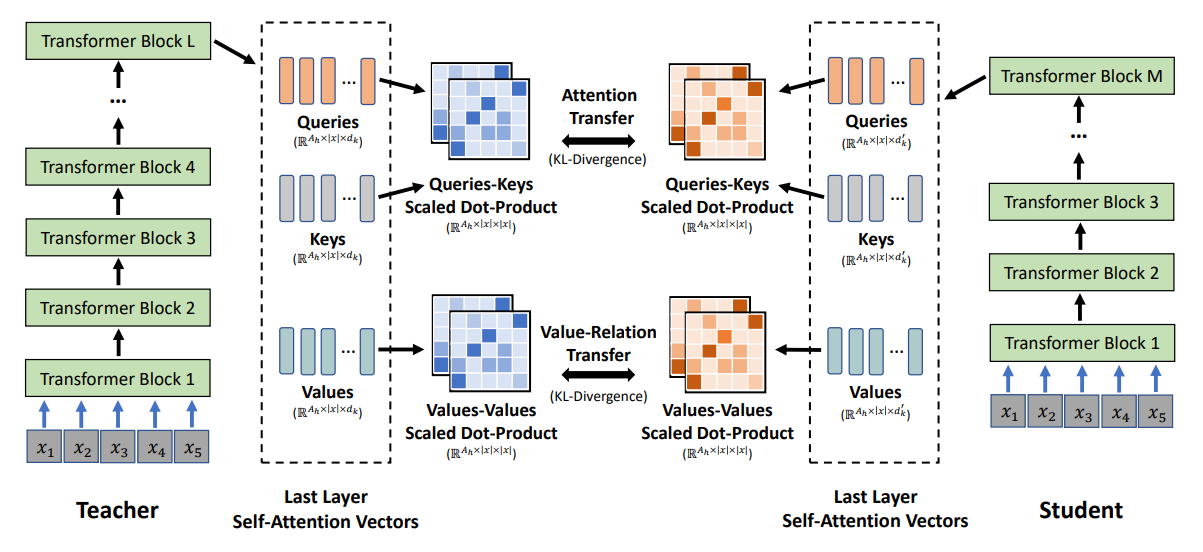
\includegraphics[width=0.9\textwidth]{Images/minilm_architecture.png} 
    \vspace{0.5cm}
    \caption{Tổng quan kiến trúc Deep Self-Attention Distillation của MiniLM.}
    \label{fig:minilm_arch}
\end{figure}


\vspace{0.2cm}

\noindent \textbf{Thành phần A: Phân phối Sự chú ý (Self-Attention Distributions).} \\
Ma trận chú ý $A_h$ biểu diễn mối quan hệ phụ thuộc giữa các từ, được tính như sau \cite{32}:

\begin{equation}
    A_h = \text{Softmax}\left(\frac{Q_h K_h^T}{\sqrt{d_k}}\right)
\end{equation}
Hàm mất mát Kullback-Leibler (KL-Divergence) được sử dụng để giảm thiểu sự khác biệt giữa Teacher ($T$) và Student ($S$):

\begin{equation}
    \mathcal{L}_{AT} = \frac{1}{H} \sum_{h=1}^{H} D_{KL}(A_h^T || A_h^S)
\end{equation}

\vspace{0.2cm}

\noindent \textbf{Thành phần B: Quan hệ Giá trị (Self-Attention Value Relations).} \\
Đây là đóng góp đột phá của MiniLM, sử dụng quan hệ giữa các vector Value ($V-V$) thay vì $Q-K$:

\begin{equation}
    VR_h = \text{Softmax}\left(\frac{V_h V_h^T}{\sqrt{d_k}}\right)
\end{equation}

Hàm mất mát tương ứng cho thành phần này là \cite{32}:


\begin{equation}
    \mathcal{L}_{VR} = \frac{1}{H} \sum_{h=1}^{H} D_{KL}(VR_h^T || VR_h^S)
\end{equation}

\noindent \textbf{Giải thích ký hiệu:}
\begin{itemize}
    \item $A_h^T, A_h^S$: Phân phối chú ý của mô hình Teacher và Student.
    \item $VR_h^T, VR_h^S$: Quan hệ giá trị của mô hình Teacher và Student.
    \item $D_{KL}$: Độ phân kỳ Kullback-Leibler, đo lường sự khác biệt giữa hai phân phối xác suất.
    \item $H$: Tổng số lượng đầu chú ý (Attention Heads).
\end{itemize}

\vspace{0.3cm}
\noindent \textit{3. Cơ sở lựa chọn phiên bản MiniLM-L6-v2 cho dự án}

\noindent Từ nền tảng lý thuyết vững chắc về cơ chế truyền tri thức kép nêu trên, phiên bản cụ thể \texttt{MiniLM-L6-v2} đã được lựa chọn để triển khai module Reranking cho hệ thống. Quyết định này dựa trên sự cân bằng tối ưu giữa hiệu quả kiến trúc, tốc độ và chất lượng. Cụ thể, với cấu hình thu nhỏ gồm 6 lớp (L6) và chiều ẩn 384, mô hình đã loại bỏ hoàn toàn sự dư thừa tham số thường thấy ở các kiến trúc lớn như BERT-Base, trong khi vẫn duy trì được khả năng suy luận ngữ nghĩa phức tạp nhờ thừa hưởng trọn vẹn Quan hệ Giá trị từ Teacher. Hơn nữa, kết quả thực nghiệm chứng minh \texttt{MiniLM-L6-v2} đạt tốc độ suy diễn (Inference) nhanh hơn gấp 2 lần so với BERT-Base. Đây là yếu tố tiên quyết đối với bài toán Reranking, giúp giữ độ trễ hệ thống ở mức thấp nhất (low latency) để đảm bảo trải nghiệm người dùng. Mặc dù kích thước giảm đi đáng kể, mô hình vẫn bảo toàn được hơn 90\% độ chính xác so với mô hình gốc trên các bảng xếp hạng chuẩn (Benchmarks), qua đó đảm bảo danh sách gợi ý cuối cùng luôn đạt độ tương quan cao nhất.


% ==============================================================================
% MỤC 6.2.2.2: ĐẶC TẢ MÔ HÌNH VÀ DỮ LIỆU
% ==============================================================================

\paragraph{Bộ dữ liệu Tiền huấn luyện: MS MARCO (Passage Ranking)} \mbox{} \\

Mô hình \texttt{cross-encoder/ms-marco-MiniLM-L6-v2} được lựa chọn làm cơ sở cho dự án nhờ vào quá trình tiền huấn luyện (pre-training) bài bản trên bộ dữ liệu \textbf{MS MARCO} (Microsoft Machine Reading Comprehension). Theo công bố khoa học của Nguyen \etal \cite{42}, đây là nền tảng quan trọng giúp mô hình học được các đặc trưng ngôn ngữ tự nhiên và logic xếp hạng thông tin từ quy mô dữ liệu lớn trước khi được tinh chỉnh cho các tác vụ cụ thể.

Điểm làm nên hiệu suất vượt trội của phiên bản mô hình này nằm ở chiến lược dữ liệu được cộng đồng \textit{Sentence-Transformers} áp dụng. Cụ thể, trong quá trình phát triển mô hình gốc, thay vì sử dụng dữ liệu thô ban đầu từ Microsoft, các tác giả đã lựa chọn phiên bản tối ưu hóa có tích hợp kỹ thuật \textbf{Hard Negatives mining}

% \footnote{\url{https://huggingface.co/datasets/sentence-transformers/msmarco-hard-negatives}}
. Kỹ thuật này tạo ra các bộ ba (Triplets) bao gồm Truy vấn, Mẫu dương và Mẫu âm, thay vì ghép cặp ngẫu nhiên. Về mặt quy mô, tập dữ liệu này bao gồm hơn 1.000.000 truy vấn thực tế từ Bing và hơn 8.800.000 đoạn văn bản, tất cả đều được gán nhãn thủ công với độ tin cậy cao.

Chính cấu trúc dữ liệu dạng Triplet này đã định hình khả năng hiểu ngữ nghĩa của mô hình trước khi được đưa vào áp dụng trong dự án. Bảng \ref{tab:msmarco_example} dưới đây minh họa mẫu dữ liệu mà mô hình đã được học, trong đó Hard Negative tuy chứa nhiều từ khóa trùng khớp (lexical overlap) nhưng sai lệch hoàn toàn về ngữ nghĩa hoặc đối tượng.


\begin{table}[H]
    \centering
    \renewcommand{\arraystretch}{1.3}
    
    \begin{tabular}{|p{0.15\textwidth}|p{0.5\textwidth}|p{0.25\textwidth}|}
        \hline
        \textbf{Thành phần} & \textbf{Nội dung văn bản} & \textbf{Phân tích ngữ nghĩa} \\
        \hline
        \textbf{Query} & \textit{``symptoms of heat exhaustion''} (Triệu chứng kiệt sức do nhiệt) & Truy vấn tìm kiếm thông tin y tế cho người. \\
        \hline
        \textbf{Positive} & \textit{``Symptoms of heat exhaustion include heavy sweating, rapid pulse...''} & Đoạn văn chứa câu trả lời chính xác, khớp ý định. \\
        \hline
        \textbf{Negative} & \textit{``Heat exhaustion is a condition whose symptoms... in dogs.''} & \textbf{Hard Negative:} Rất giống query nhưng nói về chó (dogs) thay vì người. \\
        \hline
    \end{tabular}
    \caption{Ví dụ mẫu dữ liệu Triplet trong MS MARCO với Hard Negative}
    \label{tab:msmarco_example}
\end{table}

\noindent Việc lựa chọn MS MARCO làm tiêu chuẩn vàng (Gold Standard) cho tác vụ này xuất phát từ ba đặc điểm ưu việt. Đầu tiên là tính chất thực tế (Real-world Distribution), nơi các truy vấn phản ánh đúng ngôn ngữ tự nhiên của người dùng bao gồm cả từ lóng hay lỗi chính tả, giúp mô hình bền vững hơn khi triển khai thực tế. Thứ hai là sự đa dạng về chủ đề (Topic Diversity) bao phủ từ y tế, công nghệ đến đời sống, giúp mô hình có khả năng khái quát hóa tốt. Cuối cùng và quan trọng nhất là khả năng chuyển giao (Transferability); nhờ lượng tri thức nền khổng lồ này, mô hình có thể dễ dàng thích nghi và tinh chỉnh (fine-tune) hiệu quả khi chuyển sang miền dữ liệu thương mại điện tử của Amazon.

% MỤC 6.2.2.3: ĐẶC TẢ MÔ HÌNH CROSS-ENCODER (Đưa xuống sau)
% ==============================================================================
\paragraph{Đặc tả Mô hình Cross-Encoder: cross-encoder/ms-marco-MiniLM-L6-v2} \mbox{} \\

Sau khi xác lập kiến trúc nền tảng là MiniLM và bộ dữ liệu nguồn là MS MARCO, dự án lựa chọn phiên bản cụ thể \texttt{cross-encoder/ms-marco-MiniLM-L6-v2}\footnote{Link mô hình: \url{https://huggingface.co/cross-encoder/ms-marco-MiniLM-L6-v2}} làm điểm khởi đầu (checkpoint) cho quá trình huấn luyện. Đây không phải là một mô hình được khởi tạo ngẫu nhiên, mà là kết quả của một \textbf{quy trình huấn luyện kế thừa (Multi-stage Training Pipeline)} được thực hiện bài bản qua nhiều giai đoạn.

\vspace{0.2cm}
\noindent \textbf{1. Nguồn gốc và Quy trình hình thành} \\
Quá trình phát triển mô hình (hình \ref{fig:model_creation}) bắt đầu từ kiến trúc \textit{MiniLM gốc} của Microsoft, được nén từ BERT để học các biểu diễn ngôn ngữ chung (General Language Understanding). Ở giai đoạn thích nghi (Adaptation), mô hình được chuyển đổi sang định dạng tương thích với thư viện \textit{Sentence-Transformers} (phiên bản \texttt{nreimers/MiniLM-L6-H384-uncased}). Tuy nhiên, bước ngoặt quyết định nằm ở giai đoạn tinh chỉnh (Fine-tuning), nơi mô hình được huấn luyện chuyên sâu trên tập dữ liệu \textbf{MS MARCO Passage Ranking}. Mục tiêu của giai đoạn này là trang bị cho mô hình kỹ năng xếp hạng và phân biệt đoạn văn phù hợp với câu hỏi, chuyển hóa từ một mô hình ngôn ngữ chung thành một Cross-Encoder chuyên dụng. Cuối cùng, để tối ưu hóa cho môi trường thực tế, các trọng số đã được Quantized nhằm giảm kích thước và tăng tốc độ suy diễn.

\begin{figure}[H]
    \centering
    % Đảm bảo đường dẫn ảnh đúng với thư mục trong Overleaf của bạn
    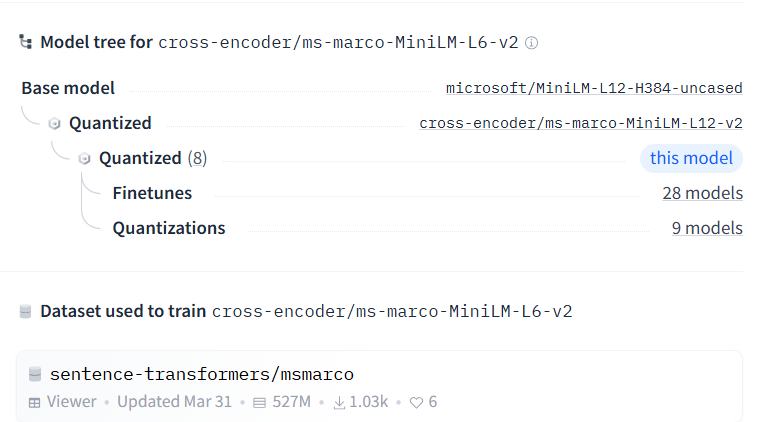
\includegraphics[width=0.9\textwidth]{Images/model_lineage.png}
    \vspace{1cm}
    \caption{Quy trình phát triển mô hình: Từ kiến trúc MiniLM gốc, qua bước tinh chỉnh (Fine-tuning) trên dữ liệu MS MARCO để tạo thành Cross-Encoder hoàn chỉnh.}
    \label{fig:model_creation}
\end{figure}

\noindent \textbf{2. Thông số kỹ thuật và Kiến trúc mạng} \\
Về mặt đặc tả kỹ thuật, mô hình sở hữu cấu trúc gọn nhẹ với \textbf{6 lớp Transformer (Layers)}, chiều ẩn (Hidden size) 384 và 12 Attention Head, tổng hợp thành khoảng \textbf{22.7 triệu tham số}. Khác với các mô hình BERT tiêu chuẩn (thường có hơn 110 triệu tham số), kích thước này cho phép triển khai hiệu quả trên các hệ thống có tài nguyên hạn chế.

Dữ liệu đầu vào của mô hình được xử lý theo cơ chế nối tiếp cặp văn bản: \texttt{[CLS] Query [SEP] Passage [SEP]}, với tổng độ dài tối đa cho phép là \textbf{512 tokens}. Tại đầu ra, một lớp tuyến tính (Linear Layer) được gắn trực tiếp trên token \texttt{[CLS]} để thực hiện nhiệm vụ hồi quy, dự đoán điểm số logit $s \in (-\infty, +\infty)$ biểu thị mức độ phù hợp ngữ nghĩa giữa truy vấn và văn bản.

% ==============================================================================
% MỤC 6.3.1: CHUẨN BỊ DỮ LIỆU HUẤN LUYỆN
% ==============================================================================

% ==============================================================================
% MỤC 6.3: CHIẾN LƯỢC TINH CHỈNH (FINE-TUNING STRATEGY)
% ==============================================================================

\subsubsection{Chiến lược Tinh chỉnh mô hình (Fine-tuning Strategy)}

Mặc dù mô hình nền tảng \texttt{cross-encoder/ms-marco-MiniLM-L6-v2} đã sở hữu năng lực xếp hạng văn bản ấn tượng nhờ quá trình tiền huấn luyện trên dữ liệu MS MARCO, việc áp dụng trực tiếp mô hình này vào bài toán thương mại điện tử gặp phải thách thức lớn về sự \textbf{sai lệch miền dữ liệu (Domain Shift)}.

Dữ liệu MS MARCO chủ yếu là các câu hỏi tìm kiếm thông tin chung (General Web Search), trong khi truy vấn trên Amazon mang tính chất giao dịch (Transactional Queries), chứa đựng nhiều mã định danh sản phẩm (ASIN), tên thương hiệu cụ thể và các từ khóa đặc thù ngành hàng (như ``OLED'', ``noise-cancelling''). Hơn nữa, hành vi tìm kiếm của người dùng thương mại điện tử đòi hỏi độ chính xác cực cao.

Do đó, dự án đề xuất chiến lược tinh chỉnh (Fine-tuning) dựa trên nguyên lý \textbf{Chuyển giao tri thức (Transfer Learning)}. Mục tiêu là chuyển đổi một mô hình xếp hạng văn bản phổ thông thành một chuyên gia xếp hạng sản phẩm. Quá trình này được thực hiện thông qua việc huấn luyện giám sát trên hai nguồn dữ liệu bổ trợ nhau: dữ liệu hành vi thực tế (ESCI) và dữ liệu tổng hợp từ AI \cite{34}.

% ------------------------------------------------------------------------------
% MỤC 6.3.1: CHUẨN BỊ DỮ LIỆU
% ------------------------------------------------------------------------------

\paragraph{Chuẩn bị dữ liệu huấn luyện} \mbox{} \\

Chất lượng của mô hình Cross-Encoder phụ thuộc tiên quyết vào chất lượng của các cặp dữ liệu \texttt{(Query, Product, Label)}. Để đạt được sự cân bằng giữa độ chính xác từ khóa và khả năng thấu hiểu ngôn ngữ tự nhiên, hệ thống dữ liệu huấn luyện được xây dựng từ hai nguồn chính.
\vspace{0.5cm}

% ==============================================================================
% MỤC 1: BỘ DỮ LIỆU ESCI
% ==============================================================================

\noindent \textbf{1. Bộ dữ liệu ESCI (Amazon Shopping Queries)} \\
Nguồn dữ liệu cốt lõi được sử dụng để tinh chỉnh mô hình là bộ dữ liệu \textbf{ESCI (Shopping Queries Dataset)}. Đây là tập dữ liệu quy mô lớn được công bố bởi nhóm nghiên cứu Amazon Science, được cộng đồng học thuật công nhận là tiêu chuẩn vàng để đánh giá các thuật toán tìm kiếm sản phẩm \cite{33}.

Điểm đặc biệt của bộ dữ liệu này nằm ở hệ thống nhãn đa cấp độ, được viết tắt là \textbf{ESCI}, mô tả chính xác sắc thái ngữ nghĩa giữa truy vấn của người dùng và sản phẩm trả về. Cụ thể, bốn mức độ tương quan được định nghĩa như sau:

\begin{itemize}
    \item \textbf{Exact (E - Khớp hoàn toàn):} Sản phẩm đáp ứng chính xác nhu cầu của người dùng về mọi mặt như chức năng, thương hiệu và thông số kỹ thuật (Ví dụ: Tìm ``iPhone 12'' và kết quả là điện thoại iPhone 12).
    \item \textbf{Substitute (S - Thay thế):} Sản phẩm có chức năng tương đương nhưng khác biệt về một số đặc tính quan trọng như thương hiệu, màu sắc hoặc mẫu mã, mà người dùng có thể cân nhắc nếu sản phẩm chính hết hàng (Ví dụ: Tìm ``giày chạy bộ Nike'' nhưng kết quả là ``giày Adidas'').
    \item \textbf{Complement (C - Bổ trợ):} Sản phẩm không thỏa mãn trực tiếp truy vấn nhưng thường được mua kèm hoặc hỗ trợ cho sản phẩm chính (Ví dụ: Tìm ``iPhone 12'' nhưng kết quả là ``Ốp lưng'' hoặc ``Dây sạc'').
    \item \textbf{Irrelevant (I - Không liên quan):} Sản phẩm hoàn toàn không liên quan đến truy vấn.
\end{itemize}

\begin{table}[H]
    \centering
    \caption{Ví dụ minh họa và chiến lược gán nhãn nhị phân cho ESCI}
    
    \small 
    \renewcommand{\arraystretch}{1.3} % Tăng khoảng cách dòng cho thoáng
    % Tổng độ rộng các cột: 0.18 + 0.32 + 0.12 + 0.28 = 0.90\textwidth (Vừa vặn)
    \begin{tabular}{|p{0.18\textwidth}|p{0.32\textwidth}|p{0.12\textwidth}|p{0.28\textwidth}|}
        \hline
        \centering \textbf{Truy vấn} & \centering \textbf{Sản phẩm} & \centering \textbf{Nhãn gốc} & \textbf{Chiến lược Cross-Encoder} \\
        \hline
        iphone 12 case & OtterBox Commuter Case for iPhone 12 & \textbf{Exact} & \textbf{Positive (1):} Khớp hoàn toàn ý định. \\
        \hline
        iphone 12 case & iPhone 12 64GB Black (Unlocked) & \textbf{Irrelevant} & \textbf{Negative (0):} Sai loại sản phẩm. \\
        \hline
        nike running shoes & Adidas Ultraboost 21 Men's Shoe & \textbf{Substitute} & \textbf{Hard Negative (0):} Sai thương hiệu dù cùng chức năng. \\
        \hline
        camera canon & SD Card 64GB & \textbf{Complement} & \textbf{Hard Negative (0):} Sản phẩm đi kèm, không phải sản phẩm chính. \\
        \hline
    \end{tabular}
    \caption{Ví dụ minh họa và chiến lược gán nhãn nhị phân cho ESCI}
    \label{tab:esci_examples}
\end{table}

\noindent Vì Cross-Encoder trong dự án được thiết kế cho bài toán phân loại nhị phân (Binary Classification), hệ thống nhãn ESCI cần được quy hoạch lại một cách chiến lược. Theo đó, chỉ duy nhất nhãn \textbf{Exact} được coi là mẫu Dương (Label = 1). Tất cả các nhãn còn lại bao gồm Substitute, Complement và Irrelevant đều được gán là mẫu Âm (Label = 0). 

Chiến lược gán nhãn này đóng vai trò quan trọng trong việc tạo ra \textbf{(Hard Negatives)}. Đặc biệt, việc ép nhãn Substitute và Complement về 0 giúp mô hình học được sự phân biệt tinh tế: dù ``Adidas'' và ``Nike'' có sự tương đồng lớn về ngữ nghĩa vector (cùng là giày thể thao), nhưng trong ngữ cảnh tìm kiếm cụ thể, sự sai lệch về thương hiệu là không thể chấp nhận. Điều này giúp Cross-Encoder nắm bắt chặt chẽ các thực thể thương mại và ý định người dùng tốt hơn so với các phương pháp so khớp từ khóa thông thường.

\vspace{0.5cm} % Tạo khoảng cách giữa 2 mục

% --- 6.3.1.2 BLAIR DATASET ---

% --- 6.3.1.2 BLAIR DATASET ---

\noindent \textbf{2. Bộ dữ liệu Tổng hợp từ AI (Phương pháp BLAIR)} \\
Một hạn chế lớn của bộ dữ liệu ESCI là các truy vấn thường ngắn, thiên về từ khóa và thiếu cấu trúc ngữ pháp hoàn chỉnh. Trong khi đó, xu hướng người dùng thực tế ngày càng sử dụng các câu hỏi dài, mô tả nhu cầu phức tạp hoặc tìm kiếm bằng ngôn ngữ tự nhiên. Để lấp đầy khoảng trống này, phương pháp tạo dữ liệu tổng hợp dựa trên kỹ thuật \textbf{BLAIR} (Bridging Language and Items for Retrieval) được áp dụng để sinh ra các mẫu huấn luyện giàu ngữ nghĩa của Hou \etal \cite{34}.

\textbf{Quy trình sinh dữ liệu (Reverse Engineering):} \\
Để giải quyết vấn đề khan hiếm dữ liệu truy vấn phức tạp, quy trình Kỹ thuật đảo ngược được thực hiện bằng cách sử dụng Mô hình Ngôn ngữ Lớn (LLM) như GPT-4 hoặc Gemini. Quy trình này dựa trên giả định rằng nội dung đánh giá chi tiết chính là sự phản ánh nhu cầu tìm kiếm của người dùng nhưng ở thì quá khứ.

Các bước thực hiện cụ thể như sau:
\begin{enumerate}
    \item \textbf{Lựa chọn nguồn dữ liệu:} Các bài đánh giá từ tập dữ liệu Amazon Reviews 2023 được chọn làm đầu vào. Để đảm bảo chất lượng, dữ liệu được lọc theo tiêu chuẩn nghiêm ngặt: chỉ chọn các đánh giá \textbf{5 sao} (thể hiện sự hài lòng tuyệt đối với sản phẩm) và có độ dài tối thiểu \textbf{100 ký tự} (đảm bảo cung cấp đủ ngữ cảnh và thông tin chi tiết).
    \item \textbf{Prompting (Tạo câu lệnh):} LLM được yêu cầu đóng vai một người mua hàng tiềm năng, đọc nội dung review và viết lại thành một câu truy vấn tìm kiếm (Search Query) dưới góc nhìn thứ nhất, sao cho sản phẩm đó là câu trả lời phù hợp nhất.
    \item \textbf{Kết quả đầu ra:} Tạo thành các cặp dữ liệu \texttt{(Synthetic Query, Product)} với nhãn là Positive (1).
\end{enumerate}

\begin{table}[H]
    \centering
    
    \label{tab:blair_examples}
    \small
    \begin{tabular}{|p{0.35\textwidth}|p{0.35\textwidth}|p{0.2\textwidth}|}
        \hline
        \textbf{Review Gốc (Input)} & \textbf{Synthetic Query (Output bởi AI)} & \textbf{Sản phẩm} \\
        \hline
        ``Tôi thường xuyên phải bay đường dài và chiếc tai nghe này thực sự cứu cánh. Chức năng chống ồn chặn hoàn toàn tiếng động cơ máy bay. Pin dùng liên tục 30 tiếng vẫn chưa hết...'' & ``Tôi cần tìm một chiếc tai nghe chụp tai có khả năng chống ồn chủ động tốt nhất để đi máy bay và làm việc tập trung, yêu cầu thời lượng pin trâu.'' & Sony Headphones \\
        \hline
        ``Giày rất êm, phần đệm lót hỗ trợ cực tốt cho người bị bàn chân bẹt như tôi. Tôi đã chạy marathon mà không hề bị đau gan bàn chân.'' & ``Giày chạy bộ chuyên dụng tốt nhất giúp giảm đau và hỗ trợ chỉnh hình cho người có vòm bàn chân thấp hoặc bàn chân bẹt.'' & Adidas Shoes\\
        \hline
    \end{tabular}
    \caption{Ví dụ minh họa quy trình sinh dữ liệu tổng hợp từ Review}
\end{table}

\textbf{Tác dụng của bộ dữ liệu:} \\
Phương pháp này giúp tạo ra hàng nghìn cặp dữ liệu huấn luyện chất lượng cao. Các truy vấn tổng hợp này mang ngữ nghĩa phong phú hơn rất nhiều so với từ khóa đơn thuần, giúp mô hình Cross-Encoder học được cách xử lý các câu hỏi dài, nắm bắt được nhu cầu ẩn (latent needs) và ngữ cảnh sử dụng cụ thể của người dùng.

% ==============================================================================
% MỤC 6.3.2: KỸ THUẬT KHAI THÁC MẪU ÂM (HARD NEGATIVE MINING)
% ==============================================================================

\paragraph{Kỹ thuật khai thác mẫu âm (Hard Negative Mining)} \mbox{} \\

Trong bài toán xếp hạng và truy vấn thông tin, việc lựa chọn dữ liệu huấn luyện đóng vai trò quyết định đến độ chính xác của mô hình. Trong khi các mẫu dương (Positive samples) thường được xác định rõ ràng dựa trên nhãn dữ liệu (ví dụ: sản phẩm người dùng đã mua hoặc đánh giá 5 sao), việc lựa chọn mẫu âm (Negative samples) lại phức tạp hơn nhiều. Dự án áp dụng kỹ thuật \textbf{Khai thác mẫu âm khó (Hard Negative Mining)} để tối ưu hóa quá trình huấn luyện Cross-Encoder.

\vspace{0.3cm}
\noindent \textbf{Cơ sở lý thuyết và Sự cần thiết} \\
Thông thường, các phương pháp huấn luyện cơ bản sử dụng \textit{Mẫu âm ngẫu nhiên (Random Negatives)} -- tức là ghép một truy vấn bất kỳ với một sản phẩm được chọn ngẫu nhiên từ kho hàng. Tuy nhiên, phương pháp này bộc lộ hạn chế lớn khi áp dụng cho Cross-Encoder:
\begin{itemize}
    \item \textbf{Vấn đề hội tụ chậm (Inefficient Learning):} Trong không gian vector khổng lồ của hàng triệu sản phẩm, đại đa số các sản phẩm ngẫu nhiên là Dễ phân biệt (Easy Negatives). Ví dụ, với truy vấn \textit{``Laptop gaming''}, một mẫu âm ngẫu nhiên như \textit{``Nồi cơm điện''} hoàn toàn khác biệt về mặt ngữ nghĩa. Mô hình sẽ rất nhanh chóng đẩy xác suất của cặp này về 0, dẫn đến giá trị hàm mất mát (Loss) xấp xỉ 0 và triệt tiêu đạo hàm (vanishing gradients). Kết quả là mô hình ngừng học hỏi dù chưa thực sự hiểu sâu về đặc điểm sản phẩm.
    \item \textbf{Nhu cầu về khả năng phân biệt tinh tế:} Các nghiên cứu về Truy vấn thông tin mật độ cao (Dense Retrieval) của Karpukhin \etal \cite{35} đã chỉ ra rằng hiệu suất xếp hạng được cải thiện đáng kể khi mô hình được tiếp xúc với các mẫu nằm sát đường ranh giới quyết định (Decision Boundary). Đây là những mẫu sai nhưng nhìn có vẻ đúng.
\end{itemize}
Do đó, Hard Negative Mining là bắt buộc để ép Cross-Encoder phải học các đặc trưng chi tiết thay vì chỉ dựa vào các từ khóa bề mặt.

\vspace{0.3cm}
\noindent \textbf{Quy trình Khai thác mẫu khó} \\
Quy trình tạo mẫu âm khó được thực hiện trong giai đoạn tiền xử lý dữ liệu (Offline Pre-processing), tận dụng sức mạnh của mô hình Bi-Encoder để sàng lọc ứng viên. Các bước thực hiện cụ thể như sau:

\begin{enumerate}
    \item \textbf{Truy xuất ứng viên (Candidate Retrieval):} Sử dụng một mô hình Bi-Encoder (dạng kiến trúc Sentence-BERT gọn nhẹ) để mã hóa toàn bộ truy vấn trong tập huấn luyện và toàn bộ sản phẩm trong kho hàng thành các vector. Với mỗi truy vấn $q$, hệ thống thực hiện tìm kiếm Top-K (với $K=50$) sản phẩm có độ tương đồng vector cao nhất.
    \item \textbf{Lọc bỏ nhãn dương (Filtering Positives):} Trong danh sách 50 sản phẩm được Bi-Encoder gợi ý, hệ thống loại bỏ các sản phẩm trùng với nhãn dương (Ground Truth -- sản phẩm thực tế người dùng đã chọn) dựa trên ID sản phẩm.
    \item \textbf{Xác định Mẫu âm khó (Hard Negatives Identification):} Các sản phẩm còn lại trong Top-K chính là \textit{Hard Negatives}. Đặc điểm của chúng là có điểm tương đồng vector rất cao với truy vấn (do đó Bi-Encoder mới xếp vào top đầu), nhưng về mặt chức năng hoặc ý định người dùng thì chúng là kết quả sai. Các mẫu này thường chia sẻ nhiều từ khóa quan trọng với truy vấn hoặc thuộc cùng một danh mục sản phẩm, dễ gây nhầm lẫn cho các mô hình đơn giản.
\end{enumerate}

\vspace{0.3cm}
\noindent \textbf{Ví dụ minh họa thực tế} \\
Để làm rõ hiệu quả của phương pháp, hãy xem xét ví dụ với truy vấn \textbf{``iPhone 12''}:
\begin{itemize}
    \item \textbf{Random Negative:} \textit{``Giày Adidas''} $\rightarrow$ Quá dễ, Cross-Encoder không học được gì.
    \item \textbf{Hard Negative (Sinh ra từ Bi-Encoder):} \textit{``Ốp lưng iPhone 12 Pro Max''}.
\end{itemize}

Sản phẩm ốp lưng này chứa toàn bộ các từ khóa trong truy vấn (``iPhone'', ``12'') và vector ngữ nghĩa rất gần với điện thoại. Bi-Encoder thường không phân biệt tốt mối quan hệ giữa ``vật thể'' (điện thoại) và ``phụ kiện'' (ốp lưng). Khi đưa cặp \texttt{(``iPhone 12'', ``Ốp lưng iPhone 12 Pro Max'')} vào huấn luyện với nhãn 0, Cross-Encoder buộc phải chú ý đến từ khóa ``Ốp lưng'' (Case) để phạt nặng điểm số xuống thấp. Nhờ đó, mô hình học được sự phân biệt ngữ nghĩa sâu sắc mà Bi-Encoder đã bỏ sót.

\paragraph{Phương pháp huấn luyện} \mbox{} \\
% ==============================================================================
% MỤC 6.3.3: PHƯƠNG PHÁP HUẤN LUYỆN
% ==============================================================================

Để đảm bảo mô hình Cross-Encoder hội tụ ổn định và đạt hiệu suất tối ưu trên miền dữ liệu thương mại điện tử, quá trình huấn luyện được thiết lập dựa trên các kỹ thuật tiêu chuẩn của kiến trúc Transformer hiện đại. Các thành phần chính của quy trình huấn luyện bao gồm:

\vspace{0.3cm}
\noindent \textbf{Hàm mất mát (Loss Function):} \\
Dự án sử dụng hàm \textbf{Binary Cross-Entropy with Logits (BCEWithLogitsLoss)}. Vì bản chất của Cross-Encoder trong hệ thống này là giải quyết bài toán phân loại nhị phân (xác định một cặp \texttt{Query-Product} là Phù hợp hoặc Không phù hợp), mô hình sẽ xuất ra một giá trị thực (logits) thể hiện mức độ tương đồng. Hàm \texttt{BCEWithLogitsLoss} tích hợp lớp Sigmoid và hàm Cross-Entropy vào một bước tính toán duy nhất, giúp đảm bảo tính ổn định số học (numerical stability). Mục tiêu là tối thiểu hóa sai số giữa xác suất dự đoán và nhãn thực tế (1 cho Exact match và 0 cho các trường hợp còn lại).

\vspace{0.3cm}
\noindent \textbf{Trình tối ưu hóa (Optimizer):} \\
Chúng tôi lựa chọn \textbf{AdamW} (Adam with Weight Decay) làm thuật toán tối ưu hóa. Đây là tiêu chuẩn vàng cho việc huấn luyện các mô hình ngôn ngữ lớn như BERT hay RoBERTa. Khác với Adam truyền thống, AdamW tách biệt việc suy giảm trọng số (Weight Decay) khỏi việc tính toán gradient, giúp mô hình tổng quát hóa tốt hơn và hạn chế hiện tượng quá khớp (overfitting) trên tập dữ liệu huấn luyện.

\vspace{0.3cm}
\noindent \textbf{Cơ chế lập lịch tốc độ học (Learning Rate Scheduler):} \\
Việc huấn luyện Transformer rất nhạy cảm với tốc độ học. Nếu tốc độ học quá lớn ngay từ đầu, mô hình dễ bị mất ổn định (gradient explosion). Do đó, chiến lược \textbf{Linear Warmup} được áp dụng. Cụ thể, trong 10\% tổng số bước huấn luyện đầu tiên (warmup steps), tốc độ học sẽ tăng tuyến tính từ 0 lên mức tối đa (ví dụ $2e^{-5}$). Giai đoạn làm nóng này giúp các trọng số của mô hình di chuyển về vùng không gian tham số ổn định trước khi bắt đầu quá trình tối ưu hóa chính thức. Sau đó, tốc độ học giảm dần tuyến tính về 0 để giúp mô hình hội tụ tốt hơn.

\vspace{0.3cm}
\noindent \textbf{Chỉ số đánh giá (Evaluation Metrics):} \\
Do đặc thù của bài toán Reranking là sắp xếp thứ tự ưu tiên, việc sử dụng độ chính xác (Accuracy) đơn thuần là không phản ánh đúng trải nghiệm người dùng. Thay vào đó, hiệu năng mô hình được đo lường bằng các chỉ số xếp hạng chuyên dụng trên tập Validation:
\begin{itemize}
    \item \textbf{NDCG@10 (Normalized Discounted Cumulative Gain):} Đây là chỉ số quan trọng nhất, đo lường chất lượng xếp hạng có trọng số. NDCG đánh giá cao việc đưa các kết quả đúng lên các vị trí đầu tiên (top 1, top 2) hơn là các vị trí thấp hơn trong danh sách top 10.
    \item \textbf{MRR@10 (Mean Reciprocal Rank):} Đo lường nghịch đảo thứ hạng của kết quả đúng đầu tiên tìm được. Chỉ số này cho biết trung bình người dùng phải lướt xuống bao xa để thấy kết quả mong muốn đầu tiên.
\end{itemize}

\section{Kế hoạch thực hiện đề tài}
\begin{table}[H]
    \centering
    \caption{Kế hoạch thực hiện đề tài (15 Tuần)}
    \label{tab:project-timeline}
    \renewcommand{\arraystretch}{1.3}
    \begin{tabularx}{1.0\linewidth}{lX}
    \toprule
    \textbf{Tuần (Thời gian)} & \textbf{Nội dung thực hiện} \\
    \midrule
    Tuần 01 (12/01 -- 18/01) & Thiết lập môi trường và quy hoạch nhãn dữ liệu ESCI (Exact=1, còn lại=0). \\
    Tuần 02 (19/01 -- 25/01) & Khai thác Hard Negatives từ Demo Bi-Encoder cũ (Lọc các ca dự đoán sai). \\
    Tuần 03 (26/01 -- 01/02) & Sinh dữ liệu giả lập BLAIR (Dùng LLM tạo Query từ Review 5 sao). \\
    Tuần 04 (02/02 -- 08/02) & Tổng hợp dữ liệu (ESCI + Hard Neg + BLAIR) và phân chia tập Train/Val/Test. \\
    Tuần 05 (09/02 -- 15/02) & Huấn luyện Baseline (Fine-tune Cross-Encoder chỉ trên tập ESCI gốc). \\
    Tuần 06 (16/02 -- 22/02) & Huấn luyện Nâng cao trên toàn bộ dữ liệu, giám sát hàm Loss để tránh Overfitting. \\
    Tuần 07 (23/02 -- 01/03) & Đánh giá mô hình (NDCG@10, MRR@10) trên tập Test và so sánh với Baseline. \\
    Tuần 08 (02/03 -- 08/03) & Phân tích lỗi (Error Analysis) và tinh chỉnh Hyperparameters để tối ưu kết quả. \\
    Tuần 09 (09/03 -- 15/03) & Xây dựng API Reranking và tích hợp vào hệ thống (Pipeline: Retrieve $\to$ Rerank). \\
    Tuần 10 (16/03 -- 22/03) & Lượng tử hóa mô hình (Quantization FP32 $\to$ INT8) để tối ưu thời gian phản hồi. \\
    Tuần 11 (23/03 -- 29/03) & Kiểm tra chịu tải (Stress Test) và đánh giá độ trễ tổng thể của hệ thống. \\
    Tuần 12 (30/03 -- 05/04) & Cập nhật Frontend Demo, thu thập số liệu và chụp ảnh minh họa cho báo cáo. \\
    Tuần 13 (06/04 -- 12/04) & Viết báo cáo: Cơ sở lý thuyết, Dữ liệu (BLAIR, Hard Negs), Kiến trúc hệ thống. \\
    Tuần 14 (13/04 -- 19/04) & Viết báo cáo: Kết quả thực nghiệm, Kết luận. Rà soát lỗi và chỉnh sửa. \\
    Tuần 15 (20/04 -- 26/04) & Thiết kế Slide thuyết trình, quay Video Demo và hoàn tất hồ sơ bảo vệ. \\
    \bottomrule
    \end{tabularx}
\end{table}
%%%%%%%%%%%%%%%%%OUTRO%%%%%%%%%%%%%%%%%%%

\begin{thebibliography}{9}

    \bibitem{1}
    SellersCommerce (19-06-2025), \textit{51 eCommerce Statistics In 2025 (Global and U.S. Data)}, \url{https://www.sellerscommerce.com/blog/ecommerce-statistics/}
    
    \bibitem{2}
    DIETMAR JANNACH, MICHAEL JUGOVAC(12-2019), \textit{Measuring the Business Value of Recommender Systems}, \url{https://arxiv.org/pdf/1908.08328}

    \bibitem{3}
    ENVIVE (3-2025), \textit{63 AI Personalization in eCommerce Lift Statistics – Driving 400\% ROI and Transformative Growth in 2025}, \url{https://www.envive.ai/post/ai-personalization-in-ecommerce-lift-statistics}

    \bibitem{4}
    Carrie Tharp(24-3-2025), \textit{New research: Search abandonment continues to vex retailers worldwide}, \url{https://cloud.google.com/blog/topics/retail/new-research-on-search-abandonment-in-retail}

    \bibitem{5}
    Qijiong Liu(29-10-2025), \textit{Can LLMs Outshine Conventional Recommenders? A Comparative Evaluation}, \url{https://arxiv.org/pdf/2503.05493}

    \bibitem{6}
    Huggingface(5-12-2025), \textit{MTEB Leaderboard}, \url{https://huggingface.co/spaces/mteb/leaderboard}

    \bibitem{7}
    Kang, W. C., \& McAuley, J. (2018). \textit{ Self-attentive sequential recommendation.},\url{https://arxiv.org/abs/1808.09781}

    \bibitem{8}
    Xinyang Yi, Ji Yang, Lichan Hong, Derek Zhiyuan Cheng, Lukasz Heldt, Aditee Kumthekar, ZheZhao, Li Wei, Ed Chi (2019). \textit{Sampling-Bias-Corrected Neural Modeling for Large Corpus Item Recommendations}, \url{https://research.google/pubs/sampling-bias-corrected-neural-modeling-for-large-corpus-item-recommendations/}

    \bibitem{9}
    Paul Covington, Jay Adams, Emre Sargin (2016). \textit{Deep Neural Networks for YouTube Recommendations}, \url{https://static.googleusercontent.com/media/research.google.com/en//pubs/archive/45530.pdf}

    \bibitem{10}
    HuggingFace (2025). \textit{sentence-transformers/all-mpnet-base-v2}, \url{https://huggingface.co/sentence-transformers/all-mpnet-base-v2}

    \bibitem{11}
     Alexey Dosovitskiy(2021). \textit{An Image is Worth 16x16 Words: Transformers for Image Recognition at Scale}, \url{https://arxiv.org/pdf/2010.11929}

    \bibitem{12}
     Ashish Vaswani, Noam Shazeer, Niki Parmar, Jakob Uszkoreit, Llion Jones, Aidan N. Gomez, Łukasz Kaiser, Illia Polosukhin (2017). \textit{Attention Is All You Need}, \url{https://arxiv.org/abs/1706.03762}

     \bibitem{14}
     Jacob Devlin, Ming-Wei Chang, Kenton Lee, Kristina Toutanova (2019). \textit{BERT: Pre-training of Deep Bidirectional Transformers for Language Understanding}, \url{https://arxiv.org/abs/1810.04805}

    \bibitem{15}
     Tomas Mikolov, Kai Chen, Greg Corrado, Jeffrey Dean (2013). \textit{Efficient Estimation of Word Representations in Vector Space}, \url{https://arxiv.org/pdf/1301.3781}

    \bibitem{16}
     Qidong Liu, Jiaxi Hu, Yutian Xiao, Xiangyu Zhao, Jingtong Gao, Wanyu Wang, Qing Li, Jiliang Tang (2024). \textit{Multimodal Recommender Systems: A Survey}, \url{https://arxiv.org/pdf/2302.03883v2}
     
    \bibitem{17}
     YouNet (2024). \textit{YouNet ECI: Báo cáo doanh thu các sàn thương mại điện tử quý I/2024}, \url{https://www.brandsvietnam.com/congdong/topic/340383-younet-eci-bao-cao-doanh-thu-cac-san-thuong-mai-dien-tu-quy-i-2024}
     
    \bibitem{18}
    Gediminas Adomavicius, Alexander Tuzhilin (2005). \textit{Toward the Next Generation of Recommender Systems: A Survey of the State-of-the-Art and Possible Extensions}, \url{https://pages.stern.nyu.edu/~atuzhili/pdf/TKDE-Paper-as-Printed.pdf}

    \bibitem{20}
    Maciej Kula (2015). \textit{Metadata Embeddings for User and Item Cold-start Recommendations}, \url{https://arxiv.org/pdf/1507.08439}

    \bibitem{21}
    Heng-Tze Cheng (2016). \textit{Wide \& Deep Learning for Recommender Systems}, \url{https://arxiv.org/pdf/1606.07792}

    \bibitem{22}
    Xiangnan He (2017). \textit{Neural Collaborative Filtering}, \url{https://arxiv.org/pdf/1708.05031}

    \bibitem{23}
    Florian Schroff, Dmitry Kalenichenko, James Philbin (2015). \textit{FaceNet: A Unified Embedding for Face Recognition and Clustering}, \url{https://arxiv.org/pdf/1503.03832}

    \bibitem{24}
    John Arevalo, Manuel Montes-y-Gomez, Thamar Solorio, Fabio A.Gonzalez (2017). \textit{GATED MULTIMODAL UNITS FOR INFORMATION FUSION}, \url{https://arxiv.org/pdf/1702.01992}

    \bibitem{25}
    Ruining He, Julian McAuley (2016). \textit{Fusing Similarity Models with Markov Chains for Sparse Sequential Recommendation}, \url{https://arxiv.org/pdf/1609.09152}

    \bibitem{26}
    Steffen Rendle (2010). \textit{Factorizing Personalized Markov Chains for Next-Basket Recommendation}, \url{https://cseweb.ucsd.edu/classes/fa17/cse291-b/reading/p811.pdf}

    \bibitem{27}
    Zachary C. Lipton, John Berkowitz (2015). \textit{A Critical Review of Recurrent Neural Networks for Sequence Learning}, \url{https://arxiv.org/pdf/1506.00019}

    \bibitem{28}
    Sepp Hochreiter, Jürgen Schmidhuber (1997). \textit{Long Short-Term Memory}, \url{https://www.researchgate.net/publication/13853244_Long_Short-Term_Memory}

    \bibitem{29}
    Junyoung Chung, Caglar Gulcehre, KyungHyun Cho, Yoshua Bengio (2014). \textit{Empirical Evaluation of Gated Recurrent Neural Networks on Sequence Modeling}, \url{https://arxiv.org/pdf/1412.3555}

    \bibitem{30}
    Balazs Hidasi, Alexandros Karatzoglou, Linas Baltrunas, Domonkos Tikk (2016). \textit{Session-based Recommendations with Recurrent Neural Networks}, \url{https://arxiv.org/abs/1511.06939}

    \bibitem{43}
    Nils Reimers, Iryna Gurevych (2019). 
    \textit{Sentence-BERT: Sentence Embeddings using Siamese BERT-Networks}. 
    \url{https://arxiv.org/pdf/1908.10084}

    \bibitem{44}
    Yang Zhang, Fuli Feng, Chenxu Wang, Xiangnan He, Meng Wang, Yan Li, Yongdong Zhang (2020). 
    \textit{How to Retrain Recommender System? A Sequential Meta-Learning Method}. 
    \url{https://arxiv.org/pdf/2005.13258}

    \bibitem{45}
    Guorui Zhou, Xiaoqiang Zhu, Chengru Song, Ying Fan, Han Zhu, Xiao Ma, Yanghui Yan, Junqi Jin, Han Li, Kun Gai (2018). 
    \textit{Deep Interest Network for Click-Through Rate Prediction}. 
    \url{https://arxiv.org/pdf/1706.06978}

    \bibitem{46}
    Jizhe Wang, Pipei Huang, Huan Zhao, Zhibo Zhang, Binqiang Zhao, Dik Lun Lee (2018). 
    \textit{Billion-scale Commodity Embedding for E-commerce Recommendation in Alibaba}. 
    \url{https://arxiv.org/pdf/1803.02349}

    \bibitem{47}
    Hongyu Zhou, Xin Zhou, Zhiwei Zeng, Lingzi Zhang, Zhiqi Shen (2023). 
    \textit{A Comprehensive Survey on Multimodal Recommender Systems: Taxonomy, Evaluation, and Future Directions}. 
    arXiv preprint arXiv:2302.04473. \url{https://arxiv.org/abs/2302.04473}

    \bibitem{48}
    Nick Craswell (2009). 
    \textit{Mean Reciprocal Rank}. 
    Encyclopedia of Database Systems, Springer, Boston, MA, 1703. \url{https://doi.org/10.1007/978-0-387-39940-9_488}

    \bibitem{49}
    Ashish Vaswani, Noam Shazeer, Niki Parmar, et al. (2017). 
    \textit{Attention Is All You Need}. 
    Advances in Neural Information Processing Systems (NeurIPS 2017). \url{https://arxiv.org/abs/1706.03762}

    \bibitem{50}
    Rodrigo Nogueira, Kyunghyun Cho (2019). 
    \textit{Passage Re-ranking with BERT}. 
    arXiv preprint arXiv:1901.04085. \url{https://arxiv.org/abs/1901.04085}

    \bibitem{51}
    Nils Reimers, Iryna Gurevych (2019). 
    \textit{Sentence-BERT: Sentence Embeddings using Siamese BERT-Networks}. 
    Proceedings of the 2019 Conference on Empirical Methods in Natural Language Processing (EMNLP). \url{https://arxiv.org/abs/1908.10084}
    
\end{thebibliography}

\end{document}


